\documentclass[11pt,a4paper,12pt]{report}
%\usepackage[spanish,activeacute]{babel}
%\usepackage{ucs}
%\usepackage[utf-8]{inputenc}
\usepackage{graphicx}
\usepackage{afterpage}
\usepackage{amsmath}

\usepackage{calligra}
\usepackage[T1]{fontenc}

%atlas note packages
%\usepackage{subfigure}
%\usepackage{mathrsfs}
%\usepackage{authblk}
%\usepackage{bm}% bold math
%\usepackage{multirow}
%\usepackage{amsmath,amssymb}

\newcommand{\pt}{{\emph{p}_{T}}}

\renewcommand{\baselinestretch}{1.5}

%%%%%%%%%%%%%%%%%%%%%%%%%%%%%%%%%%%%%%%%%%%%%%%%%%%%%%%%%%%%%%%%%%%%%%%%%%%%%%
% Preamble
%%%%%%%%%%%%%%%%%%%%%%%%%%%%%%%%%%%%%%%%%%%%%%%%%%%%%%%%%%%%%%%%%%%%%%%%%%%%%%

% Title
\title{Identification and tagging of double $b$-hadron jets from gluon splitting with the ATLAS Detector}
\author{Lic. Mar\'ia Laura Gonz\'alez Silva \\ \\ \\ \\Tesis Doctoral en Ciencias F\'isicas\\Facultad de Ciencias Exactas y Naturales\\Universidad de Buenos Aires}

\date{Noviembre 2012}

%\includeonly{introduccion,atlas,tdaq}



%%%%%%%%%%%%%%%%%%%%%%%%%%%%%%%%%%%%%%%%%%%%%%%%%%%%%%%%%%%%%%%%%%%%%%%%%%%%%%%
% This is where the document begins
%%%%%%%%%%%%%%%%%%%%%%%%%%%%%%%%%%%%%%%%%%%%%%%%%%%%%%%%%%%%%%%%%%%%%%%%%%%%%%%
%atlasnotes commands
\newcommand{\pho}{\phantom{0}}
\newcommand{\bslash}{\ensuremath{\backslash}}
\newcommand{\BibTeX}{{\sc Bib\TeX}}
\renewcommand{\baselinestretch}{1.5}

\begin{document}
%\renewcommand{\tablename}{Tabla}
\maketitle


%%%%%%%%%%%%%%%%%%%%%%%%%%%%%%%%%%%%%%%%%%%%%%%%%%%%%%%%%%%%%%%%%%%%%%%%%%%%%%%
% Portada
%%%%%%%%%%%%%%%%%%%%%%%%%%%%%%%%%%%%%%%%%%%%%%%%%%%%%%%%%%%%%%%%%%%%%%%%%%%%%%%
\newpage

\thispagestyle{empty}
\begin{figure}[h]
  %\vspace{2cm}
  \begin{center}
    %\scalebox{0.975}{\includegraphics{figs/logo_UBA.eps}}
    \scalebox{0.75}{
\includegraphics{logo_FCEN.pdf}}
  \end{center}
\end{figure}

\begin{center}
  {\bfseries UNIVERSIDAD DE BUENOS AIRES}\\
  \vspace{0.5cm}
  Facultad de Ciencias Exactas y Naturales\\
  \vspace{0.5cm}
  Departamento de F\'isica\\
  \vspace{1.5cm}
         {\large {\bfseries Identification and tagging of double $b$-hadron jets from gluon splitting with the ATLAS Detector}}\\
         \vspace{1.5cm}
         %%%%%%%%%%%%%%%%
         %\textbf{{\LARGE VERSI\'ON PRELIMINAR}}
         %%%%%%%%%%%%%%%%
         Trabajo de Tesis para optar por el t\'itulo de \\
         Doctor de la Universidad de Buenos Aires en el \'area Ciencias F\'isicas\\
         \vspace{1.5cm}
         por $\qquad ${\bfseries Mar\'ia Laura Gonz\'alez Silva}\\
         \vspace{1.5cm}
\end{center}

{\small \flushleft{
    Director de Tesis: Dr. Ricardo Piegaia\\
    Consejero de estudios: Dr.  Daniel Deflorian\\
    %\vspace{0.5cm}
    Lugar de Trabajo: Departamento de F\'isica {\scriptsize(CONICET-UBA)}\\
    \vspace{0.5cm}
    Buenos Aires, 2012
  }
}



%%%%%%%%%%%%%%%%%%%%%%%%%%%%%%%%%%%%%%%%%%%%%%%%%%%%%%%%%%%%%%%%%%%%%%%%%%%%%%%
% Dedicacion
%%%%%%%%%%%%%%%%%%%%%%%%%%%%%%%%%%%%%%%%%%%%%%%%%%%%%%%%%%%%%%%%%%%%%%%%%%%%%%%

%\newpage

%\thispagestyle{empty}

%$\\$
%\\

%\begin{flushright}
%\emph{Dedicado a Cristina Silva}
%\end{flushright}


%%%%%%%%%%%%%%%%%%%%%%%%%%%%%%%%%%%%%%%%%%%%%%%%%%%%%%%%%%%%%%%%%%%%%%%%%%%%%%%
% Agradecimientos
%%%%%%%%%%%%%%%%%%%%%%%%%%%%%%%%%%%%%%%%%%%%%%%%%%%%%%%%%%%%%%%%%%%%%%%%%%%%%%%
%\renewcommand{\baselinestretch}{1.5}

\newpage

$\\$
$\\$
$\\$
$\\$
\thispagestyle{empty}

\begin{center}
\textbf{\begin{small}AGRADECIMIENTOS\end{small}}\\
\end{center}
$\\$ \indent   Quiero agradecer a mi director, Ricardo Piegaia, y a todos aquellos que trabajaron junto conmigo en el experimento ATLAS, Gast\'on Romeo, Gustavo Otero y Garz\'on,  Hern\'an Reisin y Sabrina Sacerdotti. Un especial agradecimiento a Ariel Schwartzman y su equipo. 

Quiero agradecer tambi\'en a mis  compa\~neros de grupo y oficina, Javier Tiffenberg, Yann Guardincerri, Pablo Pieroni y Orel Gueta.

Quiero agradecer al Experimento ATLAS, al programa HELEN y al programa e-Planet.
Quiero agradecer al CONICET y a la Fundaci\'on Exactas por hacer posible la realizaci\'on de esta tesis.

Quiero agradecer el apoyo de mis compa\~neros de la carrera, especialmente a mis amigos Cecilia Bejarano y Tomas Teitelbaum.

Quiero agradecer a los amigos que hice a lo largo de estos a\~nos en mis visitas al Laboratorio CERN, y a mis colegas y amigos de la Universidad de la Plata. Un especial agradecimiento a Fernando Monticelli.

Quiero agradecer a mis amigos de la vida por continuar a mi lado a pesar de las ausencias.

Finalmente, quiero agradecer a mi familia por su apoyo y comprensi\'on, especialmente a Cristina Silva, Lorena Gonz\'alez y Juan Mart\'in Alba.


%%%%%%%%%%%%%%%%%%%%%%%%%%%%%%%%%%%%%%%%%%%%%%%%%%%%%%%%%%%%%%%%%%%%%%%%%%%%%%%
% Abstract en castellano
%%%%%%%%%%%%%%%%%%%%%%%%%%%%%%%%%%%%%%%%%%%%%%%%%%%%%%%%%%%%%%%%%%%%%%%%%%%%%%%


\begin{abstract}

Esta tesis describe un m\'etodo que permite la identificaci\'on de jets que contienen dos hadrones $b$, que se originan en la divisi\'on de un gluon en un par $b\bar{b}$. 
La t\'ecnica desarrollada explota las diferencias cinem\'aticas entre los llamados jets ``merged'' y los genuinos jets $b$, usando variables que describen la estructura interna y la forma de los jets, construidas a partir de las trazas asociadas a los mismos. Las variables con mayor poder discriminador son combinadas en un an\'alisis de multivariable.
Poder identificar y remover jets $b$ que provienen de la divisi\'on de un gluon es importante para la estimaci\'on y la reduci\'on del fondo a se\~nales de f\'isica dentro del Modelo Est\'andar y en nueva f\'isica.
El algoritmo dise\~nado rechaza, en eventos simulados, el 95\% (50\%) de los jets ``merged'', mientras que retiene el 50\% (90\%) de los jets $b$ genuinos.


\vspace{1.5cm}
\emph{\textbf{Palabras clave:}} Experimento ATLAS, Jets, Subestructura de Jets, Etiquetado de Jets $b$, \emph{Gluon Splitting}.
\end{abstract}


%%%%%%%%%%%%%%%%%%%%%%%%%%%%%%%%%%%%%%%%%%%%%%%%%%%%%%%%%%%%%%%%%%%%%%%%%%%%%%%
% Abstract en ingl'es
%%%%%%%%%%%%%%%%%%%%%%%%%%%%%%%%%%%%%%%%%%%%%%%%%%%%%%%%%%%%%%%%%%%%%%%%%%%%%%%


\begin{abstract}

This thesis describes a method that allows the identification of double $B$-hadron jets
 originating from gluon-splitting. The technique exploits the kinematic
differences between the so called ``merged'' jets and single $B$-hadron jets using %track information
track-based jet shape and jet substructure variables combined in a multivariate likelihood analysis.  The ability to reject $b$-jets
from gluon splitting is important to reduce and to improve the estimation of
the $b$-tag background in Standard Model analyses and in new physics searches involving
$b$-jets in the final state. %The present algorithm, tuned in QCD Monte Carlo samples
In the simulation, the algorithm rejects 95\% (50\%) of merged $B$-hadron jets while retaining 50\% (90\%) of the tagged $b$-jets, although
the exact values depend on the jet $\pt$. 

\vspace{1.5cm}
\emph{\textbf{Keywords:}} ATLAS Experiment, Jets, Jet Substructure, $b$-tagging, Gluon Splitting.
\end{abstract}





%%%%%%%%%%%%%%%%%%%%%%%%%%%%%%%%%%%%%%%%%%%%%%%%%%%%%%%%%%%%%%%%%%%%%%%%%%%%%%%
% Thesis
%%%%%%%%%%%%%%%%%%%%%%%%%%%%%%%%%%%%%%%%%%%%%%%%%%%%%%%%%%%%%%%%%%%%%%%%%%%%%%%

\tableofcontents

%%%%%%%%%%%%%%%%%%%%%%%%%%%%%%%%%%%%%%%%%%%%%%%%%%%%%%%%%%%%%%%%%%%%%%%%%%%%%%%%
% Itroduccion
%%%%%%%%%%%%%%%%%%%%%%%%%%%%%%%%%%%%%%%%%%%%%%%%%%%%%%%%%%%%%%%%%%%%%%%%%%%%%%%

\chapter{Introduction}

The first months of proton-proton collisions at a centre of mass energy of 7 TeV delivered by
the Large Hadron Collider and recorded by the ATLAS experiment have provided data to
probe quantum chromodynamics (QCD) at scales never reached before. While precision tests
of strong interactions are interesting in their own right, QCD also provides one of the main
backgrounds to many New Physics measurements; furthermore, it is also through tests of QCD
that New Physics may be discovered. Hadronic jets are a fundamental ingredient for precision
tests of QCD: understanding and measuring their performance starting from the very first data
is crucial in the LHC environment. %This thesis presents....


%\section{Introduction}\label{sec:introduction}

The ability to identify jets containing $b$-hadrons is important for the high-\pt\ physics program of the ATLAS experiment. Two robust $b$-tagging algorithms taking
advantage of either the impact parameter of tracks~\cite{ATLAS-CONF-2010-091} or the reconstruction of secondary vertices~\cite{ATLAS-CONF-2010-042} were developed and successfully used for several analyses of the 2010 and 2011 data. Building on this experience, more advanced and performing $b$-tagging algorithms have been recently commissioned with 2011 data~\cite{ATLAS-CONF-2011-102}.
$b$-tagging algorithms rely on the relatively long decay length of $b$-hadrons that gives rise to large impact parameter tracks and displaced decay secondary vertices, or on the presence of a soft lepton within the jet, the product of the semileptonic $b$-decay. The more advanced taggers %are based on Monte Carlo predictions for the signal ($b$-jet) or background (light- or $c$-jet) hypotheses and
use multivariate techniques %such as likelihood ratios and neural networks 
to further increase the discrimination between $b$-jets and light jets.
These algorithms, however, do not provide information on the number of $b$-hadrons within the jet. In particular, they tag jets containing a $b\bar{b}$ pair, with no net heavy flavour, which do not correspond to the intuitive picture of a
$b$-jet as a jet containing a single $b$-quark or antiquark.
%In particular they tag gluon jets if they give rise to a close-by $b$-hadron pair via gluon splitting. 
%, as depicted in Fig.~\ref{fig:gbbcartoon}. 
We will henceforth call ``merged'' $b$-jets %$b \bar{b}$ 
the $b$-tagged jets containing two $b$-hadrons and single $b$-jet the jets containing only one $b$-hadron, as depicted in Fig.~\ref{fig:gbbcartoon}. The ability to single out merged $b$-jets
%, expected to be produced in QCD mainly by gluon splitting, 
has several applications in different lines of analysis: measurement of QCD beauty production, $t\bar{t}$ and single top production, reduction of background in searches with $b$-quarks in the final state, and the study of substructure in fat jets, where merged $b\bar{b}$ jets from QCD compete with boosted $Z\rightarrow b\bar{b}$ and $H\rightarrow b\bar{b}$ jets.
\begin{figure}[h]
\centering
%\includegraphics[width=0.25\textwidth]{FIGS/Single_b_fix.png}
%\hspace{1cm}
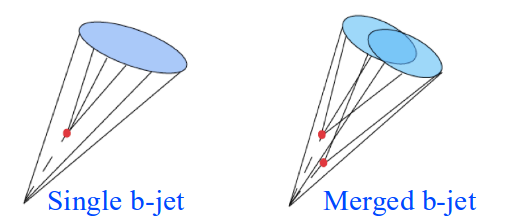
\includegraphics[width=0.8\textwidth]{FIGS/Single_b_Merged_bb.png}
% \caption{$b$-tagging algorithms select jets originating both from the fragmentation of single $b$-quark (``single'' $b$-jet, left image) or from the splitting of a gluon into a pair of close-by $b \bar{b}$ quarks (``merged'' $b$-jets, right image).}
% \caption{$b$-tagging algorithms select jets originating both from the fragmentation of single $b$-quark (``single'' $b$-jet, left image) or from the splitting of a gluon into a pair of close-by $b$-hadrons (``merged'' $b$-jets, right image).}
\caption{A $b$-jet can originate from the fragmentation of single $b$-quark (``single'' $b$-jet, left image) or from the fragmentation  of a pair of close-by $b$-quarks
%splitting of a gluon into a pair of close-by $b$-hadrons 
(``merged'' $b$-jets, right image).}
\label{fig:gbbcartoon}
\end{figure}



 

%------------------------------------------------------------------------
%\section{Physics Motivation}\label{sec:motivation}
%------------------------------------------------------------------------
%Reduced version
%In this section we briefly discuss two applications of the study and indentification of merged $b$-jets: the measurement of QCD $b$-quark production and the reduction of background in SM and Beyond the Standard Model (BSM) analyses.


Within the Standard Model (SM) a range of production channels exist for
heavy-quark jets, $\eg$ pure QCD production or in association with heavy bosons
($W, Z, H$). Furthermore, $b$-quarks enter in many collider searches, notably
because they are produced in the decays of various SM particles, \eg top
quarks and the Higgs boson (if light), and of numerous particles appearing
in proposed extensions of the SM. The ability to distinguish genuine $b$-quark jets from those produced via gluon splitting is thus of wide application. Here we briefly discuss three cases, the measurement of QCD $b$ quark production, the reduction of background in SM and BSM analyses with $b$ quarks in the final state, and studies of jet substructure.%
%
\\[5mm]
{\em The measurement of the inclusive $b$-jet spectrum}
\\[5mm]
The simplest and most fundamental measurement of heavy-quark jet production is
the inclusive heavy-quark jet spectrum, which is dominated by pure QCD
contributions.  Studies of QCD bottom jets production are of intrinsic interest
because of the correspondence between parton level production and the observed
hadron level, and their potential to provide information on the $b$-quark
parton distribution function, the only component of the proton structure
thought to be generated entirely perturbatively from the DGLAP evolution of the
other flavours.  The theoretical calculation of the inclusive
$b$-jet spectrum presents the striking feature of having rather important uncertainties ($\sim 50\%$), considerably larger than the
corresponding ones for the normal (light) jet inclusive spectrum ($\sim
10$-$20\%$), see for example~\cite{Frixione:1996nh}.  

The origin of these uncertainties are reviewed in a recent paper by Banfi, Salam and Zanderighi~\cite{Salam.AccurateHQ}, from which we have taken Fig.~\ref{fig:bjets_qcd}. Its top panel shows the $K$-factor, the ratio of the next-to-leading order (NLO) to the leading order (LO) cross section, obtained with MCFM for the LHC design energy  ($pp$, $\sqrt{s}= 14$ TeV).
\begin{figure}[tp]
\centering
%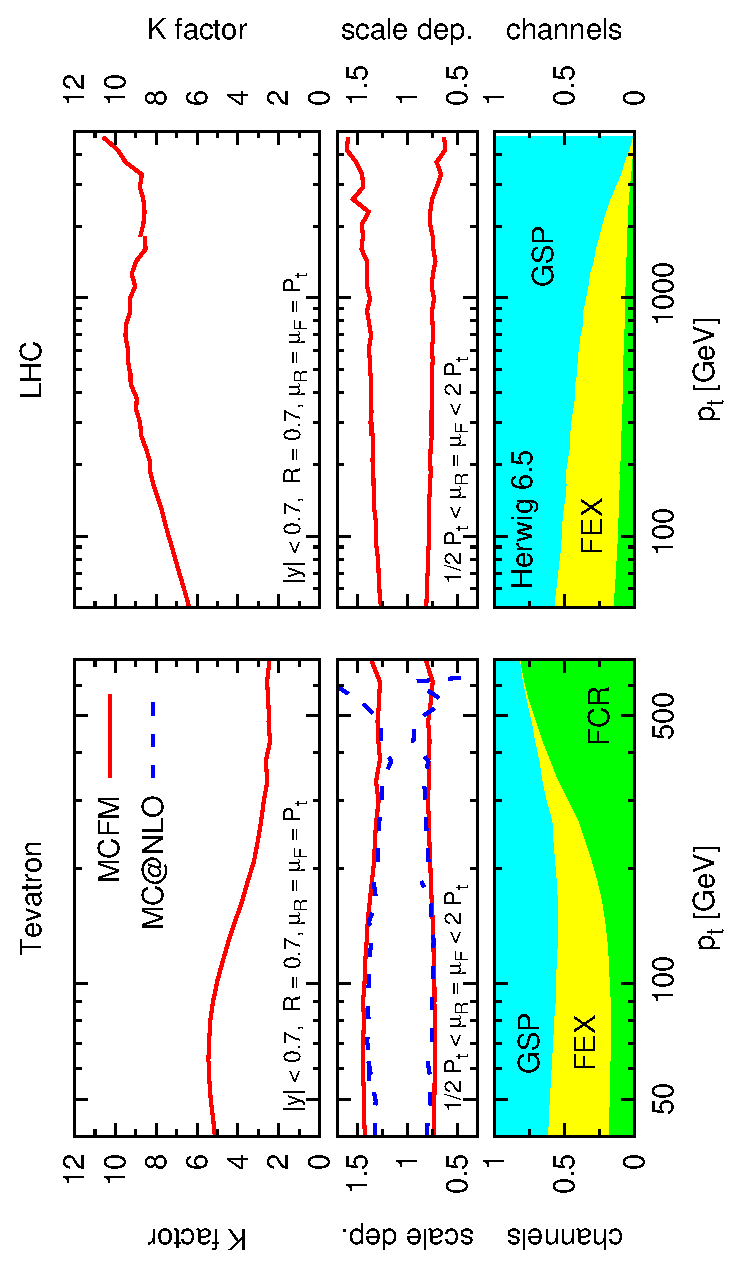
\includegraphics[height=0.7\textwidth,viewport=20 305 340 590,clip,angle=270]{FIGS/bjets_qcd.eps}
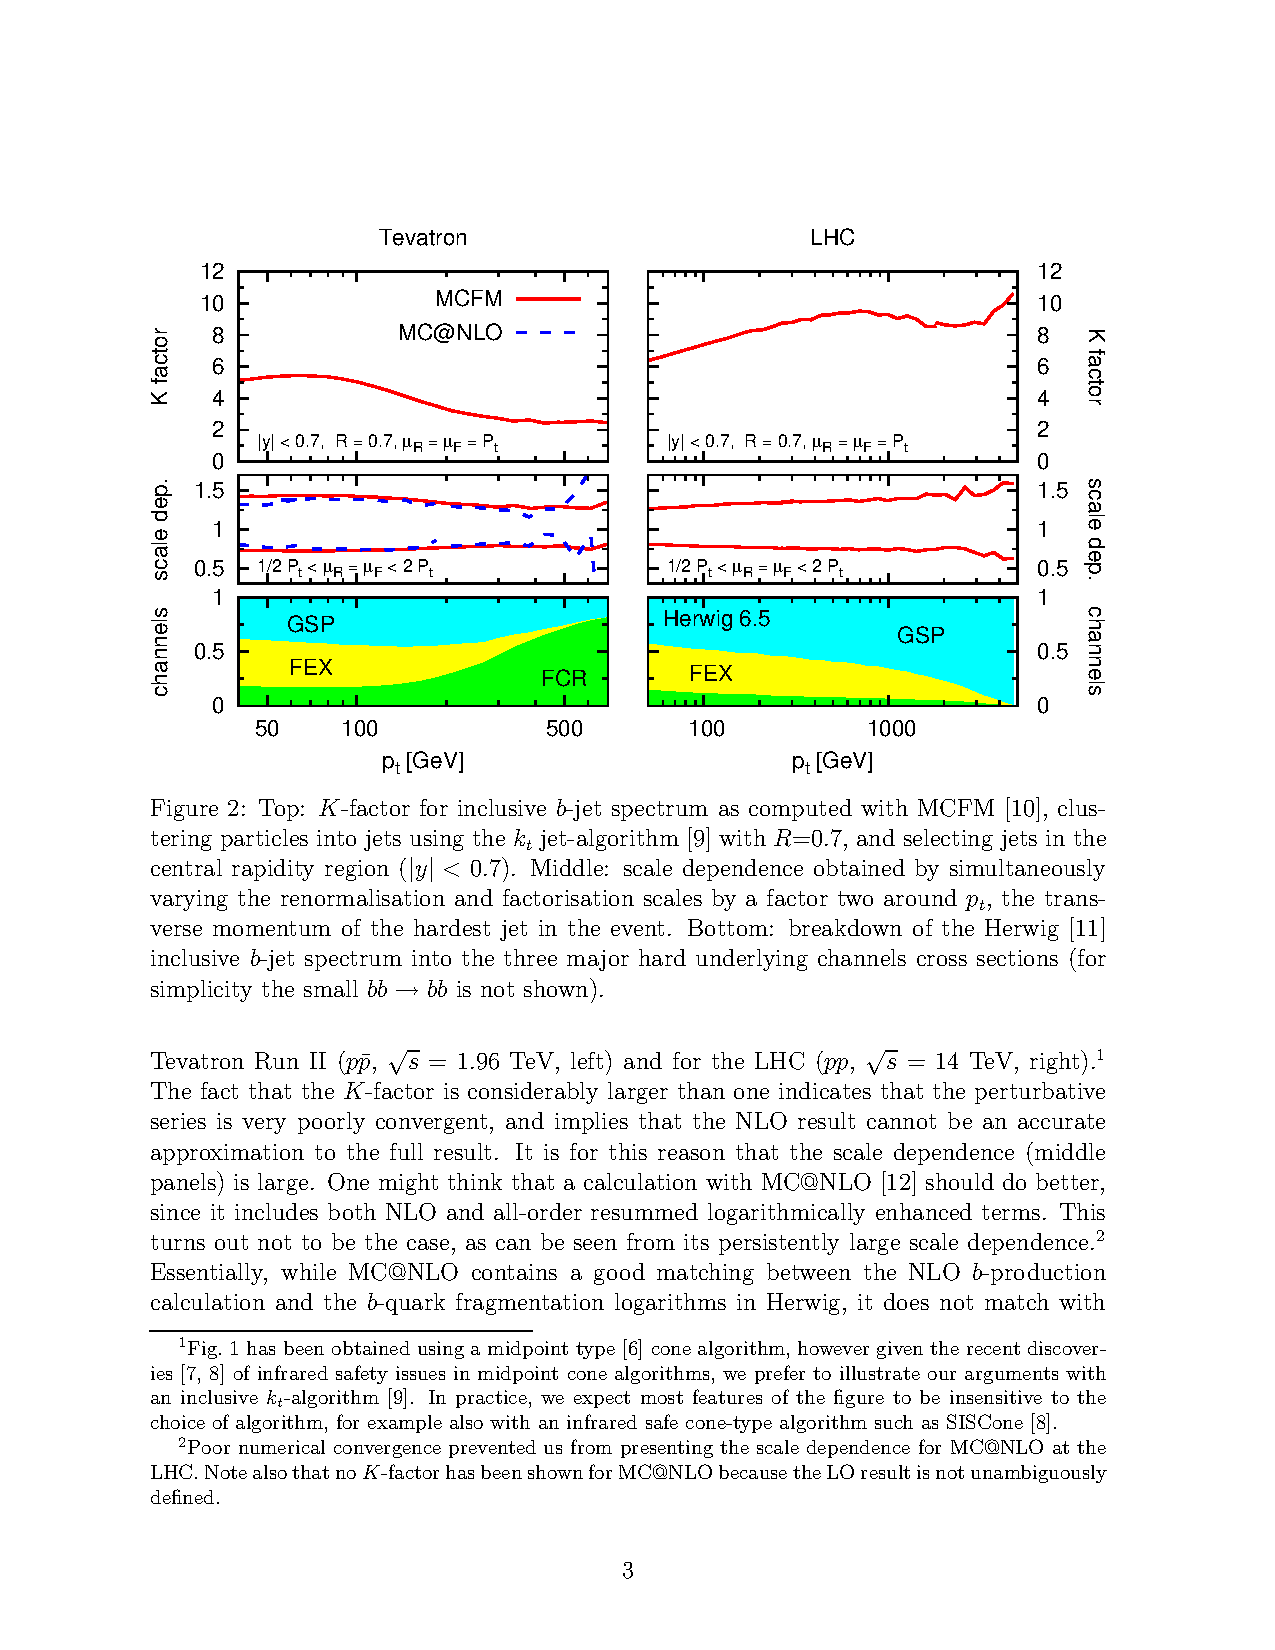
\includegraphics[height=0.7\textwidth,viewport=300 410 530 690,clip]{FIGS/bjets_qcd.pdf}
  \caption{Top: $K$-factor for inclusive $b$-jet spectrum taken
  from~\cite{Salam.AccurateHQ}, clustering particles into jets using the $k_t$
  jet-algorithm~\cite{kt1}  with $R$=0.7, and selecting jets in the central
  rapidity region ($|y| <0.7$). Middle: scale dependence obtained by
  simultaneously varying the renormalisation and factorisation scales by a factor
  two around $\pt$, the transverse momentum of the hardest jet in the event.
  Bottom: breakdown of the Herwig \cite{Herwig} inclusive $b$-jet spectrum into
  the three major underlying channels, flavor creation (FCR) flavor excitation
  (FEX) and gluon splitting (GSP).}
  \label{fig:bjets_qcd}
\end{figure}
The fact that NLO terms are considerably larger than the LO ones indicates
that the perturbative series is very poorly convergent, and implies that the
NLO result cannot be an accurate approximation to the full result.
It is for this reason that the scale dependence (middle panels) is large.  The
poor convergence of the perturbative series is related to the different
channels for heavy quark production. At leading order only the so-called
flavour creation channel (FCR) is present, $\ell \ell \to b\bb$, where $\ell$
is a generic light parton (quark or gluon), see fig.~\ref{fig:qcd_diagrams}.
%
\begin{figure}[h!]
\centering
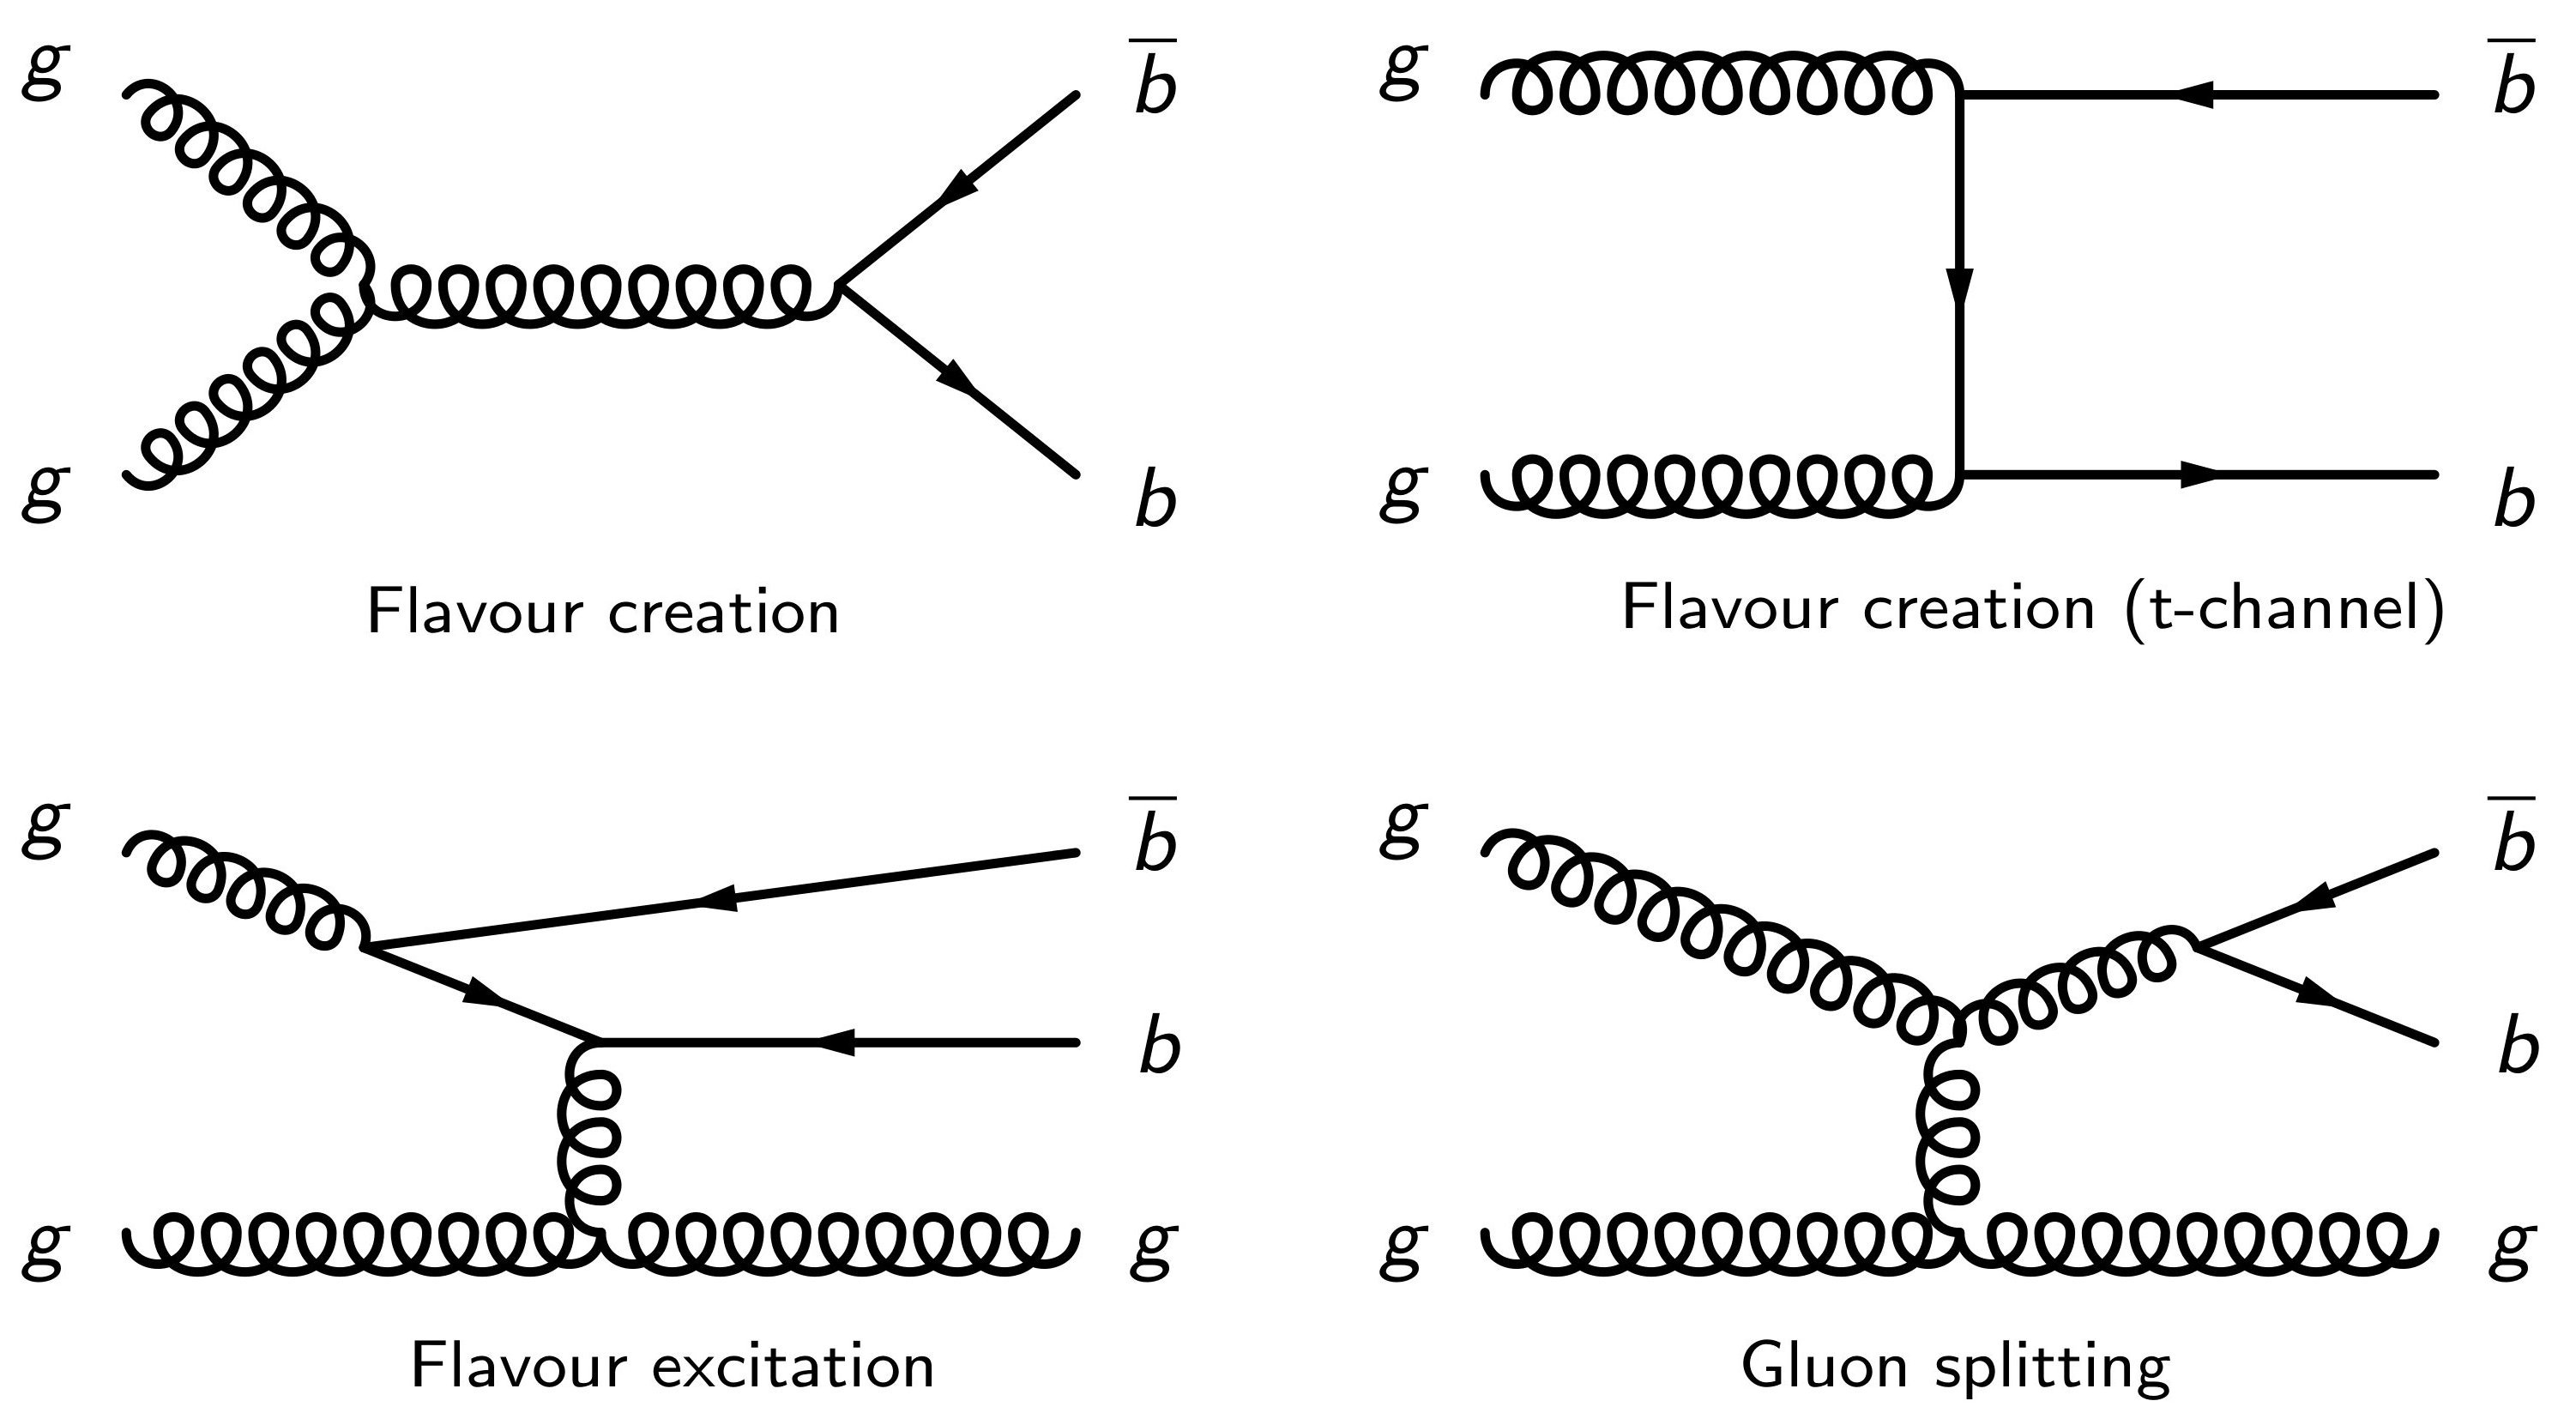
\includegraphics[width=0.32\textwidth,viewport=0 880 1500 1600,clip]{FIGS/bb_diagrams.jpg}
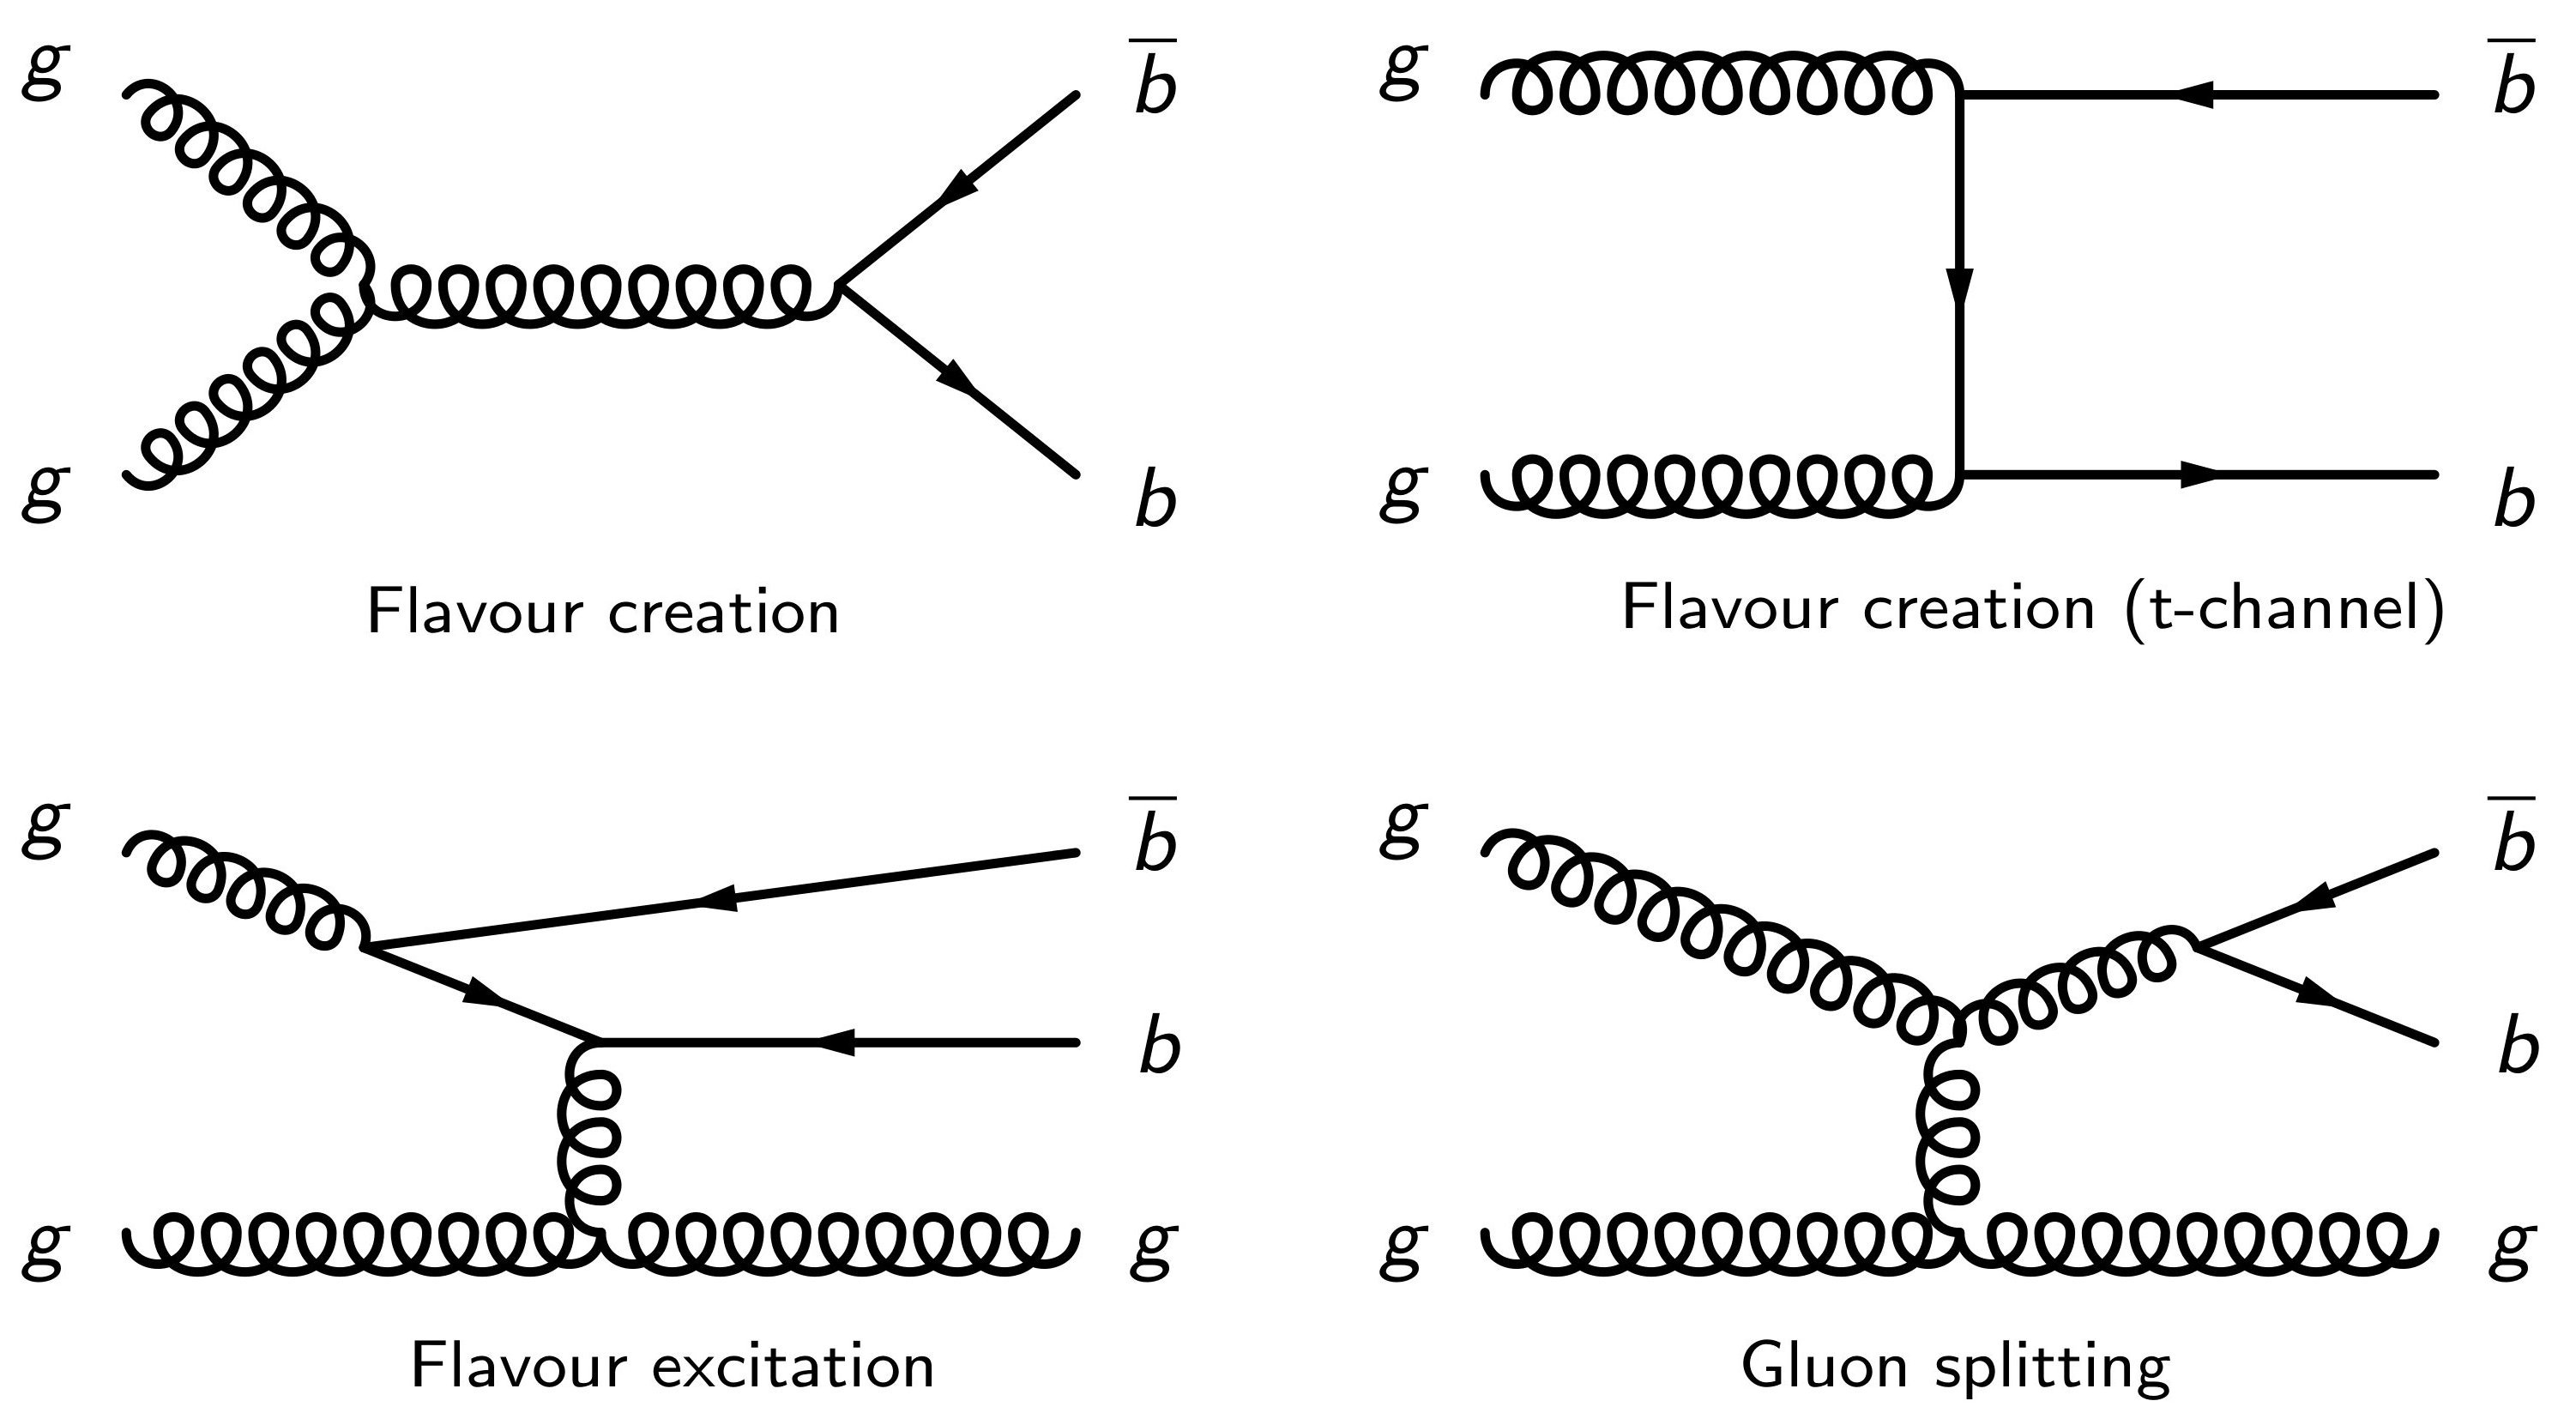
\includegraphics[width=0.32\textwidth,viewport=1600 0 3100 820,clip]{FIGS/bb_diagrams.jpg}
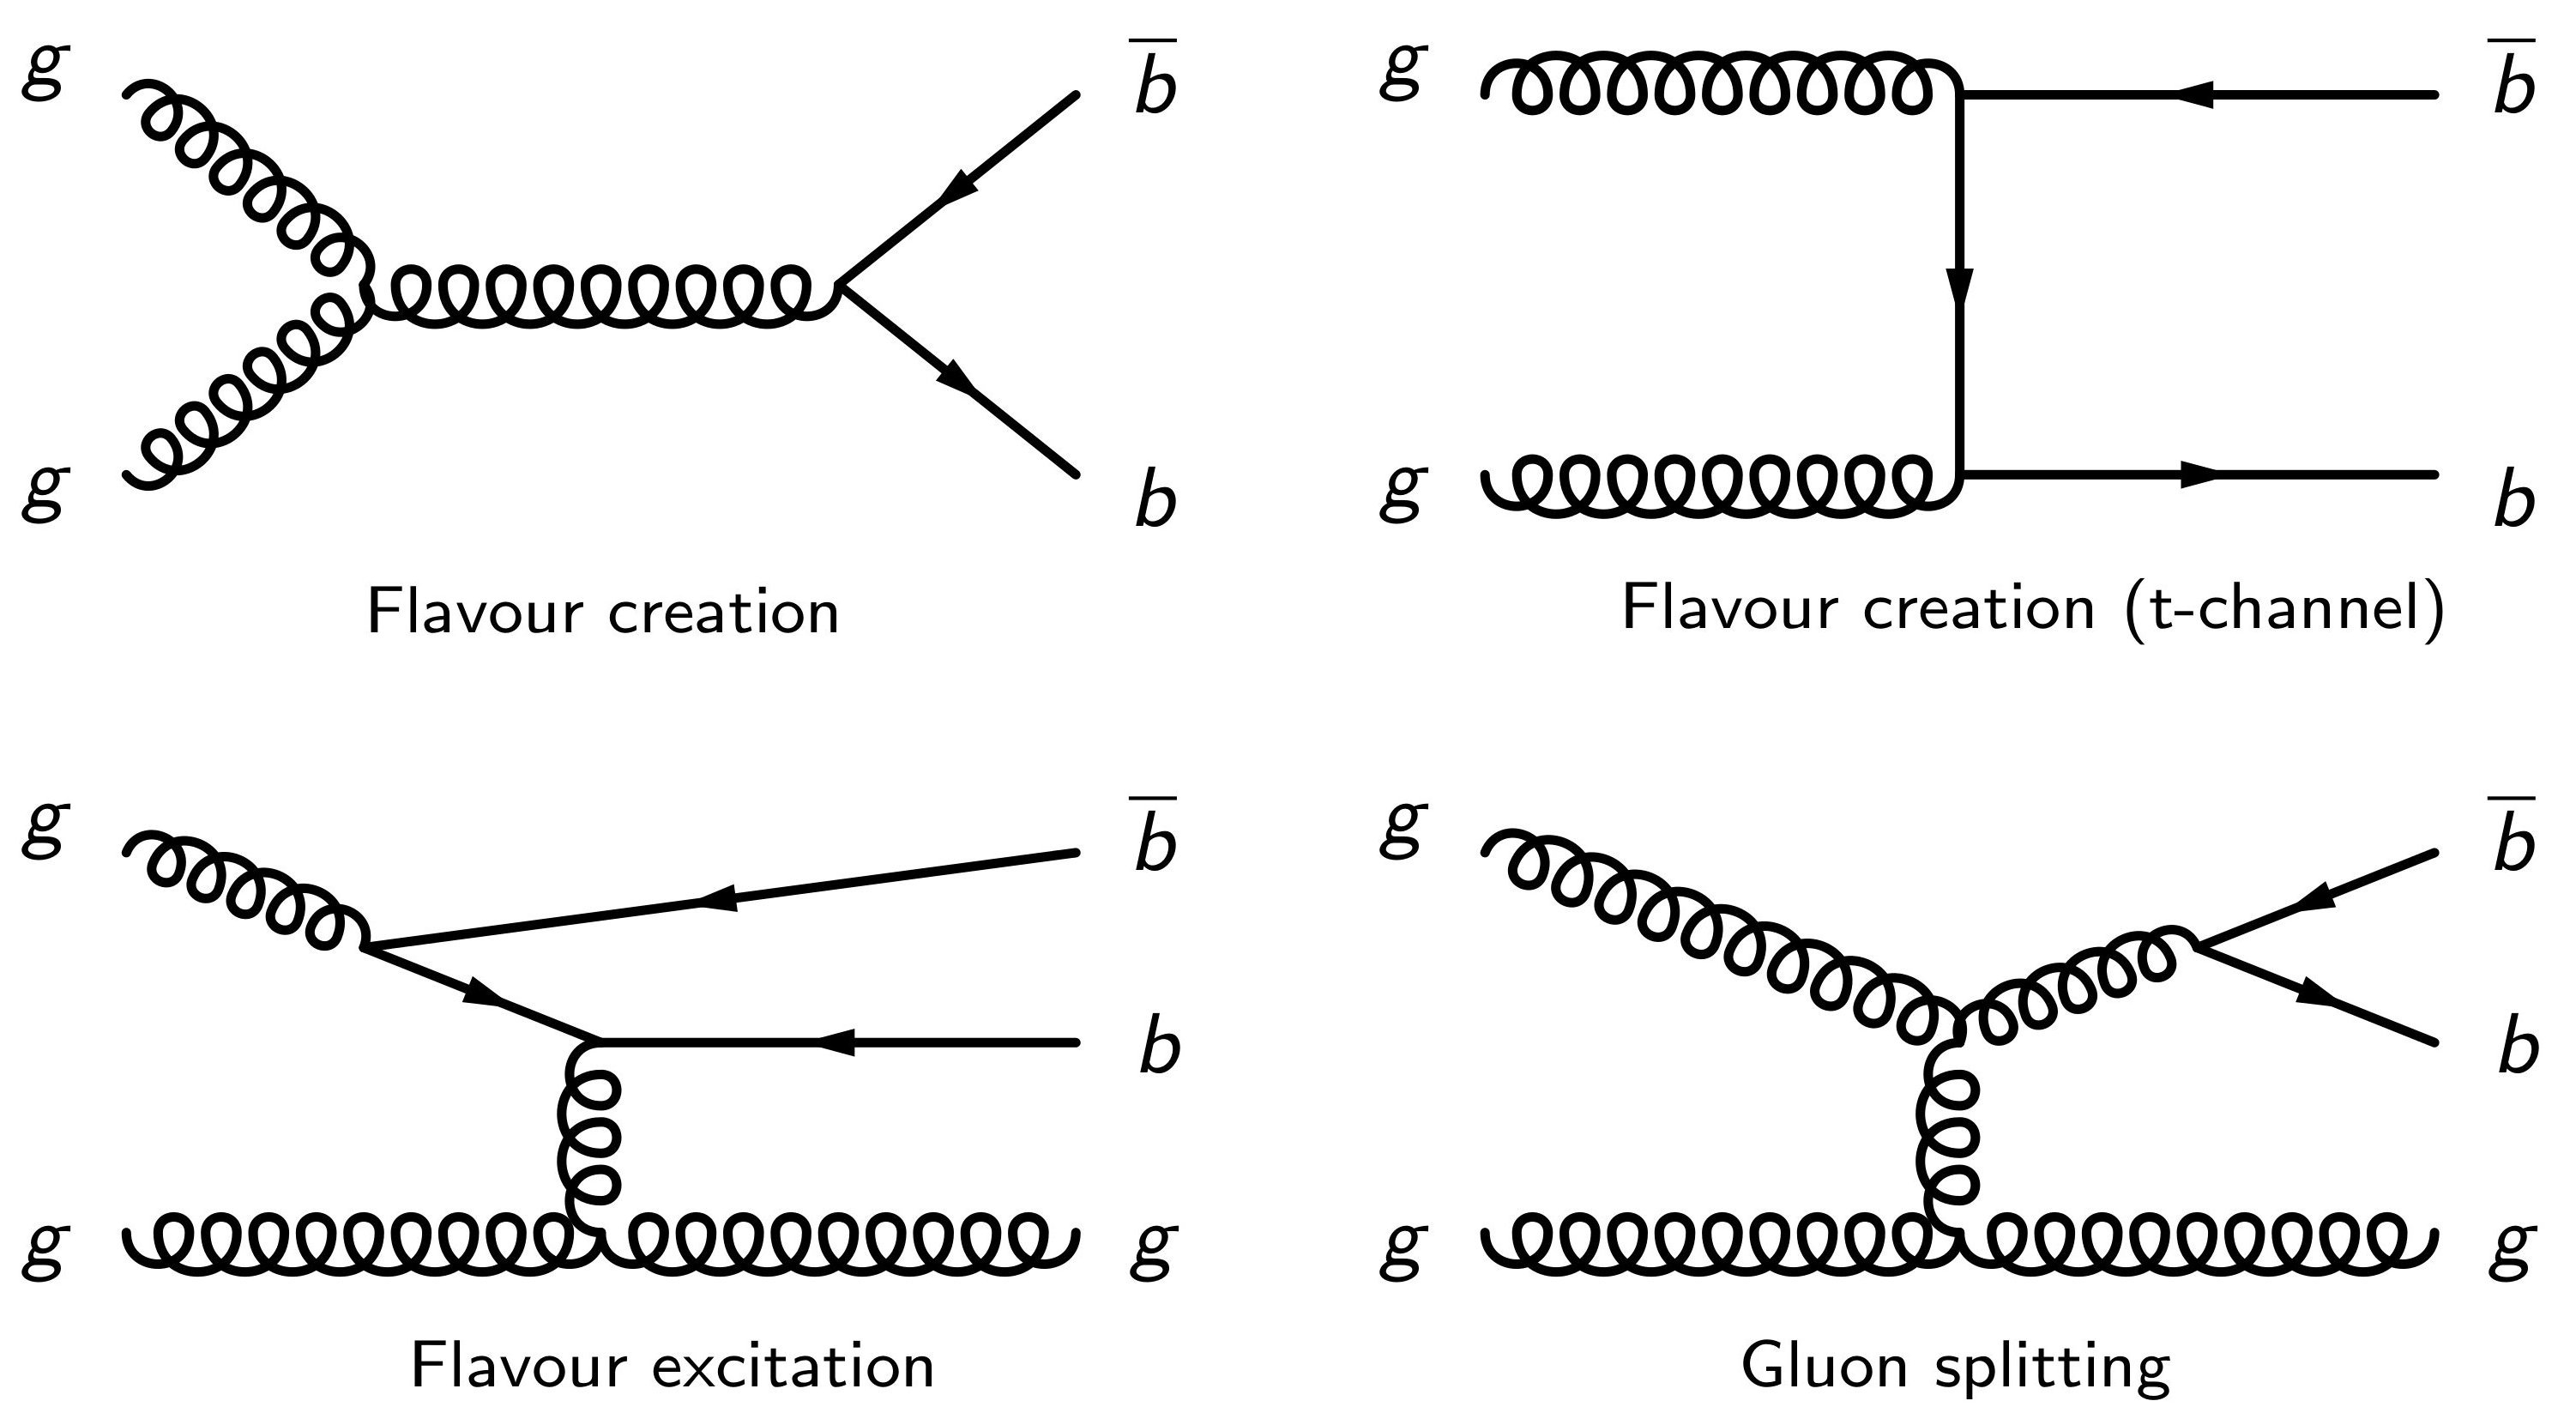
\includegraphics[width=0.32\textwidth,viewport=0 0 1500 820,clip]{FIGS/bb_diagrams.jpg}
\caption{Representative diagrams of the three channels contributing to QCD $b$-quark production up to NLO. The flavour creation channel (left) is the only one present at LO. At NLO, two new channels open up, referred to as gluon splitting (center) and  flavour excitation (right).}
\label{fig:qcd_diagrams}
\end{figure}
%
At NLO, two new channels open up, often referred to as flavour excitation (FEX) and gluon splitting (GSP). In the former, a gluon from one of the incoming hadrons splits collinearly into a $b \bar{b}$-pair and one of those $b$-quarks enters the hard $b\ell \to b\ell$ scattering. In the gluon splitting process, the hard scattering LO diagram is of the form $\ell \ell \to \ell \ell$, and one of the final-state light partons (at NLO always a gluon) splits collinearly into a $b \bar{b}$-pair that the clustering algorithm can classify within the same jet. A jet containing both $b$ and $ \bar{b}$ is considered to be just a $b$-jet in standard definitions.
The various channels can be conveniently separated with a parton shower Monte Carlo generator such as Herwig~\cite{Herwig}, where one can determine the underlying hard channel from the hard process in the event record. Their relative contributions to the total $b$-jet spectrum are shown in the bottom panel of fig.~\ref{fig:bjets_qcd}.  One sees that the supposedly LO channel (FCR) is nearly always smaller than the two channels that enter only at NLO (FEX and GSP). %\footnote{This is because both NLO channels receive a strong enhancement from collinear logarithms, going as $\as^2 (\as \ln(\pt/\Mb))^n$ for flavour excitation~\cite{DGLAP} and $\as^2 \cdot \as^n \ln^{2n-1}(\pt/\Mb)$ for gluon splitting ($n\ge 1$)~\cite{bmult}}.

The largest residual uncertainties are associated with the channel with the
most logarithms, gluon splitting. This channel however does not even correspond
to one's physical idea of a $b$-jet, \ie the one induced by a hard $b$-quark, and it
seems somehow unnatural to include it at all as part of one's $b$-jet spectrum.
Reference~\cite{Salam.AccurateHQ} thus proposes a new approach to improving the accuracy of the prediction of
the $b$-jet spectrum, where $b$-jets definition maintains the correspondence
between partonic flavour and jet flavour. Specifically, a jet containing equal
number of $b$-quarks and $b$-antiquarks is considered to be a light jet, so
that jets identified as gluon splitting are removed from the $b$-jet spectrum. %
%
\\[5mm]
{\em Rejection of background in SM analyses and beyond-SM searches}
\\[5mm]
Efficient tagging of merged $b$-jets from gluon splitting can provide an important handle to understand, estimate and/or reject $b$-tag backgrounds to Standard Model and new physics searches at the LHC.

Standard Model physics analyses that rely on the presence of $b$ quarks in the final state such as top quark physics, either in the $t\bar{t}$ or the single top channels, and associated
Higgs production: $WH\rightarrow\ell\nu b\bar{b}$ and $ZH\rightarrow\nu\nu
b\bar{b}$, suffer from reducible backgrounds from QCD (that can produce $b$-jets from gluon splitting) and, most importantly, from the irreducible background due to  
$W$ bosons produced in association with $b$ quarks.  Fig.~\ref{fig:Wplusb} shows
the two leading order processes that give rise to $W$ bosons with at least one
$b$-jet. In the first process, which can be thought of as a higher order correction to $W$ + jets production, the $b$ quark pair is produced at small angles by gluon
splitting and can often be reconstructed as a merged jet.
\begin{figure}[hp]
\centering
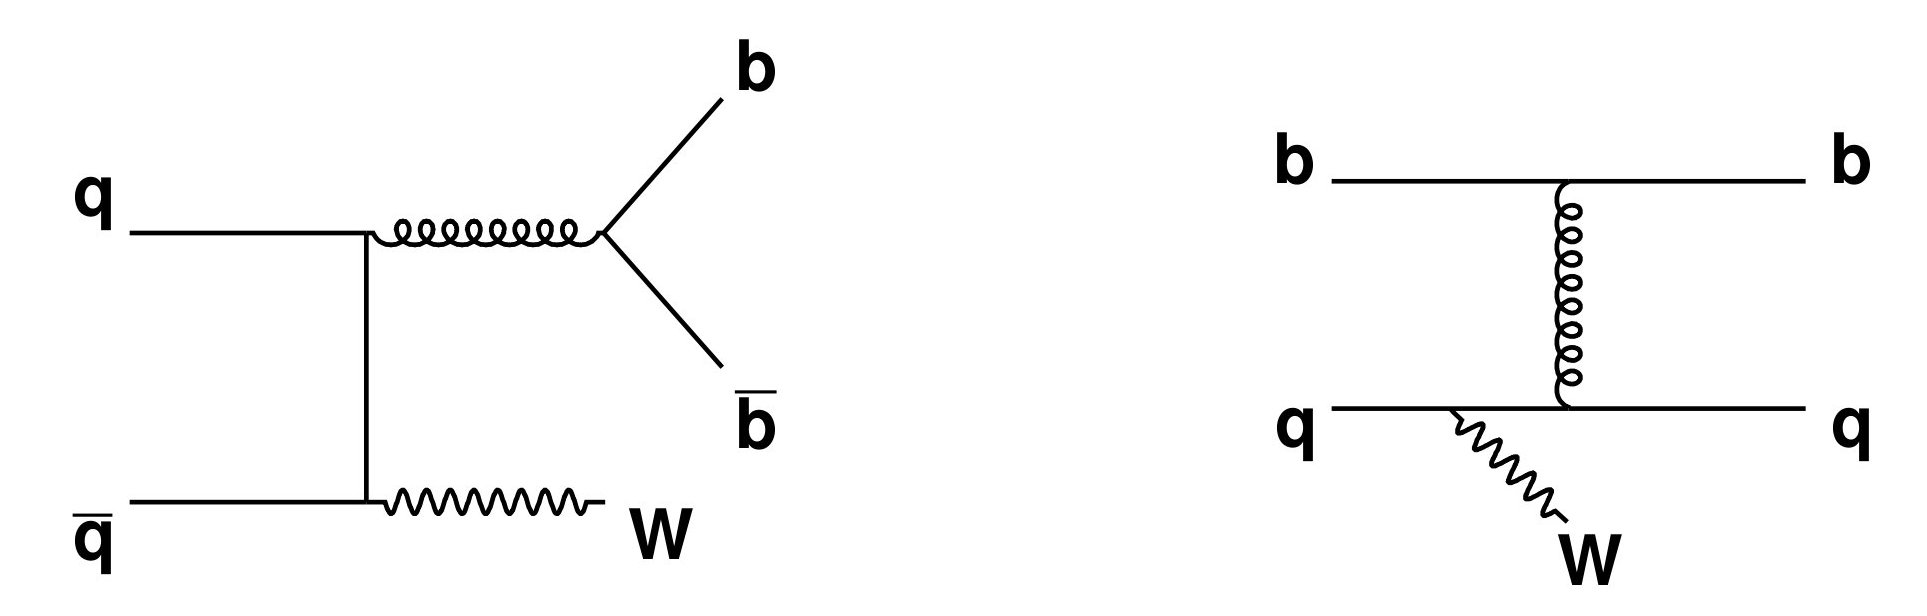
\includegraphics[width=0.6\textwidth]{FIGS/Wbb_diagram.jpg}
\caption{Leading order Feynman diagrams for $W$ production in association with $b$ quarks.}
\label{fig:Wplusb}
\end{figure}
NLO calculations of the production of $W$ bosons and two jets with at least one $b$ quark at the LHC for jet $\pt > 25$ GeV, and $|\eta| < 2.5$~\cite{Campbell:2006} indicate that the cross section for $W(b\bar{b})j$ is almost a factor of two higher than $Wb\bar{b}$, and about a third of $Wbj$, where  $W(b\bar{b})j$ denotes the case in which the two $b$ quarks are merged into the same jet. 

New physics searches with $b$ quarks in the final state can also greatly benefit from rejection of QCD and $W+b$ backgrounds with $b$-jets arising from gluon splitting. For example consider the search for supersymmetry in the \met\ + $b$-jets channel~\cite{ATLAS-CONF-2011-098}. Within the framework of a generic $R$-parity conserving minimal supersymmetric extension of the SM The coloured superpartners of quarks and gluons, the squarks and gluinos, are expected to be copiously produced via the strong interaction at the LHC. The
partners of the right-handed and left-handed quarks, qR and qL, can mix to form two mass eigenstates, and these mixing effects being proportional to the corresponding fermion masses, they are expected to become most important for the third generation to yield sbottom ($b_1$ ) and stop ($t_1$ ) mass eigenstates significantly lighter than other squarks. Both sbottom and stop chain decay to $b$ quarks and the lightest supersymmetric particle, producing the expected signal of \met\ + $b$-jets. 
%
%
\\[5mm]
{\em Jet substructure and boosted objects}
\\[5mm]
At the LHC, many of the particles considered to be heavy at previous accelerators will be frequently produced with a transverse momentum greatly exceeding their rest mass. Good examples are the electro-weak gauge bosons $W^\pm$ and $Z^0$, the top quark, the Higgs boson or bosons and possibly other new particles in the same mass range. These boosted objects, produced either because they recoil against other energetic objects or because they arise from decays of even heavier BSM particles, can form upon decay a highly collimated topology too close to be resolved by a jet algorithm. For theses cases, sophisticated tools have been developed in the last years~\cite{boost2010,boost2010b} to analyse the substructure of the ensuing jet and reveal its heavy-particle origin. 

The study of $b\bar{b}$ jets from gluon splitting is an ideal testbed for studying jet substructure in data, as it provides a large supply of boosted, merged jets. Furthermore, understanding $g\rightarrow b \bar{b}$ jets is important as they are themselves the background to boosted object searches, like $Z\rightarrow b\bar{b}$ or $H\rightarrow b \bar{b}$.  In particular, it has recently been suggested~\cite{Butterworth:2008iy} that $WH$ and $ZH$ production become potential discovery and analysis channels by restricting one’s attention to the $\sim5$\% of events in which the vector and Higgs bosons have large transverse momentum, ${\pt}_H\gtrsim200$ GeV. Understanding the much more common QCD events with merged $b\bar{b}$ jets will be essential before attempting to measure these rare final states.



%%%%%%%%%%%%%%%%%%%%%%%%%%%%%%%%%%%%%%%%%%%%%%%%%%%%%%%%%%%%%%%%%%%
%     (above) End of motivation 
%     (below) Our work, plus content
%%%%%%%%%%%%%%%%%%%%%%%%%%%%%%%%%%%%%%%%%%%%%%%%%%%%%%%%%%%%%%%%%%%




There are two possible strategies to attempt to identify $b$-jets containing two $b$-hadrons. One of them relies on the direct reconstruction of the two $b$-decay secondary vertices~\cite{CDFAzimutalCorrelation}. This %has the further advantage of allowing 
allows the measurement of the angular separation between the $b$-hadrons, but suffers from the low efficiency of a double $b$-tag requirement plus additional reconstruction inefficiencies at small angular separation between the two $b$-hadrons. In this thesis we develop an alternative method that does not rely on explicit vertex finding, but exploits the substructure differences between single and merged $b$-jets, combining them in a multivariate analysis. 

Chapter~\ref{chap:theory} describes the theoretical framework, with emphasis in the theory of the strong interactions and the aspects that are important for the understanding of the hadronic final state in hadronic collisions. The LHC and the ATLAS detector components  are described in Chapter~\ref{chap:lhc_atlas}, together with a summarization of the detector conditions during 2011 data taking.  Chapter~\ref{chap:reco} details how jet reconstruction and calibration are performed at ATLAS and describes the procedure for the identification of $b$-quark jets. Chapter~\ref{chap:kinematic} presents the analysis of jet shape and substructure variables for the discrimination between single and double $b$-hadron jets. The validation of the variables in 2011 data is also included.   The construction of the multivariate discriminator  and the discussion of the systematic uncertainties are presented in Chapter~\ref{chap:mva}. 

{\sc To do}
Preliminary results for the measurement of the fraction of double $b$-hadron jets in data are discussed in Chapter~\ref{chap:gbbfraction}. 

Finally, chapter~\ref{chap:conclusions} summarizes the results. 
 
%\%
%
%%%%%%%%%%%%%%%%%%%%%%%%%%%%%%%%%%%%%%%%%%%%%%%%%%%%%%%%%%%%%%%%%%%%%%%%%%%%%%%
% Theory
%%%%%%%%%%%%%%%%%%%%%%%%%%%%%%%%%%%%%%%%%%%%%%%%%%%%%%%%%%%%%%%%%%%%%%%%%%%%%%%
%
%\chapter{Quantum Chromodynamics}
\chapter{The theory of the strong interactions}

%------------------------------------------------------------------------
\section{The Standar Model}\label{sec:qcdintro}
%------------------------------------------------------------------------

%From Kirsten
The Standar Model (SM) describes particles interaction. It is a coherent theory that describes the behavior of all experimentally-observed particles under the influence of the electromagnetic force, the weak force, and the strong force.
The most conspicuous omission is a description of gravity, which is fortunately negligible at the distance and energy  scales usually considered in particle physics experiments.
The three theoretical building blocks of the SM, QED, EW and QCD are all derived from imposing Lorentz invariant symmetries onto interacting fields.
QED~\cite{PhysRev.75.486} describes the interaction of charged particles via the exchange of charge-neutral photons. It is formulated by imposing a U(1), or rotational, symmetry onto the simplest field Lagrangian that obeys the correct equations of motion. %->gauge fields, spin 1 bosons, the photons.
The description of the weak force builds from the QED Lagrangian. This time, an SU(2) symmetry, which corresponds to rotations of 2-dimensional vectors, combines with the U(1) symmetry from QED to produce additional gauge fields. The gauge fields mix with the gauge field from QED to form $W^+$, $W^-$ and $Z^0$ bosons that transmite the weak force. %.. masses of the gauge bosons, theory and experiments
At masses higher than the $Z$ mass, the elctromagnetic and weak forces unify into a single force, known as the electroweak force~\cite{Glashow1961579}~\cite{Salam1964168}~\cite{PhysRevLett.19.1264}.
%See confirmation of the Electroweak theory 
%Z and W discovery ~\cite{Banner1983476}~\cite{Arnison1983398}


%------------------------------------------------------------------------
%\subsection{Quantum Chromodynamics}\label{sec:qcd}
%------------------------------------------------------------------------


%------------------------------------------------------------------------
\section{Jet physics}\label{sec:jets}
%------------------------------------------------------------------------


Due to confinement quarks do not exist in isolation, but rather transform into stable color-singlet hadrons. Consequently, the experimental signature of quarks and gluons are the final state hadrons. The packet of particles produced tends to travel collinearly with the direction of the initiator quark or gluon. The result is a ``spray'' of hadrons (also photons and leptons) entering the detector in place of the original parton; these clusters of objects are what we define as jets.
%using inclusive hadronic event shapes to demonstrate the presence of jets.

The evolution from a single parton to an ensemble of hadrons accurs through the processes of parton showering and hadronization. Since the strong coupling constant grows with increasing distance between color charges, a strong color potential forms as the parton from the ``hard'' (high $Q^2$) scattering process separates from the original hadron. This large potential causes quark$/$antiquark pairs ($q\bar{q}$) to be created, each carrying some of the energy and momentum of the original partons. As these new partons move away from one another, yet more color potentials are formed, and the process repeats. Thus from one parton a shower of partons appears, traveling along the same direction as the original.  This process continues until there is no longer enough energy to create additional $q\bar{q}$ pairs, and instead the remaining partons combine to form stable hadrons. Since this progression involves successively lower energies and lower momentum transfers, perturbative QCD cannot describe the full process.  The hadronization process then cannot be calculated from first principles, but has to be modelled (see next section). 
%In real life (data), fluctuations arise from the quantum mechanics of the underlying theory.  In generators, Monte Carlo (MC) techniques are used to select all relevant variables according to the desired probability distributions, and consecuently ensure (quasi-)randomness in the final state. This is the subject of the next section.
%From Pythia's manual http://arxiv.org/abs/hep-ph/0603175

The first evidence for jet production was observed in $e^+e^-$ collisions at the SPEAR storage ring at SLAC in 1975~\cite{PhysRevLett.35.1609}. 
%In order to determine how jetlike an event was, they calculated the sphericity, a quantity between 0 and 1, with values approaching to 1 meaning an isotropic phase-space with high multiplicity; and  0, for events with bounded transverse momenta. The data agreed with the jet model predicted by the Monte Carlo simulation.

\subsection{Monte Carlo tools}

%In high-energy processes such a those at the LHC, the low value of the strong force coupling constant can be exploited, allowing perturbative techniques to be used to calculate physical processes.  We can use the perturbative language to describe the shoft-distance interactions of quarks, leptons and gauge bosons. For leptons and gauge bosons, that lack of colour charge, this language is adequate. However for the interaction of quark and gluons in hadron collisions, this picture must be completed with the structure of incoming hadrons and a model for the fragmentation and decay (hadronization) process, that cannot be calculated from first principles.

%From Gavins's http://arxiv.org/abs/1011.5131
Knowing QCD predictinos is crucial in the design of methods to search for new physics, as well as for extracting meaning from data. Different techniques can be used to make QCD predictions at hadron colliders, and in particular at the LHC. The so called Matrix Element Monte Carlos use direct perturbative calculations of the cross-section matrix elements in powers of the strong coupling constant, $\alpha_s$, for each relevant partonic subprocesses. Leading order (LO) and next-to-leading order (NLO) calculations are available for many processes.   These ``fixed-order predictions'' include the first terms in the QCD perturbative expansion for a given cross-section; as more terms are involved in the expanstion, an improvement in the accuracy of the prediction is expected.  The complexity of the calculations increased significantly with the number of outgoing legs, limiting available results to those with at most three outgoing partons. Matrix element MC programs include {\sc Alpgen}~\cite{ALPGEN}, {\sc Madgraph}~\cite{MADGRAPH} and others.
%Are these characteristics representative of the ‘typical’ situation for collider observables? We only have predictions up to NNLO in a handful of cases (see below) and in those it is. In cases where wejust have NLO predictions, the features of large ‘K-factors’ (NLO/LO enhancements) with a reduced NLO uncertainty band are not uncommon, suggesting that beyond NLO corrections should be small. Exceptions are known to arise in two types of case: those where new enhanced partonic scattering channels open up at NLO (or beyond); and that involve two disparate physical scales.
%Technically, one main consideration has so far limited the range of processes for which NLO results exist: the availability of the loop amplitude. Until recently loop amplitudes were usually calculated semi-manually for each process. The complexity of the calculations increased significantly with the number of outgoing legs, limiting available results to those with at most three outgoing partons. Many NLO results for 2 → 2 and 2 → 3 processes are incorporated into programs such as NLOJ ET++ for jet production [65], MCFM for processes with heavy quarks and/or heavy electroweak bosons [66]


An alternative approach is applied by the so called Monte Carlo parton shower programs. These simulation programs use LO perturbative calculations of matrix elements for $2 \rightarrow 2$ processes, relying on the parton shower to produce the equivalent of multi-parton final state.  {\sc Pythia}~\cite{PYTHIA6} and {\sc Herwig}$++$~\cite{HerwigPP} are the most commonly used parton shower Monte Carlos together with {\sc SHERPA}. % and others.  
%how to get a parton shower event
%A quantity called Sudakov form factor (P (no emission above kt ) ≡ ∆(kt , Q)) allows us to easily calculate the distribution in transverse momentum of the gluon with largest transverse momentum in an event.
%FORMULA
%This distribution is easy to generate by Monte Carlo methods: take a random number r from a distribution that is uniform in the range 0 < r < 1 and find the kt1 that solves ∆(kt1 , Q) = r. Given kt1 we also need to generate the energy for the gluon, but that’s trivial. If we started from a q q system (with some randomly generated orientation), then this gives us a q q g system. As a next step one can work out the Sudakov form factor in the soft/collinear limit for there to be no emission from the q q g system as a whole above some scale kt2 (< kt1 ) and use this to generate a second gluon. The procedure is then repeated over and over again until you find that the next gluon you would generate is below some non-perturbative cutoff scale Q0 , at which point you stop. This gives you one ‘parton shower’ event.
%The above shower descriptions hold for final-state branching. With initial-state hadrons, one also needs to be careful with the treatment of the PDFs, since the collinear splitting that is accounted for in the parton shower is also connected with the way the PDF is built up at the scale of the hard scattering.


The Monte Carlo generators must account for and correctly model the showering of partons. To approximate the energy-evolution of the shower, the DGLP (REFEERNCIAS?) equations that describe the evolution of the PDFs with changing energy scale can be used. The separation of radiation into initial- (before the hard scattering process takes place) and final-state showers is arbitrary, but sometimes convenient.  In both initial- and final-state showers, the structure is given in terms of branchings $a \rightarrow bc$: $q \rightarrow qg$, $q \rightarrow q\gamma$, $g \rightarrow gg$ and $g \rightarrow q\bar{q}$. Parton $b$ carries a fraction $z$ of the energy of the mother energy and parton $c$ carries the remaining $1-z$ (the term ``partons'' is including the radiated photons).  In turn, daughters $b$ and $c$ may also branch, and so on. Each parton is characterized by some evolution scale, which gives an approximate sense of time ordering to the cascade. In the initial-state shower,  the evolution scale values are gradually increasing as the hard scattering is approached, while  these values decrease in the final-state showers. The evolution variable of the cascade in the case of {\sc Pythia} generator, $Q^2$, has traditionally been associated with the $m^2$ of the branching partons\footnote{The final-state partons have $m^2>0$. For initial-state showers the evolution variable is $Q^2=-m^2$, which is required to be strictly increasing along the shower.}. In the recent version of {\sc Pythia} a $p_{\perp}$-ordered shower algorithm, with $Q^2=p_{\perp}^2$ is available, and the shower evolution is cut off at some lower scale  $Q_0$ typically arond 1 GeV for QCD branchings. {\sc Herwig}$++$ provides a shower model which is angular-ordered.

There are two leading models for the description of the non-perturbative process of hadronization, after parton showering. {\sc Pythia} uses the Lund string model of hadronization to form particles~\cite{LUNDMODEL}.  This model involves stretching a colour ``string'' across quarks and gluons and breaking it up into hadrons.% In this model, the color force felt between partons is described as a string connecting them. When the potential is large enough, the string snaps into two, each broken end links a new parton to the one of the original partons.
{\sc Herwig}$++$ utilizes the cluster model of hadronization. In this model each gluon is split into a $q\bar{q}$ pair and then quarks and anti-quarks are grouped into colourless ``clusters'', which then give the hadrons.

Hadronization models involve a number of ‘non-perturbative’ parameters. The parton-shower itself involves the non-perturbative cut-off $Q^2_0$ . These different parameters are usually tuned to data from the LEP experiments.


In addition to the hard interaction that is generated by the Monte Carlo
simulation, it is also necessary to account for the interactions between the incoming proton  remnants. This is usually modelled through multiple extra $2\rightarrow 2$ scattering, occurring at a scale of a few GeV. This effect is known as multiple parton interactions (MPIs). In addition, these partons may radiate some of their energy, either before or after the hard interaction.  All the parton interactions, which are note calculated form the hard scattering process, are grouped together in the term underlying event. The modelling of the underlying event is crucial in order to give an accurate reproduction of the (quite noisy) energy flow that accompanies hard scatterings in hadron-collider events.

It should be stressed that these multiple parton interactions are a separate effect from the multiple proton interactions that may occur in each collision event in the LHC. These multiple proton collisions are referred to as pileup, and are not included in the definition of the underlying event. 

No precise model exists to reproduce the unerlying event activity. This activity is instead also adjusted to reproduce available experimental data. A specific set of chosen parameters for a generator is referred to as a ``tune''.  

The two Monte Carlo generators used in this analysis are summarized below, indicating the particular versions and tunes that were implemented.


\subsubsection{Pythia}

{\sc Pythia} event generator has been used extensively for $e^+ e^-$, $ep$, $pp/p\bar{p}$ at LEP, HERA, and Tevatron, and during the last 20 years has probably been the most used generators for LHC physics studies.  {\sc Pythia} contains an extensive list of hardcoded subprocesses, over 200, that can be switched on individually. These are mainly 2$\rightarrow$1 and  2$\rightarrow$2, some  2$\rightarrow$3, but no multiplicities higher than that. Consecutive resonance decays may of course lead to more final-state particles, as will parton showers.

As mentioned above, in this MC generator, showers are ordered in transverse momentum~\cite{Pythia_partonshowers} both for ISR and for FSR. Also MPIs are ordered in $\pt$~\cite{Pythia_mpi}. Hadronization is based solely on the Lund string fragmentation framework.
%the Field–Feynman model http://www.sciencedirect.com/science/article/pii/0550321378900159 (sent pdf by email, only accesible from cern)
% a few years later kickstarted the whole field of hadronization studies by Monte Carlo simulation
%On the Lund's String model
%Now consider a simple qqbar two-parton event further. As thea q and qbar move apart from the creation vertex, say along the ±z axis, the potential energy stored in the string increases, and the string may break by the production of a new qprima qbarprima pair, so that the system splits into two colour-singlet systems qqbarprima and qprima qbar. These two systems move apart, and a widening no-field region opens up in between, Fig. 13b. For simplicity the quarks are shown as massless, so they move with the speed of light. If the invariant mass of either of these systems is large enough, further breaks may occur, and so on until only ordinary hadrons remain. Typically, a break occurs when the q and the qbar ends of a colour singlet system are 1–5 fm apart in the qqbar rest frame, but note that the higher-momentum particles at the outskirts of the system are appreciably Lorentz contracted.

For the results presented in this thesis simulated samples of dijet events from proton-proton collision processes were  generated  with P YTHIA 6.423~\cite{PYTHIA6}. The ATLAS AMBT2 tune of the soft model parameters was used~\cite{Pythia_MC11tune}. This tune attemps to reproduce the ATLAS minimum bias charged particle multiplicity and angular distribution measurements and the ATLAS measurements of charge particle and $\pt$ density obseved collinear and transverse to the high-energy activity.

For systematic comparisons, a set of additional tunes, called the Perugia tunes~\cite{Perugia} were also used. These tunes utilize the minimum bias and $\pt$ density measurements of CDF to model the underlying event, hadronic $Z^0$ decays from LEP to model the hadronization and final state radiation, and Drell Yann measurements from CDF and $D0$ to model the initial state radiation.  In particular, the Perugia 2011, which is a retune of Perugia 2010~\cite{Perugia2010} including  7~TeV data (Mar 2011).



\subsubsection{Herwig$++$}

{\sc Herwig}$++$~\cite{HerwigPP} is based on the event generator {\sc Herwig} (Hadron Emission Reactions With Interfering Gluons), which was first published in 1986 and was developed throughout the era of LEP.  {\sc Herwig} was written in Fortran, and the new generator, Herwig$++$ developped in C$++$. 
Some distinctive features of Herwig$++$ are: Angular ordered parton showers and cluster hadronization.
%The cluster model of hadronization is based on the so-called preconfinement property of parton showers, discovered by Amati and Veneziano http://www.sciencedirect.com/science/article/pii/0370269379908967
%They showed that the colour structure of the shower at any evolution scale Q0 is such that colour singlet combinations of partons (clusters) can be formed with an asymptotically universal invariant mass distribution. Here ‘universal’ means dependent only on Q0 and the QCD scale Λ, and not on the scale Q or nature of the hard process initiating the shower, while ‘asymptotically’ means Q Q0 . If in addition Q0 Λ, then the mass distribution of these colour singlet clusters, together with their (Q-dependent) momentum and multiplicity distributions, can be computed perturbatively.
%Once these clusters have been formed, how should they decay into the observed hadrons? The typical cluster masses are low enough for them to be treated as a smoothed-out spectrum of excited mesons, in which case quasi two-body decay into less excited states seems to be preferred by Nature.
Hard and soft multiple partonic interactions to model the underlying event and soft inclusive interactions~\cite{1126-6708-2008-07-07}.

This MC generator was used for systematic uncertainties studies. The version utilized was versin 2.4.2 released in 2009. 


In order to use events produced by Monte Carlo generators to model events that one might observe with the detector, the output of these generators is passed through a detector simulation model.  ATLAS uses the GEANT4~\cite{Geant4} toolkit to simulate the passage of particles through the detector material. This includes models for the production of additional particles caused by inelastic scattering off of electrons and nuclei, as well as ionization and absorption by active detector elements.


\subsection{Jet algorithms}


As described above, quarks and gluons cannot be directly observed. Almost inmediatly after being produced, a quark or gluon hadronises, leading to a collimated spray of energetic hadrons, a jet. By measuring the jet energy and direction one can close to the idea of the original parton. But one parton may form multiple experimentally observed jets, for example due to a hard gluon emission plus soft and collinear showering. Then, in comparing data to theory and MC programs predictions a set of rules for how to group particles into jets is needed. A jet algorithm, together with a set of parameters and a recombination scheme (how to assign a momentum to the combination of two particles) form a jet definition.

By using a jet definition a computer can take a list of particle momenta for an event (be they quarks and gluons, or hadrons, or calorimeter depositions), and return a list of jets. One important point to remark is that the result of applying a jet definition should be insensitive to the most common effects of showering and hadronization, namely soft and collinear emissions. This is illustrated in Fig.~\ref{fig:jetdefinition}.

\begin{figure}[htbp]
  \begin{center}
      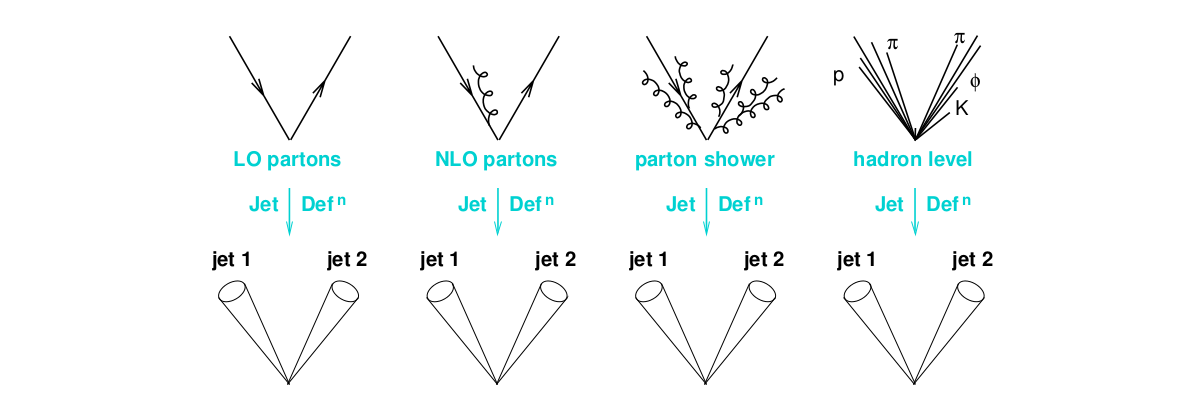
\includegraphics[width=1\textwidth]{Fig2/jetdefinition.png}
    \caption{The application of a jet definition to a variety of events that differ just through soft/collinear branching and hadronization should give identical jets in all cases~\cite{GavinLectures}.}
    \label{fig:jetdefinition}
  \end{center}
\end{figure}

Tradiontally, jet algorithms have been classified into two categories: cone algorithms and sequential recombination algorithms. 

Cone-like algorithms are based on the collinear nature of gluon radiation and the parton shower described above. The decay products of and emission from a hard quark or gluon will tend to form a cone of particles in the $\eta - \phi$ plane as they propagate.
% Then a cone of a suitable radius will capture these decay procuts.
An cone algorithm will work as follows~\footnote{This is how CMS cone algorithm, used for the preparation for the LHC running, works.}: first, it sorts all particles in the event according to their momentum, and identifies the one with largest $\pt$. This is referred to as seed particle. Then a cone of radius $R$ in  $\eta - \phi$ is drawn around the seed. The direction of the sum of the momenta of those particles is identified and if it doesn't coincide with the seed direction then the sum is used as a new seed direction, and iterates until the sum of the cone contents coincides withthe previus seed (this type of algorithm is cone ``iterative'' cone since it iterates the cone direction). This is how a stable cone is reached. A difficulty and major drawback in this procedure is the use of the transverse momentum of the particle to select the first seed. This definition is collinear unsafe, i.e. a splitting of the hardest particle into a nearly collinear pair can have the consequence that another, less hard particle, pointing in a different direction suddenly becomes the hardest in the event, leading to a different final set of jets. There are many other variants of cone algorithms, and nearly all suffer from problems of either collinear safety, or infrared safety (an extra soft particle creates a new seed, which can lead to an extra stable cone being found). A fix for these problems came in a algorithm called Seedless Infrared Safe Cone (SISCOne)~\cite{SISCone}.


Recombination algorithms, on the other hand, are both collinear and infrared safe. And for this reason, they can be used in calculations to any order in perturbation theory. The term recombination is used given that these algorithms work as if they were inverting the sequence of splittings of the parton shower. In general, recombination algorithms operate by successively combining pairs of particles using a distance metric, $d_{ij}$.  At hadron colliders, due to the fact that one of the incoming partons may continue along the beam, for every pair of particles this metric is compared to a so-called ``beam distance'', $d_{iB}$, and only when  $d_{ij}<d_{iB}$ the particle pair is combined and considered for subsequent clustering steps. 

ATLAS (and also CMS) has chosen anti-$k_t$~\cite{antiktalg} algorithm as the default jet algorithm for use in physics analysis.  This recombination algorithm as well as the Cambridge-Achen algorithm~\cite{CamAchen}, or C$/$A are extensions of the original $k_t$ algorithm developed for the analysis of multi-jet events at $e^+ e^-$ colliders~\cite{JADE} and subsequently extended for use at hadron colliders~\cite{kt2}~\cite{kt1}. In this thesis, the $k_t$ algorithm was used for jet substructure studies, see section~\ref{sec:substructure}.

The orginal $k_t$ algorithm implements the following (\ref{eqn:origkt}) distance metric between particles $i$ and $j$,

\begin{equation} 
d_{ij} = \frac{2E_i E_j (1-cos\theta_{ij}) }{Q^2}
\label{eqn:origkt}
\end{equation}

where $Q$ is the total energy in the event, $E_i$ is the energy of particle $i$ and $\theta_{ij}$ the angle between particles $i$ and $j$. In the collinear limit, $d_{ij}$ is related to the relative transverse momentum between particles $i$ and $j$ (hence the name $k_t$ algorithm), normalized to the total visible energy.
The particles are combined if the minimum $d_{ij}$, $d_min$, is below a certain threshold, $y_{cut}$.  The jet multiplicity depends on the value of $y_{cut}$, as a lower value will result in more soft or colliinear emissions surviving as jets. %This is thus the first definition of an ``event shape'', this threshold marks the transition between two-jet events and three-jet events.
As mentioned above, for hadron colliders, the notion of a beam distance is added. A distance scale, $\Delta R = \sqrt{\Delta y^2 +\Delta \phi^2}$, is introduced to define the typical radius for a jet, effectively replacing $y_{cut}$. In this case for every pair of particles a new distance is define, (\ref{eqn:kt}),

\begin{equation} 
d_{ij} = min(p^2_{ti},p^2_{tj}) \frac{\Delta R^2_{ij}}{R^2}
\label{eqn:kt}
\end{equation}

and the beam distance, $d_{iB}=p^2_{ti}$. %, in the way that when no particle j is found such that $\Delta R_{ij} < R$ then i is promoted to the status of a jet. 
The algorithm proceeds by searaching for the smallest of the $d_{ij}$ and the $d_{iB}$. If it is a $d_{ij}$ then particles $i$ and $j$ are recombined into a single new particles. If it is a $d_{iB}$ then $i$ is removed from the list of particles, and called a jet. This is repeated until no particles remain.

As opposed to cone algorithms, for the $k_t$ algorithm, the jets have quite irregular shapes, and particles with $\Delta R_{ij} > R$ can still be clustered within the jet. This is a problem when, for example, an irregularly shaped jet happens to extend into poorly instrumented detector regions. Another drawback of this definition is that soft particles are clustered first. This  has the potential to introduce complications when the detector noise of energy density fluctuations are large.

A feature of the $k_t$ algorithm that is attractive is that it not produces jets but also assigns a clustering sequence to the particles within the jet. It is possible then to undo the clustering and look inside the structure of the jet. This has been exploited in a range of QCD studies, and also in searches of hadronic decays of boosted massive particles  and will be used here for the search of two-pronged jets in gluon splitting.

The prescription above may be generalized beyond the $k_t$ algorithm. By inverting the power law in the particle distance metric, $d_{ij}$, the anti-$k_t$ algorithm is obtained. The particle distance metric used by this algorithm is,

\begin{equation} 
d_{ij} = min(p^{-2}_{ti},p^{-2}_{tj}) \frac{\Delta R^2_{ij}}{R^2}
\label{eqn:antikt}
\end{equation}

and the  beam distance, $d_{iB}=p^{-2}_{ti}$. This definition results in the clustering of the hardest emissions first. This has several benefits in the context of high-luminosity hadron collisions.

Note that the anti-$k_t$ algorithm does not provide useful information on jet substructure if a jet contains two hard cores, then the $k_t$ (or C/A) algorithms first reconstruct those hard cores and merge the resulting two subjets. The anti-$k_t$ will often first cluster the harder of the two cores and then gradually aglomerate the contents of the second hard core.

These algorithms, and more, are implemented in {\sc Fastjet}~\cite{fastjet} software package for jet-finding. 


%------------------------------------------------------------------------
\subsection{Jet substructure}\label{sec:substructure}
%------------------------------------------------------------------------

The study of a quantity related to the distributions and multiplicity of particles in the event phase space lead to the first evidence of jet structure, as pointed out in ref.~\cite{PhysRevLett.35.1609}. In general, all final hadronic states in $pp/p\bar{p}/e^+e^-$ collisions can be explored in terms of the structure and shape of the event energy flow by means of so called ``event shape'' variables. This family of variables attempt to extract information about the global geometry of an event, usually distinguishing between di-jet events and multijet final states. Such variables have been successfully utilized in many SM measurements and BSM searches, see for example~\cite{Abbiendi:2007aa}\cite{Aad:2012np}. 

Although very useful, event shape variables are not sensitive to the detailed structure and distribution of energy inside a particular jet in the event. In new physics searches, tools for the identification of individual objects that might be signature of new particles are desired. For example, when an unstable particle with large transverse momentum decays hadronically, the final state may contain a number of nearly collinear jets. These jets may be merged by a jet finder; %The decay products of boosted heavy quarks or bosons might be reconstructed as a single jet, 
a method for selecting these jets would allow for the study of their properties.
  This interest lead to the development of a wide range of jet substructure techniques in the recent years.

  Jet substructure methods probe the internal structure of jets from a detailed study of its constituents (see chapter\ref{sec:reconstruction}). These techniques have been first thought for distinguishing boosted hadronic objects from the background of jets initiated by light quarks and gluon, see for example~\cite{ATLASBoostedHbb},
%http://cdsweb.cern.ch/record/1201444/
but they have been also used succesfully in other applications, including separating quark jets from gluon jets~\cite{PhysRevLett.107.172001} and identifying boosted decay producs in new physics~\cite{PhysRevD.82.095012}.

%Jet shapes and jet algorithms in SCET, by Ellis, Vermillon, et all
Jet shapes, which are event shape-like observables applied to single jets, are an effective tool to measure the structure of individual jets~\cite{springerlink:10.1007/JHEP11(2010)101}.% {\bm ELEGIR REFERENCIA}. 
 The shape of a jet no only depends on the type of parton (quark or gluon) but is also sensitive to non-perturbative fragmentation effects and underlying event contributions~\cite{ATLASJetShapes}.


%from Jet substructure at the Tevatron and LHC
%Observables desinged to be sensitive to the internal structure of jets are expected to also be sensitive to pile-up. Large-radius jets, such as those used in the measurements of jet substructure, are naturally more susceptile to pile-up due to their larger catchment area~\cite{CatchmentArea}; the invariant mass of these large jets is particularly affected. %http://arxiv.org/abs/1009.1143
%Techniques for correcting these effects or mitigating their impact $-$such as the splitting and filtering procedure pioneered in ATLAS$-$  are essential in producing precision measurements for several of the analyses presented by the Tevatron and LHC experiments.  A more thorough review of these issues at ATLAS can be found in~\cite{DavidMillerThesis}


In the particular case of the present analysis, several distinguishing characteristics between jets originating from $b$-quarks and jets originating from the the splitting of a gluon into a $b\bar{b}$ pair can be determined using the techniques of jet substructure. 


\subsubsection{Jet width}


%From http://www.springerlink.com/content/54748j617818718q/?MUD=MP
The jet width is part of a set of continuous variables that try to distinguish individual particles/subjets within the jet as a smooth funcion of $(\delta \eta, \delta \phi)$ away from the jet axis, in order to form combinations like geometric moments.  This particular combination sums the distances between the jet constituents and its axes, weighted by the constituent $\pt$, and then normalized to the total $\pt$ of the jet. The compact definition is 

%\begin{equation} 
%g = \sum_{i\in jet} \frac{p^i_T}{p^{jet}_T} |\Delta R_i|
%\label{eqn:girth}
%\end{equation}
%where $\Delta R_i = \sqrt{\Delta y^2_i + \Delta \phi^2_i}$

\begin{equation} 
\mbox{ {\it Jet width}} = \frac{\sum_{i=1}^N \pt^{const_i} \,\Delta R (const_i,jet) }{\sum_{i=1}^N \pt^{const_i} }
\label{eqn:trackjetwidth}
\end{equation} 
where $N$ is the total number of calorimeter or track constituents.  This observable is also highly correlated to the mass of the jet.

This linear radial moment is a measure of the width or ``girth''~\cite{PhysRevLett.105.022001} of the jet.  Under the assumption of central jets with massless constituents at small angles, this linear moment is identical to jet broadening~\cite{Catani1992269}, defined as the sum of momenta transverse to the jet axis normalized by the sum of momenta. While jet broadening is natural at an $e^+ e^-$ collider, the linear radial moment is more natural at the LHC.

An alternative approach to measuring the width is to use the angular separation of the two hardest constituents inside jets. This has the advantage of effectively removing any dependence on the shower development within the calorimeter and focuses on the hard component of the jet.



%Measurement of QCD jet broadening~\cite{PhysRevD.44.601}.In this paper, we discuss the use of an event-shape parameter QT introduced by Ellis and Webber to describe hadronic final states in proton-antiproton collisions [18]. QT is defined as the scalar sum of the momenta perpendicular to the transverse thrust axis, where the transverse thrust axis represents the direction of maximum energy flow in the plane transverse to the beam. It has the property of being both finite and calculable for all multiparton final-state configurations, the case where particularly singularities occur in perturbation theory associated with the collinear emission of gluons. The behavior of QT with increasing energy is termed jet broadening because of its sensitivity to the increasing multiparton nature of a jet as the energy of the jet increases. % $Q_T / E_T$ ~ similar behavior with $E_T$ as Jet Width.

%Jet Angularities~\cite{springerlink:10.1007/JHEP11(2010)101} are also radial moments, but their “radial distances” are rescaled into the angular coordinates appropriate for $e^+ e^−$ event shapes. 



\subsubsection{Eccentricity}

In defining a jet moment there are several ways to weight the momentum and define the center of the jet. We have defined the jet width as the first moment of the transverse energy with respect to the jet axis; another example of useful combination is the jet pull~\cite{PhysRevLett.105.022001}. But it is also natural to look at higher moments, such as those contained in the covariance tensor,

\[ C = \sum_{i\in jet}\frac{p^i_T|r_i|}{p^{jet}_T} \left( \begin{array}{cc}
 \Delta y^2_i & \Delta y_i \Delta\phi_i \\ 
 \Delta\phi_i \Deltay_i & \Delta \phi^2_i \end{array} \right). \]


Here, $\vect{r}_i = (\Delta y_i, \Delta \phi_i) = \vect{c}_i - \vect{J}$, where $\vect{J} = (y_J,\phi_J)$ is the location of the jet and $\vect{c}_i$ is the position of a cell or particle with transverse momentum $p^i_T$. The eigenvalues $a \geq b$ of this tensor are similar to the semimajor and semiminor axes of an elliptical jet. The jet eccentricity, defined below, is a combination of these eigenvalues, and it is a measure of how elongated is the area of a jet.

\begin{equation} 
e = \sqrt{\frac{(a^2 - b^2)}{a}}
\label{eqn:ecc}
\end{equation}

%No significan difference in eccentricity was found between quark and gluon jets.


\subsubsection{Jet Mass}


The jet mass, like the linear radial moment, also depends on the radiation pattern of the event. It is the most basic observable for disinguishing massive boosted objects from jets originating from quarks or gluons. The latter are expected to be dominated by wide-angle emissions, with increase probability to see high mass jets initiated from gluons as opposed to quarks~\cite{PhysRevD.79.074012}.  


{\sc Need to complete this}.


%In the recent ATLAS analysis of 35~pb$^{-1}$ of data, the sensitivity of individual jet mass to pile-up is directly tested (for jets with at least 300~GeV). The mean jet mass is observed to increase linearly with NPV~\cite{ATLAS-CONF-2011-073}. %The filtering procedure significantly reduces the effect of pile-up on jet mass.




\subsubsection{Subjet multiplicity}

With the development of the $k_t$ algorithm, subjets were first used in the description of the hadronic final state in $e^+e^-$ annihilation, such as the study of the jet multiplicity at different energy scales~\cite{Catani1992445}. By using the sequential recombination algorithms introduced in the previus section, it is straightforward to define a ``subjet algorithm'' in which the structure of the jet's constituents is resolved using either the same jet finder algorithm or a new one with a fixed (smaller) distance parameter.

The subjet multiplicity $-$ the number of subjets within a jet $-$ provides information on the distribution of energy and multiplicity of particles within a jet. For instance, in~\cite{Snihur1999494} the result of meassuring this ``radiation variable'' on quark- and gluon-initiated jets indicates that gluon-initiated jets tend to have on average higher subjet multiplicity. This result is consistent with the QCD prediction that gluons radiate more than quarks. In the case of this and different other analyses % see for instance  http://iopscience.iop.org/1126-6708/1999/09/009/
the $k_t$ algorithm is rerun for subjet finding.

As an alternative to fixed distance parameter subjets, it is also possible to undo the last step in the recombination sequence~\cite{kt2} in order to identify the decay products of an object.  This approach is used in seveal jet grooming procedures\footnote{Jet grooming comprises dedicated techniques to remove uncorrelated radiation within a jet. A review of these procedures can be found in~\cite{Abdesselam:2010pt}. }, see for instance~\cite{pruning}.

%In contrast to the $k_t$ algorithm, it is not useful just to undo the last stage of C/A clustering: The absence of any momentum scale in its distance measure means that the last clustering often involves soft radiation on the edges of the jet and so, is unrelated to the heavy object's decay. 
%The so-called BDRS method of jet grooming
%http://prl.aps.org/abstract/PRL/v100/i24/e242001
% uses the C/A algorithm. Subjets are then defined by de-clustering the C/A algorithm and evaluating the relative mass of the subjets compared to the parent jet. As a final step, the three hardest identified subjets are recombined to define the resulting ``filtered'' jet.

It is also possible to extend the use of individual subjets in conjunction with more traditional jet shape variables. Using these tools, an inclusive jet shape based on the substructure topology of a single jet, ``$N$-subjettiness''~\cite{nsubjettiness} is defined.





\subsubsection{$N$-subjettiness}

As mentioned above, the $N$-subjettiness~\cite{nsubjettiness} is a jet shape that describes the energy flow within a jet. It quantifies the degree to which  radiation is aligned along specified subjet axes. This jet shape was adapted from the event shape $N$-jettiness~\cite{njetti}.

Given candidate subjets directions determined by an external algorithm such as the exclusive $k_t$ procedure~\cite{exclusivekt}, the variables is defined as,


\begin{equation} 
\tau^{(\beta)}_N = \frac{1}{\sum_k {\pt}_k\,(R_0)^{\beta}} \sum_k {\pt}_k (\min \{ \Delta R_{j1,k},\,\Delta R_{j2,k},...,\,\Delta R_{jN,k} \})^{\beta}
\label{eqn:nsubjet}
\end{equation} 

The sum runs over the $k$ constituent particles in a given jet where $p_{T,k}$ are their transverse momenta, and $\Delta R_{j1,k}$ is the distance between the candidate subjet $j1$ and a constituent particle $k$.  $R_0$ is the characteristic jet radius used in the original jet clustering algorithm.
The exponential weight, $\beta$, can optionally be applied to the angular distance computed between the subjets and the jet constituents.  

This jet shape was designed to identify boosted $N$-prong hadronic decays. With $\beta=1$, the definition above indicates that jets with $\tau_N\approx 0$ have all their radiation aligned with the candidate subjet directions and therefore have $N$ (or fewer) subjets. Jets with $\tau_N\gg 0$ have a large fraction of their energy distributed away from the candidate subjet direction and therefore have at least $N+1$ subjets.

To separate boosted hadronic objects from the QCD jet background, one could use the complete set of  $\tau_N$ (with different values of $\beta$) in a multivariate analysis. However, \cite{nsubjettiness} showed that a simple cut on the ratio $\tau_N/\tau_{N-1}$ provides excellent discrimination power for $N$-prong hadronic objects. In particular, $\tau_2/\tau_1$ can identify boosted $W/Z$ and Higgs bosons, with the angular weighting exponent $\beta =1$ providing the best discrimination.

Since eq.~\ref{eqn:nsubjet} is linear in each of the constituent particle momenta, this variable is an infrared- and colliner-safe observable.  In subsequent work~\cite{mininsubjettiness}, Thaler and van Tilburg showed that the initial step of choosing candidate subjet axes is in fact unnecessary. In particular, the quantity in equation~\ref{eqn:nsubjet} can be minimised over the candidate subjet directions, further improving boosted object discrimination.

The definition of $N$-subjettiness is not unique, and different choises can be sued to give different weights to the emissions within a jet. There generalizations of $N$-subjettiness are similar to different ``angularities''~\cite{angularities} used in $e^+e^- \rightarrow$hadrons measurements.


%From Nsubjettiness paper
%use $N$-subjettiness to effectively ``count'' the number of subjets in a jet. Compare to previous jet substructure techniques, $N$-subjettiness  has the advantage of finding jets that contain two or more lobes of energy.
%Subjet candidates where determined by using the exclusive $k_t$ algorithm, forcing it to return exactly $N$ jets.


 
%%
%%%%%%%%%%%%%%%%%%%%%%%%%%%%%%%%%%%%%%%%%%%%%%%%%%%%%%%%%%%%%%%%%%%%%%%%%%%%%%%
% The LHC
%%%%%%%%%%%%%%%%%%%%%%%%%%%%%%%%%%%%%%%%%%%%%%%%%%%%%%%%%%%%%%%%%%%%%%%%%%%%%%%
%
\chapter{The ATLAS detector at the LHC}

\section{The Large Hadron Collider}


The Large Hadron Collider  (LHC)~\cite{Breskin:1244506} is a proton-proton ($pp$) synchrotron located in the previous Large Electron Positron (LEP) collider tunnel at CERN Laboratory, just outside the city of Geneva (Switzerland), approximately 100~m underground. It is designed to collide bunches of up to $\sim 10^{11}$ protons every 25~ns at a center-of-mass energy of 14~TeV (seven times the 2~TeV reached by the Tevatron accelerator at Fermilab Laboratory, in Chicago). 

The experiments analyzing the collisions produced by the LHC are distributed around the 27~km ring at the various interaction points. The ATLAS experiment is located at Point 1, which is closest to the main CERN site. Point 5 houses the other general purpose detector, CMS. ALICE and LHCb experiments are located at Point 2 and Point 8, respectively. The former is designed to investigate heavy ion collisions; the latter, to investigate rare decays of b-mesons. The layout of these four experiments along the LHC ring is shown in Fig.~\ref{fig:LHC1}.

\begin{figure}[htbp]
  \begin{center}
      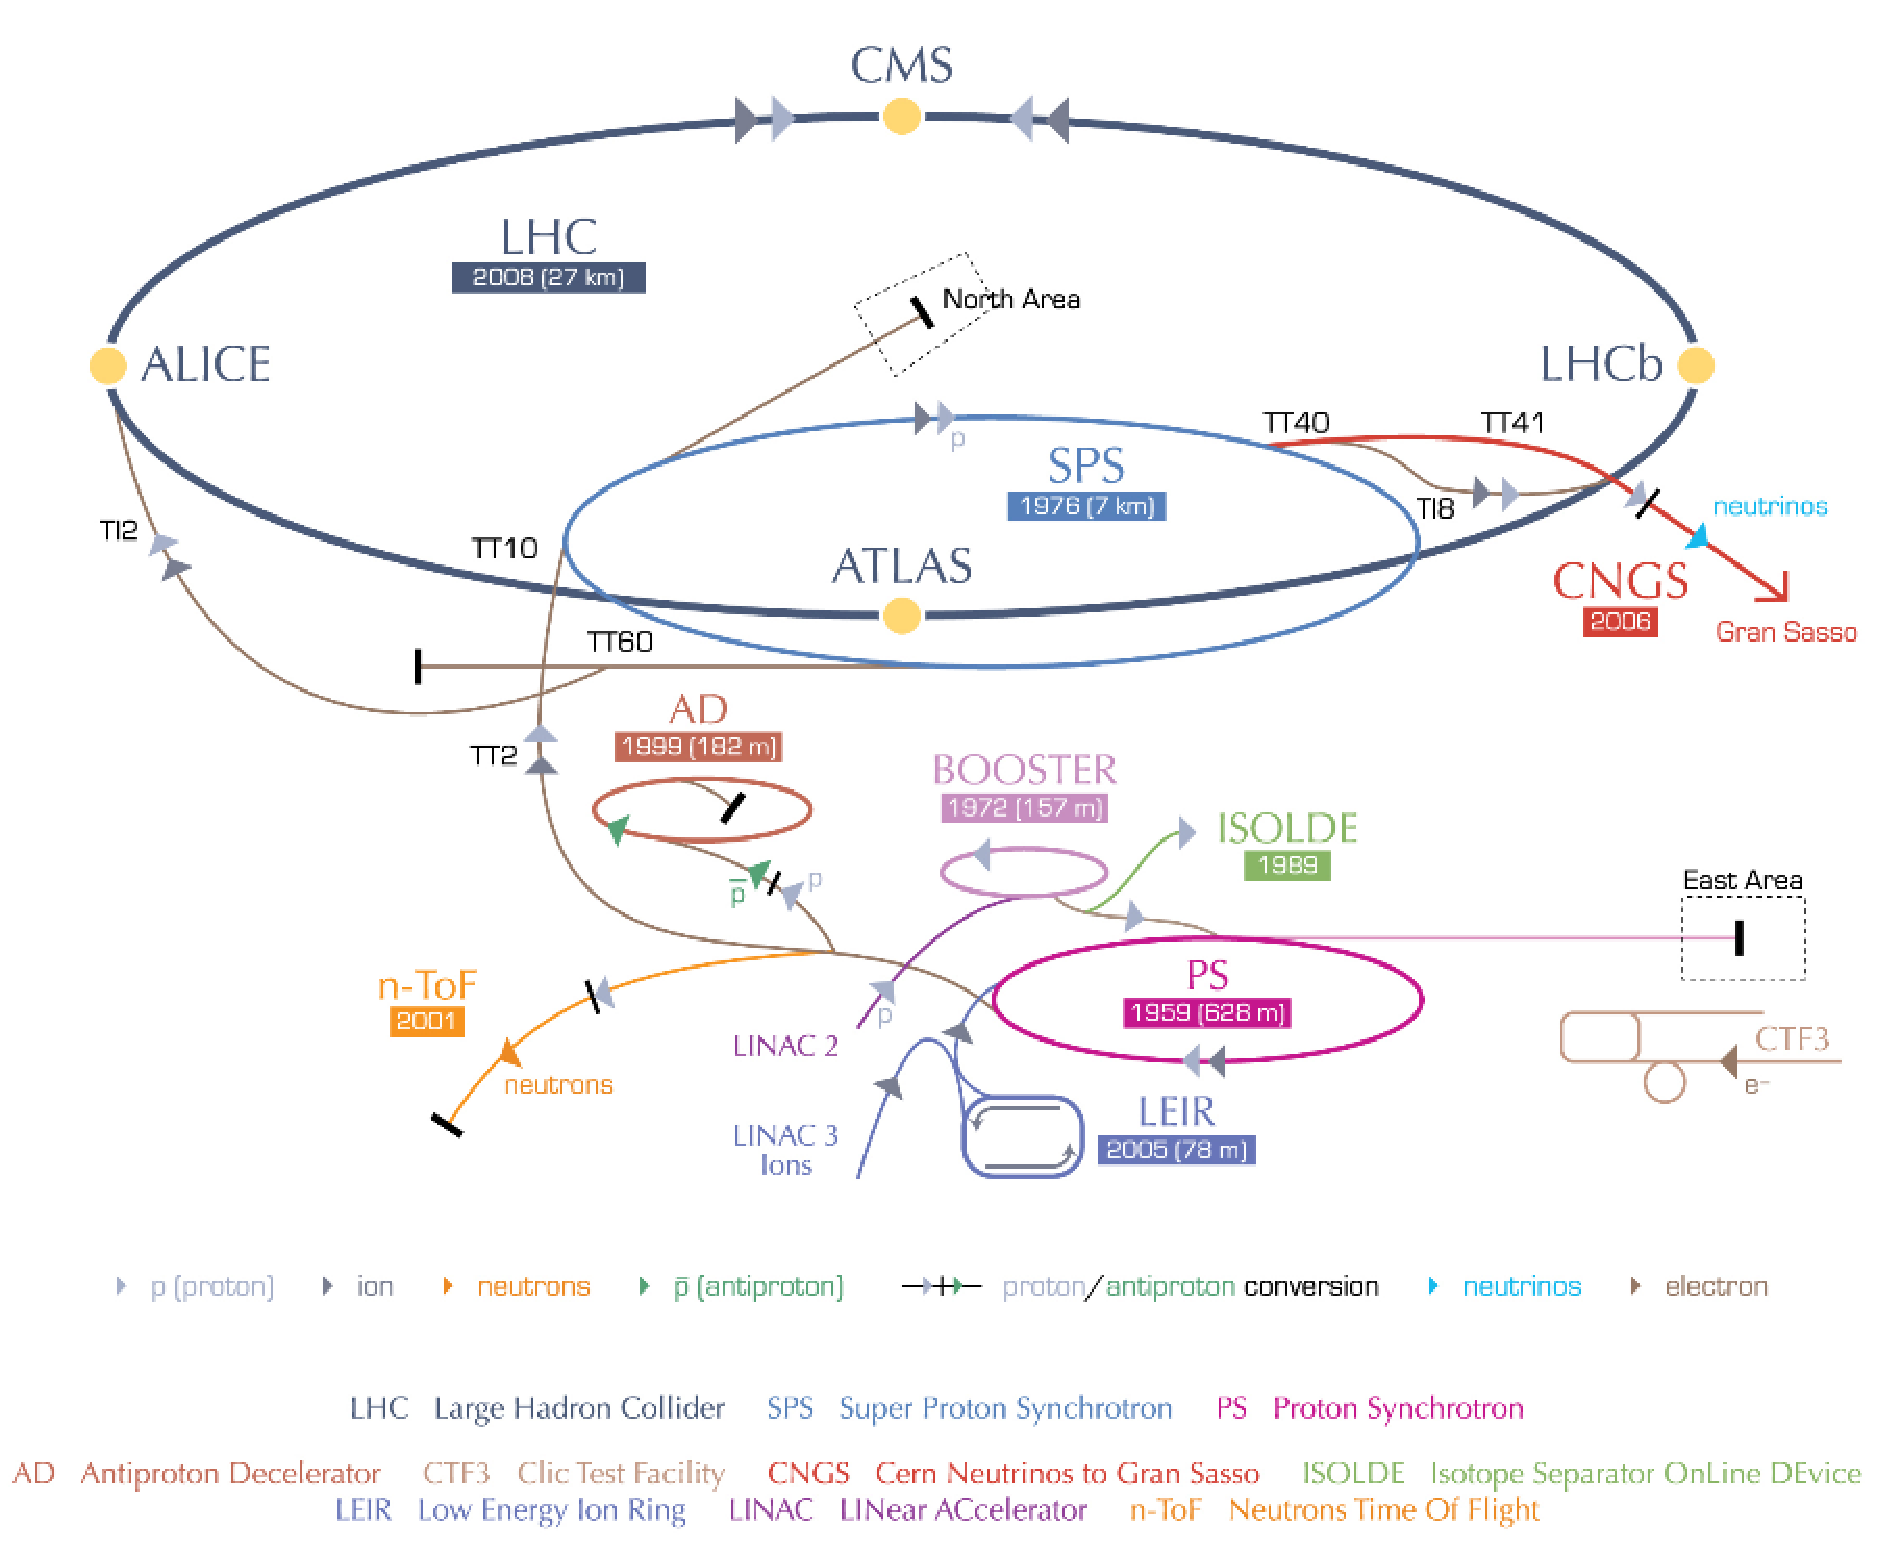
\includegraphics[width=1\textwidth]{Fig2/CERNacceleratorcomplexCut.pdf}
    \caption{The CERN accelerator complex, showing the injection system, along with each component’s date of construction, and the placement of the four main experiments.}
    \label{fig:LHC1}
  \end{center}
\end{figure}


Proton beams are formed, before insertion into the main LHC ring, using a succession of smaller machines with increasingly  higher energies, as shown in Fig.~\ref{fig:LHC1}. The chain begins as protons are injected into the PS Booster (PSB) at an energy of 50~MeV from Linac2. The booster accelerates them to 1.4~GeV. The beam is then fed to the Proton Synchroton (PS) where it is accelerated to 25~GeV. At desin strength, the bunch structure, known as a bunch train, contains 72 bunches of protons upon entry to the Super Proton Synchrotron (SPS). The SPS accumulates up to four fills of 72 bunches from the PS and accelerates them to 450~GeV, with a bunch spacing of $\sim$~25~ns. They are finally transferred to the LHC (both in a clockwise and an anticlockwise direction) where they are accelerated for 20 minutes to their nominal energy of 7 TeV. Beams will circulate for many hours inside the LHC beam pipes under normal operating conditions.

The bunch structure is a direct consequence of a radio frequency (RF) acceleration scheme used to attain the desired high proton beam energy.  In RF acceleration, particles travel through a series of time-varying electrical fields and they can only be accelerated when the RF field has the correct orientation when particles pass through an accelerating cavity, which happens at well specified moments during an RF cycle. The result of a sequence of RF accelerations is several bunches of protons. It is important to note that when we speak about ``beams'' we refer to many bunches of protons separated by some uniform distance. Increasing the number of bunches is one of the ways to increase luminosity in a machine (more about luminosity in subsection~\ref{sec:lumiintro}). At desinged beam intensitity, when the bunches cross, there will be a maximum of about 20 collisions.

A larged magnetic field is needed to guide and maintain the beam particles in their circular orbit. The needed field is achieved using superconducting electromagnets built from NbTi coils that operate in a superconducting state, efficiently conducting electricity without resistance or loss of energy. The currents through the coils produce magnetic fiedls perpendicular to the direction of motion of the protons that deflect the protons into their orbits.  The whole magnetic system comprises 1232 dipole magnets of 15~m length which are used to bend the beams, and 392 quadrupole magnets, each 5–7~m long, to focus the beams. At a peak beam energy of 7~TeV, the dipoles need to produce an 8.33~T magnetic field, requiring a current of $\sim$ 12~kA. In order to deliver the current densities and magnetic field required for 7~TeV proton beams, the magnets are kept at 1.9~K by circulating superfluid helium.

The first $pp$ collisions produced by the LHC ocurred on November 23 2009, at the SPS extraction energy of 450~GeV per beam. Very quick after, on December 8, ATLAS and CMS detectors started recording data at energy of 2.36~TeV. By this time the LHC became the highest energy accelerator in the world.  During this period, bunch intensities were limited by machine-protection considerations to 1.5 $\times$ 10$^{10}$ protons.

 In February 2010, the LHC was commissioned once more with 450 GeV beams, and a series of tests were performed to ensure that the magnet systems could operate safely at the currents necessary to control 3.5 TeV beams. This was followed by the very first collisions at 7~TeV center-of-mass energy on March 30. During the 2010 run the beam parameters were tuned (the beam widths squeezed and the number of protons per bunch and the number of bunches in each beam increased) in order to increase the beam intensity.  In particular, as the intensity of the beams increased, the mean number of interactions per bunch crossing increased.  


Finally, the data samples analysed in this thesis correspond to proton-proton collisions at $\sqrt{s}=7$ TeV delivered by the LHC and recorded by ATLAS between May and November 2011, with the LHC running with 50~ns bunch spacing. Table~\ref{tab:beamparameters} summarizes the basic beam parameters expected for design energy and luminosity and the beam parameters as of May 2011. The LHC performance steadily improved during 2011. The average number of interactions per bunch crossing throughout the data-taking period considered rapidly increased approximately from $\sim$3 to 8 until (northern hemisphere) summer 2011, with a global average for this period of $\approx 6$. Starting in August 2011 and lasting through the end of the proton run, this number ranged from approximately 5 to 17, with an average of about 12. This evolution is illustrated in Fig.~\ref{fig:peakAvgMu}, which shows the maximum mean number of collisions per beam crossing versus day in 2011. 


\begin{table}[!hbt] %[h]
\renewcommand{\arraystretch}{1.2}
\centering
\begin{tabular}{ | c | c | c |}
\hline
  ~~~~~~~~~~~~~~~~Parameter~~~~~~~~~~~~~~~~ &~~~~~~2011 runs~~~~~~ &~~Design~~ \\ \hline
  Center-of-mass energy [TeV]         &  7    & 14 \\ 
  Instantaneus luminosity [cm$^{-2}$s$^{-1}$]     & 3.65 10$^{33}$ (year peak)  & 10$^{34}$     \\ 
  Bunches per beam  &  38 (May)  & 2808        \\ 
  Protons per bunch &  0.8$\times$10$^{11}$ (May)   & 1.5$\times$10$^{11}$    \\
  Mean interactions per crossing  &  6 to 12 (year average) & 23        \\ \hline 
\end{tabular}
\caption{Summary of beam conditions during the 2011 7 TeV runs and those foreseen at design energy and luminosity.
}
\label{tb:beamparameters}
\end{table}


\begin{figure}[htbp]
  \begin{center}
      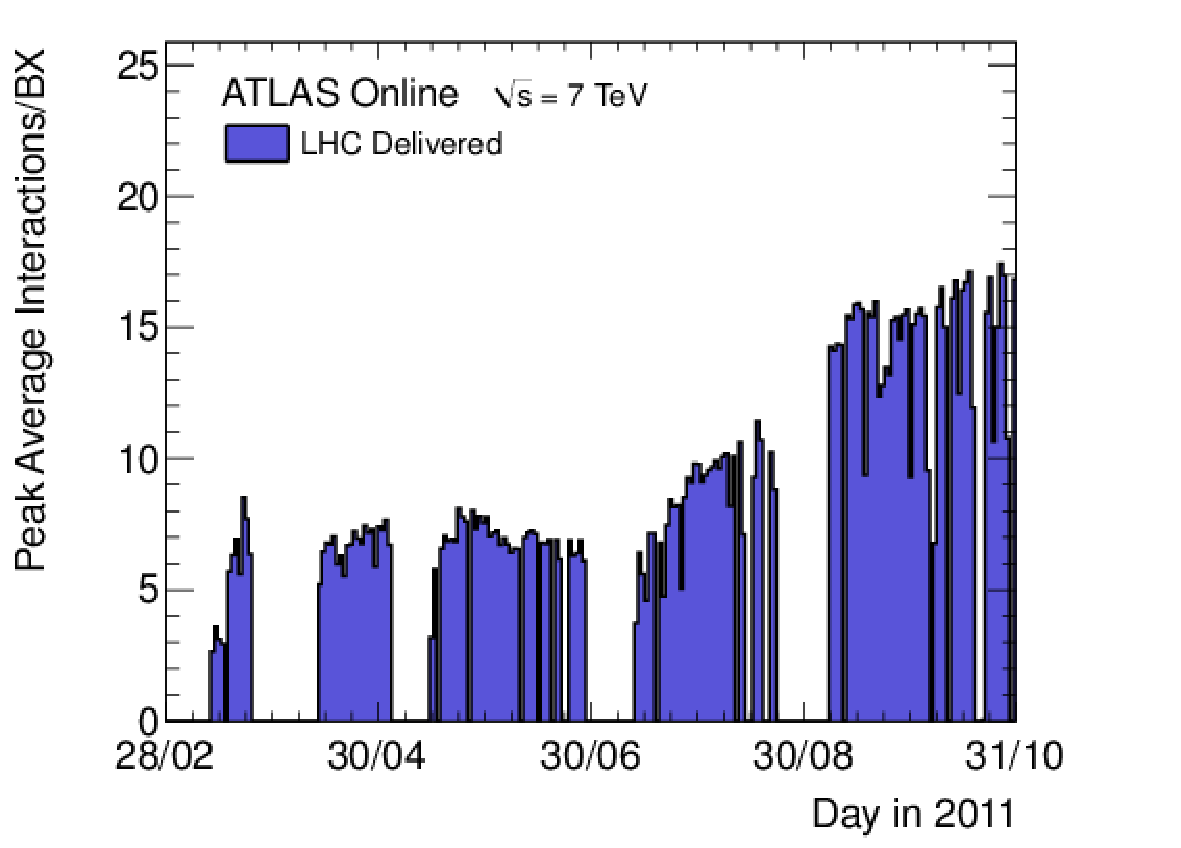
\includegraphics[width=0.7\textwidth]{Fig2/peakAvgMuByDay.pdf}
    \caption{The maximum mean number of events per beam crossing versus day in 2011.}
    \label{fig:peakAvgMu}
  \end{center}
\end{figure}


%------------------------------------------------------------------------
\subsection{Luminosity and pile-up}\label{sec:lumiintro}
%------------------------------------------------------------------------

The rate of events produced by the colliding beams depends on the luminosity of the collisions, which is a measure of the number of events per second per unit cross section, typically measured in units cm$^2$s$^{-1}$. The number of events of a particular process, then, is given by the product of the integrated luminosity, $\int dt L$, and the cross section of the process, $\sigma_{event}$.  The integrated luminosities are typically quoted in units of inverse picobarns, pb$^{-1}$~=~10$^{-36}$cm$^{2}$. In order to measure processes with very little cross sections a very high luminosity is required. 

The delivered luminosity can be written as~\cite{ATLAS-CONF-2011-116}:

\begin{equation} 
\mbox{ {\it L }} = \frac{n_b f_r n_1 n_2 }{2\pi \Sigma_x \Sigma_y}
\label{eqn:lumi}
\end{equation} 
where n$_b$ is the number of colliding bunch pairs,  n$_1$ and n$_2$ are the bunch populations (protons per bunch) in beam 1 and beam 2 respectively (together forming the bunch charged product), $f_r$ is the machine revolution frequency, and $\Sigma_x$ and $\Sigma_y$ are the width and the height of the proton beams. %characterize the horizontal and vertical profiles of the colliding beams. 

The number of protons per bunch, the number of bunches per beam, and the revolution frequency are all set by the beam operators. The widths of the proton beams are measured in a process known as a Van der Meer ($vdM$) scan~\cite{vanderMeer:296752}. In a $vdM$ scan, the beams are separated by steps of a known distance. The collision rate is measured as a function of this separation, and the width of a gaussian fit to the distributions yields the width of the beams in the direction of the separation.  

The total integrated luminosities provided by the LHC and recorded by ATLAS in 2011 are shown in Figure~\ref{fig:integratedlumi}. These events form the dataset analyzed in this thesis. By means of the beam-separation or $vdM$ scans, as well as other techniques to measure the bunch charged product, the ATLAS Collaboration has determined that the uncertainty on its luminosity measurement is $\delta L = \pm 3.7$\%. For a complete description of the methods used and the systematic erros evaluated see reference~\cite{ATLAS-CONF-2011-116}.

\begin{figure}[htbp]
  \begin{center}
      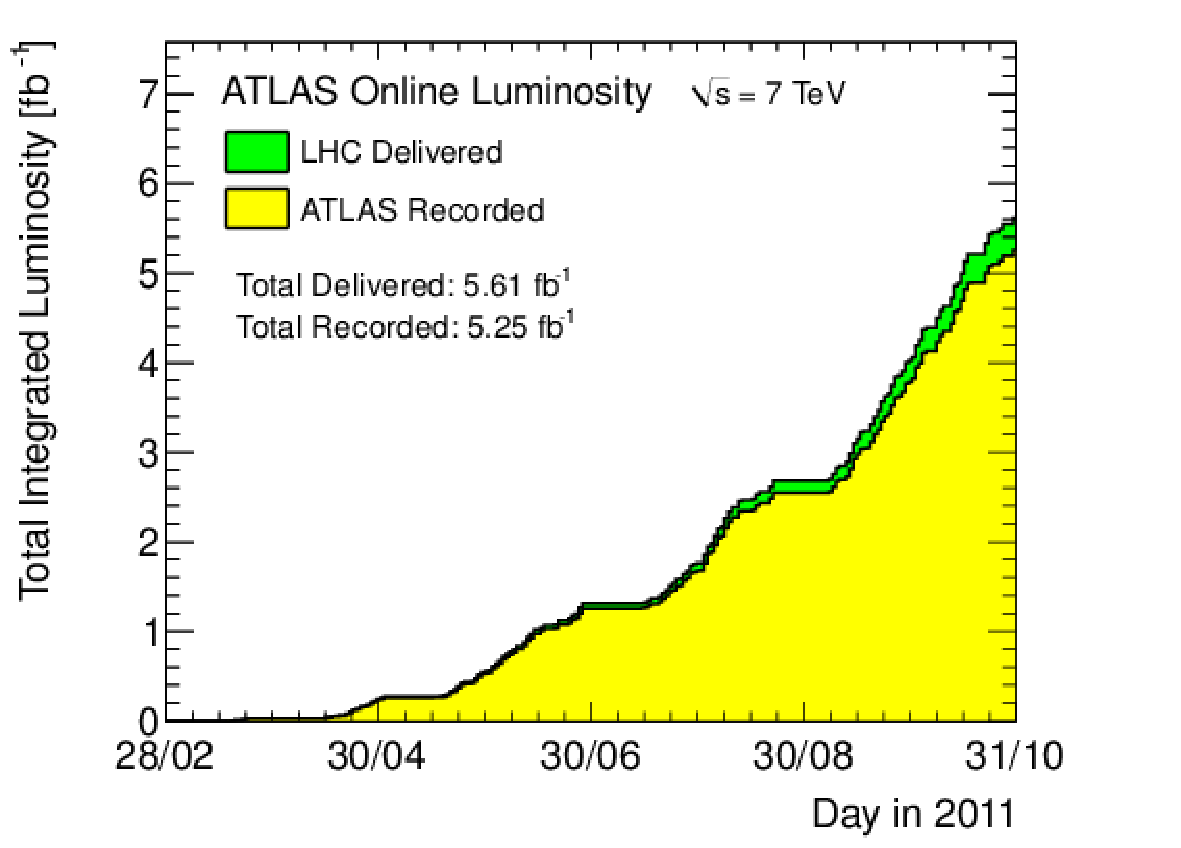
\includegraphics[width=0.7\textwidth]{Fig2/sumLumiByDay.pdf}
    \caption{Total luminosity delivered by the LHC and recorded by ATLAS during the 2011 $sqrt{s}$ = 7~TeV proton-proton run}
    \label{fig:integratedlumi}
  \end{center}
\end{figure}


As anticipated, due to the cross-section for interaction and the number of protons per bunch, the possibility to observe multiple $pp$ interactions per bunch crossing increases proportionally. This phenomenon, referred to as ``pile-up'', can really occur in two distinct forms. The first form is the presence of multiple $pp$ collisions (different from the interaction of interest) in the same bunch crossing, referred to as ``in-time'' pile-up. The second form of pile-up takes place due to electronic integration times within the detector. Certain detector components are actually sensitive to multiple bunch crossings due to the long electronic signals generated in the response to energy depositions or charge collection. One or more $pp$ collisions in a bunch-crossing different from that which produced the collision of interest can then affect the measurement. This form of pile-up is referred to as ``out-of-time'' pile-up and will become more and more important as the LHC bunch spacing gets closer to the nominal value, 25~ns.

The fraction of events with pile-up increased significatively since the data taking started. The experimental signature of this fact is obtain via the number of reconstructed primary vertices, or NPV. The effect of the event NPV is an important concern for the measurement of jet properties and will be discussed in the next chapters.


%
%%%%%%%%%%%%%%%%%%%%%%%%%%%%%%%%%%%%%%%%%%%%%%%%%%%%%%%%%%%%%%%%%%%%%%%%%%%%%%%
% ATLAS
%%%%%%%%%%%%%%%%%%%%%%%%%%%%%%%%%%%%%%%%%%%%%%%%%%%%%%%%%%%%%%%%%%%%%%%%%%%%%%%
%
\section{The ATLAS Detector}

%------------------------------------------------------------------------
%\subsection{Detector overview}\label{sec:atlassummary}
%------------------------------------------------------------------------

The ATLAS detector~\cite{ATLAS} is one of the two general purpose particle detectors built for probing $pp$ collisions at the LHC. As it was described in the previous section, inside the LHC, bunches of up to 10$^{11}$ protons will collide 40 million times per second to provide 14~TeV proton-proton collisions at a nominal luminosity of 10$^{34}$cm$^{-2}$s$^{-1}$. These high interaction rates and energies, as well as the requirements for high precision physics measurements set the standars for the design of the detector. At even 7 TeV center-of-mass energy, the LHC interactions result in high particle multiplicity, requiring fine detector granularity, and particle production at forward rapidity, requiring large detector angular coverage.

To achieve these performance goals, a design consisting of multiple detector sub-systems with cylindrical symmetry around the incoming beams is used as shown in Fig.~\ref{fig:ATLAS}. Closest to the interaction point the inner tracking detector is placed, providing charged particle reconstruction. The magnet configuration comprises a thin superconducting solenoid surrounding the inner detector cavity, and three large superconducting toroids (one barrel and two end-caps) arranged with an eight-fold azimuthal symmetry around the calorimeters. This fundamental choice has driven the design and size (44~m in length and 25~m in height) of the rest of the detector. Outside the solenoid, a calorimeter system performs electron, photon, tau, and jet energy measurements. Finally, the calorimeter is surrounded by the muon spectrometer where an array of muon drift chambers perform muon identification and momentum measurements.

The ATLAS detector coordinate system is used to describe the position of particles as they traverse these subdetectors. It is a right-handed coordinate system, with z pointing along the beam direction, positive x pointing toward the center of the LHC ring, and positive y pointing up. The x − y plane is referred to as the transverse plane, and the z direction as the longitudinal
direction. The azimuthal angle $\phi$ is measured as usual around the beam axis, and the polar angle $\theta$ is the angle from the beam axis. The pseudorapidity is defined as $\eta = − ln tan(\frac{\theta}{2})$, regions of low $\eta$ are referred to as ``central'', and regions of high $\eta$ are referred to as ``forward''. % (in the case of massive objects such as jets, the rapidity y = 1/2ln[(E + pz )/(E − pz )] is used). 
The transverse momentum $\pt$ is defined in the x-y plane unless stated otherwise. The distance $\Delta R$ in the pseudorapidity-azimuthal angle space is defined as $Delta R = \sqrt{ \Delta \eta^2  + \Delta \phi^2}$ .

\begin{figure}[htbp]
  \begin{center}
      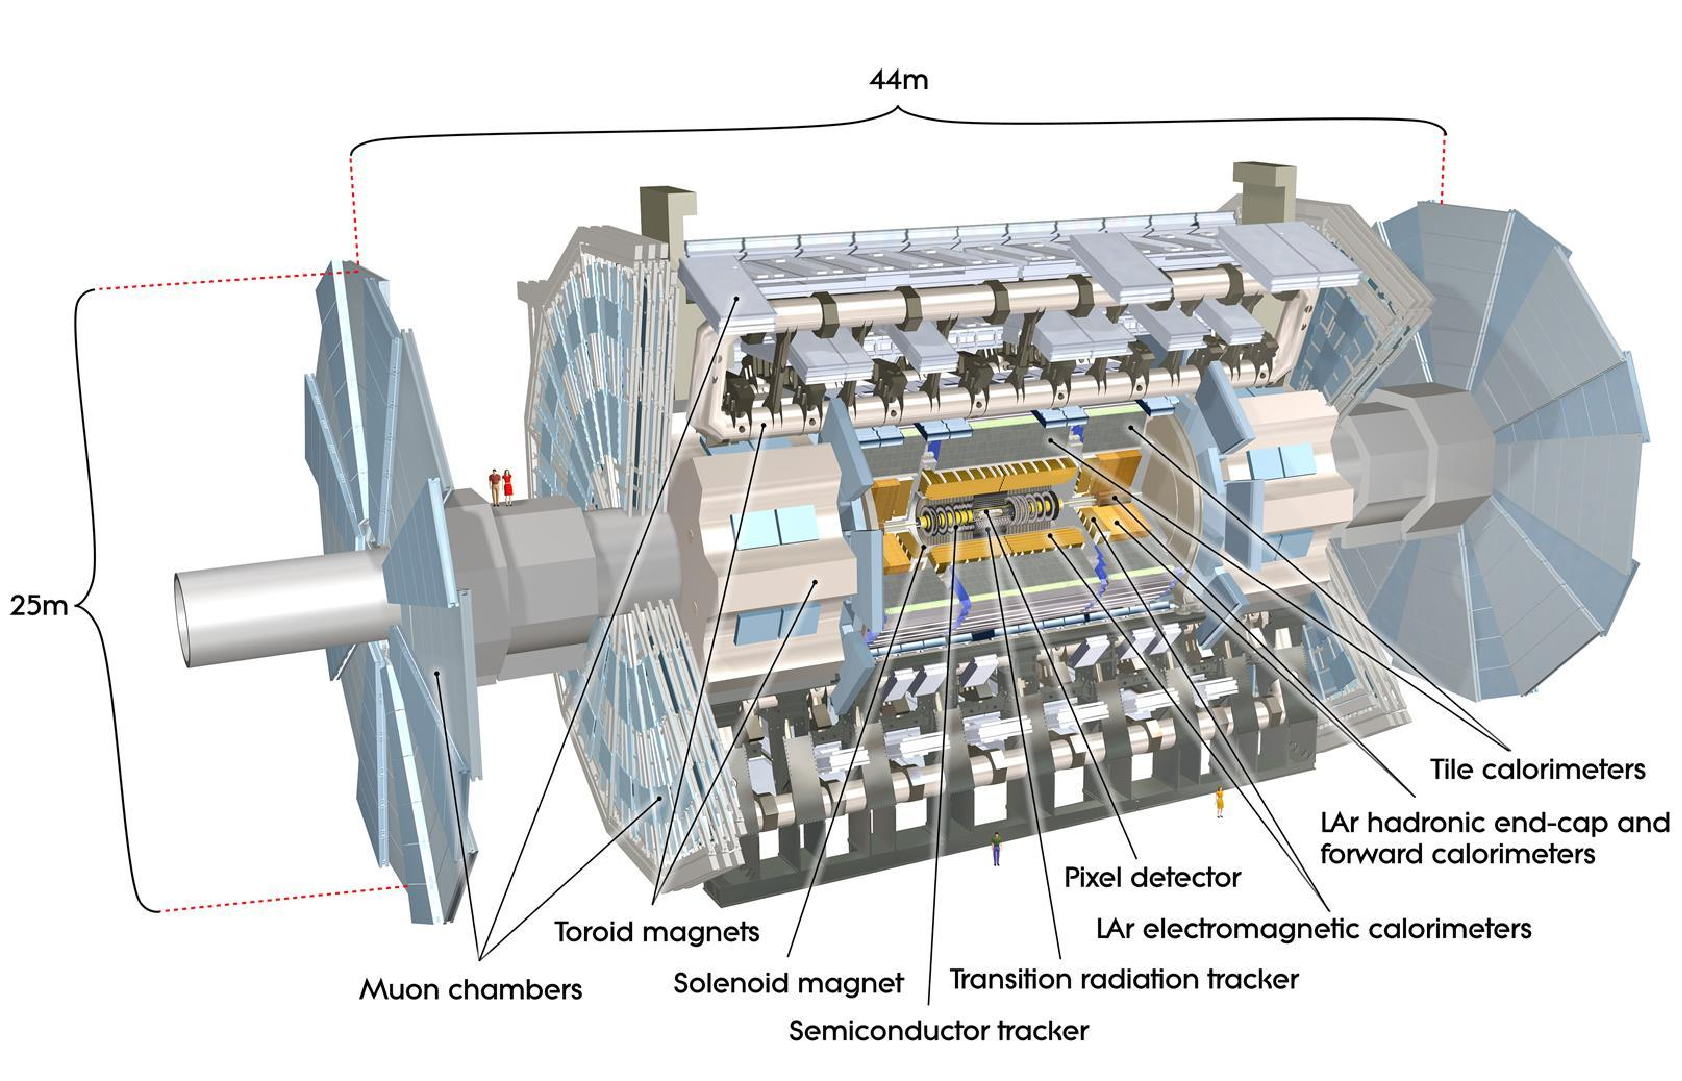
\includegraphics[width=0.9\textwidth]{Fig2/ATLASDetector.pdf}
    \caption{El detector de ATLAS}
    \label{fig:ATLAS}
  \end{center}
\end{figure}

To meet the extremely high demands that the LHC luminosity places on the speed with which ATLAS must record data, a dedicated trigger and data acquisition (TDAQ) systema is used. The interaction rate at the design luminosity is approximately 1~GHz, while the event data recording, based on technology and resource limitations, is limited to about$\sim$200~Hz. This requires a high rejection of minimum-bias processes while maintaining maximum efficiency for the new physics. The Level-1 (L1) trigger system uses a
subset of the total detector information to make a decision on whether or not to continue processing an event, reducing the data rate to approximately 75~kHz (limited by the bandwidth of the readout system, which is upgradeable to~100 kHz). The subsequent two levels, collectively known as the high-level trigger (HLT), are the Level-2 (L2) trigger and the event filter. They provide the reduction to a final data-taking rate of approximately 200 Hz. 



%------------------------------------------------------------------------
\subsection{Inner tracking system}\label{sec:atlasID}
%------------------------------------------------------------------------

The inner tracking system or inner detector (ID) is composed of three subdetectors: the pixel detector, the semiconductor tracker (SCT) and the transition radiation tracker (TRT). The goal of these three is to provide charged particle trajectory reconstruction and momentum measurements with an overall acceptance in pseudorapidity of $|\eta| < 2.5$ and full $\phi$ coverage. 

The sensors which built this system register signals, referred to as ``hits'', in response to the passage of charged particles. The ID is inmersed in a 2~T magnetic field, generated by the central solenoid. The positions of the registered hits are combined to form tracks, with the radius of curvature  of the tracks (caused by the presence of the magnetic field) providing a measurement of the particle’s transverse momentum. The track reconstruction efficiency ranges from 78\% at $p^{track}_{T} = 500$~MeV to more than 85\% above 10~GeV, averaged across the full $\eta$ coverage~\cite{chargemultiplicity}. The transverse momentum resolution of $\sigma_{p_T}$/$\pt$ = 0.05~\cite{ATLAS-CONF-2010-009} (upper bound) and a transverse impact parameter resolution of $\sim$20~ $\mu m$ for high momentum resolution particles in the central $\eta$ region\cite{ATLAS-CONF-2010-070}. 

The pixel detector, SCT, and TRT sensors are arranged on concentric cylinders around the beam axis, known as barrel layers, and on disks perpindicular to the beam at either end of the barrel, known as end-caps. A more complete description of these systems is given below. The overall layout of the inner detector is shown in Fig.~\ref{fig:figinner}. 


\begin{figure}[htbp]
  \begin{center}
      \includegraphics[width=0.9\textwidth]{Fig2/InnerDetector.pdf}
    \caption{Layout of the ATLAS inner detector.}
    \label{fig:figinner}
  \end{center}
\end{figure}


\subsubsection{The Pixel detector}

The pixel detector consists of three concentric barrel layers. The innermost one, the so called ``b-layer'' due to its role in identifying $b$-quarks initiated jets, is located at 5~cm from the interaction region. Three additional disks are located at each end-cap, producing typically three pixel position measurements per charged particle track.  Each layer or disk is instrumented with modules that form the basic unit of data acquisition, each with 47232 pixels.  All pixel sensors are identical and have a minimum pixel size in $r$ - $\phi \times z$ of 50 $\times$ 400~$\mu m^2$. The intrinsic accuracies in the barrel are 10 $\mu m$ in $r$ - $\phi$ and 115 $\mu m$ along $z$, or along $r$ in the end-caps. The pixel detector has approximately 80.4 million readout channels, an order of magnitude more readout channels than the rest of ATLAS combined, and it extends to a total length of $z \sim \pm$650~mm and radius of $r \sim$150~mm, providing good reconstruction efficiency for tracks up to $|\eta| <$2.5.

 
\subsubsection{The SCT}


The SCT consists of four barrel layers and nine end-cap layers surrounding the pixel detector, resulting in at least four hits along every charged particle track.  The SCT barrel reaches to $z\sim \pm$750~mm and $r \sim $515~mm, while the end-cap covers out to $z\sim \pm$2720~mm and $r =$560~mm.  There are 15,912 SCT module sensors, each 12.8~cm long and approximately 285~$\mu $m thick. 

In the barrel region, these modules use small-angle (40~mrad) stereo strips to measure both coordinates, with one set of strips in each layer parallel to the beam direction, measuring the $\phi$ coordinate directly . In the end-cap region, the detectors have a set of strips running radially and a set of stereo strips at an angle of 40~mrad. The mean pitch of the strips is 80~$\mu m$. The intrinsic accuracies per module in the barrel are 17~$\mu m$ in $r$ - $\phi $ and 580~$\mu m$ in $z$ (or $r$ in the end-caps). The total number of readout channels in the SCT is approximately 6.3 million.  A hit is registered only if the pulse height in a channel exceeds a preset threshold ($\sim $ 1~fC). The charged measured in the strip is then recorded into a memory buffer that is only read out and used for tracking if a trigger is received signaling that the event should be considered in more detail.


  
\subsubsection{The TRT}

The TRT surrounds the silicom detectors and is comprised of up to 76 layers of longitudinal straw tubes in the barrel, extending to $z\sim \pm$710~mm and $r \sim$1060~mm, and 160 radial straw planes in each end-cap cylinders, reaching $z\sim \pm$2710~mm and $r \sim$1000~mm.

 The TRT sensors are thin drift tubes consisting of cathode metal straws filled with an ionizing gas mixture of xenon, oxygen, and CO$_2$, with an anode wire running down the center of the straw. The passage of a charged particle through the gas produces positive ions and free electrons, which travel to the cathode and anode, respectively, under the influence of an applied voltage of 1600~V. Comparing the time that the signals are received at the cathode and the anode gives a drift time measurement that can be used to calculate the impact parameter of the particle. This method gives no information on the position along the length of the straw.

To give the best resolution of particle trajectories as they bend in the solenoidal field, the straws lie along the beam direction in the barrel and radially in the end-caps. The straw diameter of 4~mm causes a maximum drift time of approximately 48~ns and an intrinsic accuracy of 130 μm along the radius of the straw.

In addition to directly detecting charged particles produced by the collision, the TRT also measures the transition radiation induced by the passage of these particles through polypropylene sheets placed between the drift tube straws. Transition radiation refers to the photons emitted by charged particles as they pass from one material into another with a different dielectric constant. These photons yield a much larger signal amplitude than the charged particles, so separate thresholds in the electronics can be used to distinguish the two.

 
 % Este sistema de detecci\'on por tubos provee un gran n\'umero de puntos por traza (t\'ipicamente 36 puntos), lo cual determina un seguimiento cont\'inuo de la misma, con mucho menos material por punto y menor costo (mucho menor comparado con la tecnolog\'ia de p\'ixeles implementada en el subdetector m\'as interno).  La gran cantidad de puntos o impactos por traza es un instrumento poderoso en la b\'usqueda y reconstrucci\'on de trazas en el detector interno.

One of the most important tasks of the inner detector is to provide accurate collision vertex identification, exploiting the excellent position resolution and tracking efficiency. Vertices are reconstructed by matching inner detector tracks with $\pt >$ 150~MeV back to a common origin.% [67].

%------------------------------------------------------------------------
\subsection{The Calorimeter System}\label{sec:atlasCALO}
%------------------------------------------------------------------------

The purpose of the ATLAS calorimeter system is to measure the energy of electrons, photons, taus and jets, within the pseudorapidity region of $|\eta| < $4.9 and with full $\phi$ symmetry and coverage around the beam axis. It also provides fast position and energy measurements to serve as trigger signals for these objects as well as the missing transverse energy. 

The calorimeter detector consist of electromagnetic (EM) calorimeter and hadronic calorimeter components. The EM calorimter provides fine granularity measurements of electrons and photons.  Each calorimeter is segmented both transverse to the particle direction, to give position information, and along the particle direction, to chart the development of the particle shower.  This permits detailed mapping of EM and  hadronic showers in the calorimeter, allowing for studies of the internal structure of hadronic jets and partially giving rise to the high resolution measurements of their energy.
%%%%%provides detailed information on the transverse and longitudinal shower shapes of hadronic jets.

%It consists of an electromagnetic (EM) calorimeter covering the pseudorapidity region $|\eta| < 3.2$, a hadronic barrel calorimeter covering $|\eta| < 1.7$, hadronic end–cap calorimeters covering $1.5 < |\eta| < 3.2$, and forward calorimeters covering $3.1 < |\eta| < 4.9$. 
The EM and hadronic calorimeters are sampling calorimeters meaning that they utilize alternating layers of absorber material, composed of heavy atoms that interact with energetic particles and cause them to loose energy, and an active material, that produce a signal in response to the deposited  energy.

The calorimeters closest to the beam-line are housed in three cryostats, one barrel and two end-caps. The barrel cryostat contains the electromagnetic barrel calorimeter, and the two end-cap cryostats each contain an electromagnetic end-cap calorimeter (EMEC), a hadronic end-cap calorimeter (HEC), located behind the EMEC, and a forward calorimeter (FCal) to cover the region closest to the beam.  These calorimeters use liquid argon as the active detector medium and need to be mantained at a constant temperature of $\sim$88K.  Liquid argon (LAr) has been chosen for its intrinsic linear behaviour (production of ionization charge as a function of incident charge), its stability of response over time and its intrinsic radiation-hardness. 

An illustration of all these components can be found in Fig.~\ref{fig:figcalo}. Further specifications are given in the next sections.


\begin{figure}[htbp]
  \begin{center}
      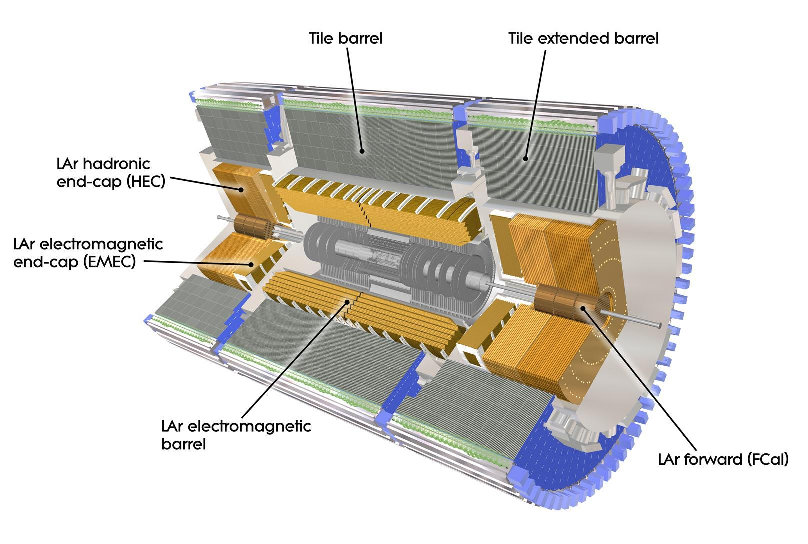
\includegraphics[width=0.9\textwidth]{Fig2/Calorimeters.pdf}
    \caption{Layout of the ATLAS electromagnetic and hadronic calorimeter systems. The total length is $\sim$ 12~m, extending to a maximum radius of 4.25~m.}
    \label{fig:figcalo}
  \end{center}
\end{figure}


\subsubsection{Liquid argon EM calorimeter}
  
The EM calorimeter uses lead as the absorber and liquid Argon as the active material. A photon traversing the absorber will interact with the heavy nucleus via Compton scattering or the photo-electric effect, producing low-energy electrons, or pair production, producing electron/positron pairs. An electron or positron, in turn, can produce bremsstrahlung photons as it is deflected by the nuclei or produce more charged particles via ionization. Thus each incident photon, electron, or positron produces a shower of photons, electrons, and positrons that lose their energy through successive interactions in the absorber. The produced particles ionize the liquid argon, and the charge is collected by electrodes located in the liquid argon gap.  These electrodes consist of three layers of copper sheets, the outer two kept at high-voltage potential and the inner one used to readout the signal.

To provide full coverage in $\phi$ without any cracks, an accordion-shaped absorber and electrode geometry is used, shown in Fig.~\ref{fig:EMacordion}.  This design was chosen to ensure high azimuthal uniformity, a regular liquid argon ionization gap, and a constant sampling fraction within a given detector region. The figure highlights  how this geometry is divided among rectangular cells in $\eta \times \phi$ space, the individual readout elements of varying size,  finely segmented both laterally and longitudinally. Such fine segmentation $– \Delta \eta \times \Delta \phi = 0.025 \times 0.025$ in the second layer of the EM barrel, for example $–$ permits a detailed mapping of the electromagnetic and hadronic showers. 

The position resolution of the EM is driven by the readout geometry (rectangular cells). There are three layers of cells, segmented along the particle's direction of motion.  The $\phi$ segmentation comes from grouping the accordion-shaped electrodes together into a common read out channel. 

In the region $0 <|\eta| < 1.8$ the electromagnetic calorimeters are complemented by a ``presampler'' detector, an instrumented argon layer, which provides a measurement of the energy lost in the solenoid and the outer wall of the barrel cryostat.

The EMEC uses the same accordion geometry as the EMB, whereas the granularity is typically slightly larger than in the barrel.

The signal readout chain for the LAr calorimeter (indeed for all calorimeter systems) is divided into a fast analog readout for the trigger system and a slower digital readout used for more redefined trigger decisions and the offline reconstruction. However, regardless of the readout path, the signal is initiated within the active LAr medium. To minimize noise and increase speed the first level of readout is located on the detector (both for LAr and Tile calorimeter, see~\ref{sec:Tile}). The front-end electronics amplify and shape the signal. Shaping electronics induce a bipolar puse shape in the ionization signal. This shape is characterized by having both a positive and a negative component, which renders the integral of the signal exactly equal to zero.

The performance of the shaping electronics is critical for a correct energy calibration of the detector since the energy is primarily determined from the peak height of the pulse. % Figure??
In each calorimeter region, the overall pulse shape and duration are optimized to approximately cancel a constant injection of energy into the detector. The motivation for this approach is to effectively redefine the baseline of the energy measurement. In the high luminosity environment of the LHC, this reduces the sensitivity to the background from multiple $pp$ interactions on average.

To translate these analog signals to digital signals that can be transmitted long distances to the next stage of the readout system, the pulse shape is measured over several 25~ns (nominal) time intervals, known as samples. The challenge of calorimeter calibration is to map these measured signals to the energy deposited in the active detector medium, known as the visible energy. This calibration is established using test-beam measurements of electrons in the EMB (REFERENCES) and EMEC calorimeters (REFERENCES). 


\begin{figure}[htbp]
  \begin{center}
      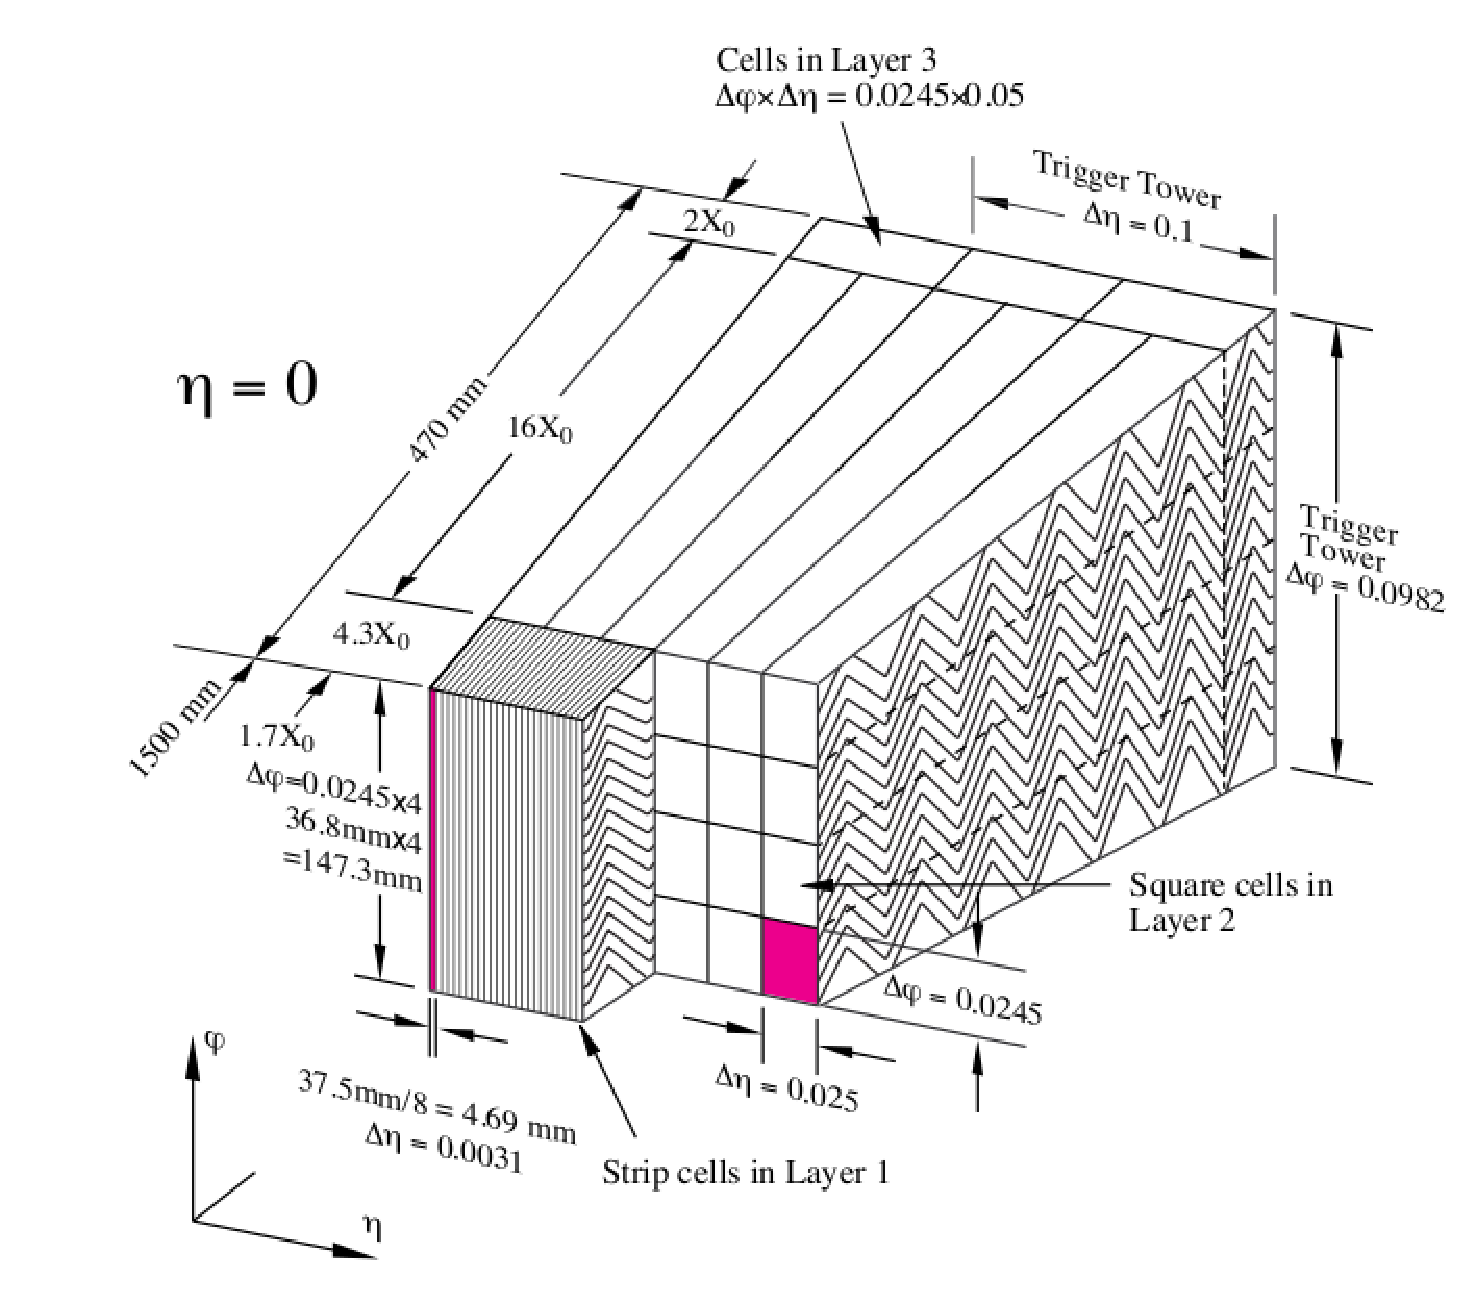
\includegraphics[width=0.9\textwidth]{Fig2/EM_acordionstructure.pdf}
    \caption{Cross section of the LAr barrel calorimeter where the different layers are visible. The granurality in $\eta$ and $\phi$ of the cells of each of the three layers is also shown.}
    \label{fig:EMacordion}
  \end{center}
\end{figure}



\subsubsection{The hadronic calorimeter}\label{sec:Tile}
% TileCal [ ] Tile Calorimeter Technical Design Report, CERN/LHCC 96-42, 15-12-1996;


Outside the EM calorimeter lies the system of hadronic calorimeters. The barrel portion, known as the Tile calorimeter, uses iron absorber slabs interspersed with scintillating tiles. The Tile calorimeter is most notable for its depth of 7.4 radiation lengths ($\lambda$\footnote{To quantify the amount of material needed to capture a particles's energy, the unit of an interaction length, which is the distance over which a high energy charged particle loses $1-\frac{1}{e}\sim 63$\% of its energy , is commonly used.}). The hadronic end-cap and the forward calorimeter, which need to absorb the more energetic particles that are produced at large $|\eta|$, are made of copper and tungsten abosrbers, respectively, with liquid argon as the active material.

The tile calorimeter is composed of 3~mm thick scintillating tiles, arranged to lie parallel  to the incoming particle direction, interleaved with 14~mm thick iron plates. %as shown in Figure!!!!!!!!!!!
It is divided into the barrel calorimeter, covering $|\eta|<1.0$, and two extended barrel calorimeters, covering  $0.8 < |\eta| <1.7$. Each tile is read out by two wavelength-shifting fibers, which convert the scintillator signal to visible light. The readout fibers of several tiles are grouped to a single photomultiplier tube forming cells in $\eta \times \phi$ space. As in the EM calorimeter, these cells are segmented into three layers, the first two of size $\Delta \eta = 0.1$ and  $\Delta \phi = 0.1$ and the last of size   $\Delta \eta = 0.2$ and  $\Delta \phi = 0.1$.  Towers to provide information to the trigger systema are formed from 0.1$\times$0.1 grouping of all three layers.

The HEC uses the LAr active readout design due to the higher radiation tolerance required for the forward regions.  Although housed in the same cryostat as the accordion geometry EMEC, the HEC implements a flat-plate design.

The forward calorimeter extends to cover the region $3.1<|\eta|<4.9$. Since it is the only calorimeter that covers this very forward region, it must provide both electromagnetic and hadronic measurements. In addition, the high particle fluxes in this region necessitate a finely granulated design. The FCal is approximately 10 interaction lenghts deep, and consists of three modules in each end-cap: the first, made of copper, is optimised for electromagnetic measurements, while the other two, made of tungsten, measure predominantly the energy of hadronic interactions.

The hadronic calorimeters are calibrated using muons in test-beam experiments (REFERENCIAS) and those muons produced by cosmic-rays in situ (REFERENCIA). The invariant mass of the $Z$ boson in $Z \rightarrow ee$ events measured in-situ in the 2010 $pp$ collisions is then used to adjust the calibration derived from test-beams and cosmic-muons.





%------------------------------------------------------------------------
\subsection{The Muon System}\label{sec:Muon}
%------------------------------------------------------------------------
 
The muon system gives the ATLAS detector its overall shape and imposing nature, as depicted in Fig.~\ref{fig:MUON1}.
Muons have much smaller cross section to interact in material than electrons and hadrons, for this, they 
do not deposit all their energy in the calorimeters. The muon spectrometer is designed to detect muons within $|\eta|<2.7$. Because many new physics signatures involve high-momentum muons, the system is also required to provide trigger signals based on the particle $\pt$ for  $|\eta|<2.4$.

To provide a momentum measurement, the muons trajectorires are bent in a toroidal magnetic field. This field is provided by one large barrel toroid and two large end-cap toroids, each toroid consisting of eight coils arranged symmetrically around the beam axis.  The toroid system produces a magnetic field that is typically oriented in the $\phi$ direction and that is measured with over 1800 Hall sensors placed throught the magnets. Under the influence of this field, muons are deflected in the $r - z$ plane and the transverse momentum of the muons is given then by the radius of curvature of the tracks. Since the highly-energetic muons bend very little even in this high magnetic field, the muon systema is the largest of all the ATLAS sub-detectors, covering a radius from $\sim$4.5~m to $\sim$12.5~m.

Four  primary subsystems comprise the integrated muon spectrometer: monitored drift tubes (MDT), cathode strip chambers (CSC), resistive plate chambers (RPC) and thing gap chambers (TGC). The MDT and CSC subsytems are primarily designed for precision measurements of muon tracks, width the MDT system providing coverage for the more central region ($|\eta|$ < 2.7, with full coverage only in $|\eta| < 2.0$), whereas the CSC is located in the more forward region ($2.0 < |\eta| < 2.7$) due to its ability to cope with higher background rates. The RPC and TGC muon subsystems are desinged to provide fast, robust readout for use in the trigger and data acquisition system. 

A description of the subsystems can be found elsewhere (REFERENCIAS!!!).
% Describo todos los sub-systems?
%The MDTs utilize a detector technology very similar to the TRT straws, consisting of anode wires running down the centers of cathode tubes filled with Ar/CO_{2} gas. The passage of a charge particle ionizes the gas atoms, creating free charges that drift to the anode. The time difference between signal at the tube and signal at the wire gives the radial distance of the incident muon track to the wire. The tube diameter of $\sim$30~mm and the operating voltage of 3080~V results in a maximum drift time of 700~ns. The position resolution of each drift tube is 80~$\mu$m along the radius of the tube. 



\begin{figure}[htbp]
  \begin{center}
      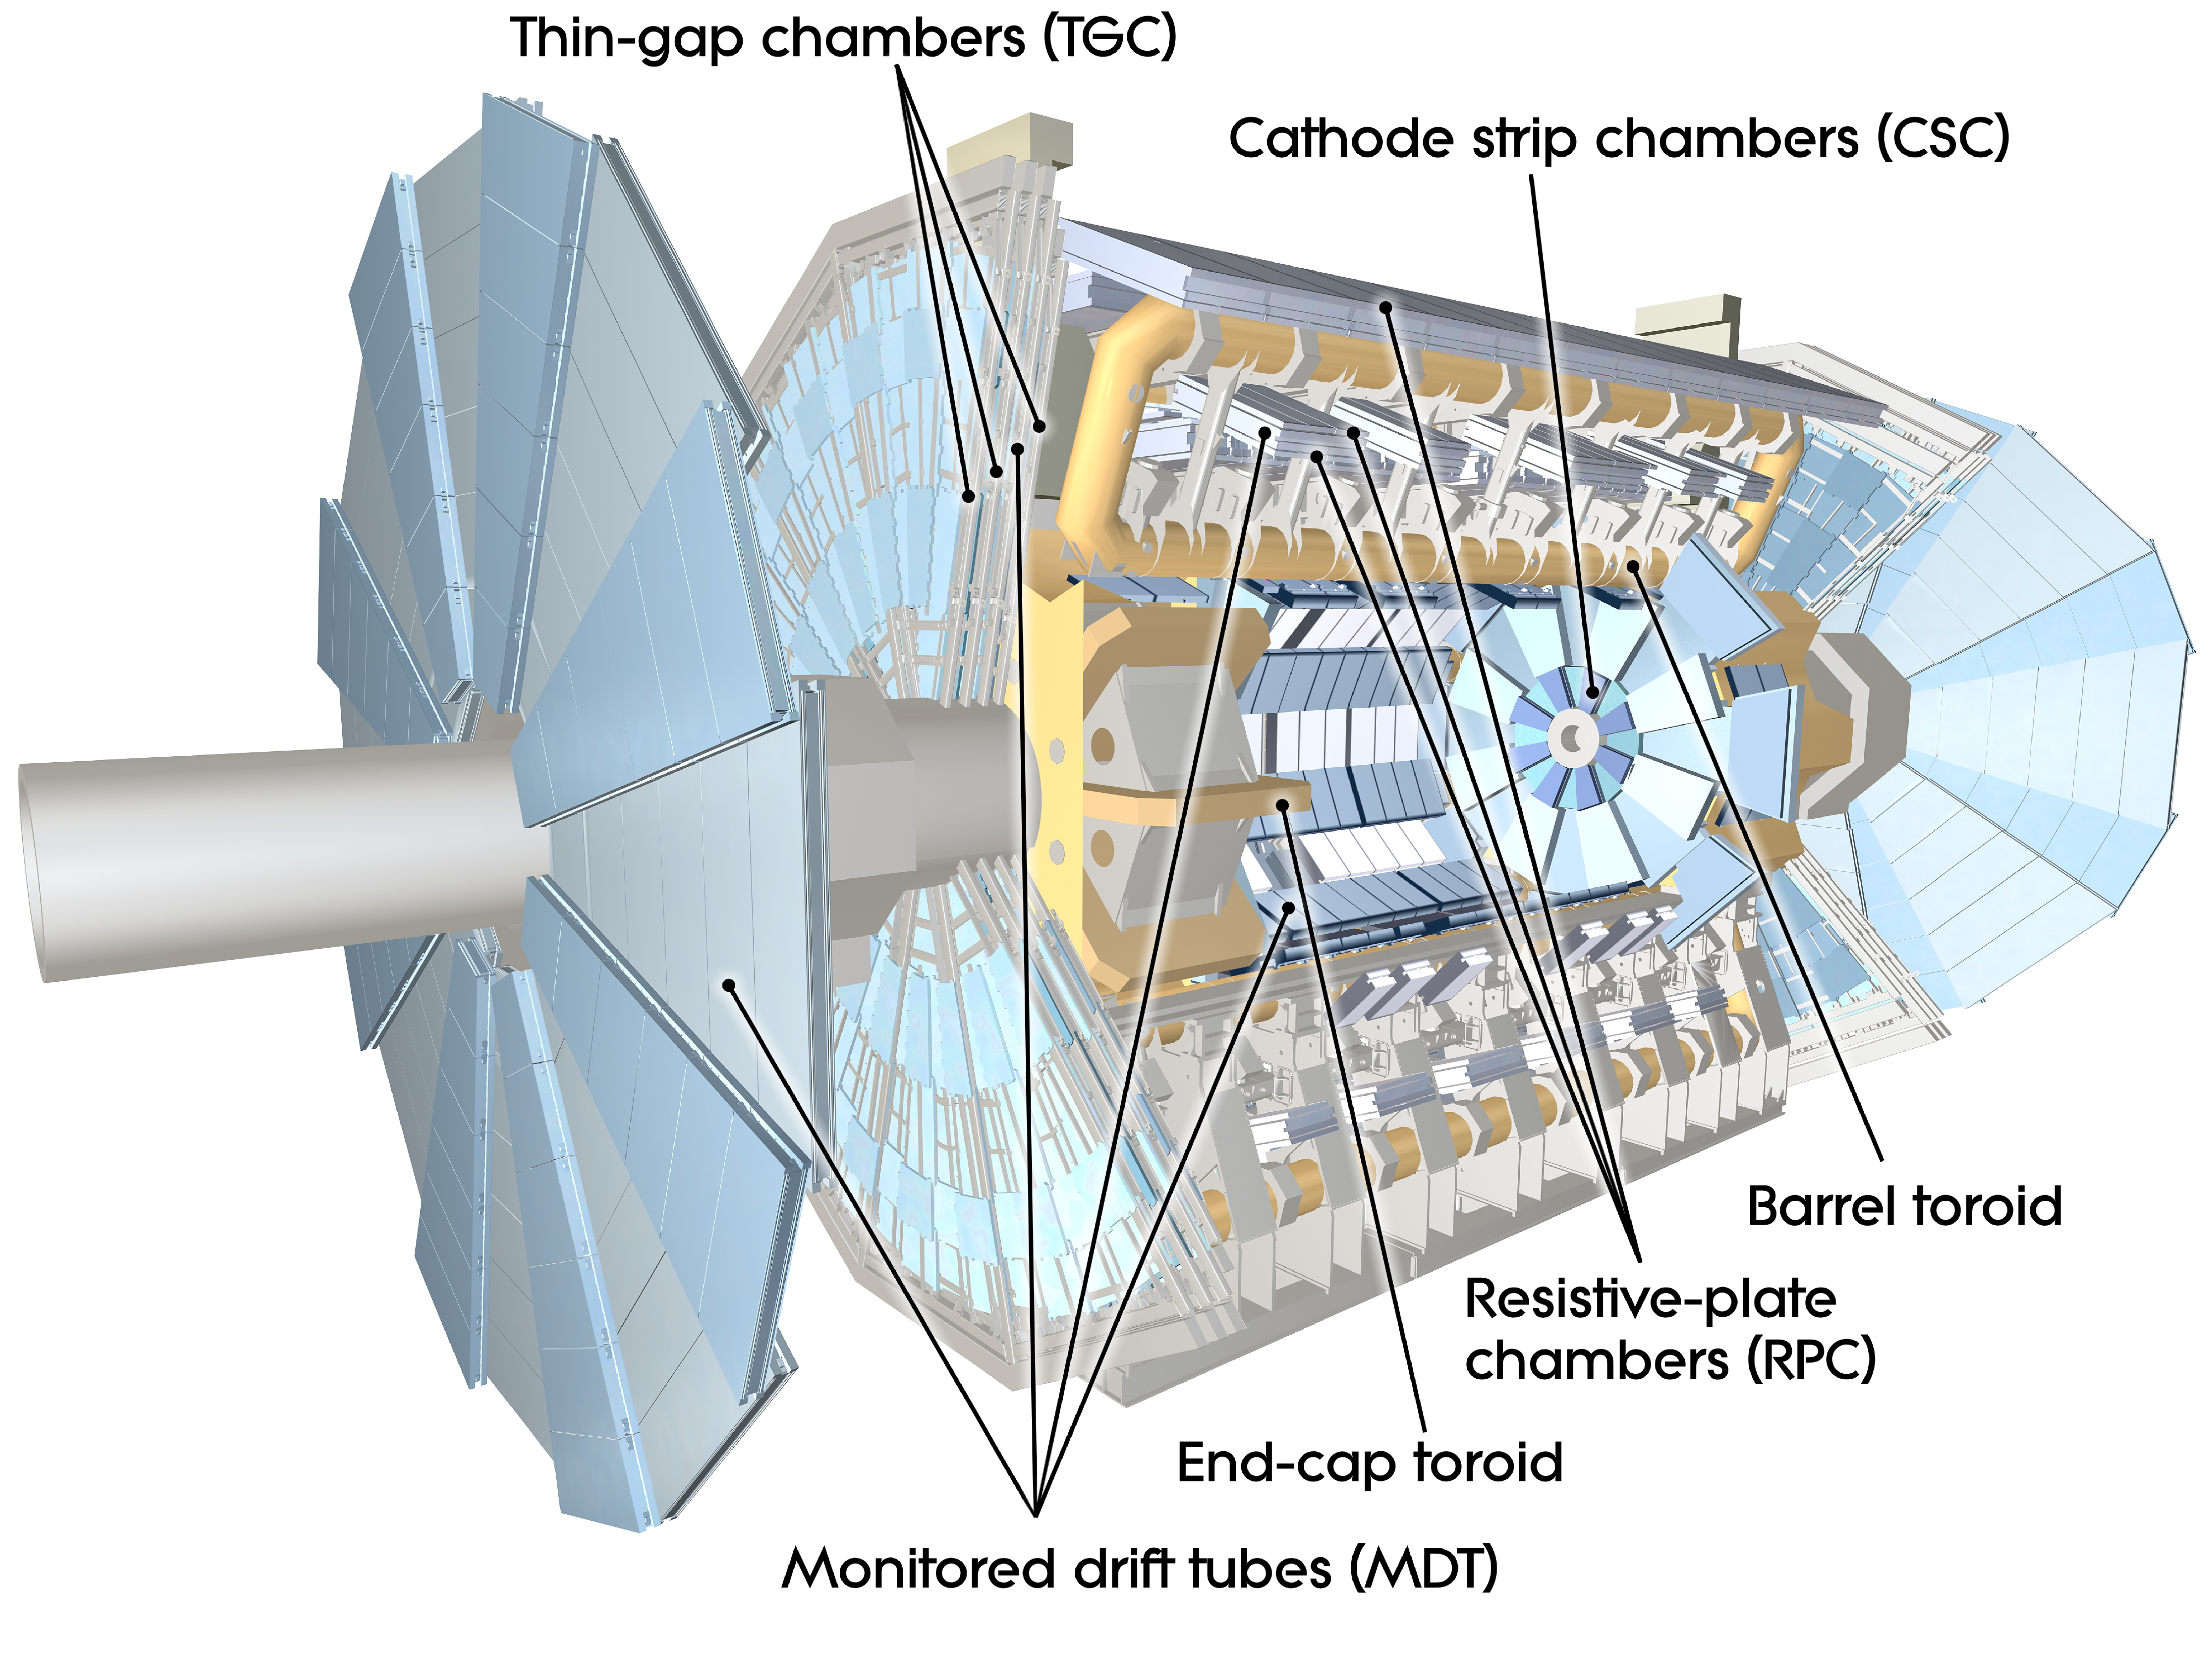
\includegraphics[width=0.8\textwidth]{Fig2/MuonChamber.pdf}
    \caption{Muon Chamber}
    \label{fig:MUON1}
  \end{center}
\end{figure}




%------------------------------------------------------------------------
\subsection{Trigger and Data Adquisition}\label{sec:atlasCALO}
%------------------------------------------------------------------------
 En este cap\'itulo se analiza la estructura del trigger de ATLAS, y el sistema de adquisici\'on y flujo de los datos. Se presenta, asimismo, una breve descripci\'on de los algoritmos usados en la reconstrucci\'on de trayectorias para la selecci\'on de eventos en el detector interno. 


\subsubsection{Arquitectura general}

   El sistema de Trigger y Adquisici\'on de Datos\cite{TDRtdaq} de ATLAS est\'a basado en tres niveles de selecci\'on \emph{online}: Nivel 1, Nivel 2 y Filtro de Eventos. Cada nivel es m\'as lento pero m\'as preciso que el anterior. Trabajando con una frecuencia de interacci\'on de $10^{9}$ Hz y luminosidades del orden de $10^{34}$ $cm^{-2}$ $s^{-1}$, este sistema ser\'a el encargado de reducir la frecuencia de eventos inicial de 40 MHz a 200Hz, que es la velocidad con la que pueden almacenarse. 

   En la figura \ref{fig:TDAQ} se muestra un vista simplificada de los principales componentes y funciones.  

\begin{figure}[!h]
\begin{center}
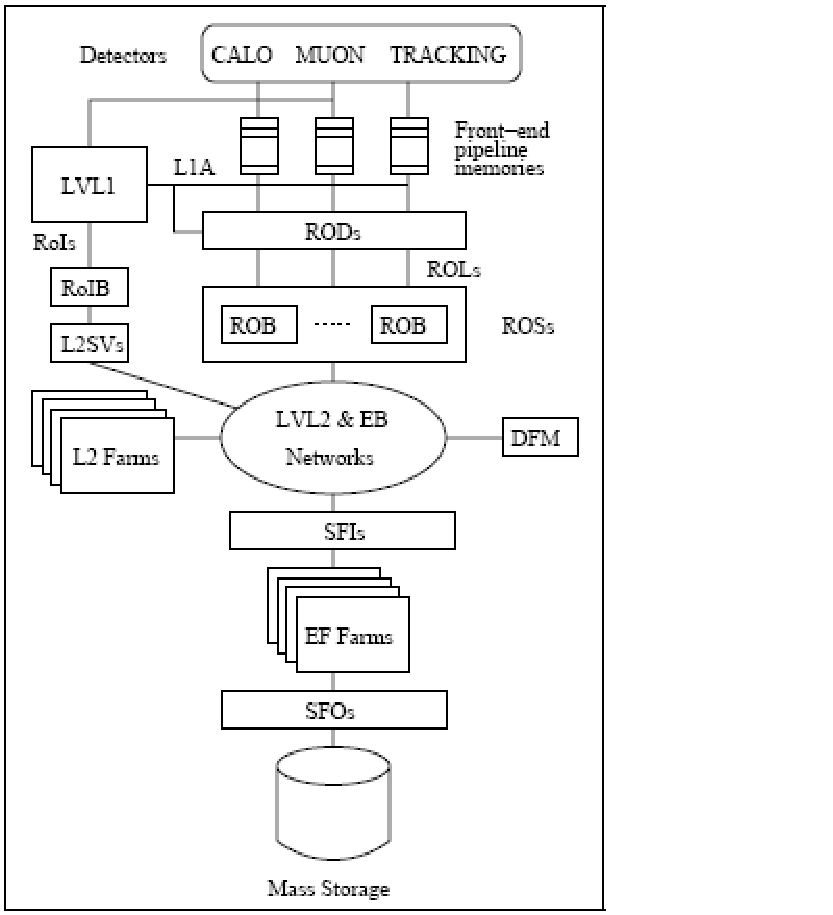
\includegraphics[width=0.5\textwidth]{Fig3/paint_TDAQ.pdf}
\caption{Principales componentes del sistema de trigger y adquisici\'on de datos de ATLAS. } 
\label{fig:TDAQ}
\end{center}
\end{figure}

   El mecanismo que lleva a cabo el movimiento de la informaci\'on (Data Flow System), es el responsable de recibir los datos de los detectores, pasando parte de ellos al sistema de trigger y enviando luego, los eventos seleccionados al lugar de almacenamiento. Siguiendo el esquema de la figura, la comunicaci\'on entre los \emph{drivers} de lectura %controladores de lectura?
de cada detector (RODs) y el sistema de adquisici\'on de datos, est\'a dada por los \emph{buffers} de almacenamiento transitorio (ROBs). La informaci\'on de los eventos aceptados por el Nivel 1 son transportados de los primeros al sistema de lectura (ROS), que consta de numerosos ROBs, guardando los datos a la espera de la decisi\'on del trigger. La informaci\'on requerida por el segundo nivel es provista por estos \'ultimos. Los eventos aceptados son reconstruidos (a partir de fragmentos contenidos en diferentes ROBs) y pasados al siguiente nivel.
%(\emph{Read Out Drivers})
%(\emph{Read Out Buffers})
% (\emph{Read Out System})

   El Nivel 2 y el Filtro de Eventos componen el \emph{High-level Trigger} (HLT) de ATLAS. El Nivel 2 trabaja a la frecuencia de aceptaci\'on del Nivel 1, utilizando una secuencia de r\'apidos algoritmos de selecci\'on que operan t\'ipicamente sobre una fracci\'on de los datos del evento, contenida en regiones del detector previamente seleccionadas por ese nivel (ver el mecanismo de la regi\'on de inter\'es en la siguiente secci\'on). Si la decisi\'on del Nivel 2 es rechazar el evento, los datos del mismo son eliminados de los buffers correspondientes. Si el evento es aceptado,  se reconstruye  en el EB (Event Builder) y es pasado al Filtro de Eventos. Este nivel ejecutar\'a algoritmos de reconstrucci\'on m\'as sofisticados, adaptados de aquellos para el an\'alisis \emph{offline}, utilizando informaci\'on detallada de los detectores para efectuar el proceso de selecci\'on final, que determinar\'a cu\'ales son los eventos que ser\'an guardados para posteriores estudios.

  En las siguientes secciones se presenta una descripci\'on m\'as detallada de los niveles de trigger.

 
\subsubsection{El Nivel 1}

   El primer nivel de trigger de ATLAS es implementado mediante hardware. \'Este realiza una decisi\'on inicial a partir de la informaci\'on provista por los calor\'imetros y del detector de muones, basando su estrategia en la combinaci\'on de objetos en coincidencia. %or veto.
  
   En el sistema de muones, los candidatos de alto momento transverso son identificados en las c\'amaras especiales de trigger: RPCs en el barril y TGCs en las tapas. En el caso del calor\'imetro, se definen una serie de conjuntos de umbrales de $p_T$ para cada objeto (electrones, fotones, jets, etc.), seleccionando aquellos que pasen los criterios de selecci\'on correspondientes al evento f\'isico de inter\'es. 

   Puesto que la decisi\'on de aceptar un evento no puede ser realizada en los 25 ns que median entre dos cruces de \emph{bunches}, los subdetectores almacenan localmente la informaci\'on del mismo en \emph{pipelined buffers} hasta que el Nivel 1 efect\'ua la selecci\'on. Luego, los datos son enviados a los RODs especi\'ficos de cada detector para luego dirigirse a los ROBs, donde son almacenados hasta que la decisi\'on del Nivel 2 sea alcanzada. 
   Cuando un evento es aceptado, el Nivel 1 comunica la decisi\'on al mecanismo que se encargar\'a de construir una Regi\'on de Inter\'es (RoI). Este mecanismo es una importante pieza sobre la que descansa la estrategia del sistema de trigger; a trav\'es del mismo, el Nivel 2 har\'a uso de la informaci\'on del evento en regiones localizadas del detector, de manera que los algoritmos de reconstrucci\'on en ese nivel s\'olo transfieran los ROBs necesarios para arribar a una r\'apida decisi\'on. %Es importante notar que la informaci\'on de todos los subdetectores est\'a disponible para dichos algoritmos en caso de ser necesario.
La RoI contendr\'a la informaci\'on de la posici\'on ($\eta$ y $\phi$) y el momento de los objetos candidatos.

   Este nivel est\'a dise\~nado para llevar a cabo su decisi\'on en un tiempo menor a 2.5 $\mu$s, medidos desde la colisi\'on \emph{p-p}, hasta que la informaci\'on del evento est\'a disponible en la electr\'onica de salida de los detectores. En este proceso la frecuencia de eventos ser\'a reducida a 75KHz (l\'imite fijado por la electr\'onica).

\subsection{El HLT}

 El High-level Trigger de ATLAS abarca la segunda y tercera etapa de la selecci\'on de eventos. Comprende el Nivel 2 y el Filtro de Eventos, y contiene adem\'as, el Software de Selecci\'on (ESS). Este \'ultimo comparte la estructura usada por el Offline para los c\'odigos de selecci\'on, facilitando el an\'alisis \emph{offline} de los datos, y el desarrollo de algoritmos en el HLT.

   El punto de entrada del trigger es el resultado del Nivel 1. \'Este provee informaci\'on acerca de la regi\'on de inter\'es, fundamental para el r\'apido funcionamiento de los algoritmos del Nivel 2. As\'i, los datos del Nivel 1 gu\'ian la selecci\'on del Nivel 2; y \'esta a su vez guiar\'a la del Filtro de eventos, como se ilustra en la figura \ref{fig:HLTchainseed}. 
%HLTchain_seeding.pdf
\begin{figure}[!h]
\begin{center}
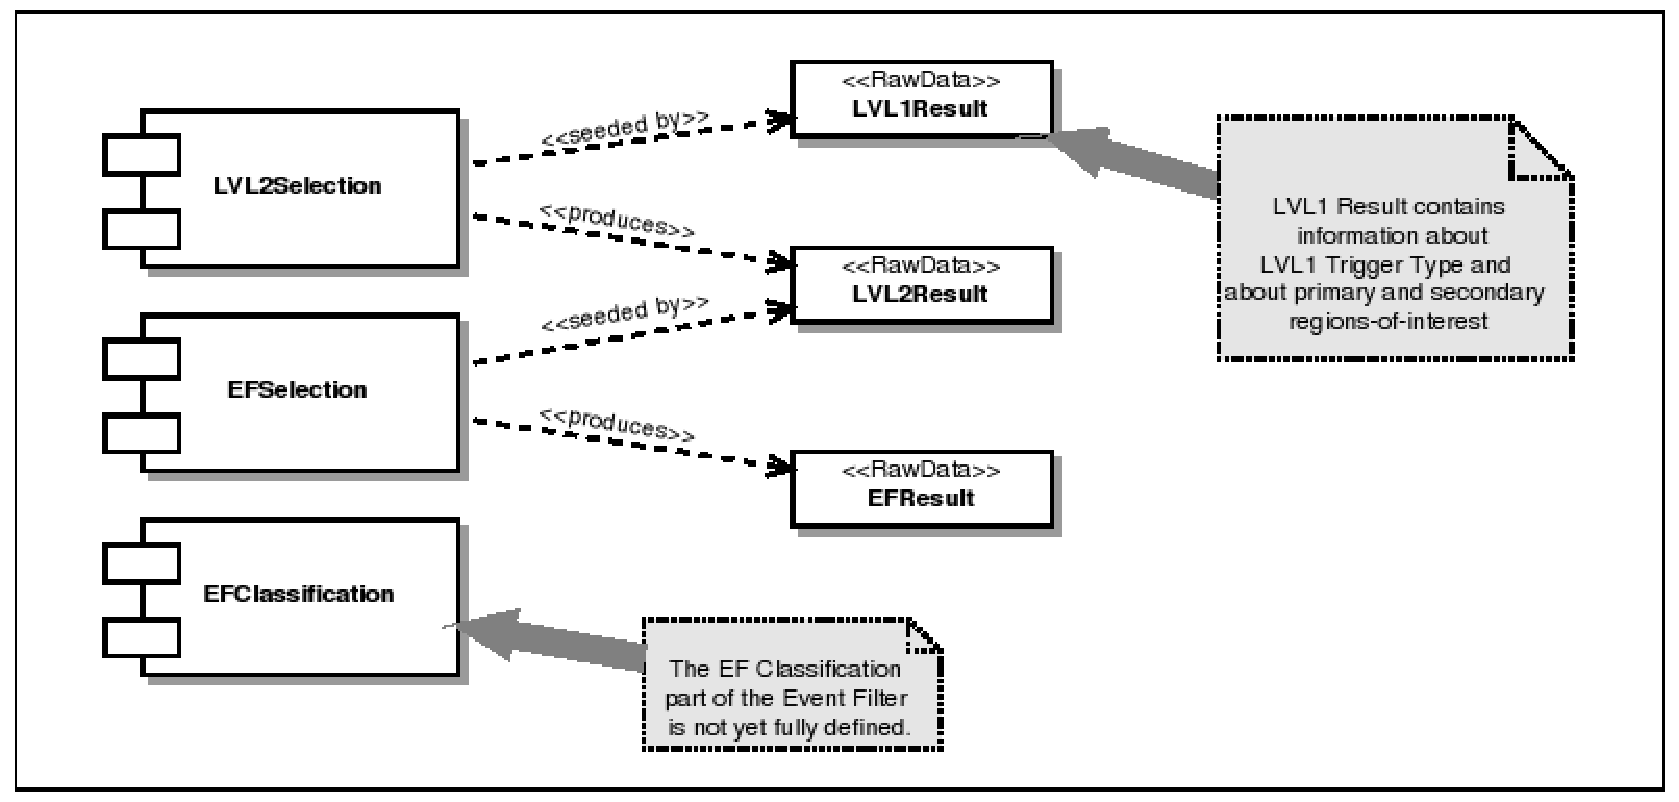
\includegraphics[width=0.9\textwidth]{Fig3/HLTchain_seeding.pdf} 
\caption{Cadena de selecci\'on del \emph{High-level Trigger} de ATLAS. Cada nivel es guiado por el resultado del paso anterior.}
\label{fig:HLTchainseed}
\end{center}
\end{figure}


\subsubsection{El Nivel 2}
   La tarea espec\'ifica del Nivel 2 es reducir la frecuencia de eventos de $\sim$ 100 kHz a alrededor de 2 kHz, combinando la informaci\'on de todos los detectores para su decisi\'on global. A diferencia del Nivel 1, esta segunda etapa de selecci\'on realiza operaciones no sincronizadas sobre los eventos, con un tiempo de decisi\'on de 10 ms.
%asynchronous??

   El Nivel 2 utiliza las regiones de inter\'es provistas por el Nivel 1. Cada regi\'on es examinada en el subdetector de origen (calor\'imetro o sistema de muones) para su confirmaci\'on; para luego buscar informaci\'on de otros subdetectores. En el caso del trigger de muones, el poder de rechazo del Nivel 2 proviene de ajustar los umbrales de $p_{T}$, respecto de los utilizados en el primer nivel, a partir de la informaci\'on de las c\'amaras de precisi\'on del sistema de muones (MDTs) y la correspondiente al detector interno.
Los procesadores del Nivel 2 son los encargados de ejecutar luego el software de selecci\'on de eventos, utilizando la informaci\'on almacenada en los \emph{buffers}. Usando las RoIs del Nivel 1, el Nivel 2 acceder\'a de manera selectiva a los datos en los ROBs, moviendo s\'olo la informaci\'on requerida para efectuar la decisi\'on. T\'ipicamente, s\'olo una peque\~na fracci\'on del detector, correspondiente a las regiones centradas en los objetos indicados por el Nivel 1, ser\'an necesitados por el segundo nivel.

  Hasta que un evento es aceptado o rechazado (en $\sim$ 10 ms), los datos son retenidos en los ROBs. En caso de aceptaci\'on, los fragmentos del evento almacenados en distintos buffers ser\'an requeridos por el sistema de control del Nivel 2 (L2SVs) para ser enviados al constructor de eventos (EB). El evento ensamblado es guardado en una \'unica direcci\'on de memoria para ser utilizado por el Filtro de Eventos. El tama\~no promedio de un evento ser\'a del orden de 1,5 MB.


\subsubsection{El Filtro de Eventos}

  Luego del Nivel 2, la \'ultima etapa de selecci\'on \emph{online} es realizada por el Filtro de Eventos (EF). El EF emplea algoritmos y m\'etodos similares a los implementados en el an\'alisis \emph{offline}, adaptados para su corrida en el tiempo real del experimento; su poder de rechazo radica en el uso de algoritmos y criterios de selecci\'on m\'as complejos, que por l\'imites en el tiempo de procesamiento no pueden ser utilizados en el Nivel 2.
  
  El EF utilizar\'a informaci\'on actualizada de la calibraci\'on y alineamiento del detector y un completo mapa del campo magn\'etico; llevando a cabo con ello la selecci\'on final del evento f\'isico que ser\'a guardado para su estudio en el Offline. La frecuencia de aceptaci\'on del nivel anterior ser\'a reducida en un orden de magnitud, almacenando a una tasa de $\sim$100 MB/s.


\subsubsection{El software de selecci\'on}
\label{'HLTalgos'}
   
 La tarea del software de selecci\'on (ESS) es la selecci\'on y clasificaci\'on de los eventos. Candidatos tales como electrones, jets, muones, etc., representados por objetos abstractos, son reconstruidos utilizando un particular conjunto de algoritmos. Un evento es seleccionado si el objeto reconstruido satisface al menos una de las signaturas establecidas en el men\'u del sistema de disparo. En el Nivel 2 y el Filtro de Eventos (EF), los eventos ser\'an rechazados si no pasan los espec\'ificos criterios de selecci\'on, dise\~nados para la reducci\'on de la frecuencia de eventos, al l\'imite dado por la velocidad a la que \'estos pueden ser almacenados.

 El ESS se compone de una infraestructura y un conjunto de programas de selecci\'on para las dos etapas del HLT.  Los algoritmos de reconstrucci\'on para el trigger est\'an basados en aquellos utilizados para la reconstrucci\'on \emph{offline}, pero correr\'an \emph{online} en el entorno de software provisto por los procesadores del Nivel 2 y el EF. 

  De manera de facilitar el desarrollo de los algoritmos del HLT y simplificar los estudios del Offline; el ESS ha sido dise\~nado de manera de poder ser ejecutado directamente en el entorno provisto por la estructura de software de an\'alisis offline del experimento, ATHENA\cite{Athena}. La estructura dada por este paquete de software es lo suficientemente flexible como para abarcar una variedad de procesos, incluyendo no s\'olo algoritmos de trigger sino tambi\'en tareas de calibraci\'on y monitoreo. Se ha destinado un ap\'endice (A) para su descripci\'on.
 
  En el Offline, la tarea del ESS es la de emular la cadena completa de selecci\'on \emph{online}. Para su ejecuci\'on el sistema se sirve de cuatro sub-paquetes: el direccionamiento o \emph{Steering}, los algoritmos del HLT, y los paquetes de software para la clasificaci\'on y movimiento de los datos, EDM (\emph{Event Data Model}) y el DM (\emph{Data Manager}). Los \'ultimos toman los datos del evento en el formato que poseen a la salida de los sistemas de lectura (\emph{Raw data} en formato \emph{byte stream}), y los convierten en objetos que puedan ser usados por los algoritmos en la cadena de selecci\'on (\emph{Raw Data Objects}).

  La tarea de los algoritmos del HLT es la de analizar los datos del evento, reconstruyendo partes del mismo, luego de la selecci\'on del Nivel 1. El paquete se compone de dos subconjuntos principales:
%itemize
\begin{itemize}
   \item Programas de preparaci\'on de datos. Son los algoritmos ejecutados por los sistemas EDM y DM para la conversi\'on del formato de los datos del evento. 
   \item Algoritmos FEX o de \emph{Feature Extraction}. Comprende los programas de reconstrucci\'on y los llamados algoritmos de ``hip\'otesis''. Estos \'ultimos (a los primeros nos referiremos en la siguiente secci\'on) son aquellos programas que se encargan de eliminar, una vez realizada la reconstrucci\'on, aquellos candidatos que no cumplen con las caracter\'isticas o atributos asignados al evento f\'isico en consideraci\'on (hip\'otesis), aplicando espec\'ificos criterios de selecci\'on. La presencia de los algoritmos de hip\'otesis es fundamental en la secuencia del HLT ya que evita la ejecuci\'on innecesaria de algoritmos al descartar eventos en las primeras etapas de la cadena.
\end{itemize}

  Por \'ultimo, el subpaquete de \emph{Steering} es aquel que organiza el procesamiento de los datos del evento en el Nivel 2 y el Filtro de eventos; controlando el orden en el que los algoritmos de reconstrucci\'on e hip\'otesis son ejecutados. El Steering define la secuencia del HLT, y manipula los resultados en cada paso de selecci\'on de manera que la decisi\'on del trigger sea alcanzada.


%------------------------------------------------------------------------
\subsection{Data quality}\label{sec:atlasSim}
%------------------------------------------------------------------------

%------------------------------------------------------------------------
\subsection{Simulation of particle interactions in the ATLAS Detector}\label{sec:atlasSim}
%------------------------------------------------------------------------



 
%%
%%%%%%%%%%%%%%%%%%%%%%%%%%%%%%%%%%%%%%%%%%%%%%%%%%%%%%%%%%%%%%%%%%%%%%%%%%%%%%%
% Object reconstruction and event selection
%%%%%%%%%%%%%%%%%%%%%%%%%%%%%%%%%%%%%%%%%%%%%%%%%%%%%%%%%%%%%%%%%%%%%%%%%%%%%%%
%

\chapter{Event reconstruction and \emph{\textbf{b}}-Tagging }\label{ch:reco}


The event reconstruction software, which in ATLAS is implemented in the software framework {\sc athena}~\cite{Calafiura2005zz}, process the events starting from the raw data obtained from the various sub-detectors (energy deposits and hits), processing them in many different stages and finally interpreting them as a set of charged tracks, electrons, photons, jets, muons and, in general, of possible kinds of final state objects with related four momenta.  
In this chapter the reconstruction of these objects is briefly described together with the algorithms for the identification of $b$-quark jets.  These algorithms are mainly based on the reconstruction of the primary interaction vertex, on the reconstruction of charged particles in the Inner Detector and on the reconstruction of jets in the calorimeter.   

%------------------------------------------------------------------------
\section{Jet reconstruction and calibration}\label{sec:ObjSelection}
%------------------------------------------------------------------------

Hadronic jets used for ATLAS analyses are reconstructed by a jet algorithm, starting from the energy depositions of electromagnetic and hadronic showers in the calorimeters.  Two different size parameters are used: $R = 0.4$, for narrow jets, and $R = 0.6$, for wider jets. The default jet algorithm is the anti-$k_t$ algorithm, described in Chapter~\ref{ch:theory}. Due to the expected level of pile-up in the LHC, the primary factor that influenced the selection of this algorithm was the effect of multiple simultaneous interactions on the reconstruction of jets. The original ATLAS cone algorithm, known to contain infrared and collinear sensitivity, is highly susceptible to this effect. On the contrary, the anti-$k_t$ algorithm is the most stable after the introduction of pile-up~\cite{Asquith:1311867}.  

The input to calorimeter jet reconstruction can be calorimeter towers or topological cell clusters. Charged particle tracks reconstructed in the Inner Detectors are also used to define jets. The latter have the further advantage of being insensitive to pile-up and they provide a stable reference for systematic studies. The jet inputs are combined as massless four-momentum objects in order to form the final four-momentum of the jet, which allows for a well-defined jet mass~\cite{Busato:1271710}. In the case of track-jets, the track four-momentum is constructed assuming the $\pi$ meson mass for each track.

Calorimeter towers are static, $\Delta \eta \times \Delta \phi = 0.1 \times 0.1$, grid elements built directly from calorimeter cells. There are two types of calorimeter towers: with or without noise supression. The latter are called ``noise-suppressed'' towers and use only the cells with energies above a certain noise threshold.  The noise of a calorimeter cell is measured by recording calorimeter signals in periods where no beam is present in the acelerator.  The standard deviation $\sigma$ around the mean measured energy is interpreted as the noise of the cell, and dependes on the sampling layer in which the cell resides and the position in $\eta$.

The results presented in this thesis show jets which were built from noise-suppressed topological clusters of energy in the calorimeter, aslo known as ``topo-clusters''~\cite{topoClusters}. Topological clusters are groups of calorimeter cells that are designed to follow the shower development taking advantage of the fine segmentation of the ATLAS calorimeters. The topological cluster formation starts from a seed cell with $|E_{cell}| > 4 \sigma$ above the noise. In a second step, neighbor cells that have an energy at least 2$\sigma$ above their mean noise are added to the cluster. Finally, all nearest-neighbor cells surrounding the clustered cells are added to the cluster, regardless of signal-to-noise ratio\footnote{Noise-supressed towers also make use of the topological clusters algorithm~\cite{topoClusters} to select cells, i.e. only calorimeter cells that are included in topo-clusters are used.}. The position of the cluster is assigned as the energy-weighted centroid of all constituent cells (the weight used is the absolute cell energy).

In Monte Carlo simulation, reference jets (``truth jets'') are formed from simulated stable particles using the jet algorithm utilized for the reconstructed jets. 

\subsubsection{Jet calibration}\label{sec:calib}

The purpose of the jet energy calibration, or jet energy scale (JES), is to correct the measured electromagnetic scale (EM scale) energy to the energy of the stable particles within a jet.  The jet energy calibration must account then for the calorimeter non-compensation; the energy lost in inactive regions of the detector, such as in the cryostat walls or cabling; energy that escapes the calorimeters, such as that of highly-energetic particles that ``punch-through'' to the muon system; energy of cells that are not included in clusters, due to inefficiencies in the noise-suppression scheme; and energy of clusters not included in the final reconstructed jet, due to inefficiencies in the jet reconstruction algorithm. The muons and neutrinos that may be present within the jet are not expected to interact within the calorimeters, and are not included in this energy calibration.
Due to the varying calorimeter coverage, detector technology, and amount of upstream inactive material, the calibration that must be applied to each jet to bring it to the hadronic scale varies with its $\eta$ position within the detector. 

The jet energy is first reconstructed from the constituent cell energies at EM scale. These cells have been calibrated to return the energy corresponding to electromagnetic showers in the calorimeter, based on test-beam injection of electrons and pions~\cite{Aharrouche2006601},  measurements of cosmic muons~\cite{Cooke:1071187} and the reconstruction of the $Z$ mass peak in $Z \rightarrow ee$ decays~\cite{Aad:2011mk}. The correction for the lower response to hadrons is based on the topology of the energy depositions observed in the calorimeter. 

In the simplest case the measured jet energy is corrected, on average, using Monte Carlo simulations, as follows:
%
\begin{equation}
E^{jet}_{calib} = E^{jet}_{meas} /F_{calib}(E^{jet}_{meas}),\; \; \mbox{with} \;  E^{jet}_{meas} = E^{jet}_{EM} - O(\mbox{NPV}),
\end{equation}
%
where $E^{jet}_{EM}$ is the calorimeter energy measured at the electromagnetic scale, $E^{jet}_{calib}$ is the calibrated energy and $\emph{F}_{calib}$ is the calibration function that depends on the measured jet energy and is evaluated in small jet $\eta$ regions. The variable $ O(\mbox{NPV})$ denotes the correction for additional energy from multiple proton-proton interactions depending on the number of primary vertices (NPV).

The simplest calibration scheme and the one used in this thesis is the so called ``EM+JES''. This calibration applies the corrections as a function of the jet energy and pseudorapidity to jets reconstructed at the electromagnetic scale.  The additional energy due to multiple proton-proton collisions within the same bunch crossing (pile-up) is corrected before the hadronic energy scale is restored, such that the derivation of the jet energy scale calibration is factorised and does not depend on the number of additional interactions in the event. The EM+JES calibration scheme consists of three subsequent steps:

\begin{itemize}
\item
Pile-up correction: An offset correction is applied in order to substract the additional average energy measured in the calorimeter due to multiple proton-proton interactions. This correction is derived from minimum bias data as a function of NPV, the jet pseudorapidity and the bunch spacing.
\item
Vertex correction: The jet four momentum is corrected such that the jet originates from the primary vertex of the interaction instead of the geometrical centre of the detector. 
\item
Jet energy and direction correction: The jet energy and direction are corrected using constants derived from the comparison of the kinematic observables of reconstructed jets and those from truth jets in the simulation.
\end{itemize}

In the final step the calibration is derived in terms of the energy response of the jet, or the ratio of the reconstructed jet energy to that of a truth jet.  The EM scale response is written as,
%
\begin{equation}
R^{jet}_{EM} = E^{jet}_{EM} / E^{jet}_{truth}
\end{equation}
%
To compute this quantity, reconstructed jets must be matched to isolated jets in the Monte Carlo within $\Delta R < 0.3$. The isolation requirement is applied in order to factorize the effects due to close-by jets from those due to purely detector effects such as dead material and non-compensation. The isolation criterion requires that no other jet with a $\pt > 7$~GeV be within $\Delta R < 2.5R$, where $R$ is the distance parameter of the jet algorithm. The EM scale energy response is binned in truth jet energy, $E^{jet}_{truth}$, and the calorimeter jet detector $\eta$.  For each $(E^{jet}_{truth}, \eta)$-bin, the averaged jet response is defined as the peak position of a Gaussian fit to the $E^{jet}_{EM} / E^{jet}_{truth}$ distribution.  A function $F_{calib,k}(E^{jet}_{EM})$ is then defined for each $\eta$-bin $k$ that describes the response as a function of the uncalibrated jet energy. $F_{calib,k}(E^{jet}_{EM})$ is parameterised as:
%
\begin{equation}
F_{calib,k}(E^{jet}_{EM}) = \sum_{i=0}^{N_{max}} a_i (\ln E^{jet}_{EM})^i,
\end{equation}
%
where $a_i$ are free parameters, and $N_{max}$ is chosen between 1 and 6 depending on the goodness of the fit. The final jet energy scale correction that relates the measured calorimeter jet energy scale to the hadronic scale is then defined as $1/F_{calib,k}(E^{jet}_{EM})$ in the following:
%
\begin{equation}
E^{jet}_{EM+JES} = \frac{E^{jet}_{EM}}{F_{calib}(E^{jet}_{EM})|_{\eta}},
\end{equation}
%
where $F_{calib}(E^{jet}_{EM})|_{\eta}$  is $F_{calib,k}(E^{jet}_{EM})$ for the relevant $\eta$-bin $k$.


Other calibrations schemes are the global calorimeter cell weighting (GCW) calibration and the local cluster weighting (LCW) calibration.  The GCW scheme exploits the observation that electromagnetic showers in the calorimeter leave more compact energy depositions than hadronic showers with the same energy.  Energy corrections are derived for each cell within a jet.  The cell corrections account for all energy loses of a jet in the detector. Since these corrections are only applicable to jets and not to energy depositions, they are called ``global'' corrections.

The LCW calibration method first classifies topo-clusters as either electromagnetic of hadronic, based on the measured energy density. Energy corrections are derived according to this classification from single charged and neutral pion Monte Carlo simulations. Dedicated corrections are derived for the effects of non-compensation, signal losses due to noise threshold effects, and energy lost in non-instrumented regions. Since the energy corrections are applied without reference to a jet definition they are called ``local'' corrections. Jets are then built from these calibrated clusters using a jet algorithm.  

The final jet energy calibration can be applied to EM scale jets, with the resulting calibrated jets referred to as EM+JES, or to LCW (GCW) calibrated jets, with the resulting jets referred to as LCW+JES (GCW+JES) jets.

A further jet calibration scheme called global sequential (GS) calibration, starts from jets calibrated with the EM+JES calibration and exploits the topology of the energy deposits in the calorimeter to characterise fluctuations in the jet particle content of the hadronic shower development.  Correcting for such fluctuations can improve the jet energy resolution. The correction uses several jet properties, and each correction is applied sequentially.


For the 2011 data the recomended calibration schemes were the EM+JES and the LCW calibrations. The simple EM+JES calibration does not provide the best performance, but allows in the central detector region the most direct evaluation of the systematic uncertainties from the calorimeter response to single isolated hadrons measured \emph{in situ}  and in test-beams and from systematic variations in the Monte Carlo simulation.  For the LCW+JES calibration scheme the JES uncertainty is determined from \emph{in situ}  techniques. For all calibration schemes, the JES uncertainty in the forward regions is derived from the uncertainty in the central region using the transverse momentum balance in events where only two jets are produced. 



\subsubsection{Jet energy scale uncertainties for the EM+JES scheme}

For many physics analyses, the uncertainty on the JES constitutes the dominant systematic uncertainty because of its tendency to shift jets in and out of analysis selections due to the steeply falling jet $\pt$ spectrum. The uncertainty on the EM+JES scale  is determined primarily by six factors:  varying the physics models for hadronization and parameters of the Monte Carlo generators, evaluating the baseline calorimeter response to single particles, comparing multiple models for the detector simulation of hadronic showers, assesing the calibration scales as a function of pseudorapidity, and by adjusting the JES calibration methods itself.  The final JES uncertainty in the central region, $|\eta| < 0.8$, is determined from the maximum deviation in response observed with respect to the response in the nominal sample.  For the more forward region, the so called ``$\eta$-intercalibration'' contribution is estimated. This is a procedure that uses direct di-jet balance measurements in two-jet events to measure the relative energy scale of jets in the more forward regions compared to jets in a reference region. The technique exploits the fact that these jets are expected to have equal $\pt$ due to transverse momentum conservation. Figure~\ref{fig:JESuncertainty}  shows the final fractional jet energy scale uncertainty and its individual contributions as a function of $\pt$ for a central $\eta$ region. The JES uncertainty for anti-$k_t$ jets with $R = 0.4$ is between $\approx$4\% (8\%, 14\%) at low jet $\pt$ and $\approx$2.5\%-3\% (2.5\%-3.5\%, 5\%) for jets with $\pt > 60$~GeV in the central (endcap, forward) region.

\begin{figure}[htbp]
  \begin{center}
   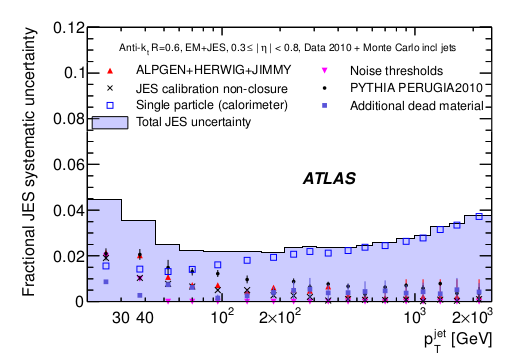
\includegraphics[width=0.9\textwidth]{JESUncertainty.png}
    \caption{Fractional jet energy scale uncertainty as a function of jet $\pt$ for jets in the pseudorapidity region 0.3$ < |\eta| < $0.8 in the calorimeter barrel. The total uncertainty is shown as the solid tight blue area. The individual sources are also shown.}
    \label{fig:JESuncertainty}
  \end{center}
\end{figure}

In addition to the tests above, \emph{in situ} tests of the JES using direct $\gamma$-jet balance, multi-jet balance, and track-jets indicate that the uncertainties in Fig.~\ref{fig:JESuncertainty} reflect accurately the true uncertainties in the JES.  

In the case of jets induced by bottom quarks ($b$-jets), the calorimeter response uncertainties are also evaluated using single hadron response measurements \emph{in situ}  and in test beams~\cite{ATLAS-CONF-2011-028}. For jets within $|\eta|<0.8$ and $20 \leq \pt < 250$~GeV the expected difference in the calorimeter response uncertainty of identified $b$-jets with respect to the one of inclusive jets is less than 0.5\%. It is assumed that this uncertainty extends up to $|\eta| < 2.5$.
% Single hadrons with momenta up to 20GeV are selected in minimum bias sample produced in pp collisions at 7TeV taken in 2011 and the calorimeter energy (E) in a narrow cone around an isolated track is compared to the track momentum (p). In this method, jets are treated as a superposition of energy deposits of single particles. For each calorimeter deposition within the jet cone, the type of the particle inside the jet is determined and the expected mean shift and the systematic uncertainty of the calorimeter response between data and monte carlo simulation is evaluated.

The JES uncertainty arising from the modelling of the $b$-quark fragmentation can be determined from systematics variations of the Monte Carlo simulation. The fragmentation function is used to estimate the momentum carried by the $b$-hadron with respect to that of the $b$-quark after quark fragmentation.   The fragmentation function included in {\sc pythia} originates from a detailed study of the $b$-quark fragmentation function in comparison with OPAL~\cite{Abbiendi:2002vt} and SLD~\cite{Abe:2002iq} data. To assess the impact of the $b$-fragmentation, the nominal parameters of the {\sc pythia} fragmentation function are replaced by the values from a tune using the Professor framework~\cite{Professor}. In addition, the nominal fragmentation function is replaced by the modified Bowler-Lund fragmentation function~\cite{BowlerLund}. The $b$-jet response uncertainty is evaluated from the ratio between the response of $b$-jets in the varied Monte Carlo samples to the nominal {\sc pythia}. The response variations are well within 2\%.

The $b$-jet JES uncertainty is obtained adding the calorimeter response uncertainty and the uncertainties from the systematic Monte Carlo variations in quadrature. The resulting additional JES uncertainty for $b$-jets is shown in Fig.~\ref{fig:bjetJESuncertainty}. It is about 2\% up to $\pt \approx 100$~GeV and below 1\% for higher $\pt$. To obtain the overall $b$-jet uncertainty this uncertainty is added in quadrature to the JES uncertainty for inclusive jets.

\begin{figure}[htbp]
  \begin{center}
      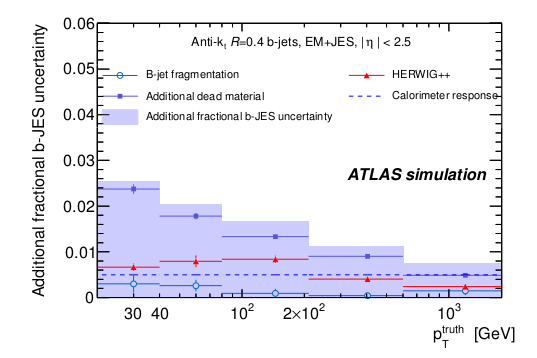
\includegraphics[width=0.9\textwidth]{bjetsJESUncertainty.png}
    \caption{Additional fractional $b$-jet JES uncertainty as a function of the truth jet transverse momentum for anti-$k_t$ jets with $R=0.4$ calibrated with EM+JES scheme for $|\eta| < 2.5$. Shown are systematic Monte Carlo variations using different modelling of the $b$-quark fragmentation and physics effects as well as variations in the detector geometry and the uncertainty in the calorimeter response to $b$-jets as evaluated from single hadron response measurements.  Uncertainties in the individual points are statistical only. }
    \label{fig:bjetJESuncertainty}
  \end{center}
\end{figure}


%-------------------------------------------------------------------
\section{Reconstruction of charged particle tracks}\label{sec:trackreco}
%------------------------------------------------------------------------

The Inner Detector layout and the characteristics of its main sub-detectors were presented in Section~\ref{atlasID} of Chapter~\ref{ch:lhc_atlas}. The tracking algorithm is based on a modular software framework, which is described in more detail in Ref.~\cite{Cornelissen:1020106}. The main steps of the tracking algorithm are the following:

\begin{itemize}
\item
Firstly, the raw data from the pixel and SCT detectors are converted into clusters, while the TRT raw timing information is turned into calibrated drift circles. The SCT clusters need to be further transformed into space-points, by combining the clusters information from opposite sides of the SCT module (stereo strip layers).
\item
In a second stage, the track-finding is performed, in which the pattern recognition and a global $\chi^2$ minimization procedure is implemented as a default.
\end{itemize}

In the track-finding stage, track seeds are found in the first three pixel layers and in the first SCT layer. These are extended throughout the SCT to form track candidates and a first track fit is performed. Afterwards, ambiguities in the track candidates found in the silicon detectors are resolved, and tracks are extended into the TRT (which covers up to $|\eta|<2.$). The final track candidate is refitted with the full information from the three tracking subdetectors. The baseline algorithm is designed for the efficient reconstruction of primary charged particles. Primary particles are defined as particles with a meanlife of greater than $3 \times 10^{-11}$~s directly produced in a proton-proton interaction, or from the subsequent decays or interactions of particles with lifetime shorter than $3 \times 10^{-11}$~s. The tracks reconstructed in this stage are required to have $\pt> 400$~MeV.

In a complementary stage, a track search starts from segments reconstructed in the TRT and extends them inwards by adding silicon hits, which is referred to as ``back-tracking''. This recovers tracks for which the first hits in the pixel layers are missing, e.g. because they originate from secondaries, which are produced in the interaction of primaries.

The final reconstructed track trajectory is usually defined at its closest point to the interaction region on the transverse plane by its impact parameters in the transverse plane and in the longitudinal direction, respectively called $d_0$ and $z_0$\footnote{Stricktly speaking the impact parameter is $|z_0|sin\theta$, where $\theta$ is the polar angle of the track.}, and by its momentum, typically expressed in azimuthal angle $\phi$, polar angle $\theta$ and inverse momentum $1/p$. 

 The track reconstruction efficiency is defined as the fraction of primary particles with $\pt> 400$~MeV and $|\eta|<2.5$ matched to a reconstructed track. The reconstruction efficiency for primary tracks with transverse momentum above 1~GeV and central $\eta$ is above 80\%, going down to values below 70\% for tracks at the edge of the Inner Detector acceptance~\cite{chargemultiplicity}. %REFERENCIAS?
The dense environment of a jet decreases the track reconstruction efficiency and increases the fake rate. This is caused by the ocurrence of shared hits between different tracks, which makes the pattern recognition and track fitting tasks more difficult.

The relative transverse momentum scale and resolution of tracks is defined as the Gaussian mean and width of
%
\begin{equation}
\pt^{MC} \times (1/\pt^{MC}  - 1/\pt^{reco}) = 1 - \frac{\pt^{MC}}{\pt^{reco}}
\end{equation}

where $\pt^{MC,reco}$, refers to the track's transverse momentum given by simulation truth (MC) or by reconstruction (reco). It should be noted that the ($1/\pt$) resolution is used instead of $\sigma(\pt)$ as the Inner Detector measures the sagitta and not directly the transverse momentum\footnote{The relation between sagitta $s$ and transverse momentum ($\pt$) is given by $s \sim  1/\pt$. }.  However, the resolution obtained from the equation above is the relative transverse momentum resolution,  $\sigma(\pt) / \pt$. At low $\pt$ the multiple scattering dominates the resolution, and at high momenta, the resolution is limited by the bending power of the solenoid field and by the instrinsic detector resolution.  For a central track with $\pt=$5~GeV %, which is typical for $b$-tagging, 
the transverse momentum resolution is around 75~MeV and the transverse impact parameter resolution is about 35~$\mu$m.



%-------------------------------------------------------------------
\section{Vertex reconstruction}\label{sec:trackreco}
%------------------------------------------------------------------------

Primary vertices are reconstructed using an iterative vertex finding algorithm~\cite{ATLAS-CONF-2010-069}. In a first step, a dedicated vertex finding algorithm associates tracks to vertex candidates. Vertex seeds are obtained by looking for the global maximum in the distribution of the $z$ coordinates of the tracks. In a second stage, an iterative $\chi^2$ fit is made using the seed and nearby tracks. Each track carries a weight which is a measure of its compatibility with the fitted vertex depending on the $\chi^2$ of the fit. Tracks displaced by more than 7$\sigma$ from the vertex are used to seed a new vertex and the procedure is repeated until no additional verteces can be found.  %During reconstruction vertices are required to contain at least two tracks.
The parameters of the beam spot are used both during the finding to preselect compatible tracks and during the fitting step to constrain the vertex fit.


The knowledge of the position of the primary interaction point (primary vertex) of the proton-proton collision is important for $b$-quark jets identification since it defines the reference point with respect to which impact parameters and vertex displacements are measured.  The typical vertexing resolution in $z$ is $O$($100 \mu$m).


To ensure a good resolution on the vertex position, the primary vertex
must be reconstructed from at least five tracks. The choice of the primary vertex is less trivial in the presence of minimum-bias events from pile-up:
the primary vertex from a pile-up event may be mistakenly used as the signal vertex, or a fake primary vertex built from tracks from two different vertices may be reconstructed. The current strategy is to choose the primary vertex candidate that maximizes $\sum_{tracks} \pt^2$.

%-------------------------------------------------------------------
\section{ $b$-jet Tagging}\label{sec:btagging}
%------------------------------------------------------------------------

%From Gbb note
%Jets are classified as $b$-quark candidates by the ATLAS MV1 $b$-tagging algorithm, based on a neural network that combines the information from three high-performance taggers: IP3D, SV1 and JetFitter \cite{ATLAS-CONF-2011-102}.  These three tagging algorithms use a likelihood ratio technique in which input variables are compared to smoothed normalized distributions for both the $b$- and background (light- or in some cases $c$-jet) hypotheses, obtained from Monte Carlo simulation.  The IP3D tagger takes advantage of the signed transverse and longitudinal impact parameter significances. The SV1 tagger reconstructs an inclusive vertex formed by the decay products of the $b$-hadron and relies on the invariant mass of all tracks associated to the vertex, the ratio of the sum of the energies of the tracks in the vertex to the sum of the energies of all tracks in the jet and the number of two-track vertices. The JetFitter tagger exploits the topology of the primary, $b$- and $c$-vertices and combines vertex variables with the flight length significance.  The $b$-tagging performance is determined using a simulated $t\bar{t}$ sample and is calibrated using experimental data with jets containing muons and with a sample of $t\bar{t}$ events~\cite{ATLAS-CONF-2011-089}.


The ability to identify jets originating from $bottom$-quarks (denoted as $b$-tagging in the following) is important for the high-$\pt$ physics program of a general-purpose experiment at the LHC such as ATLAS since many interesting physics processes contain $b$-quarks in the final state, while the most abundant backgrounds contain mostly up, down and strange quark or gluon jets or, in a smaller fraction of cases, charm quark jets. The aim of $b$-tagging is therefore to identify the $b$-quark jets with high efficiency, while rejecting most of the background contamination from jets originating from the fragmentation of light ($u$, $d$, and $s$) quarks, gluons and $c$-quarks.

A $b$-quark, once produced, fragments necessarily into a $b$-flavoured hadron, $b$-hadron in the following. In most of the cases ($\approx$87\%), first an excited $b$-hadron, like a $B^{*}$ or a $B^{**}$, which decays inmediately, strongly or electromagnetically, into a ground state $b$-hadron plus one or more further particles; while in the remaining cases, a ground state $b$-hadron is produced directly.  One is only interested in the transition from a $b$-quark into the final state $b$-hadron, since the typical timescale for electromagnetic or strong interactions is so small that the  $B^{*}$, $B^{**}$ decay vertices are not significantly displaced with respect to the primary vertex.   In most of the cases ($\approx$ 91\%) a $b$-meson is produced out of the fragmentation of an original $b$-quark (40\% $B^+$, 40\% $B^0$ and 11\% $B^0_s$). The rest are $b$-baryons.

Due to the $b$-quark fragmentation function being very hard, most of the original $b$-quark energy is transmitted to the final $b$-hadron. This fraction is for example 70\% for $b$-quarks with a momentum of $\approx$45~GeV. This property can be exploited during $b$-tagging, since the fragmentation for light quarks into light hadrons or $c$-quarks into $c$-hadrons is softer.

Any of the finally produced $b$-hadrons decay through weak interactions and therefore have a significant lifetime, which is on average, for all $b$-hadrons considered, $(1.568\pm0.009) \times 10^{-12}$~s.  The effective distance travelled in the detector by the $b$-hadron before decaying depends on the $b$-hadron momentum, which enters the relativistic boost factor $\beta\gamma$. A $b$-quark with momentum of 50~GeV will travel around 3~mm, which is a visible flight length in the detector. Due to the combination of the $b$-hadron lifetime and relatively high mass ($m_B \approx 5.28$~GeV), which results in a non-negligible decay angle of the $b$-hadron decay products %PUEDO EXPLICAR ESTO?
with respect to the $b$-hadron flight direction, the charged particles produced at the decay vertex will be on average significantly displaced with respect to the primary vertex position.

This is the main signature which is exploited by the $lifetime$ based $b$-tagging algorithms, which are based either on the presence of significantly displaced tracks, as in impact parameter based $b$-tagging algorithms, or on the explicit reconstruction of the $b$-hadron decay vertex, as in secondary vertex based $b$-tagging algorithms.


$b$-hadrons decay preferably into a $c$-hadron plus additional particles\footnote{Weak decays are governed by the CKM matrix mechanism, and $|V_{cb}|^2 >> |V_{ub}|^2$.}. The lifetime of a $c$-hadron is not much lower than for $b$-hadrons, but in general the momentum of the $c$-hadron will be lower than the original $b$-hadron momentum. However, the $c$-hadron can still travel for a significant path in the detector and form with its decay producs a visible $tertiary$ vertex. 
%MORE ON C-HADRONS HERE OR LATER??
%There are several strategies to deal with tertiary vertices from $c$-hadron decays. In the case of $b$-tagging algorithms based purely on impact parameter information from charged particle tracks, the presence of tracks with a more significant displacement  does not require an explicit strategy: these tracks will in general improve the $b$-tagging performance. In the case of a secondary vertex based $b$-tagging algorithm, the more conventional approach is to tray to find a single inclusive secondary vertex, which will result in a weighted average of the $b$- and one or more $c$-hadron vertex posotions. This approach is reasonable, since in most of the cases either the resolution of the tracks or the decay vertex multiplicities at such vertices do not allow to separate them efficienctly. An alternative approach instead tries to resolve the $b$- and $c$-hadron decay vertices.

Another property which is usually exploited by $b$-tagging is the fraction of $b$- and $c$-hadron decays into leptons: a lepton from the semi-leptonic decay of a $b$-hadron ($b \rightarrow l$) or from the subsequent $c$-hadron decay ($b \rightarrow c \rightarrow l$) is produced in a $b$-quark in $\approx$21\% of the cases. This is valid both in case the lepton is a an electron or a muon, which brings the overall fraction of $b$-quarks ending up into a lepton to $\approx$42\%. Due to the $b$- or $c$-hadron mass, the lepton will be emitted with an average transverse momentum comparable with $m_{b-had}$ or $m_{c-had}$. By identifying either an electron or a muon originating from a jet and by requiring it to have sufficiently high $\pt$ with respect to the jet axis, it is possible to identify $b$-jets.



\subsubsection{Association of tracks to jets}

The $b$-tagging performance relies criticaly on the accurate reconstruction of the charged tracks in the ATLAS Inner Detector.  The actual tagging is performed on the sub-set of tracks in the event that are associated to jets.  The $b$-tagging algorithm takes as input the three-momenta of the jets, reconstructed by a jet algorithm, and uses the jet direction to associate the charged particles tracks to the jet. Since the 2 Tesla solenoidal magnetic field of the ATLAS Inner Detector bends charged particles in the transverse plane, in particular in the case of low $\pt$ tracks, the tracks are best matched to the jet by using the direction of their momenta at the point of closest approach to the interaction region.  The criterion for associating charged particle tracks to jets is simply:
%
\begin{equation}
\Delta R(jet, track) < \Delta R_{cut}
\end{equation}
%
where usually the value of $\Delta R_{cut} = R$ is used; with $R$, the distance parameter of the jet algorithm used for jet reconstruction.

After the tracks are associated to the jets, they are filtered in order to remove tracks with bad quality or which can easily be erroneously identified as secondary tracks from $b$-decays. These include tracks originating from decays of even longer lived particles, like $K^0_s$ (c$\tau \approx$2.69~cm) and $\Lambda$ baryons (c$\tau \approx$7.89~cm); from electromagnetic interactions in the detector material, like conversions in electron-positron pairs ($\gamma \rightarrow e^+ e^-$); or from hadronic interactions with the detector material, which result in two or more tracks with high impact parameter. 
In order to reject badly reconstructed tracks, quality cuts are applied. Requirements are imposed on the number of silicon hits, the track fit quality,  the track momentum, and the transverse and longitudinal impact parameters. The track selection needs to be particularly tight in the case of the impact parameter based $b$-tagging algorithms, since in that case the explicit presence of a vertex is not required, so that the influence of badly reconstructed tracks or tracks from long lived particles does directly limit the performance. The minimum track $\pt$ required is of 1~GeV in the case of the impact parameter based algorithms and of 400-500~MeV otherwise. The transverse and longitudinal
impact parameters must fullfill  $|d_0|<$1~mm (3.5~mm) and $|z_0| \sin \theta < 1.5$~mm (no cut on $z_0$) in the case of the algorithms relying on the impact parameters of tracks (on the reconstruction of secondary vertices).  The minimum number of precision hits required is typically of 7 hits, for both approaches. 





\subsection{$b$-tagging algorithms}

For the 2011 data-taking a set of lifetime taggers were commissioned and calibrated. In this section a brief description of the main features of these algorithms will be given. 

\subsubsection{Impact parameter based $b$-tagging algorithms }

% AQUI PLOTS OF TRACK PROPERTIES IN JETS???????????

The charged particle tracks originating from $b$-hadrons are expected to have significantly higher transverse and longitudinal impact parameters compared to prompt tracks originating directly from fragmentation. If the effect of long lived particles, conversions and hadronic interactions can be reduced, the best discrimination between prompt tracks and displaced tracks from $b$- and $c$-hadron decays can be obtained using the impact parameter significance, both in the transverse and longitudianl plane. Being,
\begin{equation}
    IP_{r\phi} = d_0\;\;  \mbox{and} \;\;  IP_{z} = z_0 \sin \theta,
\end{equation}
The transverse and longitudinal impact parameter significances are obtained by dividing $IP_{r\phi}$ and $IP_z$ by their respective errors,
\begin{equation}
    IP_{r\phi}/\sigma(IP_{r\phi})\;\; \mbox{and} \;\;  IP_{z}/\sigma(IP_{z}).
\end{equation}
%

On the basis that the decay point of the $b$-hadron must lie along its flight path, and in order to increase the discriminating power of the impact parameter significance, a lifetime sign is assigned to these variables (replacing the sign of the geometrical definition of the impact parameter). The sign is positive if the track extrapolation crosses the jet direction in front of the primary vertex (i.e. is more compatible with having its origin in a secondary decay vertex in the direction of flight expected for the $b$-hadron) or negative if the track is more likely to intersect the flight axis behind the primary vertex, opposite to the jet direction. Both cases are illustrated in Fig.~\ref{fig:signedIP}. 

\begin{figure}[htbp]
  \begin{center}
      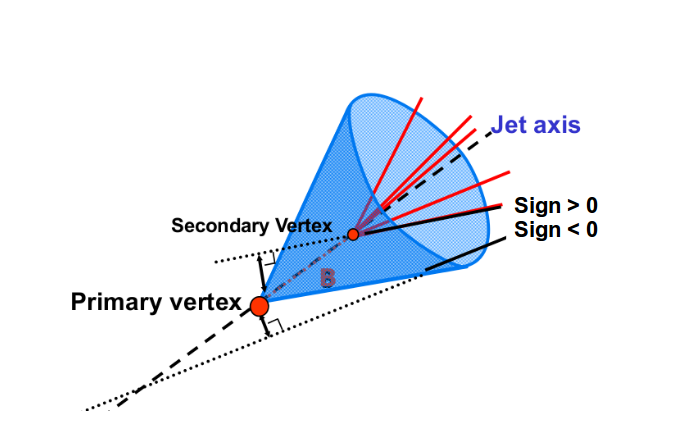
\includegraphics[width=0.7\textwidth]{signedFinal.png}
    \caption{Lifetime sign of tracks. A positive and a negative lifetime signed track is shown.}
    \label{fig:signedIP}
  \end{center}
\end{figure}

%more formal definition of the sign
The lifetime sign can be defined in three-dimensions, acording to the variables $\vec{\pt}_{jet}$, $\vec{\pt}_{trk}$ and $\vec{\Delta r}_{IP} = \vec{r}_{IP} = \vec{r}_{PV}$, the three-dimensional impact parameter of the track with respect to the primary vertex:
%
\begin{equation}
\mbox{sign}_{3D} = \mbox{sign}([\vec{p}_{trk} \times \vec{p}_{jet}]\cdot[\vec{p}_{trk} \times \vec{\Delta r}_{IP} ]).
\end{equation}
%
The computation of the lifetime sign assumes that the jet direction reproduces, up to a good approximation, the $b$-hadron direction. Under this assumption and up to resolution effects both on the jet direction and on the impact parameter and momentum of the track, the lifetime sign of tracks originating from $b$-hadron decays is positive.

The lifetime sign can also be defined on the transverse plane $(x-y)$ or on the longitudinal plane $(r\phi-z)$ by considering respectively the transverse and longitudinal impact parameters (the projections of the three-dimensional impact parameter on the respective planes):
%
\begin{equation}
\mbox{sign}_{r\phi} = \mbox{sign}(\sin(\phi_{jet} - \phi_{trk})\cdot d_{0,trk}); \; \mbox{and} \; \mbox{sign}_{z} = \mbox{sign}((\eta_{jet} - \eta_{trk})\cdot z_{0,trk}).
\end{equation}
%
%PLOTS TO DO
%Distributions for the transverse and longitudinal impact parameter significance are shown in Fig.~\ref{fig:IPsignificance}; the sign of the transverse impact parameter is defined by ``sign$_{r\phi}$'', while the longitudinal impact parameters significance uses ``sign$_z$''.  
Tracks from the fragmentation in light-jets tend to have a signed impact parameter distribution which is symmetric around 0, since they have no correlation with the jet direction. Tracks from $b$- and $c$-hadron decays, as expected, have an asymmetric distribution, with the most significant contribution at positive significances; however a negative tail extending beyond the pure fragmentation contribution is also seen, corresponding to resolution effects and to an eventual mismatch between the $b$-jet and the $b$-hadron directions.
%%%%Extra info
% The definition for sign$_r\phi$ compared to sign$_{3D}$ shields to a more positive shifted distribution for tracks from $b$-hadron decays, and thus potentially a better performance. This result is a bit surprising and seems to indicate that, since the lifetime sign is not taking into account the different errors on the longitudinal and transverse impact parameters, that the longitudinal component of the lifetime sign is diluting the information from the transverse component.


%\begin{figure}[htbp]
%  \begin{center}
%    \includegraphics[width=0.49\textwidth]{IPd0significancesPlots.png}
%    \includegraphics[width=0.49\textwidth]{IPz0significancesPlots.png} 
%    \caption{Impact parameters of tracks associated to light, $c$- and $b$-jets in the transverse and longitudinal direction.}
%    \label{fig:IPsignificance}
%  \end{center}
%\end{figure}

The significance, which gives more weight to tracks measured precisely, is the main ingredient of the tagging algorithms based on impact parameters. Now, the impact parameter significance of all $N$ tracks associated to the jet to tag need to be combined into a single discriminating variable. It is assumed that tracks are uncorrelated, so their probability density functions (PDF), defined based on the transverse and/or longitudinal impact parameter significance distributions for the different hipothesis, are uniquely  defined as a function of the jet flavour. Using a likelihood function defined according to the product of these PDFs, under the hypothesis of uncorrelated tracks, the following likelihood ratio provides the optimal separation, according to Neyman-Person lemma~\cite{1933RSPTA.231..289N}:
%
\begin{equation}
\mbox{LR}(IP_1,IP_2,...,IP_N) = \frac{\prod_{i=1}^N \mbox{PDF}_b(IP_i)}{\prod_{i=1}^N \mbox{PDF}_l(IP_i)}
\end{equation}
%
For convention, the discriminant variable used for $b$-tagging is then defined as:
%
\begin{equation}
\mbox{weight}(IP_1,IP_2,...,IP_N) = \log(\mbox{LR}(IP_1,IP_2,...,IP_N))
\end{equation}
%
Using such a formalism, two impact parameter based $b$-tagging algorithms are constructed, based on the definition of PDF($IP_i$):

\begin{itemize}
\item
1. IP2D: PDF($IP_i$) = PDF($IP_{i,r\phi}$)
\item
2. IP3D:  PDF($IP_i$) = PDF($IP_{i,r\phi}$,$IP_{i,z}$)
\end{itemize}

In the first case the track PDF is one-dimensional, based on the transverse impact parameter significance. In the second case the PDF is based on a two-dimensional histogram of the transverse and longitudinal impact parameter significance. 
%PLOTS OF THE WEIGHTS?

The \textbf{IP3D} is one of the high-performance tagging algorithms supported for the 2011 data-taking, in which input variables are compared to pre-defined smooth Monte Carlo PDFs for both $b$-jet and light jet hypotheses~\cite{ATLAS-CONF-2011-102}.  Prior to the use of these advanced tagger, a simpler tagging algorithm, the \textbf{JetProb}, combining the impact parameter significances of all tracks associated to the jet was devised to be used for early data, being extensively used during 2010~\cite{ATLAS-CONF-2010-091}. 


The impact parameter based algorithm permits to obtain a very good $b$-tagging performance, as will be shown at the end of this chapter. 
%One of the reason of the good performance is that the likelihood method contains implicity, as a prior knowledge in the PDF for $b$-jets, the fraction of tracks expected to arise from fragmentation and the fracion expected to arise from $b$ and $c$-hadron decays. This Method has also a few drawbacks. One is that it does not account for the momentum dependence of the PDFs. And the second is that, while the impact parameter as such is nearly invariant under Lorentz boosts of the $b$-hadron, the error decreases with increasing track $\pt$ and smaller $\eta$. The track-based PDF is thus not invariant neither under a boost of the $b$-quark nor under a boost of its emerging charged particle tracks.This can be cured both by making a track-PDF category dependent. This approach was tried out in ATLAS with significant improvement in performance, but has the disadvantage of increasing the number of free parameters of the likelihood model and making an eventual calibration on data more difficult.
This performance can be improved by using some information from the secondary vertex based vertexing algorithms in two aspects: tracks associated to long lived particle vertices can be removed from the tracks considered for the impact parameter based algorithms; and, the direction between the secondary and the primary vertex positions can be used to improve the reliability of the lifetime sign, subtituting $\vec{p}_{jet}$ with $\vec{r}_{SV} - \vec{r}_{PV} $. The latter improves significantly the estimation of the $b$-hadron direction. Both kinds of information improve the performance of the impact parameter based $b$-tagging algorithms.


\subsubsection{Secondary vertex based $b$-tagging algorithms }

The typical topology of particle decays in a $b$-jet is a decay chain with two vertices, one steaming from the $b$-hadron decay and at least one from $c$-hadron decays. The reconstruction of these secondary vertices is done in an inclusive way, where the number of charged particle tracks originating from the $b$- and $c$-hadron decays is not known a-priori. An exclusive reconstruction of the huge number of different possible $b$-decay modes cannot be performed, the set of selection cuts needed to reconstruct all of them would severely limit the reconstruction efficiency.

Two strategies to detect a secondary decay vertex in $b$-jets are available in ATLAS. The first one is based on the fit of a single geometrical vertex. Even if this hypothesis is not correct, this approximation works well for a large fraction of cases.  The second algorithm is based on a kinematic approach, which assumes that the primary event vertex and the $b$- and the $c$-hadron decay vertices lie approximately on the same line, the flight path of the $b$-hadron. 

The inclusive fit of a single displaced vertex in $b$-jets is based on the VKalVrt~\cite{Kostyukhin:685551} reconstruction package. The main idea of the algorithm implemented in this package is to maximise the $b/c$-hadron vertex detection efficiency, keeping at the same time the probability to find a vertex inside a light jet low. 

The algorithm starts with all tracks associated to the jet and passing a loose cut selection. The vertex search starts with looking for all track pairs and trying to form a two-track vertex. Each track of the pair must have a three-dimensional impact parameter significance with respect to the primary vertex larger than 2$\sigma$ and the sum of these two significances must be larger than 6$\sigma$. To reduce the influence of badly measured tracks, the two-tracks vertices are required to be produced in the direction of flight of the $b$-quark, by requiring the scalar product of $(\vec{r}_{2-track} - \vec{r}_{PV})\cdot \vec{p}_{jet} $ to be positive. Charged particles coming from long lived particles and conversions are not considered for the inclusive $b$-decay vertex fit. All the tracks corresponding to the accepted two-track vertices are used to determined a single secondary vertex.  If the resulting vertex has a very small vertex probability, the track with the highest constribution to the vertex $\chi^2$  is removed from the vertex fit and the vertex fit is repeated until the $\chi^2$ of the vertex fit is good. The result of this procedure is the (eventual) presence of a vertex, its position, and the list of its associated tracks.

The \textbf{SV1} secondary vertex algorithm uses this procedure to reconstruct inclusive secondary vertices. This advanced tagger takes advantage of three of the reconstructed vertex properties: the invariant mass of all tracks associated to the vertex, the ratio of the sum of the energies of the tracks in the vertex to the sum of the energies of all tracks in the jet, and the number of two-track vertices. These variables are combined using a likelihood ratio technique. SV1 relies on a two-dimensional distribution of the two first variables and a one-dimensional distribution of the number of two-track vertices. In addition the distance $\Delta R$ between the jet axis and the line joining the primary vertex to the secondary one is used. 

The three-dimensional decay length significance alone,  signed with respect to the jet direction can be used as a discriminating variable between $b$-jets and light jets: this is the principle of the early data \textbf{SV0} tagger, extensively used as well with the 2010 and 2011 data~\cite{ATLAS-CONF-2010-042}.


As opposed to the algorithm described above, in which the displaced tracks are selected and an inclusive single vertex is obtained, a second algorithm, called \textbf{JetFitter}, is based on a different hypothesis. It assumes that the $b$- and the $c$-hadron decay vertices lie on the same line defined through the $b$-hadron flight path. All charged particle tracks stemming from either decay intersect this $b$-hadron flight axis. This method has the advantage of reconstructing imcomplete topologies, with, for instance, a single track from the $b$-hadron and a single track from the $c$-hadron decay. The fit in this case evaluates the compatibility of the given set of tracks with a $b$-$c$-hadron like cascade topology, increasing the discrimination power against light quark jets.
The lateral displacement of the $c$-hadron decay vertex with respect to the $b$-hadron flight path is small enough not to violate significantly the basic assumption within the typical resolutions of the tracking detector.
The discrimination between $b$-, $c$- and light jets is based on a likelihood using similar variables as in the SV1 tagging algorithm above, and additional
variables such as the flight length significances of the vertices.

\subsubsection{Algorithm combinations and performance}

The IP3D and SV1 tagging algorithms both use the likelihood ratio method, and due to this they can be easily combined: the weights of the individual tagging algorithms are simply summed up. 

The combination of the JetFitter and the IP3D algorithms can be performed using an artificial neural network technique with Monte Carlo simulated training samples and additional variables describing the topology of the decay chain. 

Figure~\ref{fig:btaggingperformance} compares the performance for the various ATLAS $b$-tagging algorithms described in a simulated sample of $t\bar{t}$ events.
It can be seen that by combining the vertexing techniques and the impact parameter information, the IP3D+SV1 and IP3D+JetFitter algorithms can reach very high tagging efficiencies.

 The performance of a $b$-tagging algorithm is usally  measured in terms of the \emph{light-jet rejection} obtained for a given \emph{$b$-jet tagging efficiency}.  Curves are obtained by varying continuously the \emph{operating point} of each tagger, i.e. the cut on its output discriminating variable (weight).  The $b$-jet tagging efficiency,  $\epsilon_b$,  is the fraction of jets labeled as $b$-jets that are properly tagged while the light-jet rejection, defined as $1/\epsilon_{light}$, is the reciprocal of the fraction of jets that are labeled as light jets and are actually tagged incorrectly by the algorithm. 

The labeling procedure used for $b$-tagging is based on the flavor of true quarks: a jet is labeled as a $b$-quark jet if a $b$-quark is found in a cone of size $\Delta R = 0.3$ around the jet direction.  The various labeling hypotheses are tried in this order: $b$ quark, $c$ quark and $\tau$ lepton. When none of these hypotheses are satisfied, the jet
is labeled as a light jet. No attempt is made to distinguish light jets originating from gluons from those originating from quarks at this stage.

\begin{figure}[htbp]
  \begin{center}
      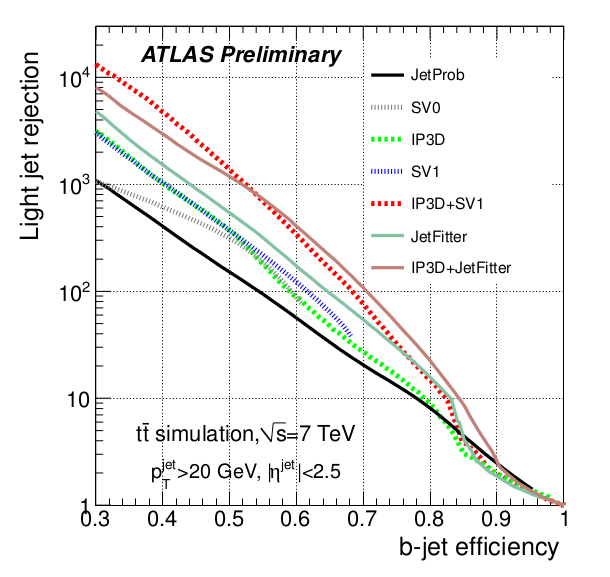
\includegraphics[width=0.7\textwidth]{btaggingperformance.png}
    \caption{Light-jet rejection as a function of the $b$-jet tagging efficiency for the early tagging algorithms (JetProb and SV0) and for the high-performance algorithms, based on simulated $t\bar{t}$ events. }
    \label{fig:btaggingperformance}
  \end{center}
\end{figure}

%By combining the vertexing techniques and the impact parameter information, the IP3D+SV1 and IP3D+JetFitter algorithms can reach very high tagging efficiencies.


\subsubsection{The MV1 tagging algorithm}


The \textbf{MV1} $b$-tagging algorithm is a combined algorithm based on a neural network using the output weights of the IP3D and SV1 algorithms and the JetFitter+IP3D combination as input.  For being the best performing algorithm (better light rejection for the same signal efficiency) it is the recomended tagger for 2011 and 2012 analyses. This is the $b$-tagging algorithm used in this thesis.

%%PLOT OF THE MV1 WEIGHT???????????????
%%TABLA DE LOS SUPPORTED OPERATING POINTS????????

\subsection{$b$-tagging calibration}


In order for $b$-tagging to be used in physics analyses, the efficiency with which a jet originating from a $b$-quark is tagged by a $b$-tagging algorithm needs to be measured in data.  Morover, an appropriate description of the $b$-tagging efficiencies based on measurements with data is essential for correctly modelling the measurements in Monte Carlo simulation . A second necessary piece of information is the probability of mistakenly tagging a jet originating from a light-flavour ($u$-, $d$-, $s$-quark or gluon) jet as a $b$-jet, referred to as the mistag rate. The $b$-tagging ``calibration'' includes both the measurement of the mis-tag rates and $b$-tagging efficiency.


The measurements of the $b$-tag efficiency and mistag rate are provided in the form of jet $\pt$- and $\eta$-dependent scale factors that correct the $b$-tagging performance in simulation to that observed in data.  The scale factors are defined as the ratio of the $b$-tag efficiency or mistag rate in data and simulation:
%
\begin{equation}
\kappa_{\epsilon_b}^{data/sim}  = \frac{\epsilon_b^{data}}{\epsilon_b^{sim}}, \; \;   \kappa_{\epsilon_l}^{data/sim}  = \frac{\epsilon_l^{data}}{\epsilon_l^{sim}},
\end{equation}
%
where $\epsilon_b^{sim}$ and $\epsilon_l^{sim}$ are the fractions of $b$- and light-flavour jets which are tagged in simulated events, %an inclusive sample of simulated $t\bar{t}$ events,
 with the jet flavour defined by matching to generator level partons as defined in the previous section. %The measured $b$-tag efficiencies and mistag rates will depend on the jet transverse momentum $\pt$ and the pseudorapidity $\eta$.  %They also depend on other quantities such as the fraction of jets in the sample originating from gluons. An advantage of providing the calibration results in the form of scale factors is that even though samples with different event topologies can have slightly different $b$-tag efficiencies or mistag rates, the data-to-simulation scale factors are likely to be valid.

In physics analyses, these $\pt$-dependent scale factors are then applied as weights to the jets in Monte Carlo simulation, to reproduce the $b$-tagging performance in data.


The main $b$-tagging efficiency calibration methods, the so called \emph{system8} and $p_{rel}$ methods are described in detail in ref~\cite{ATLAS-CONF-2011-089}.% based on an integrated luminosity of L = 4.7 fb−1 collected in 2011. 
These measurements are based on a sample of jets with muons inside, where the muons are serving as a reference $b$-tagging algorithm to obtain a $b$-jet sample on which the calibrations can be performed. 
At the LHC, the large $t\bar{t}$ production cross section of $\sigma_{t\bar{t}} = 177 ± 3(\mbox{stat.})+8 (\mbox{sys.}) ± 7(\mbox{lum.})$~pb~\cite{ATLAS-CONF-2012-024} offers an alternative source of events enriched in $b$-jets. % This distinctive topology with high pT leptons, multiple jets, and large missing transverse momentum provides highly selective trigger objects and is relatively easy to reconstruct. With the large integrated luminosity of 4.7 fb−1 collected during 2011, the methods based on tt selections have become competitive for the first time. In addition to providing b-tagging calibration measurements in an inclusive b-jet sample rather than a sample of semileptonic b-jets. In addition to providing b-tagging calibration measurements in an inclusive b-jet sample rather than a sample of semileptonic b-jets, these methods  methods also allow to extend the calibrated pT range. Furthermore, the tt environment of high jet  multiplicity and high pT b-jets is more similar to the final states to which b-tagging is applied than the semileptonic jet sample.
Calibrations using samples of $t\bar{t}$ events have been obtained for SV0, IP3D+SV1, JetFitter and MV1 $b$-tagging algorithms~\cite{ATLAS-CONF-2012-097}. All these algorithms provide an output weight $w$, discriminating between $b$-jets and non-$b$-jets. Lower values of $w$ are assigned to $c$- and light-flavour jets, whereas the purity of $b$-jets increases with $w$. For each $b$-tagging algorithm a set of operating points, corresponding to a certain $w$ cut value, are defined and calibrated:

\begin{itemize}
\item
SV0: $\epsilon_b^{sim} =$ 50\%
\item
IP3D+SV1: $\epsilon_b^{sim} =$ 60\%, $\epsilon_b^{sim} =$ 70\%, $\epsilon_b^{sim} =$ 80\%
\item
JetFitter: $\epsilon_b^{sim} =$ 57\%, $\epsilon_b^{sim} =$ 60\%,  $\epsilon_b^{sim} =$ 70\%, $\epsilon_b^{sim} =$ 80\%
\item
MV1: $\epsilon_b^{sim} =$ 60\%, $\epsilon_b^{sim} =$ 70\%, $\epsilon_b^{sim} =$ 75\%, $\epsilon_b^{sim} =$ 85\%
\end{itemize}
%
where  $\epsilon_b^{sim}$ is the nominal $b$-tagging efficiency derived from an inclusive sample of simulated $t\bar{t}$ events.

%http://cdsweb.cern.ch/record/1435194
The mistag rate is measured in data using two methods, both based on an inclusive sample of jets, referred to as the $negative tag$ and $sv0mass$ methods~\cite{ATLAS-CONF-2012-040}. The first method uses the invariant mass spectrum of tracks associated with reconstructed secondary vertices to separate light and heavy-flavour jets, and the other is based on the rate at which secondary vertices with negative decay length, or tracks with negative impact parameter, are present in the data.


Currently, there is no explicit measurement of the $c$-tag efficiency available in ATLAS. As both the
$b$- and $c$-tag efficiencies are dominated by decays of long-lived heavy flavour hadrons, they are expected to show a similar behaviour. In general, for physics analyses, it is thus assumed that the scale factor is the same for $b$- and $c$-jets. However, to take into account possible deviations from this assumption, the systematic uncertainty for the $c$-tag efficiency scale factor is inflated by a factor of two, which is considered to be a conservative choice based on simulation studies. In the future, the $c$-tag efficiency will be measured in dedicated analyses.



%\subsection{Pile-up}
%Out-of-time pile-up events ($pp$ collisions from neighboring bunches in the same train) also generate calorimeter activity and consequently extra jets. However, given the time resolution of the Inner Detector, and since the $b$-tagging algorithms reject jets with no track associtaed to them, the contribution of the out-of-time pile-up for this analysis is expected to be negligible.
 
%
%%%%%%%%%%%%%%%%%%%%%%%%%%%%%%%%%%%%%%%%%%%%%%%%%%%%%%%%%%%%%%%%%%%%%%%%%%%%%%%
% Kinematic differences between single and double $B$-hadron jetsDouble 
%%%%%%%%%%%%%%%%%%%%%%%%%%%%%%%%%%%%%%%%%%%%%%%%%%%%%%%%%%%%%%%%%%%%%%%%%%%%%%%
%
\chapter{Kinematic differences between single and double $B$-hadron jets}

%------------------------------------------------------------------------
%\section{Introduction}\label{sec:gbbintro}
%------------------------------------------------------------------------

%The purpose of this note is to describe the development of an algorithm to identify the $b$-jet flavor structure of single jets.  In particular, the proposed technique attempts to identify if the $b$-jet substructure is consistent with the decay of one or two $B$-hadrons within a single jet. There are two different strategies to approach this problem. One approach is to attempt to reconstruct multiple vertices originating from the decay of long-lived $B$-hadrons\cite{CDFAzimutalCorrelation}. % or use jet shape/substructure information. The former approach has low efficiency due to the double $b$-tag requirement that goes as the square of the $b$-tagging efficiency\cite{CDFAzimutalCorrelation}.

%In the present analysis we are exploring a different way to tag double $B$-hadron jets that does not rely on explicitly finding vertices but uses the jet shape/substructure information. Eventually, the goal should be to combine both approaches.

%------------------------------------------------------------------------
\section{Data and Monte Carlo samples}\label{sec:Simulation}
%------------------------------------------------------------------------


The tagging technique presented in this thesis relies on Monte Carlo predictions for the signal (single $b$) or background (merged $b$) hypotheses. The accuracy of the simulation is validated with data by comparing the distributions of the different variables explored.

Samples of jet events from proton-proton collision processes are simulated with {\sc Pythia8}~\cite{PYTHIA8} event generator using a $2\rightarrow 2$ matrix element at leading order in the strong coupling to model the hard subprocess, and $\pt$-ordered parton showers are utilized to model additional radiation in the leading-logarithmic approximation~\cite{Pythia_partonshowers}. Multiple parton interactions~\cite{Pythia_mpi}, as well as fragmentation and hadronisation based on the Lund string model~\cite{Lund_string_model} are also simulated.
%The proton parton distribution function (PDF) set used is the modified leading-order PDF set MRST LO*~\cite{}. 
The ATLAS MC11 tune of the soft model parameters was used~\cite{Pythia_MC11tune}.
In order to have sufficient statistics over the entire $\pt$ spectrum, eight samples were generated with different thresholds of the hard-scattering partonic transverse momentum $\hat{p}_T$. Events from different samples were mixed taking into account their respective production cross sections.

%After the event generation, the events are passed through a full {\sc Geant4}~\cite{GEANT4} detector simulation with a detailed description of the geometry and the material of the ATLAS experiment, and %QGSP$\_$BERT~\cite{QGSP, BERT} asthe set of processes describing the hadronic interactions.
%using Bertini Cascades~\cite{QGSP, BERT} for the modeling of interactions of high energy hadrons. 
The {\sc Geant4}~\cite{GEANT4} software toolkit within the ATLAS simulation framework~\cite{ATLASSimulation} propagates the generated particles through the ATLAS detector and simulates their interactions with the detector material. The energy deposited by particles in the active detector material is converted into detector signals in the same format as the detector read-out. Finally the Monte Carlo generated events are processed through the trigger simulation package of the experiment, and are reconstructed and analyzed with the same software as for the real data.
The simulated data sample used for the analysis %(MC11b)
gives an accurate description of the pile-up content and detector conditions for the full 2011 data-taking period. 

The data samples employed correspond to proton-proton collisions at $\sqrt{s}=7$ TeV delivered by the LHC and recorded by ATLAS between May and November 2011, with the LHC running with 50~ns bunch spacing, and bunches organized in bunch trains. Only data collected during stable beam periods in which all sub-detectors were fully operational are used.  After the application of the data quality selection, % the total integrated luminosity is about  4.7 fb$^{-1}$.  
the surviving data corresponds to an integrated luminosity of 4.7~fb$^{-1}$. The LHC performance steadily improved during 2011. In particular  the average number of minimum-bias pile-up events, originating from collisions of additional protons in the same bunch as the signal collision, grew from from 3 to 20. This fact will be of importance when discussing the selection of discriminating variables.  
%the average number of interactions per bunch crossing throughout the data-taking period considered was approximately $3 \leq  \mu \leq 8$ until summer 2011, with a global average for this period of $\mu \approx 6$. Starting in August 2011 and lasting through the end of the proton run, $\mu$ ranged from approximately 5 to 17, with an average of about 12. 

For the study of systematic effects and for result comparison, other Monte Carlo samples were utilised. Results were produced with the {\sc herwig}++  generator~\cite{Herwig} and with {\sc Pythia8} using the Perugia tune~\cite{Perugia}. The former is based on the event generator {\sc herwig}, but redesigned in the $C$++ programming language. The generator contains a few modlleing improvements. It also uses angular-ordered parton showers, but with an updated evolution variable and a better phase space treatment. Hadronisation is perfromed using the cluster model. The underlying event and soft inclusive interactions are described using a hard and soft multiple partonic interactions model~\cite{Bahr:2008dy}. The Perugia tune is an independent tune of {\sc pythia} with increased final state radiation to better reproduce the jet shapes and hadronic event shapes using LEP and {\sc tevatron} data. In addition, paramteres sensitive to the production of particles with strangeness and related to jet fragmentation have been adjusted.


%en realidad voy a referir al capitulo donde describo los distintos MC generators y voy a decir
%The Monte Carlo event generators discussed in Section... are used here. 
%Pythia, pythia with the Perugia tune and herwig++ where these are used both for the simulation of the hard 2-2 process as well as for the parton shower, underlying event, and hadrnisation models.


%------------------------------------------------------------------------
\section{Event and object selection}\label{sec:EventSelection}
%------------------------------------------------------------------------

%In this section we examine the procedure for event selection and the conditions that the calorimeter jets must satisfy in order to be considered.

%%% The following was taken from this BTagging note, https://cdsweb.cern.ch/record/1435194
%%% from 2012! 
The event sample for this analysis was collected  using a logical OR of single jet triggers which select events with at least one jet with transverse energy above a given threshold at the highest trigger level. The ATLAS Trigger system uses three consecutive trigger levels. At the hardware Level 1 and local software Level 2, cluster-based jet triggers are used to select events. The Level 3, the so-called Event Filter, runs  the offline anti-$k_t$ jet finding algorithm with $R = 0.4$ on topological clusters over the complete calorimeter.  At this stage, the transverse energy thresholds, expressed in GeV, are: 20, 30, 40, 55, 75, 100, 135, 180. These triggers reach an efficiency of 99\% for events having the leading jet with an offline energy higher than the corresponding trigger thresholds by a factor ranging between 1.5 and 2. The triggers with the lowest $\pt$ thresholds were prescaled by up to five orders of magnitude, and typically the same jet trigger is prescaled ten times more in the later data taking periods compared to the early ones. %The offline event selection consists of requiring at least one primary vertex candidate to have 5 or more tracks. 

%Only events with exactly two B hadrons were considered.

%Monte Carlo jets belong to the QCD simulation described in section~\ref{sec:Simulation}.

The offline event selection requires at least one primary vertex candidate with 5 or more tracks. All jets, with transverse momentum between 40 and 480~GeV,  %, reconstructed with the anti-$k_t$ $R=0.4$ algorithm built from topological clusters, 
were required to be in a region with full tracking coverage, $|\eta_{jet}|<2.1$, and they were classified in eight $\pt$ bins chosen such as to match the jet trigger 99\% efficiency thresholds (in GeV): 40, 60, 80, 110, 150, 200, 270, 360.  %The trigger strategy is detailed in Table~\ref{tab:trigger}. 
 Only jets tagged as $b$-jets using the MV1 $b$-tagging algorithm at the 60\% efficiency working point were considered. $b$-tagged jets with close-by jets ($\Delta R < 0.8$) with $\pt$ higher than 7~GeV at electromagnetic scale were not included in the analysis. Unless otherwise indicated, performance plots are shown for one medium  $\pt$ bin (80 to 110~GeV) and one high $\pt$ bin (200 to 270~GeV).


In the case of MC the reconstructed $b$-tagged jets were further classified into single and merged $b$-jets based on truth Monte Carlo information. A $B$-hadron is considered to be associated to a jet if the $\Delta R$ distance in $\eta-\phi$ space between the direction of the hadron and the jet axis is smaller than 0.4. Jets were labeled as merged (single) $b$-jets if they contain two (only one) $B$-hadron.%\footnote[2]{Another approach is to match particles using the 'active area' of the jet, defined with the concept of ghost-particles but utilizing true particles as ghost constituents\cite{CatchmentArea}. This procedure will be implemented in a future version of this analysis.}.

 


%\begin{table}
%\renewcommand{\arraystretch}{1.3}
%\centering
%{\small
%\begin{tabular}{|   c   |   c   |   c   |}
%\hline $\pt$ (GeV) & Run 177531 - 187109 & Run $>$ 187109 \\  \hline
%%(30,40)     & EF\_j15\_a4\_EFFS  OR  EF\_j10\_a4\_EFFS  & EF\_j15\_a4tc\_EFFS OR  EF\_j10\_a4tc\_EFFS   \\ \hline \hline
%(40,60)     & EF\_j20\_a4\_EFFS  OR  EF\_j15\_a4\_EFFS  & EF\_j20\_a4tc\_EFFS OR  EF\_j15\_a4tc\_EFFS   \\ 
%(60,80)     & EF\_j30\_a4\_EFFS  OR  EF\_j20\_a4\_EFFS  & EF\_j30\_a4tc\_EFFS OR  EF\_j20\_a4tc\_EFFS   \\ 
%(80,110)    & EF\_j40\_a4\_EFFS  OR  EF\_j30\_a4\_EFFS  & EF\_j40\_a4tc\_EFFS OR  EF\_j30\_a4tc\_EFFS   \\ 
%(110,150)   & EF\_j55\_a4\_EFFS  OR  EF\_j40\_a4\_EFFS  & EF\_j55\_a4tc\_EFFS OR  EF\_j40\_a4tc\_EFFS   \\ 
%(150,200)   & EF\_j75\_a4\_EFFS  OR  EF\_j55\_a4\_EFFS  & EF\_j75\_a4tc\_EFFS OR  EF\_j55\_a4tc\_EFFS   \\ 
%(200,270)   & EF\_j100\_a4\_EFFS OR  EF\_j75\_a4\_EFFS  & EF\_j100\_a4tc\_EFFS OR  EF\_j75\_a4tc\_EFFS  \\ 
%(270,360)   & EF\_j135\_a4\_EFFS OR  EF\_j100\_a4\_EFFS & EF\_j135\_a4tc\_EFFS OR  EF\_j100\_a4tc\_EFFS \\ 
%(360,480)   & EF\_j180\_a4\_EFFS OR  EF\_j135\_a4\_EFFS & EF\_j180\_a4tc\_EFFS OR  EF\_j135\_a4tc\_EFFS \\ %\hline \hline
%$>$480     & EF\_j240\_a4\_EFFS OR  EF\_j180\_a4\_EFFS & EF\_j240\_a4tc\_EFFS OR  EF\_j180\_a4tc\_EFFS \\
%\hline
%\end{tabular}
%}
%\caption{The \pt\ bins used in the present analysis and the respective triggers the must satisfy.}
%\label{tab:trigger}
%\end{table}



%------------------------------------------------------------------------
%\section{Track selection }\label{sec:TrackSelection}
%------------------------------------------------------------------------

It is important to select genuine tracks belonging to jets. Only tracks located  within a cone of radius $\Delta R(jet^{\rm reco},\rm track) \leq 0.4$ around the jet axis were considered. %\footnote[2]{In a future version of the study the concept of ghost-particles\cite{CatchmentArea} can be applied in the track-to-jet assignment using tracks as ghost constituents.}.
  Cuts on $p_{\rm{T}}^{\rm{trk}}>1.0$~GeV and the $\chi^2$ of the track fit, $\chi^2/{\it ndf}<3$, are applied. % as a minimum starting point. 
 In addition, tracks are required to have a total of at least seven precision hits (pixel or micro-strip) in order to guarantee at least 3 $z$-measurements. Tracks are also required to fulfill cuts on the transverse and longitudinal impact parameters at the perigee to ensure that they arise from  the primary vertex. As cutting on impact parameter (IP) significance might be detrimental for $b$-jets, where large IP values are expected, the relaxed cuts were used, $|IP_{xy}|<2$~mm, and $|IP_{z}\sin\theta|<2$~mm, with $\theta$ being the polar angle measured with respect to the beam axis. %This, however, might still be too tight for $b$-jets.



%------------------------------------------------------------------------
%\section{Kinematid differences between single $b$- and merged $b\bar{b}$-jets}\label{sec:gbbKine}
\section{Preliminary studies in standalone {\sc pythia} generator}\label{sec:gbbKine}
%------------------------------------------------------------------------ 


A small set of dijet events was generated using {sc pythia}. With the help of fastjet~\cite{fastjet}, anti-$k_t$ jets with distance parameters $R$ of 0.4 and 0.6 were built using as inputs:

\begin{itemize}\addtolength{\itemsep}{-0.4\baselineskip}
\item
all stable particles
\item
charged stable particles
\item 
0.1 $k_t$ jets, using all particles 
\item 
0.1 $k_t$ jets, using charged particles 
\end{itemize}

The labeling was done in the same procedure as in the Full ATLAS Monte Carlo analysis.

Figures~\ref{fig:pythiaTrkWidthAnkt4and6} to~\ref{fig:CorrTau1Tau2DRkt} show the distributions and correlations of some of the tracking variables, for single and merged $b$-jets, in bins of the jet $\pt$.


\begin{figure}[tp]
\centering
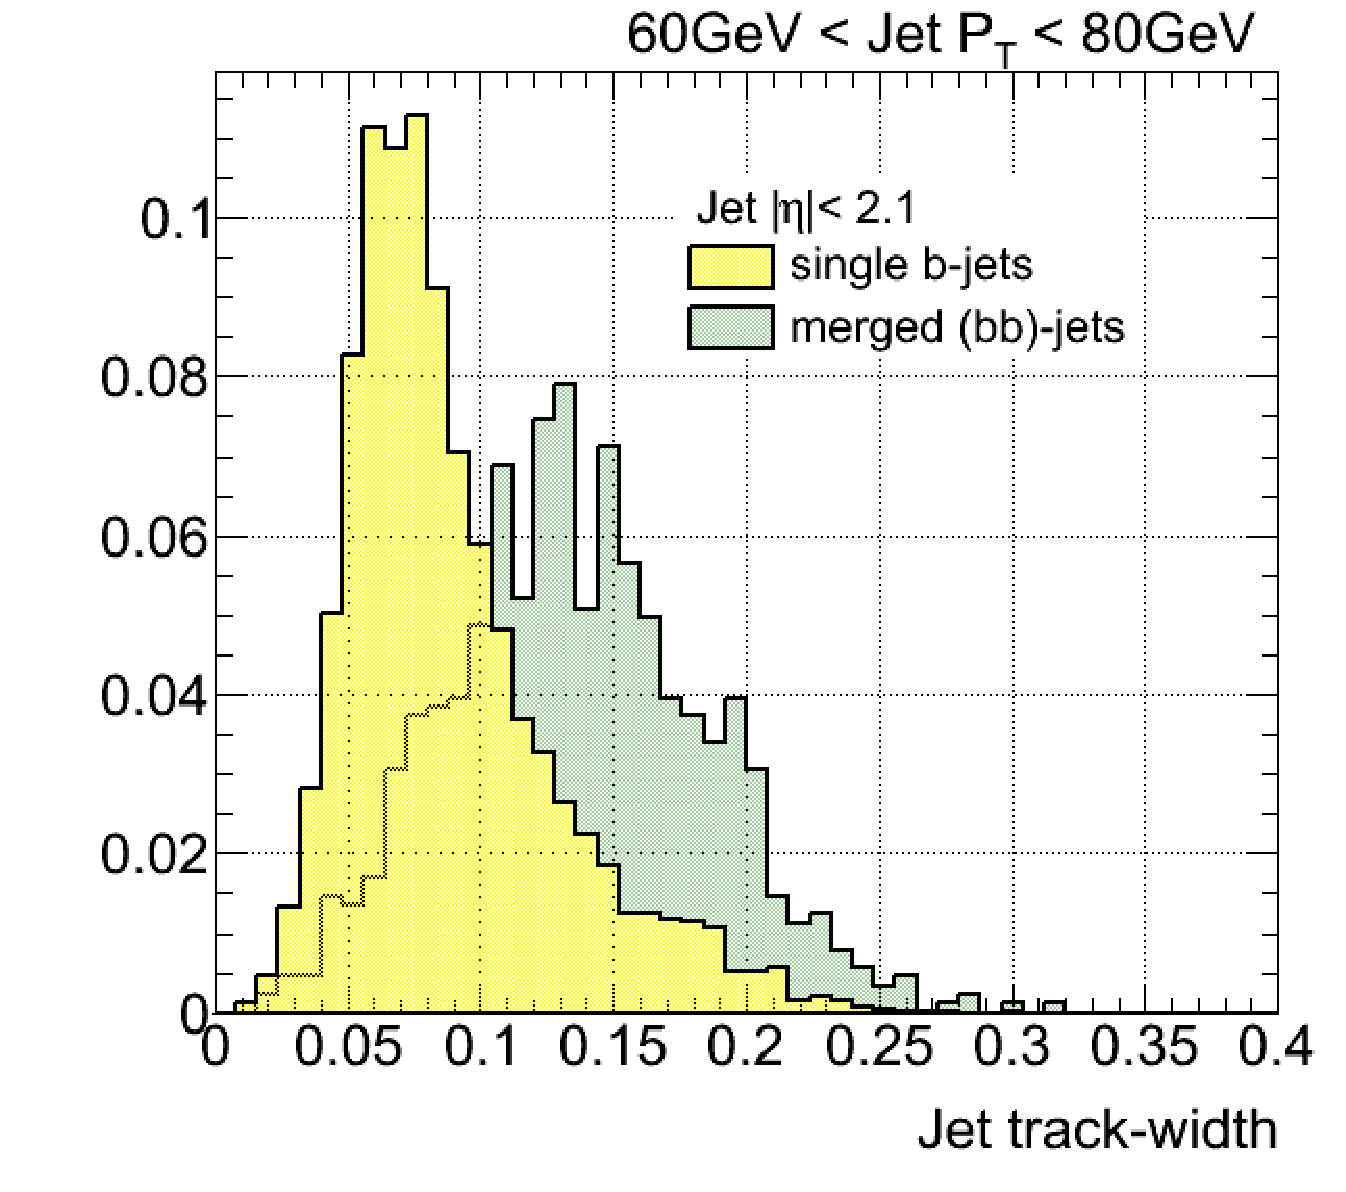
\includegraphics[width=0.49\textwidth]{FIGS/TEMPFigs/PythisStandalone/Antikt4/allparticles/trkWidth060.pdf}
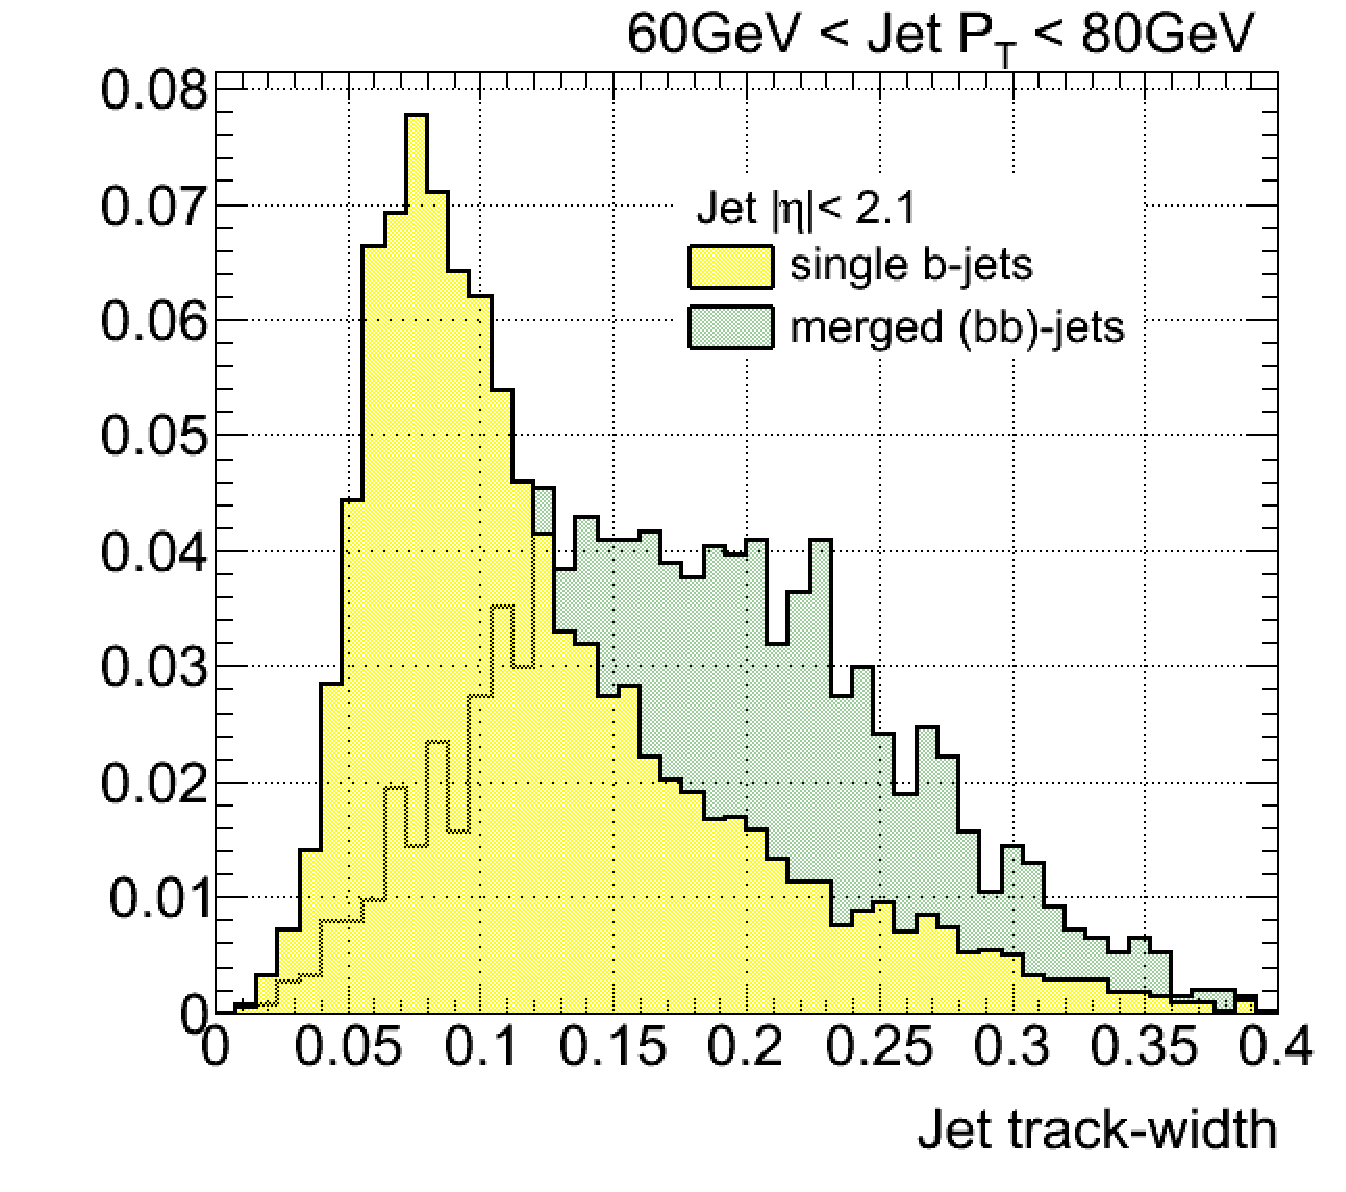
\includegraphics[width=0.49\textwidth]{FIGS/TEMPFigs/PythisStandalone/Antikt6/allparticles/trkWidth060.pdf}
\caption{Distribution of track-jet width in anti-$k_T$ 0.4 (left) and 0.6 (right) jets, for single and merged $b$-jets between 60~GeV to 80~GeV. Jets were built using all stable particles in the simulation.}
\label{fig:pythiaTrkWidthAnkt4and6}
\end{figure}

\begin{figure}[tp]
\centering
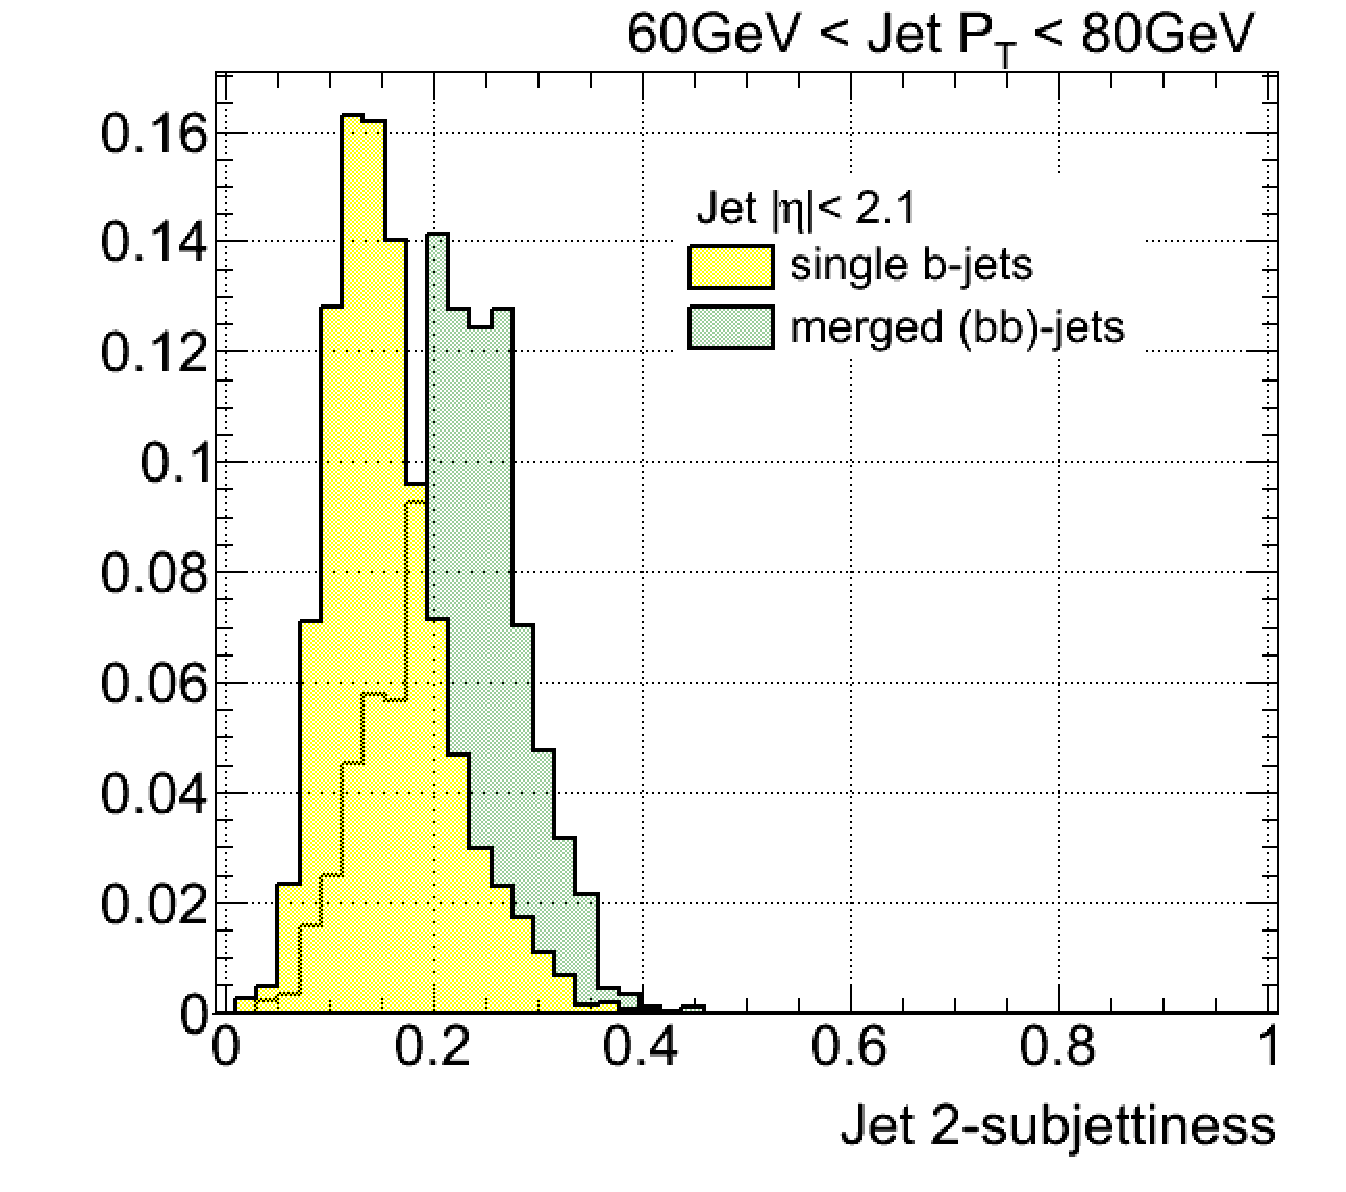
\includegraphics[width=0.49\textwidth]{FIGS/TEMPFigs/PythisStandalone/Antikt4/allparticles/Tau2060.pdf}
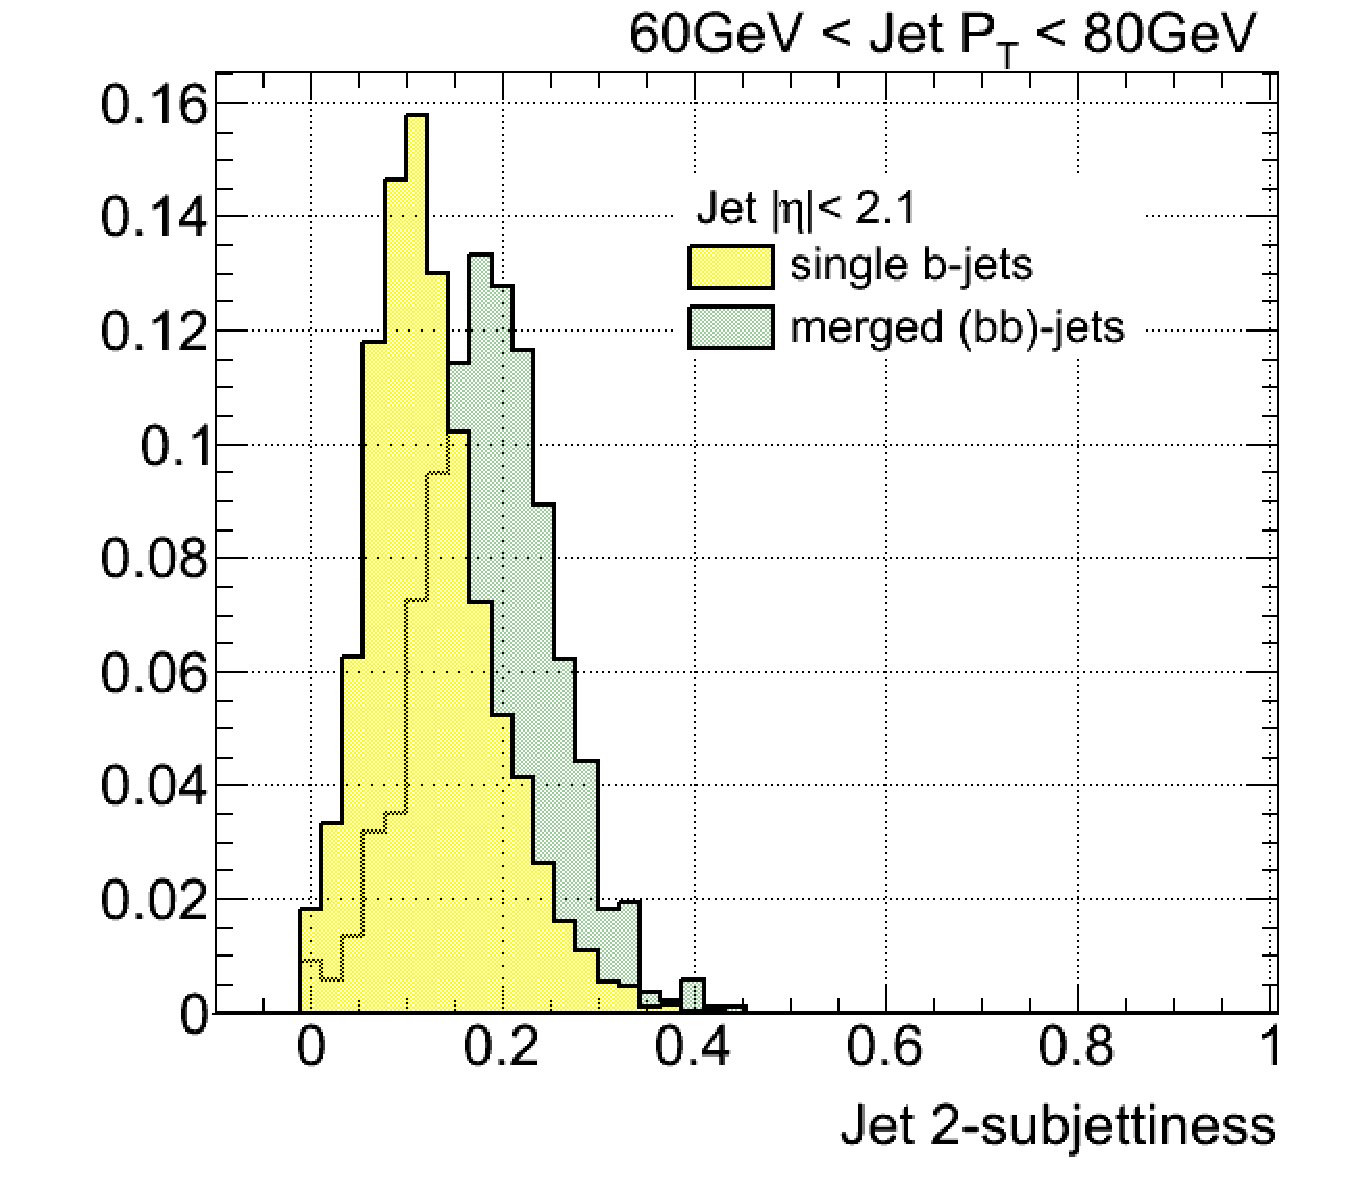
\includegraphics[width=0.49\textwidth]{FIGS/TEMPFigs/PythisStandalone/Antikt4/chargedparticles/Tau2060.pdf}
\caption{Distribution of $\tau_2$ in anti-$k_T$ 0.4 jets, for single and merged $b$-jets between 60~GeV to 80~GeV. Jets were built using all stable particles (left) and charged particles only (right).}
\label{fig:pythiaTau2AllandCharged}
\end{figure}

\begin{figure}[tp]
\centering
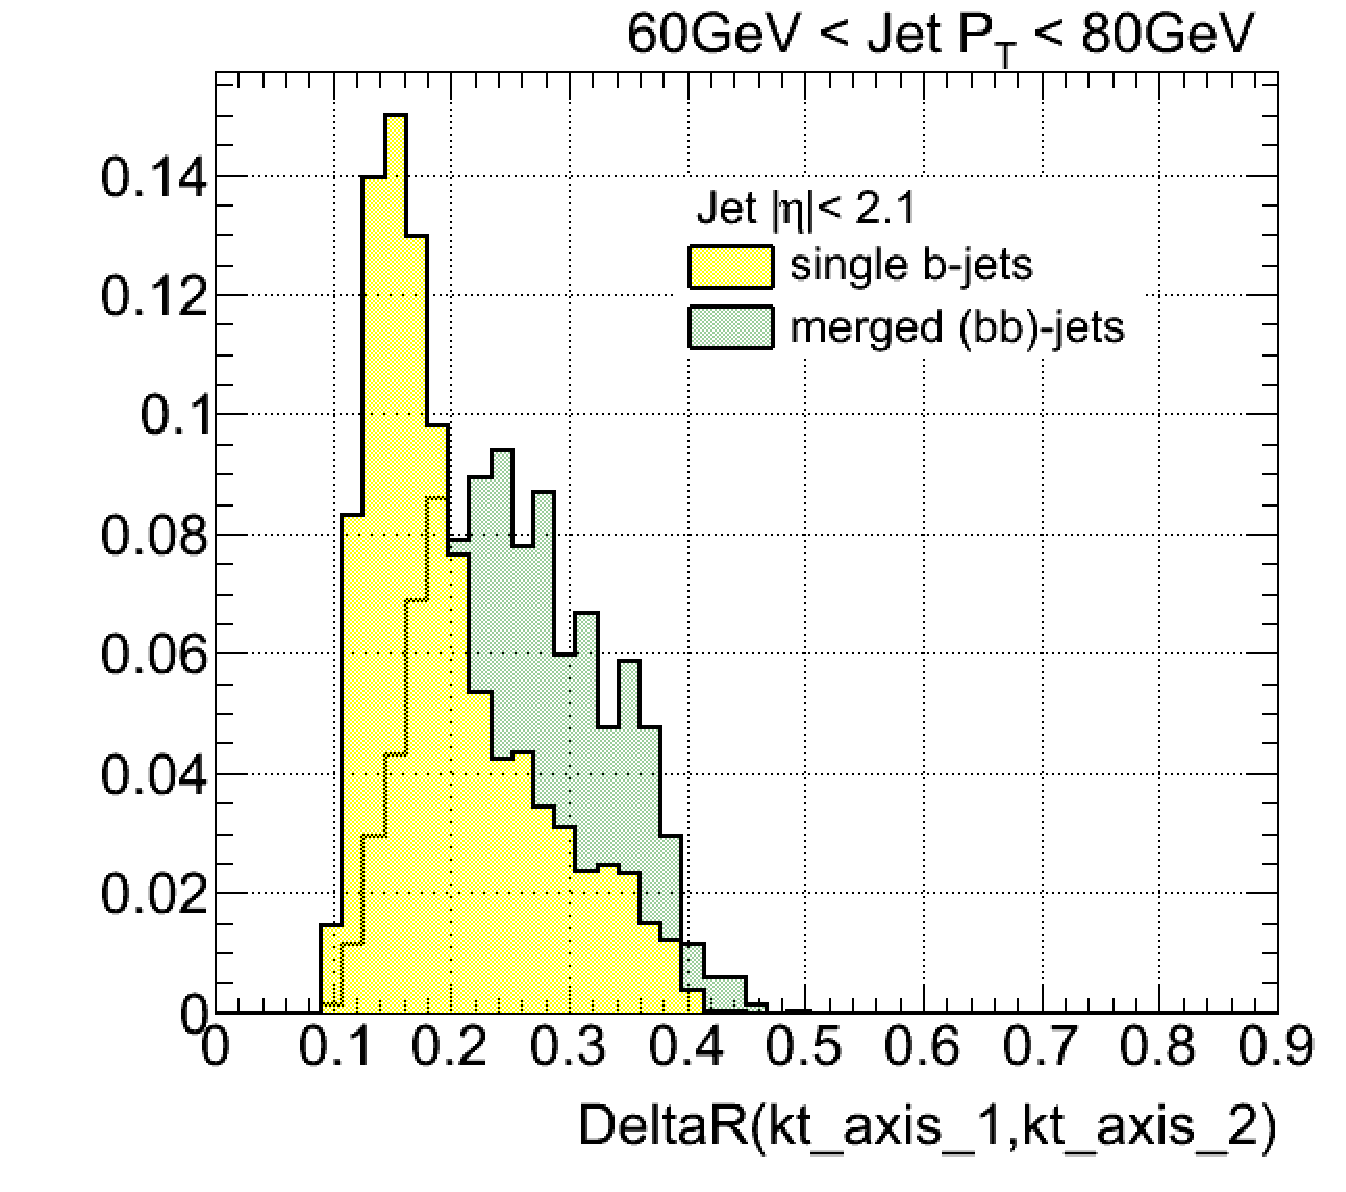
\includegraphics[width=0.49\textwidth]{FIGS/TEMPFigs/PythisStandalone/Antikt4/minijets/DRkt2axes060.pdf}
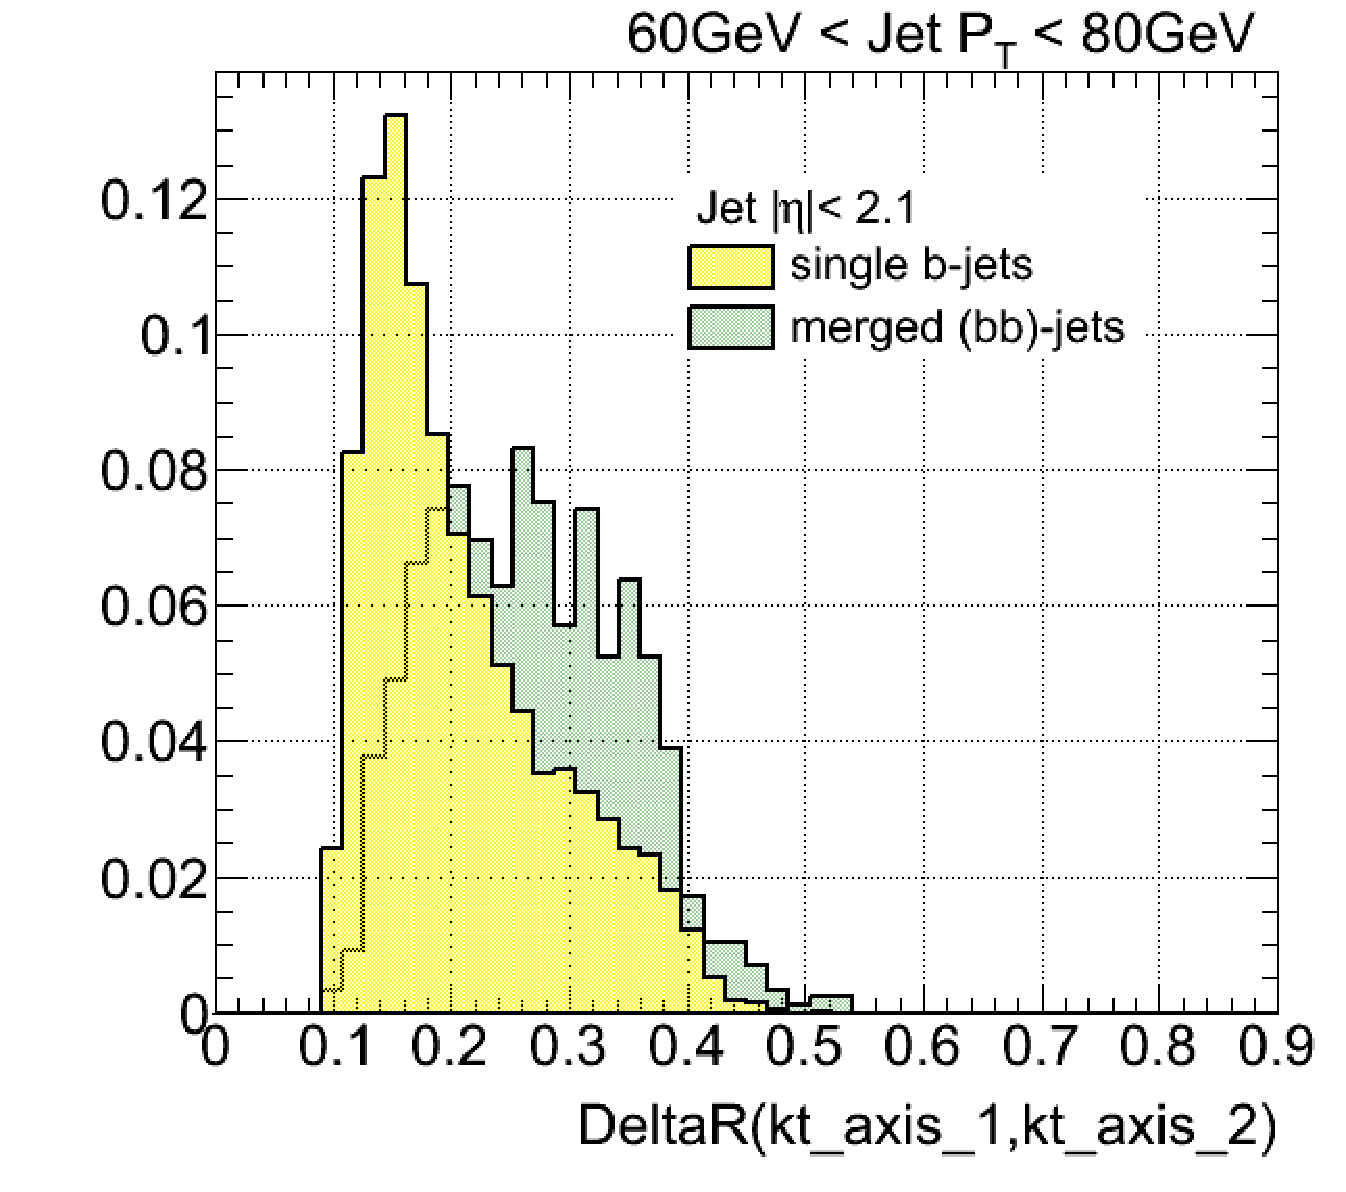
\includegraphics[width=0.49\textwidth]{FIGS/TEMPFigs/PythisStandalone/Antikt4/chargedminijets/DRkt2axes060.pdf}
\caption{Distribution of $\Delta R$ between the axes of two $k_T$ subjets in anti-$k_T$ 0.4 jets, for single and merged $b$-jets between 60~GeV to 80~GeV. Jets were built using 0.1 $k_t$ jets from all stable particles (left) and charged particles only (right).}
\label{fig:pythiaDRktAllJetandChargedJet}
\end{figure}

\begin{figure}[tp]
\centering
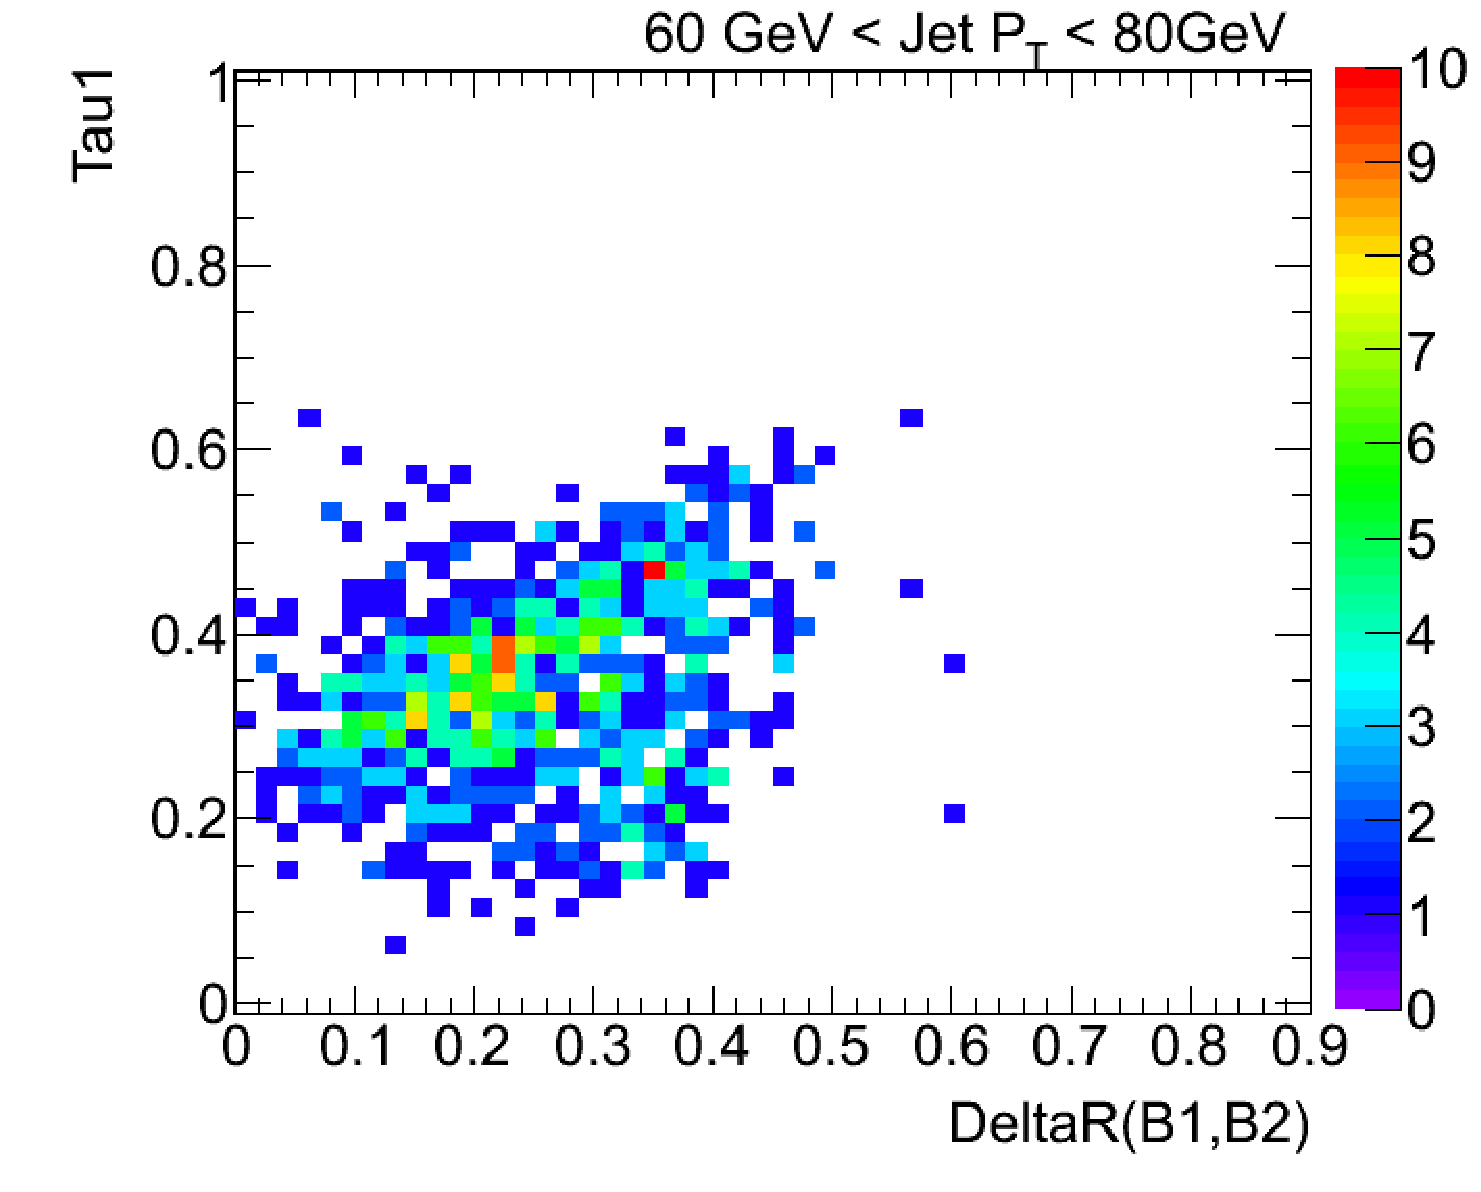
\includegraphics[width=0.49\textwidth]{FIGS/TEMPFigs/PythisStandalone/Antikt4/allparticles/Tau1DeltaRCorr_PT60.pdf}
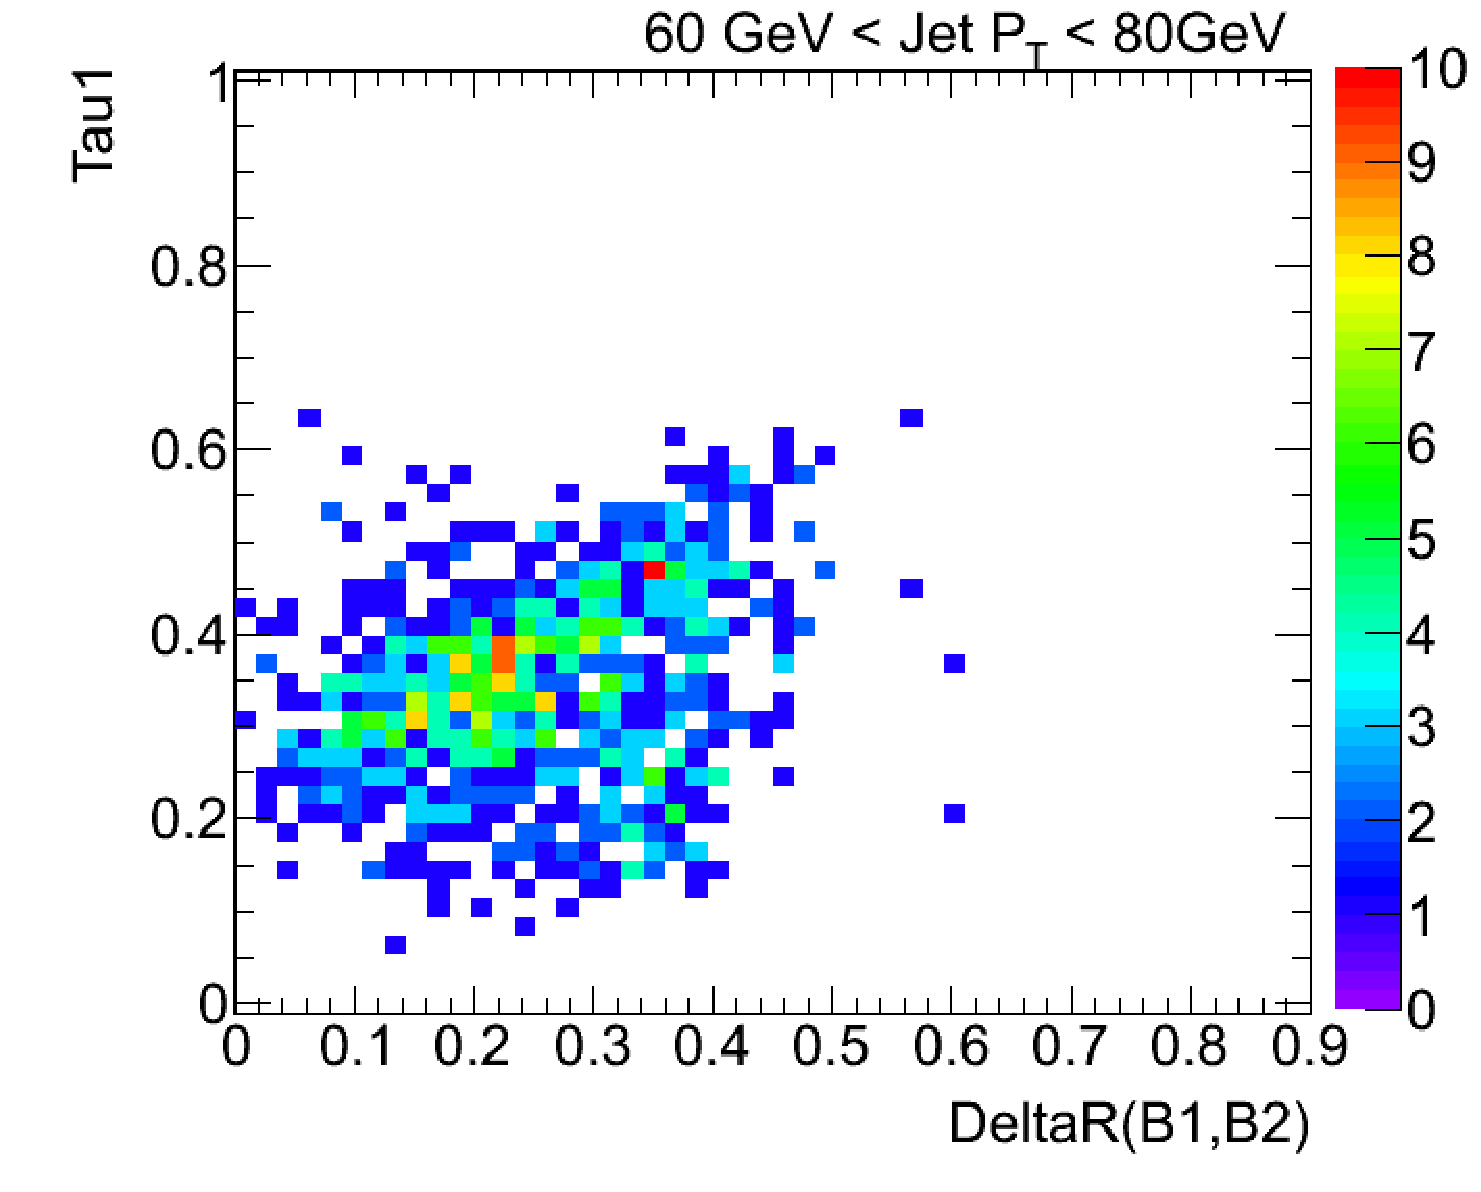
\includegraphics[width=0.49\textwidth]{FIGS/TEMPFigs/PythisStandalone/Antikt4/allparticles/Tau1DeltaRCorr_PT60.pdf}
\caption{Correlation between $\tau_1$ (left) and $\tau_2$ (right) and the $\Delta R$ between the $B$-hadrons in merged anti-$k_T$ 0.4 jets  between 60~GeV to 80~GeV. Jets were built using all stable particles.}
\label{fig:CorrTau1Tau2DRBB}
\end{figure}

\begin{figure}[tp]
\centering
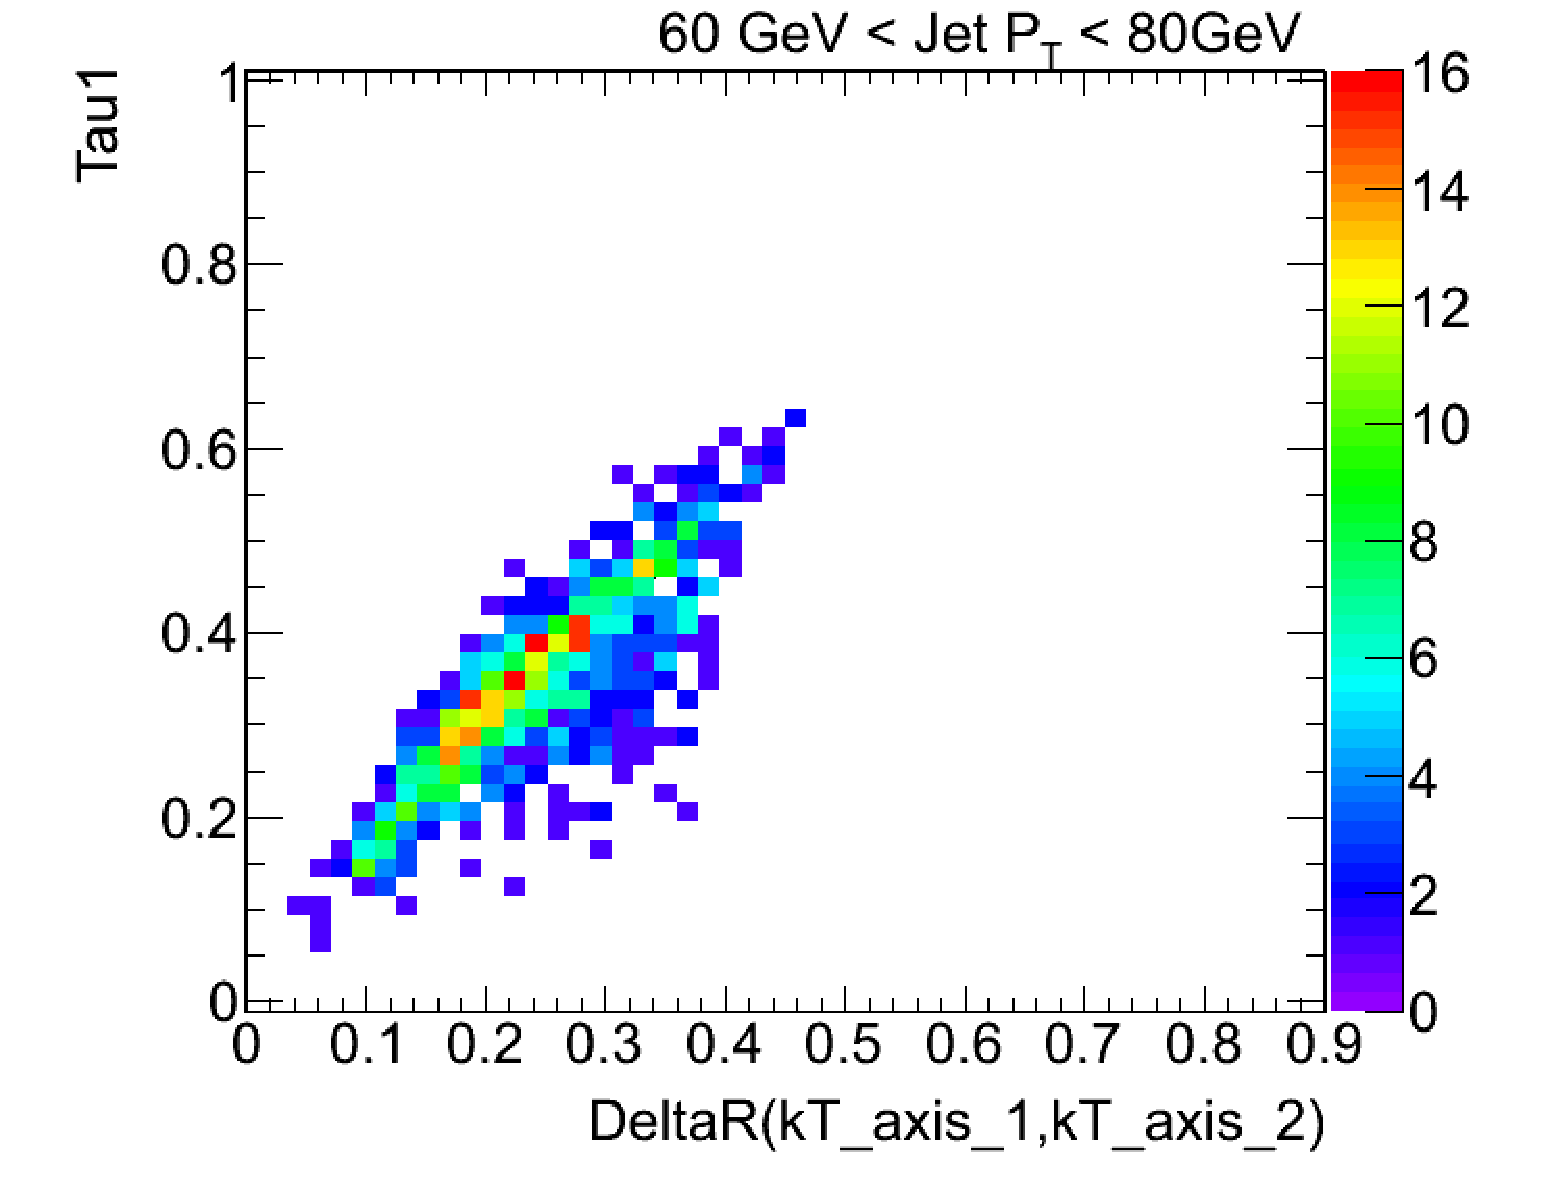
\includegraphics[width=0.49\textwidth]{FIGS/TEMPFigs/PythisStandalone/Antikt4/allparticles/Tau1DRkT2axesCorr_PT60_merged.pdf}
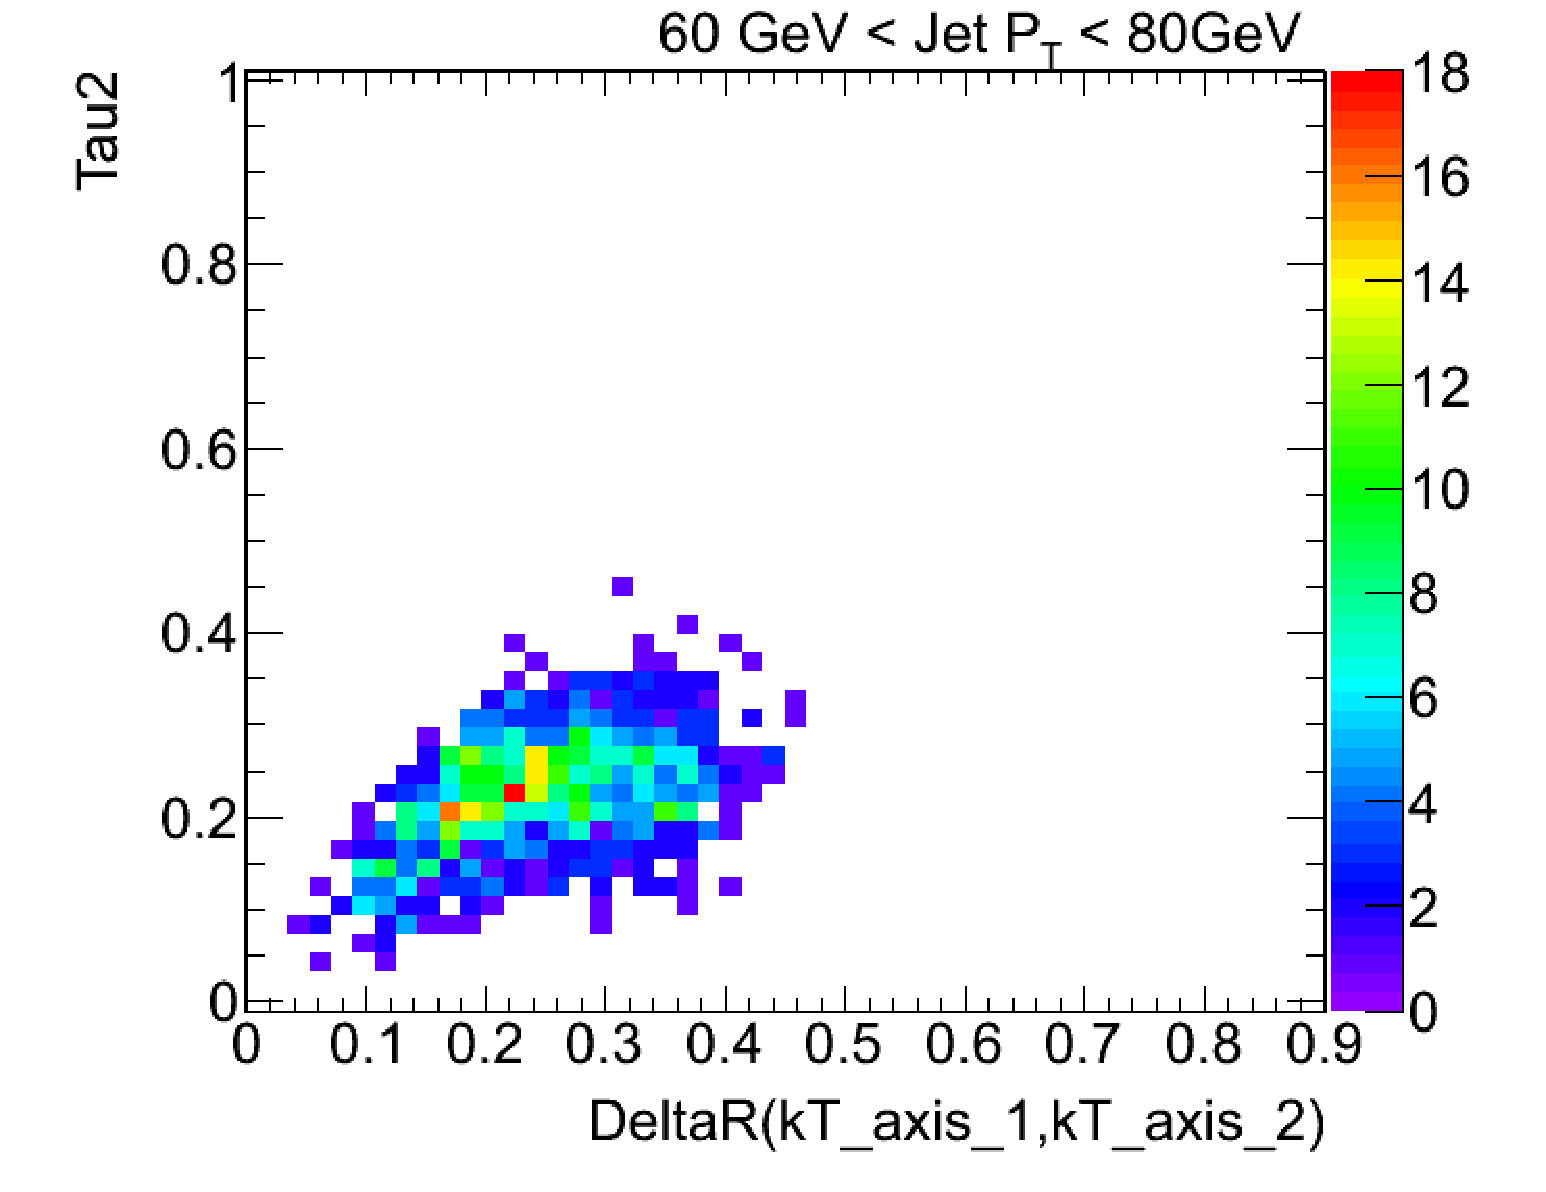
\includegraphics[width=0.49\textwidth]{FIGS/TEMPFigs/PythisStandalone/Antikt4/allparticles/Tau2DRkT2axesCorr_PT60_merged.pdf}
\caption{Correlation between $\tau_1$ (left) and $\tau_2$ (right) and the $\Delta R$ between the $k_T$ subjets in merged anti-$k_T$ 0.4 jets  between 60~GeV to 80~GeV. Jets were built using all stable particles.}
\label{fig:CorrTau1Tau2DRkt}
\end{figure}

%See email from Jesse Thaler
%Thu, Jun 2, 2011 at 7:43 PM
%subject:	 Re: N-subjettiness Code
%This is really fascinating, and it is starting to make some physical sense.  
For the single $b$-jets, $\tau_1$, $\tau_2$, and $\Delta R$ between the $k_T$ axes in the jet are all small which is expected for a pencil-like jet.  For the $b \bar{b}$-jets, these variables are all large, which is typical of a gluon jet.  But the correlations are really fascinating in merged $b$-jets.   $\tau_1$ and $\Delta R$ between the $k_T$ axes are nearly linearly related, which is expected if there are two hard lobes of energy.  But $\tau_2$ is almost independent of $\Delta R$ between the $k_T$ axes, meaning that regardless of where the axes are, the energy is uniformly distributed around them.
%So the question is whether you can make use of this.  tau1 and deltaR_12 are clearly useful variables, but they are also quite correlated.  tau2 appear to be uncorrelated with deltaR_12, but semi-correlated with tau_1.  By eye, the best discriminator for the R = 0.4 jets looks to be something like
%tau2 > (10 GeV/pT), deltaR_12 > (10 GeV/pT)
%or maybe
%(tau2 + deltaR_12) >  (20 GeV/pT).
%At this point, what would be helpful is to know whether your selection is really picking out g>bb jets or just picking up gluon jets in general.  For example, is the tau2 vs deltaR_12 non-correlation the same for generic gluon jets, or is it special to g>bb?  My intuition is that this must be a special feature of g>bb, since otherwise, it would be quite easy to separate gluon jets from quark jets...


%See this page for comparisons between g/b/bb from Max
%http://slac.stanford.edu/~swiatlow/gbb_plots/plots.html

%See mail from ariel 2 Jun 2011
%Quiza lo que este ocurriendo es que gbb fragmenta como normal (gluon) qcd, con mas splittings que b-jets (quarks) y sin la 2-body decay structura que estamos esperando.

%Date: Thu, 2 Jun 2011 20:37:57 +0200
%From: Ariel Schwartzman <sch@slac.stanford.edu>
%To: Maria Laura Gonzalez Silva <laugs@mail.cern.ch>
%Cc: Ricardo Piegaia <aia@df.uba.ar>, Laura <laugs@cern.ch>
%Subject: Re: N-subjettiness
% Muy interesante Laura.
% Tau1 aumenta con DRbb, como se espera, pues es como el jet width.
% Tau2 es casi flat con DR, lo que puede indicar dos cosas:
%  i) los kt-axis a los que se refiere Jesse no estan encontrando los dos B's
% ii) la contribucion de los tracks from B's es pequenia comparada con el resto de la fragmentacion, de modo de a que un gbb jet seria ungluon jet plus algunos soft displaced tracks on top.
% Te propngo algunos plots:
% 1) Jesse sugiere plotar el DR entre los dos kt axes para b y bb. Espero que quede claro en su codigo como axeder a esta variable...
% 2) Hace un 2D plot con la correlacion entre el DR entre los axes (1) y DR(B,B) para ver si esta definicion de axes corresponde a lo queesperamos.
%3) Vos habias mirado a DR(1,2) que es el DR entre los dos leading tracks. Podrias re-vivir estos estudios ahora con el generator study? Yhacer tambien el 2D plot de DR(1,2) vs DR(B,B)?
%4) Seria bueno repetir todas las input variables para pure gluon jets (esto lo sugeri en un mail el otro dia) para entender mejor cual es la diferencia entre gluones y gbb.
%5) Los dos blobs de energy que esperamos vienen de la hadronizacion de los B hadrons, mas que de la fragmentacion del gluon. Quiza estesea un key point que estamos ignorando. Yo estoy tentado a sugerir que calculemos las variables usando "displaced tracks" solamente. Ricardo, es posible ponerle un flag a las particulas que vienen de los B decays como para que Laura solo use estas particulas para calcular N-subjettiness?
%6) Event displays... son como la tool ideal para entender que esta pasando. Uno puede mirar event displays para jets con distinto DR(B,B), distuntos taus, etc... Fijate que todavia no tenemos una picture de cual es la shape de un gbb jet! Estuvimos asumiendo que uno espera 2 blobs de energy, pero no tenemos ningun plot que soporte esta idea en forma contundente.
%En todo caso, me parace perfecto tener esta discucion con Jesse. Ciertamente vamos a aprender mucho mas sobre gluon splitting...




%------------------------------------------------------------------------
\section{Kinematid differences between single $b$- and merged $b\bar{b}$-jets}\label{sec:gbbKine}
%\section{Full ATLAS Monte Carlo Analysis}\label{sec:gbbKine}
%------------------------------------------------------------------------ 



The differences between genuine $b$-quark jets and $b \bar{b}$ jets are expected to arise from the two-subjet (two $B$-hadrons) substructure of merged jets.  They are thus expected, for the same jet $\pt$, to have higher track-multiplicity and be wider than single $b$-jets. Based on these characteristics %, the following properties were studied in simulated QCD samples of $b$-tagged jets using either calorimeter or track constituents:
simulated QCD samples of $b$-tagged jets were used to study the following properties, discussed in the next paragraphs, built from jet constituents either at calorimeter level (topological clusters) or tracks associated to the jet:

\begin{itemize}\addtolength{\itemsep}{-0.4\baselineskip}
\item
Jet multiplicity (number of constituents)
\item
Jet width, $\pt$ weighted %Track jet width ($\pt$ weighted)
\item 
Jet Mass
\item
Nr.\ of $k_t$ subjets %track-jets
\item
Maximum $\Delta R$ between pairs of constituents % (tracks)
\item
$\Delta R$ between 2 $k_t$ subjets within the $b$-jet
\item
$\tau_2$: 2-subjettiness 
\item
$\tau_2/\tau_1$
\item
$\Delta R$ of leading constituents %tracks
\item 
Eccentricity %(track & calo)
\end{itemize}


%Figures~\ref{fig:ntrksinglemerged} to~\ref{fig:tauratiosinglemerged} show the distributions and correlations of some of these variables in selected bins of $b$-tagged jet $\pt$. 

{ \em I. Jet track multiplicity}
\\[3mm]
This variable is defined as the number of tracks associated to the jet, it is simple to calculate and carries important information of the jet inner structure. Figure~\ref{fig:ntrksinglemerged} shows the distribution of the observable for single and merged $b$-jets.  It was observed that merged $b$-jets contain on average around two more tracks than single $b$-jets at low jet $\pt$, with a larger difference at higher $\pt$ values. The jet track multiplicity corresponds to tracks with $\pt$ above 1 GeV, satisfying the quality cuts described in section~\ref{sec:EventSelection}. The effect of using a minimum track $\pt$ of 0.5 GeV was also examined. This was motivated by the fact that it could lead to an improvement in discrimination if it captured more information about the fragmentation process.  On ther other hand, a lower minimum track $\pt$ can make the method more sensitive to pile-up with the addition of soft tracks incorrectly associated to the jets.  What it was observed is that reducing the $\pt$ cut only widens the distributions without increasing the separation between single and merged jets. 
\begin{figure}[tp]
\centering
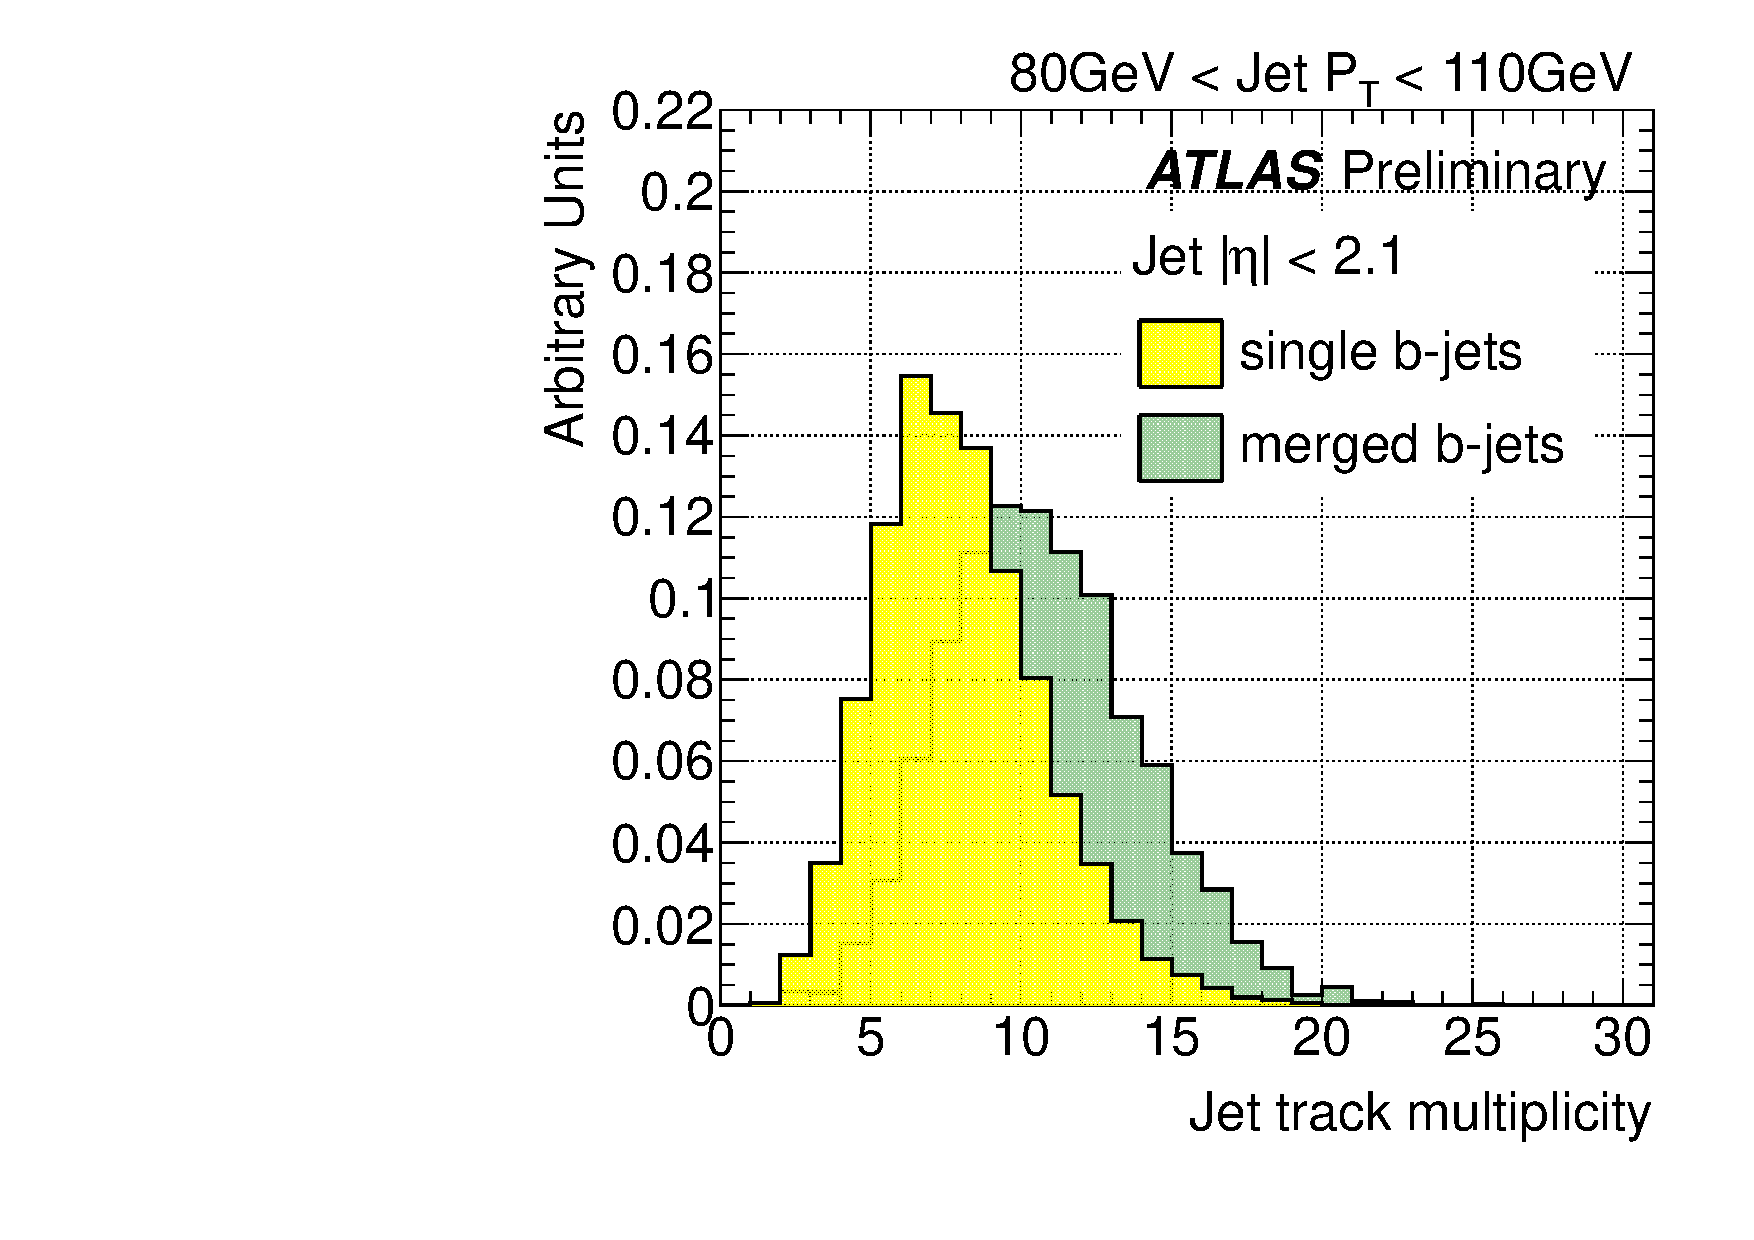
\includegraphics[width=0.49\textwidth]{FIGS/VarsSingleMerged/Ntrk080.pdf}
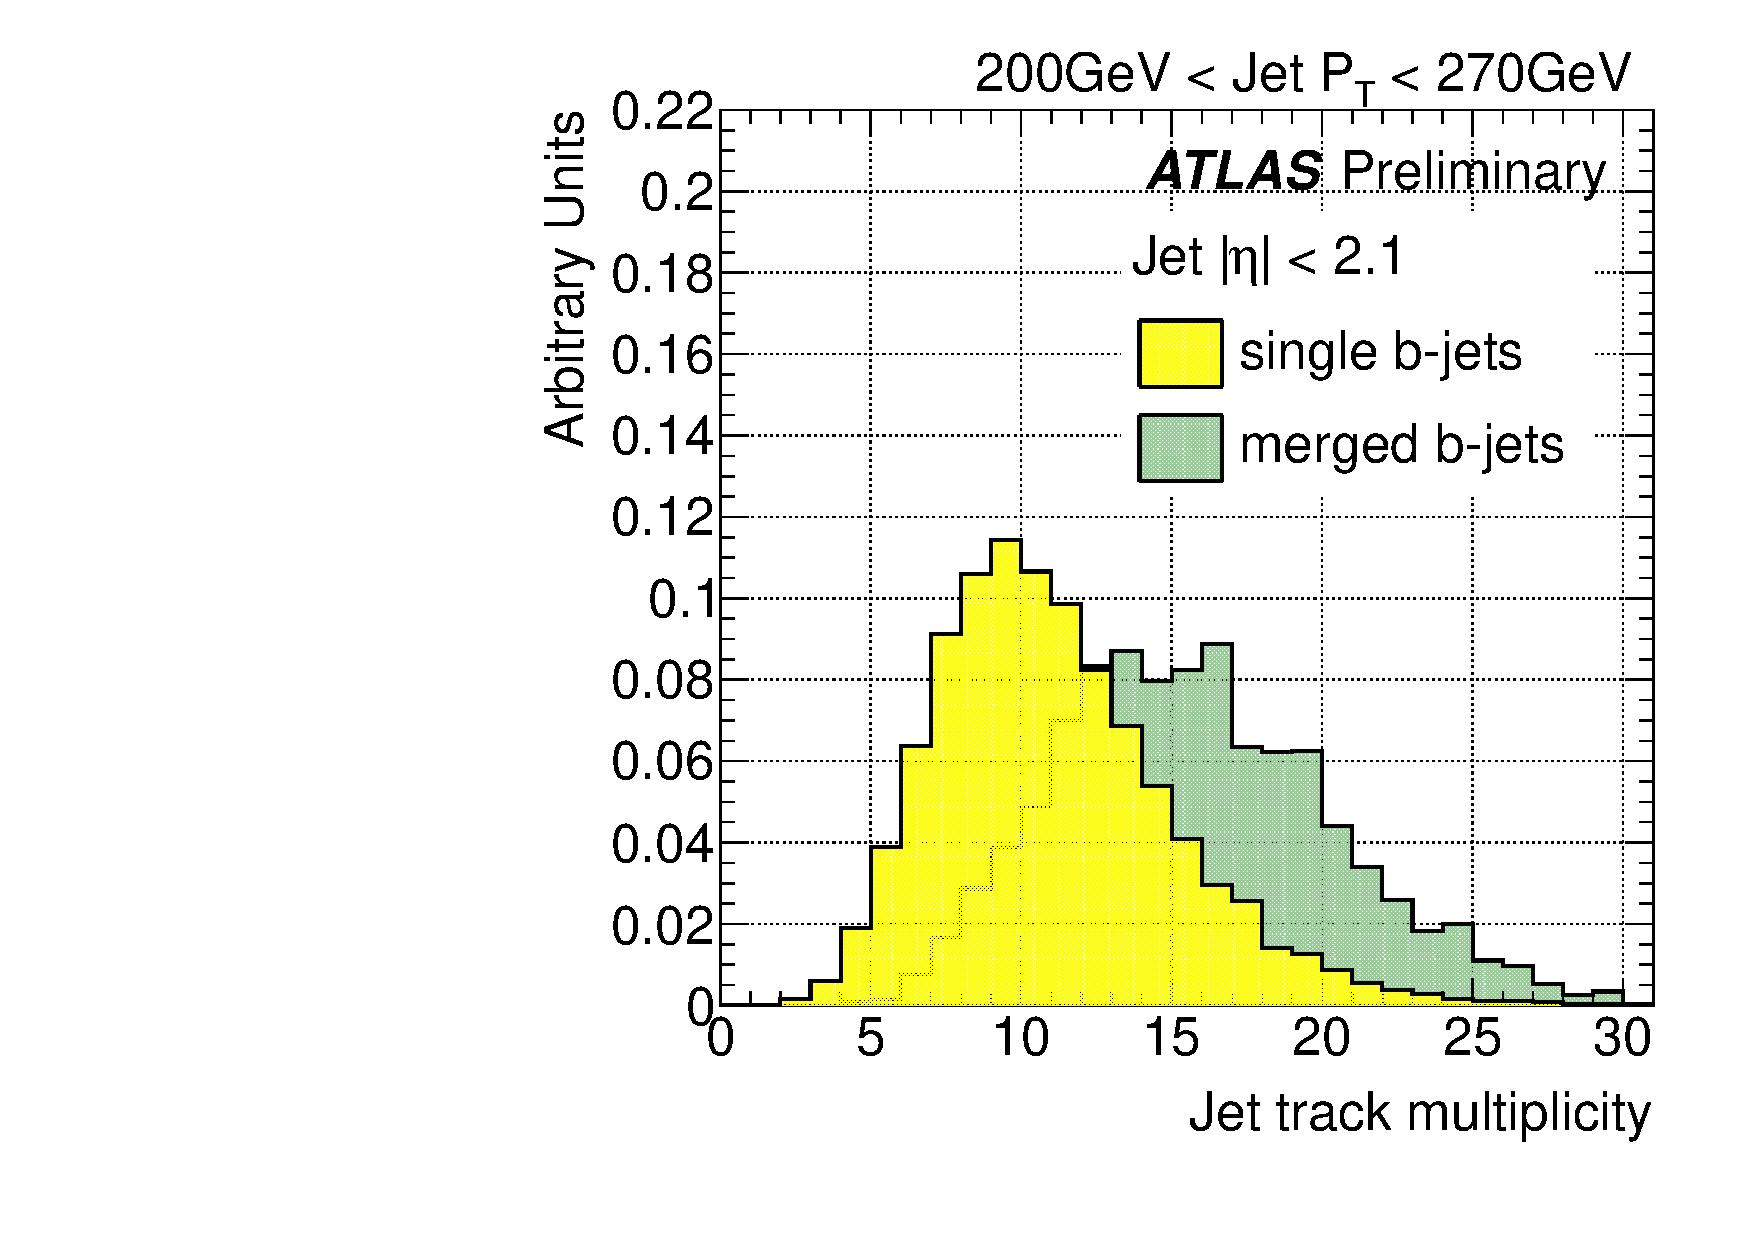
\includegraphics[width=0.49\textwidth]{FIGS/VarsSingleMerged/Ntrk200.pdf}
\caption{Distribution of the track multiplicity in jets for single and merged $b$-jets between 80~GeV to 110~GeV (left) and 200~GeV to 270~GeV (right).}
\label{fig:ntrksinglemerged}
\end{figure}

{ \em II. Jet width}
\\[3mm]
 The jet width was computed as the $\pt$ weighted average of the $\Delta R$ distance between the associated constituent (``$const$'') and the jet axis:
\begin{equation} 
\mbox{ {\it Jet width}} = \frac{\sum_{i=1}^N \pt^{const_i} \,\Delta R (const_i,jet) }{\sum_{i=1}^N \pt^{const_i} }
\label{eqn:trackjetwidth}
\end{equation} 
where $N$ is the total number of calorimeter or track constituents.

Figure~\ref{fig:trkwidthsinglemerged} shows the distribution for the Track-jet width. As expected, merged $b$-jets are wider than single $b$-jets. In Fig.~\ref{fig:ntrktrkwidthsinglemerged} the correlation between the track-jet width and the jet track multiplicity is shown for single and merged $b$-jets. These two variables alone provide a good discrimination for tagging $b \bar{b}$ jets.

The calorimeter jet width ( using topological clusters) gives also good separation. However, this variable is more sensitive to the amount of pile-up in the event than its track-based counterpart. In Fig.~\ref{fig:calowidthpileup} the distributions of calorimeter width for single and merged $b$-jets  can be seen for events with low and high Number of Primary Vertices (NPV), in a low $\pt$ region where the effect of pile-up is more important. In Fig.~\ref{fig:trkwidthpileup} the same distributions are shown for the track-jet width. Calorimeter jet width varies %significatively
with NPV and due to this behavior the track-based version is more suitable as a more robust discriminator. For similar reasons, the jet topological cluster multiplicity and the jet mass were discarded as discriminating variables.
\\[3mm]

\begin{figure}[tp]
\centering
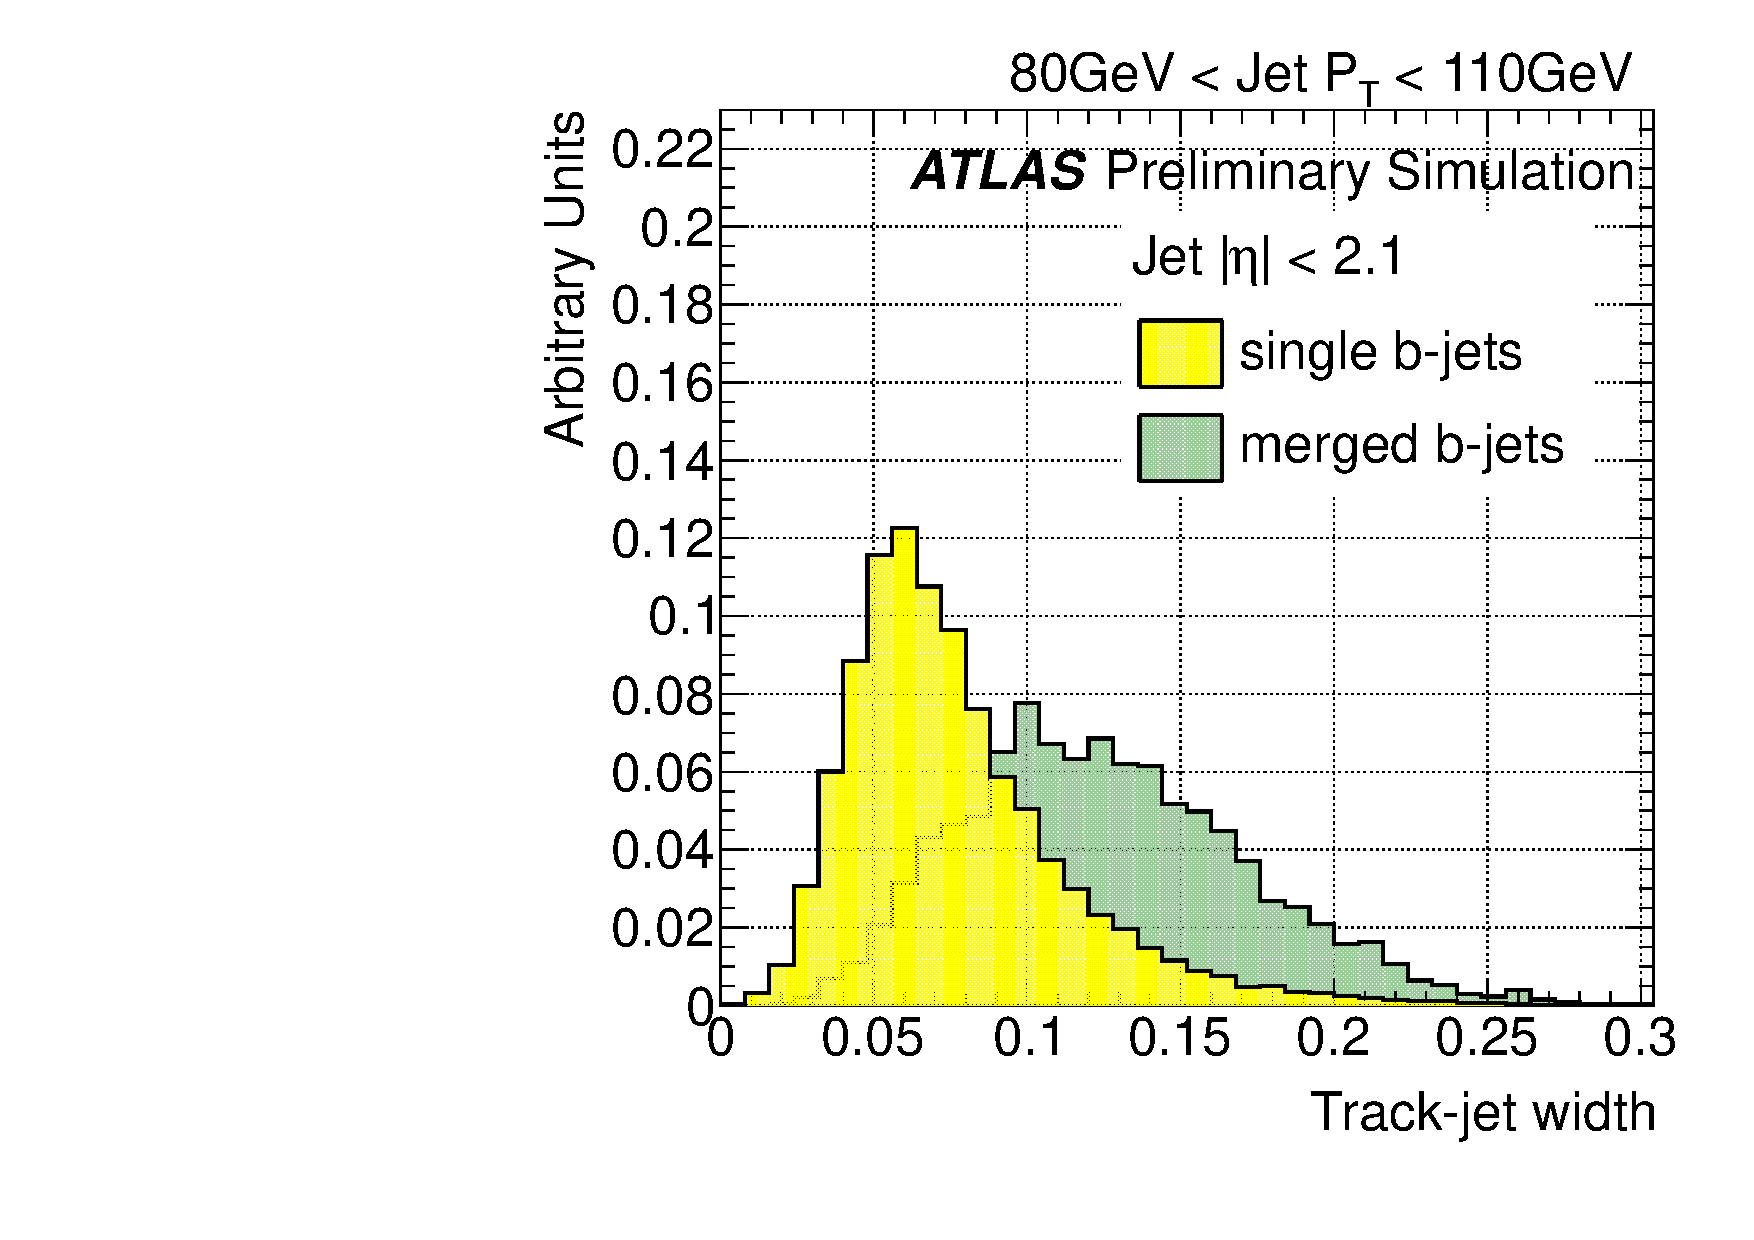
\includegraphics[width=0.49\textwidth]{FIGS/VarsSingleMerged/trkWidth080.pdf}
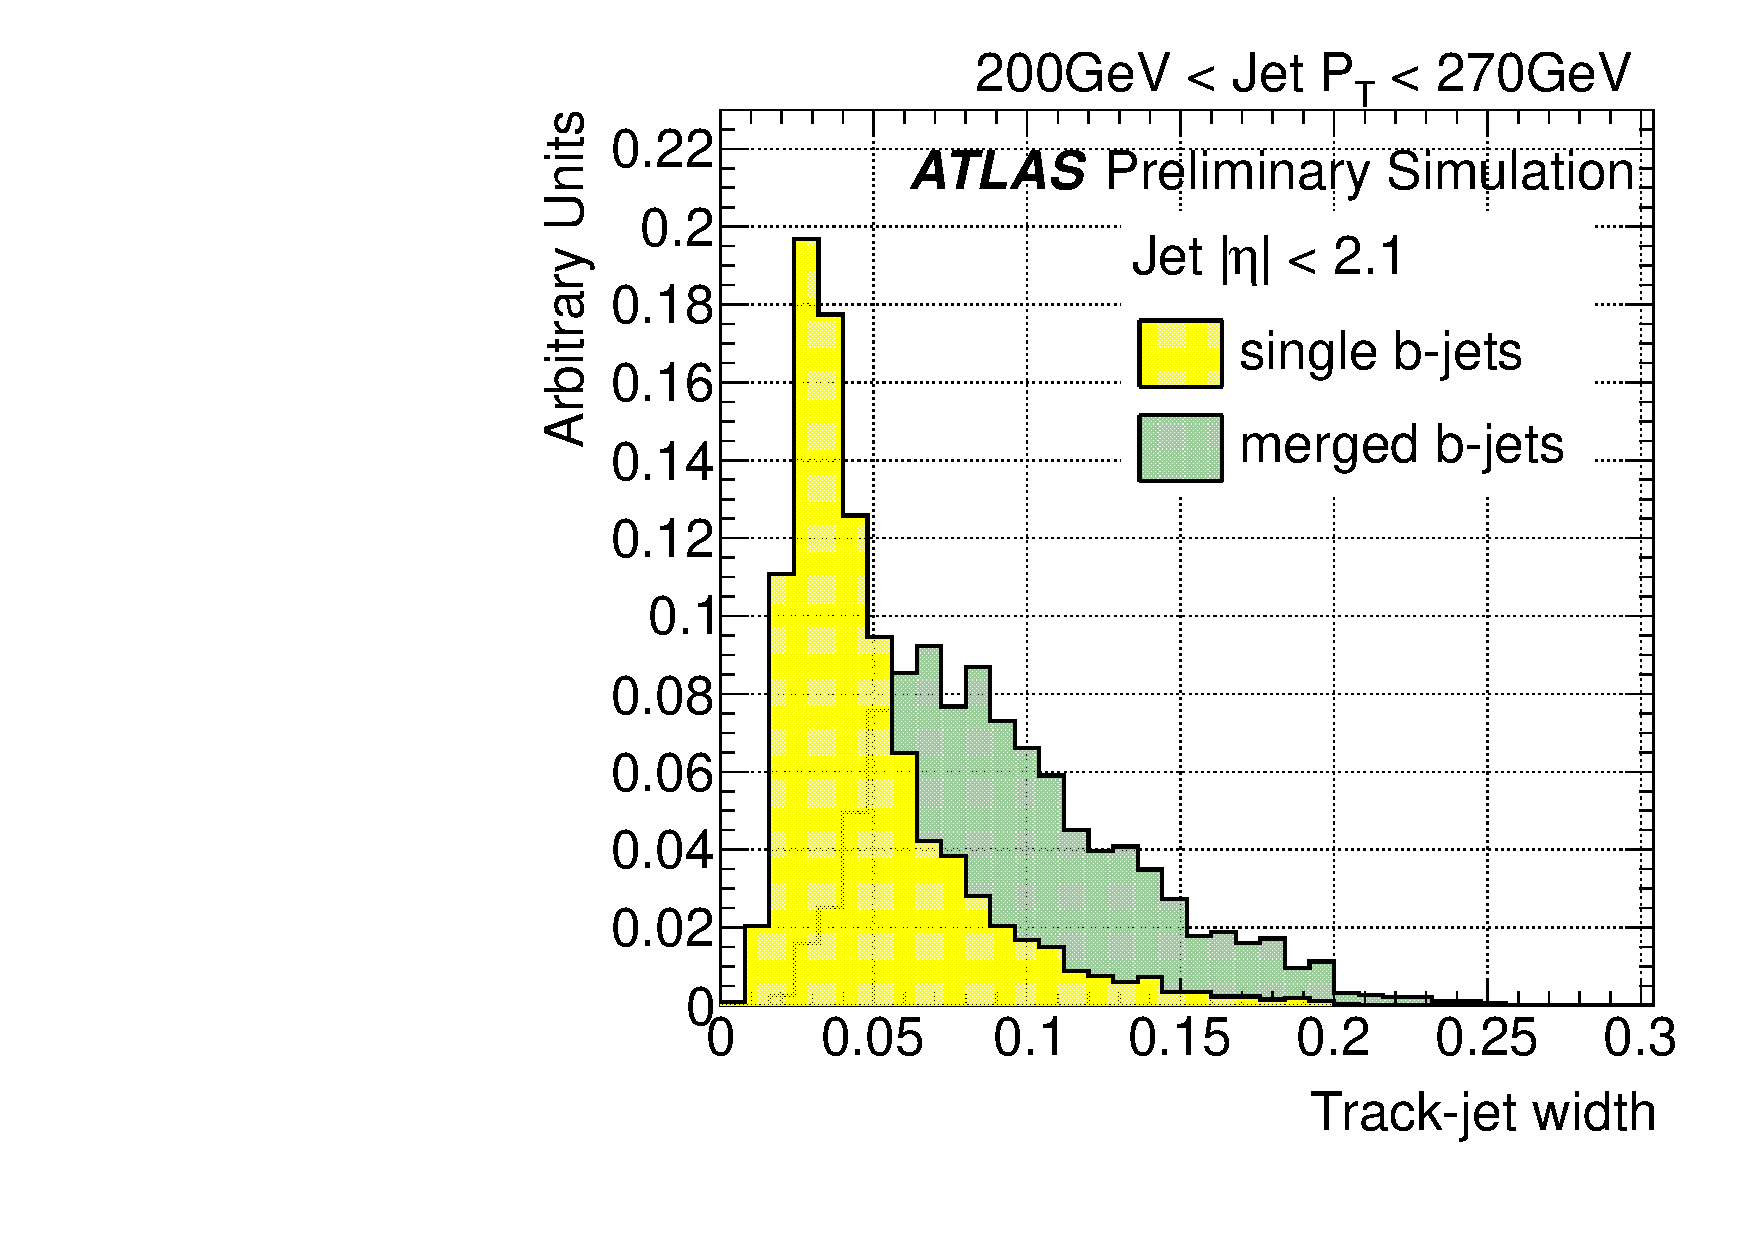
\includegraphics[width=0.49\textwidth]{FIGS/VarsSingleMerged/trkWidth200.pdf}
\caption{Distribution of track-jet width in jets for single and merged $b$-jets between 80~GeV to 110~GeV (left) and 200~GeV to 270~GeV (right).}
\label{fig:trkwidthsinglemerged}
\end{figure}

\begin{figure}[tp]
\centering
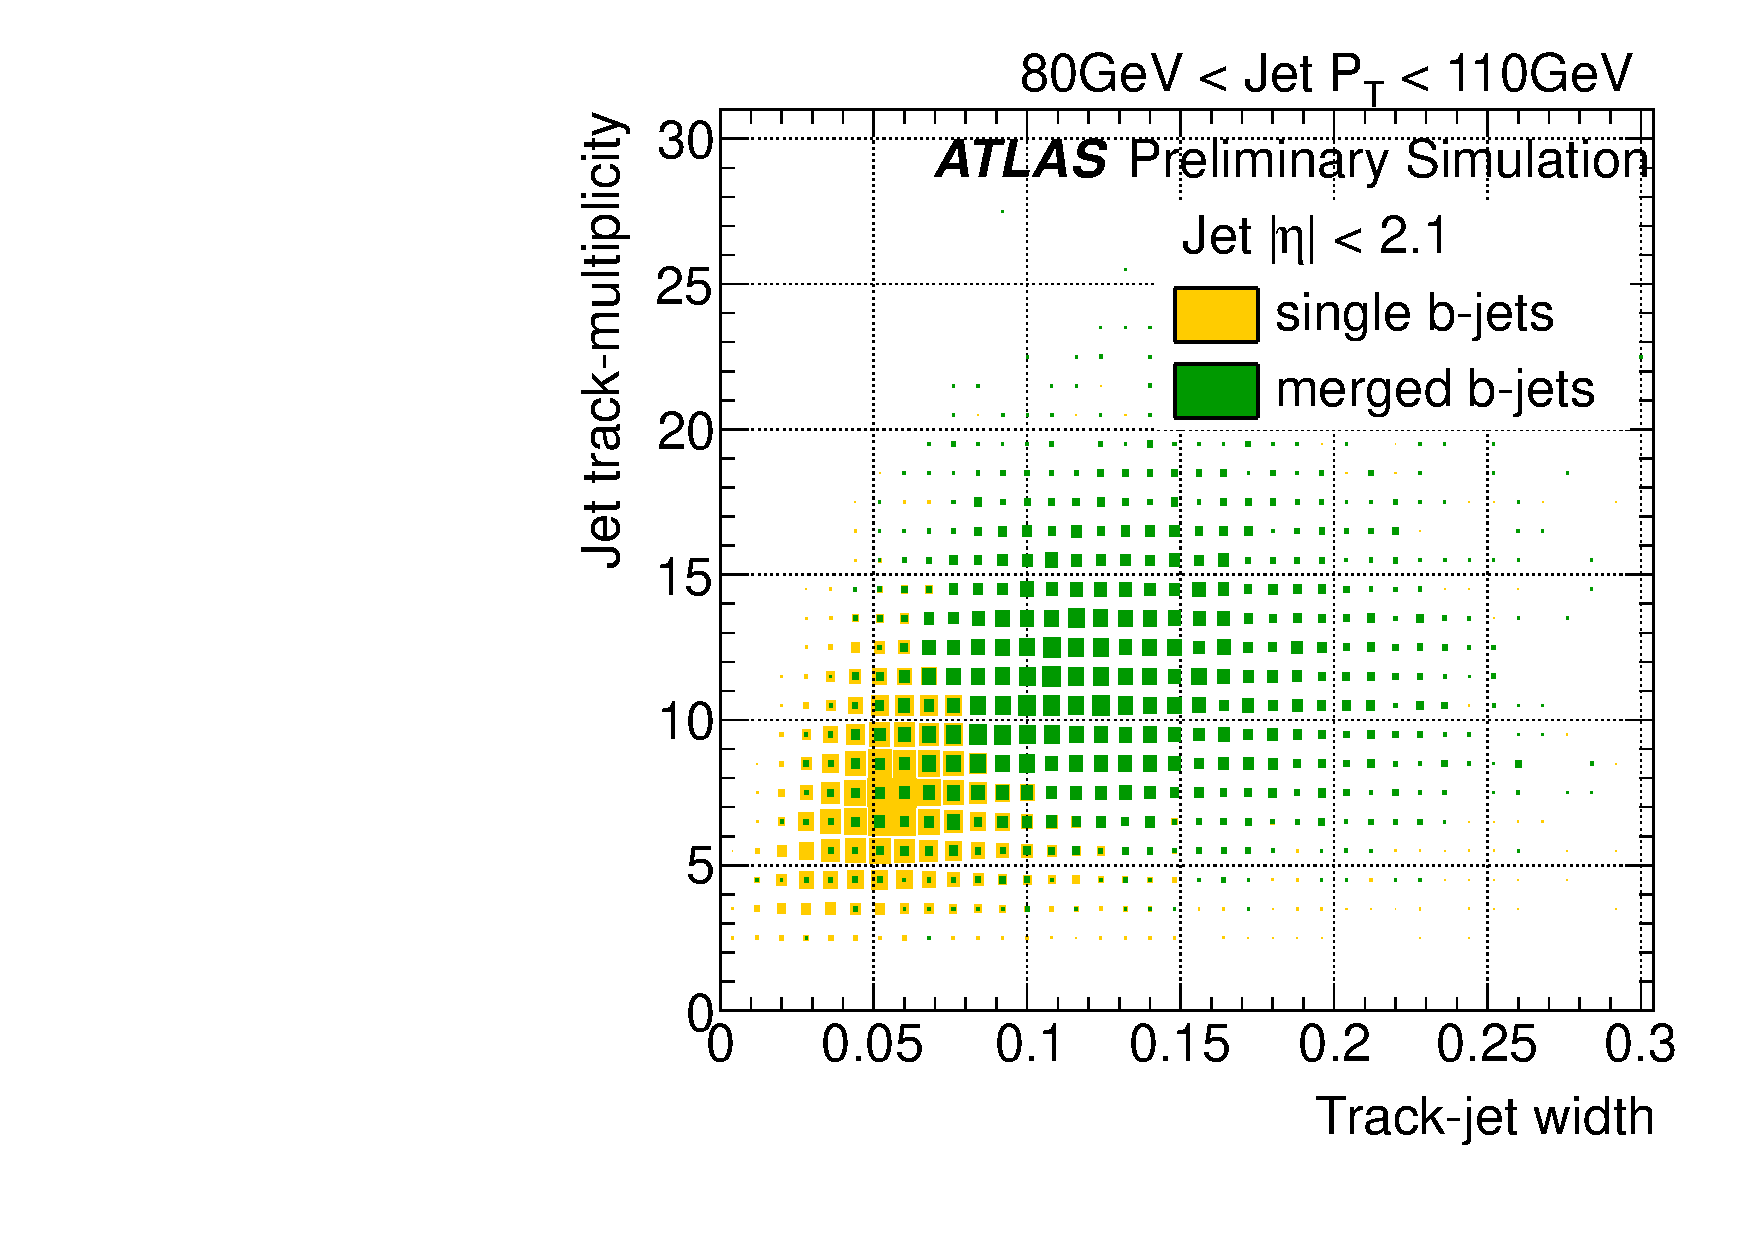
\includegraphics[width=0.49\textwidth]{FIGS/VarsSingleMerged/NtrktrkWidth080.pdf}
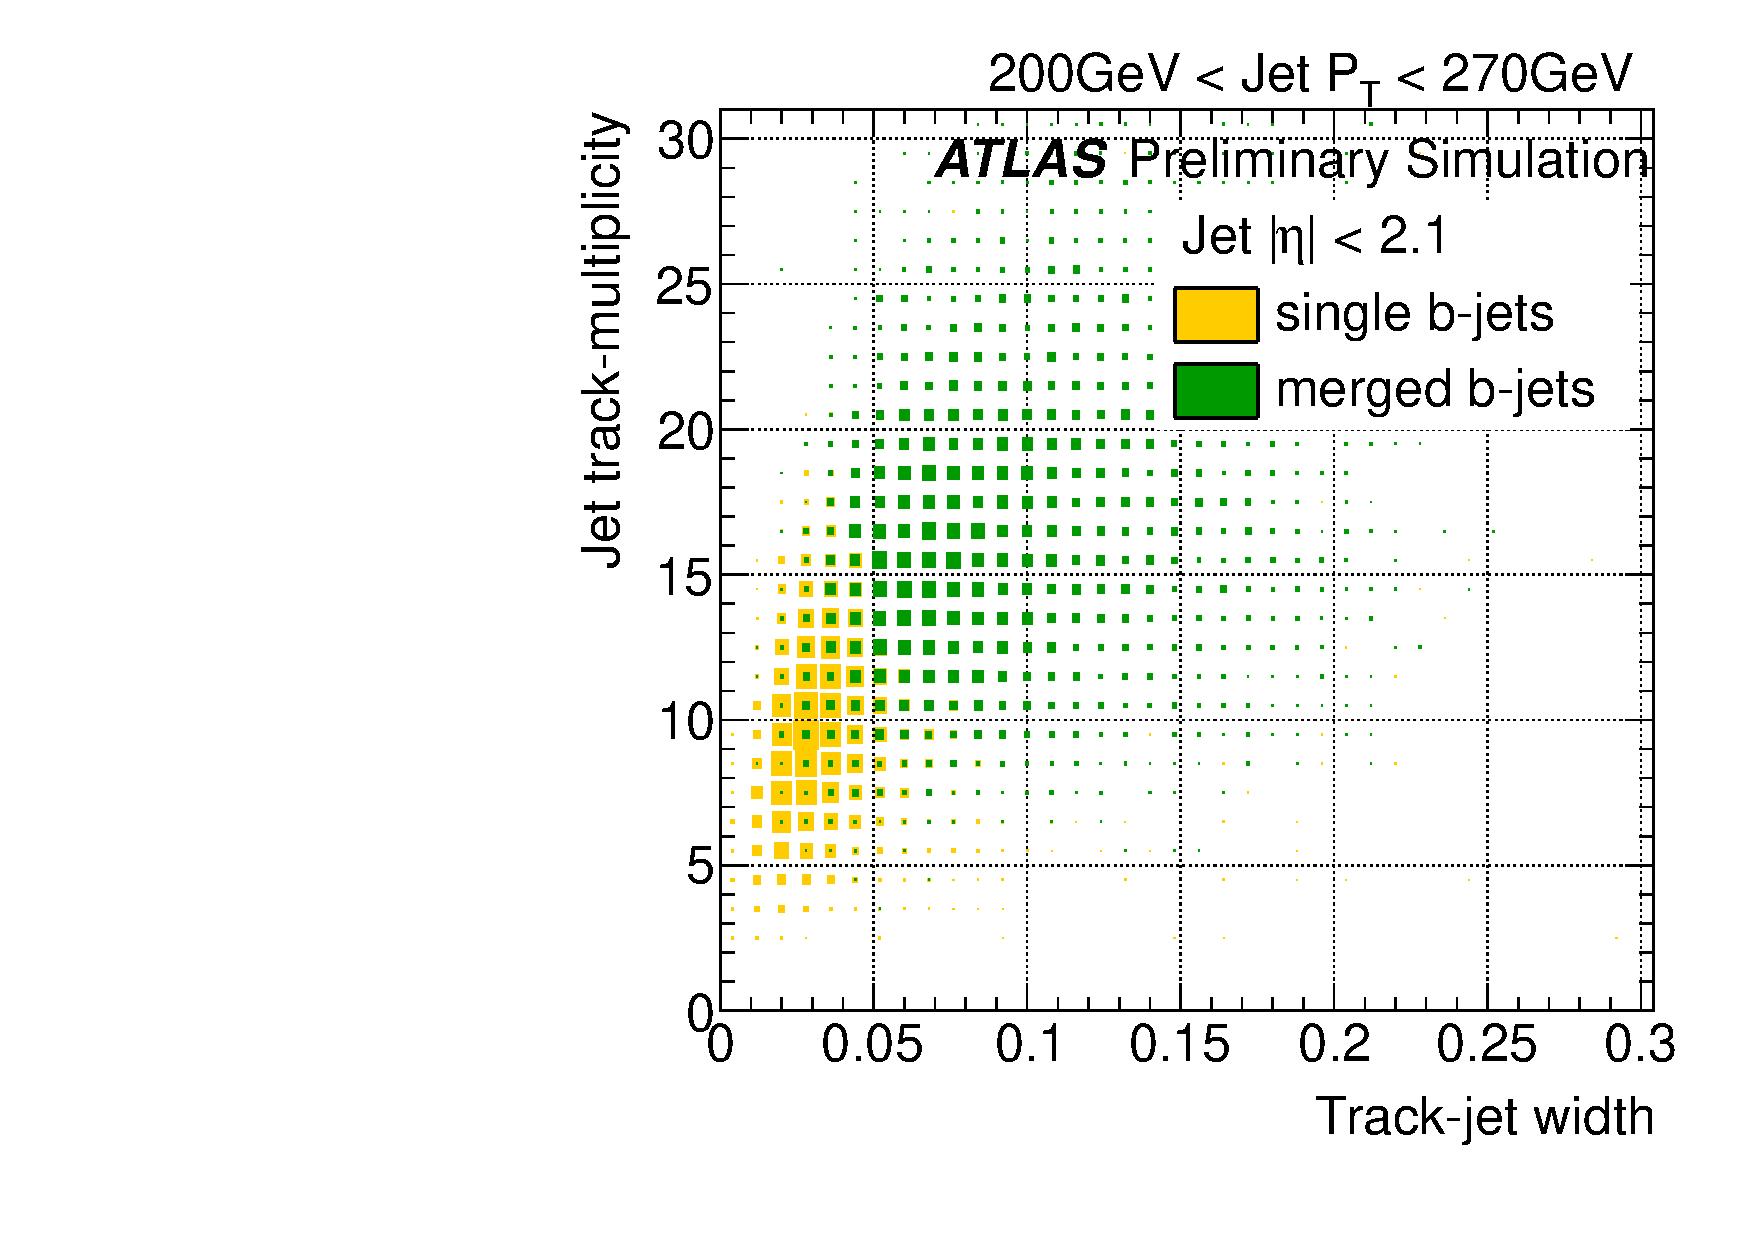
\includegraphics[width=0.49\textwidth]{FIGS/VarsSingleMerged/NtrktrkWidth200.pdf}
\caption{Correlation between jet track multiplicity and track-jet width for single and merged $b$-jets between 80~GeV to 110~GeV (left) and 200~GeV to 270~GeV (right).}
\label{fig:ntrktrkwidthsinglemerged}
\end{figure}

\begin{figure}[tp]
\centering
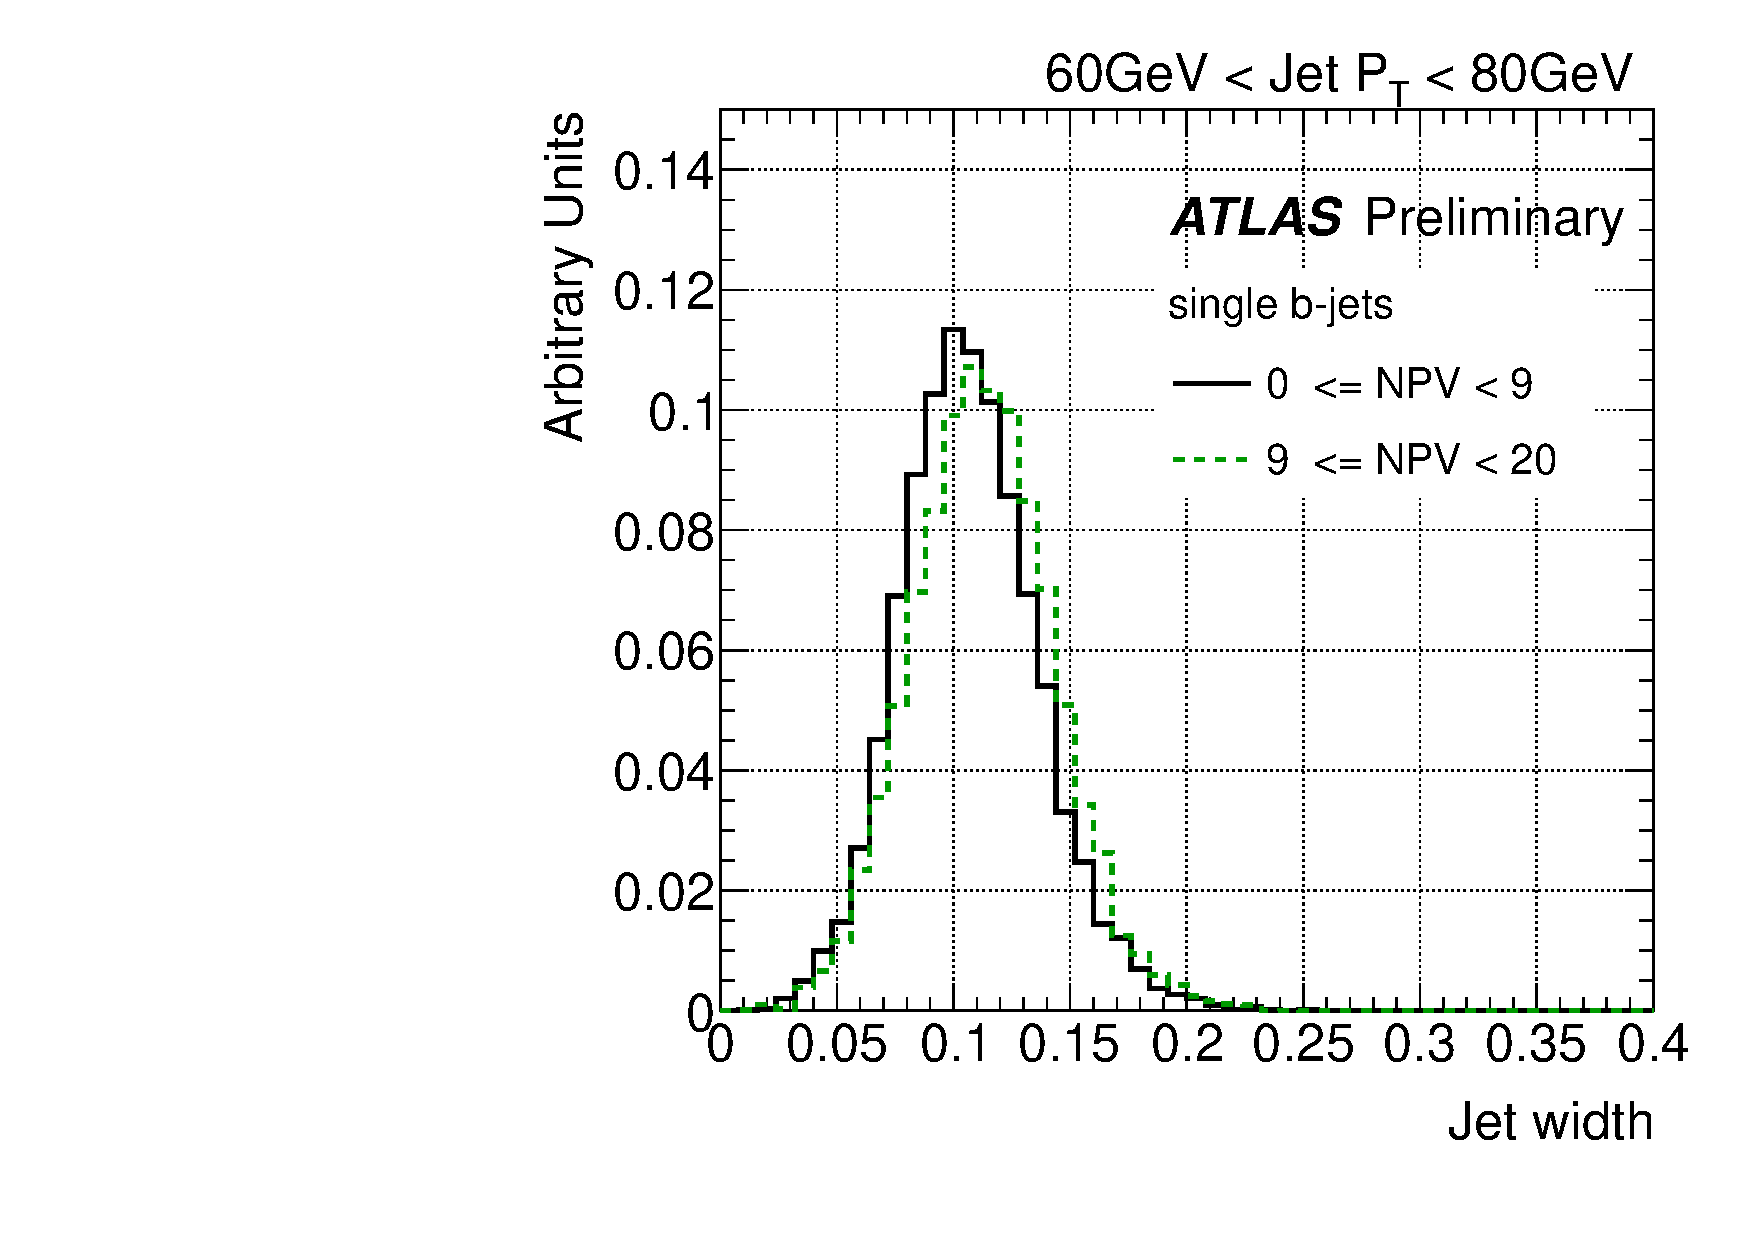
\includegraphics[width=0.49\textwidth]{FIGS/systematics/Widthsingle_060.pdf}
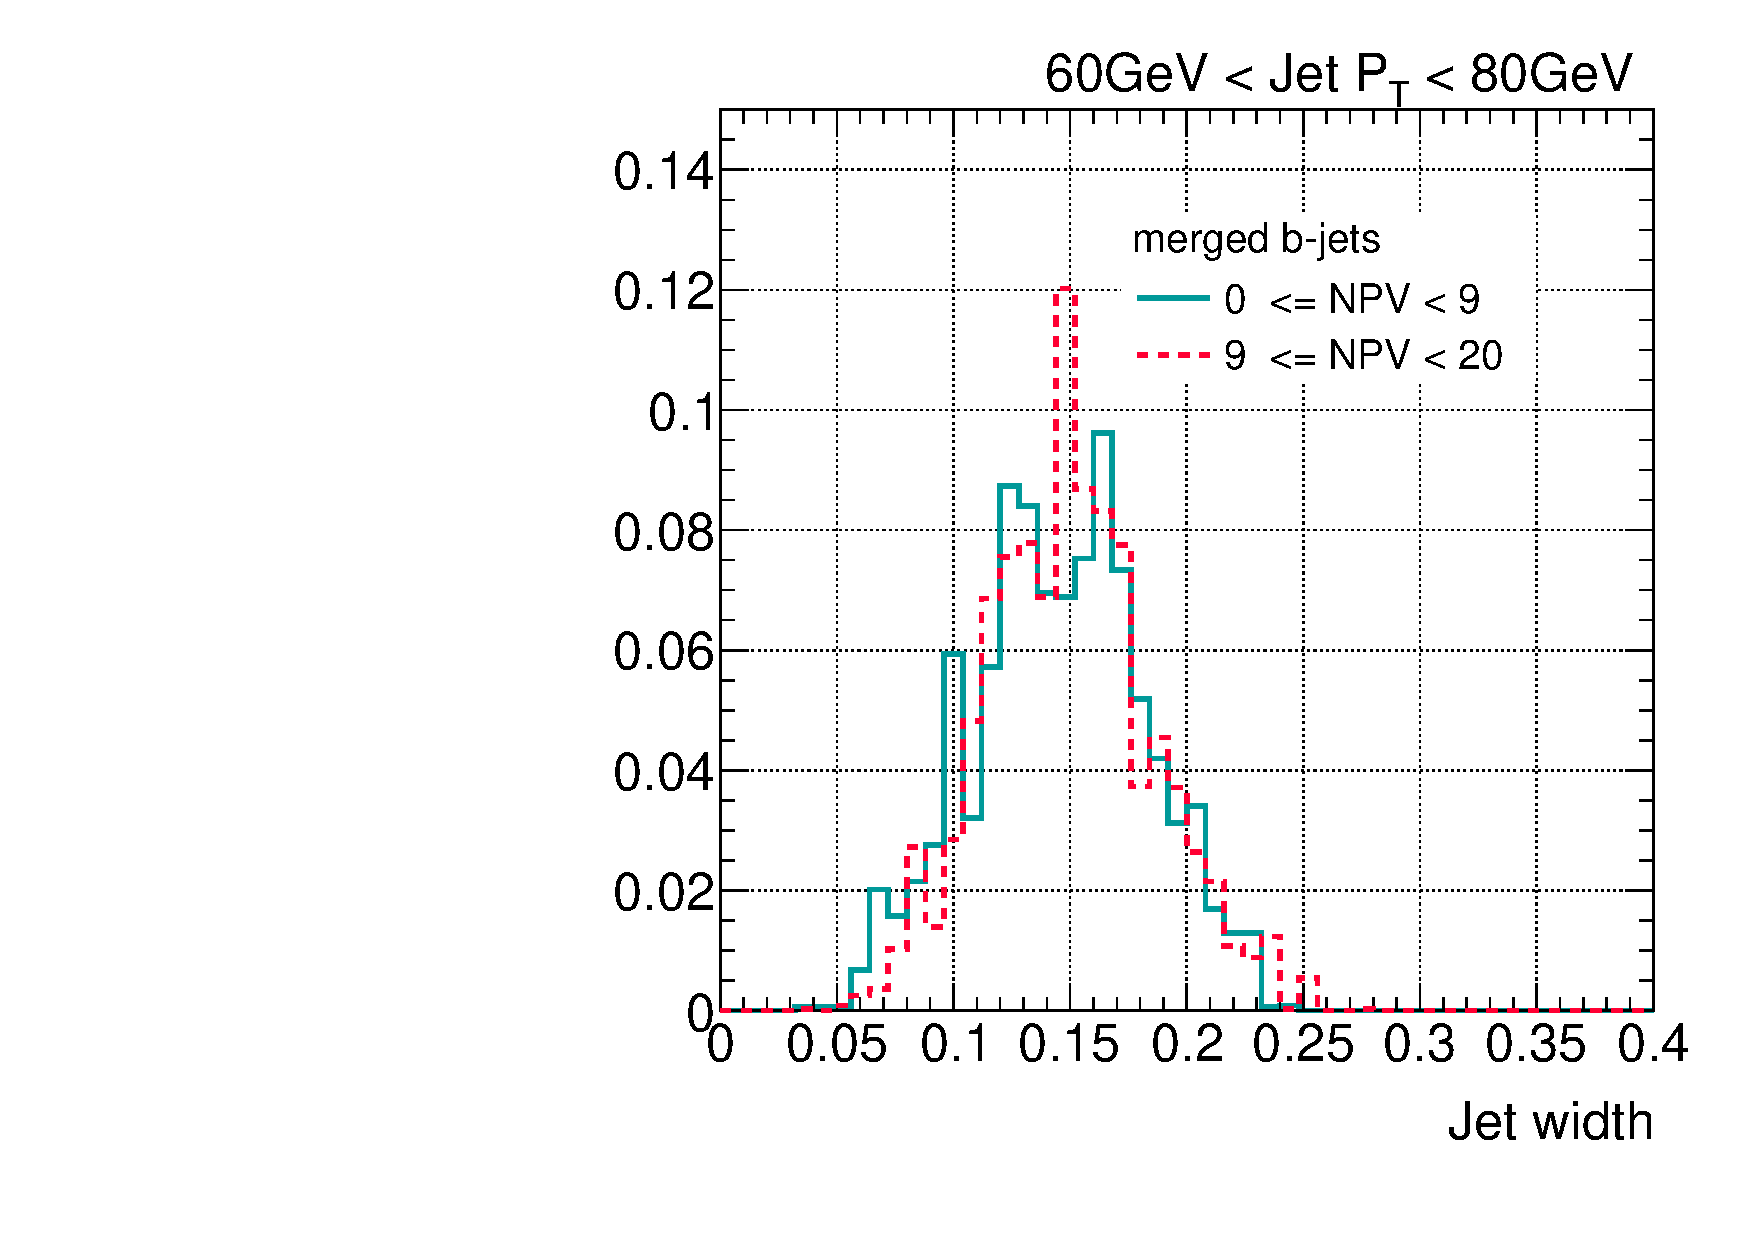
\includegraphics[width=0.49\textwidth]{FIGS/systematics/Widthmerged_060.pdf}
\caption{Distribution of calorimeter jet width (using topological clusters) for single (left) and merged (right) $b$-jets in two bins of Number of Primary Vertices for jets between 60~GeV to 80~GeV.}
\label{fig:calowidthpileup}
\end{figure}


\begin{figure}[tp]
\centering
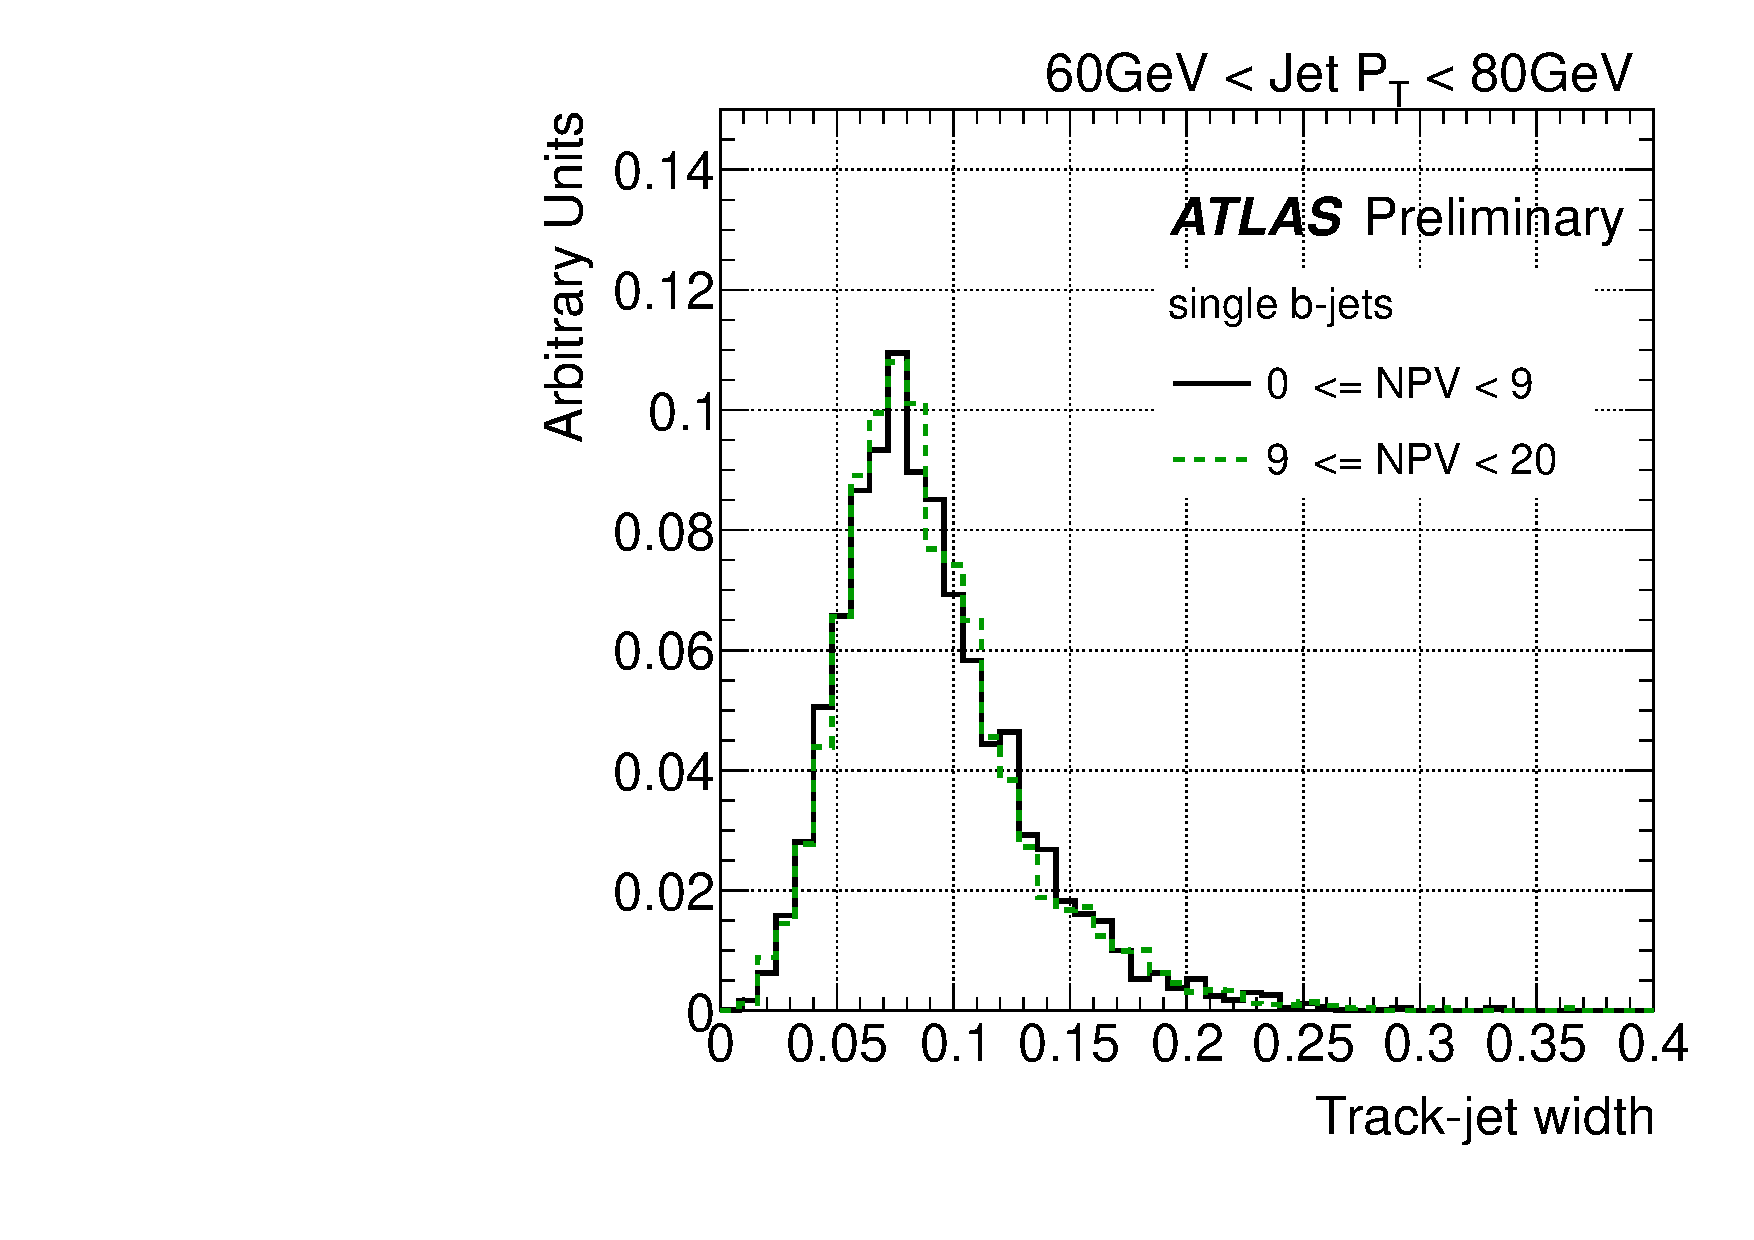
\includegraphics[width=0.49\textwidth]{FIGS/systematics/trkWidthsingle_060.pdf}
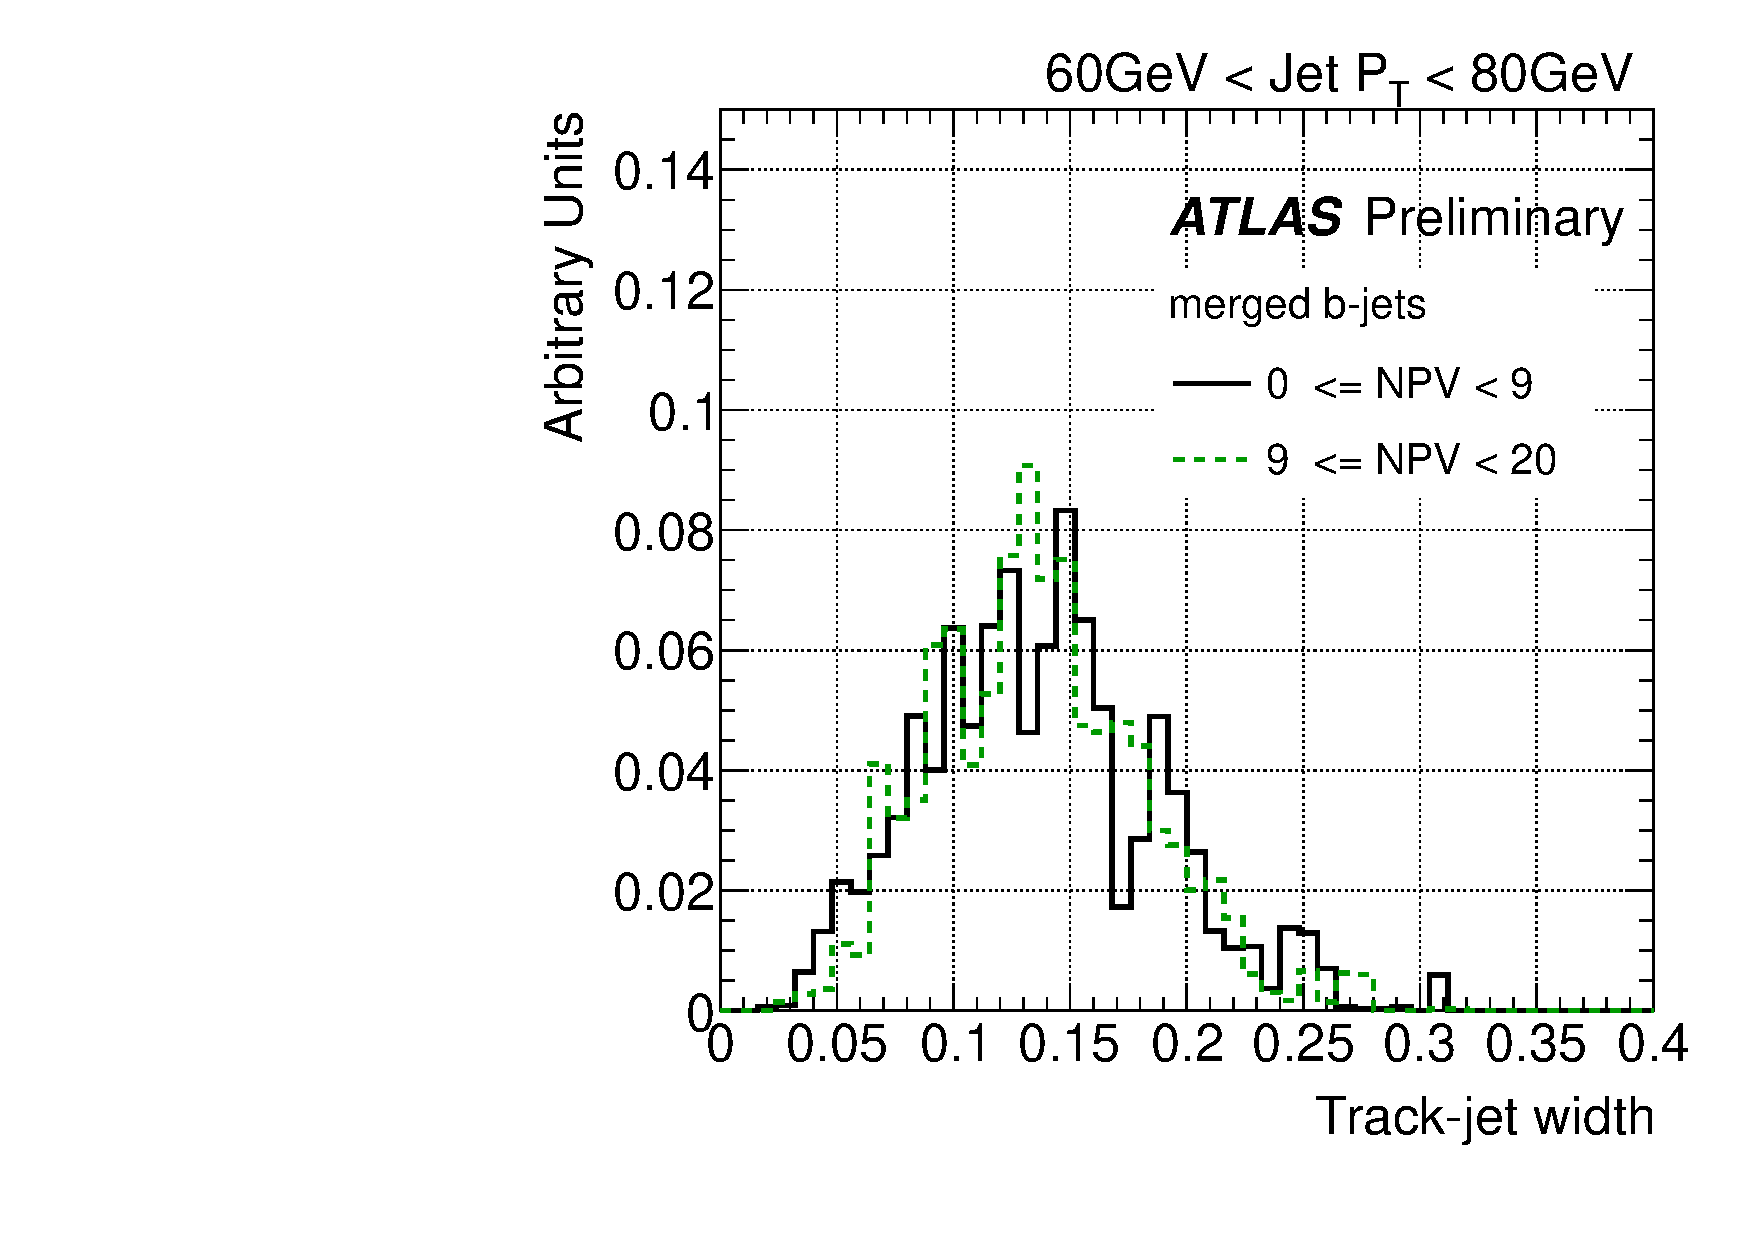
\includegraphics[width=0.49\textwidth]{FIGS/systematics/trkWidthmerged_060.pdf}
\caption{Distribution of track-jet width for single (left) and merged (right) $b$-jets in two bins of Number of Primary Vertices for jets between 60~GeV to 80~GeV.}
\label{fig:trkwidthpileup}
\end{figure}



{ \em III. Maximum $\Delta R$ between track pairs}
\\[3mm]
Figure~\ref{fig:drmaxsinglemerged} shows the distribution of the maximum $\Delta R$ between track pairs in the jets (Max$\{\Delta R(trk,trk)\}$). Merged $b$-jets show significantly higher values for this variable over a broad range of jet $\pt$. The distinct characteristic of this variable is that the separation between single $b$-jets and merged does not depend on jet $\pt$. In spite of its good discrimination power, we have looked for alternatives to Max$\{\Delta R(trk,trk)\}$ as it is not an infrared safe observable and is sensitive to soft tracks originating from pile-up. 
\\[3mm]

\begin{figure}[tp]
\centering
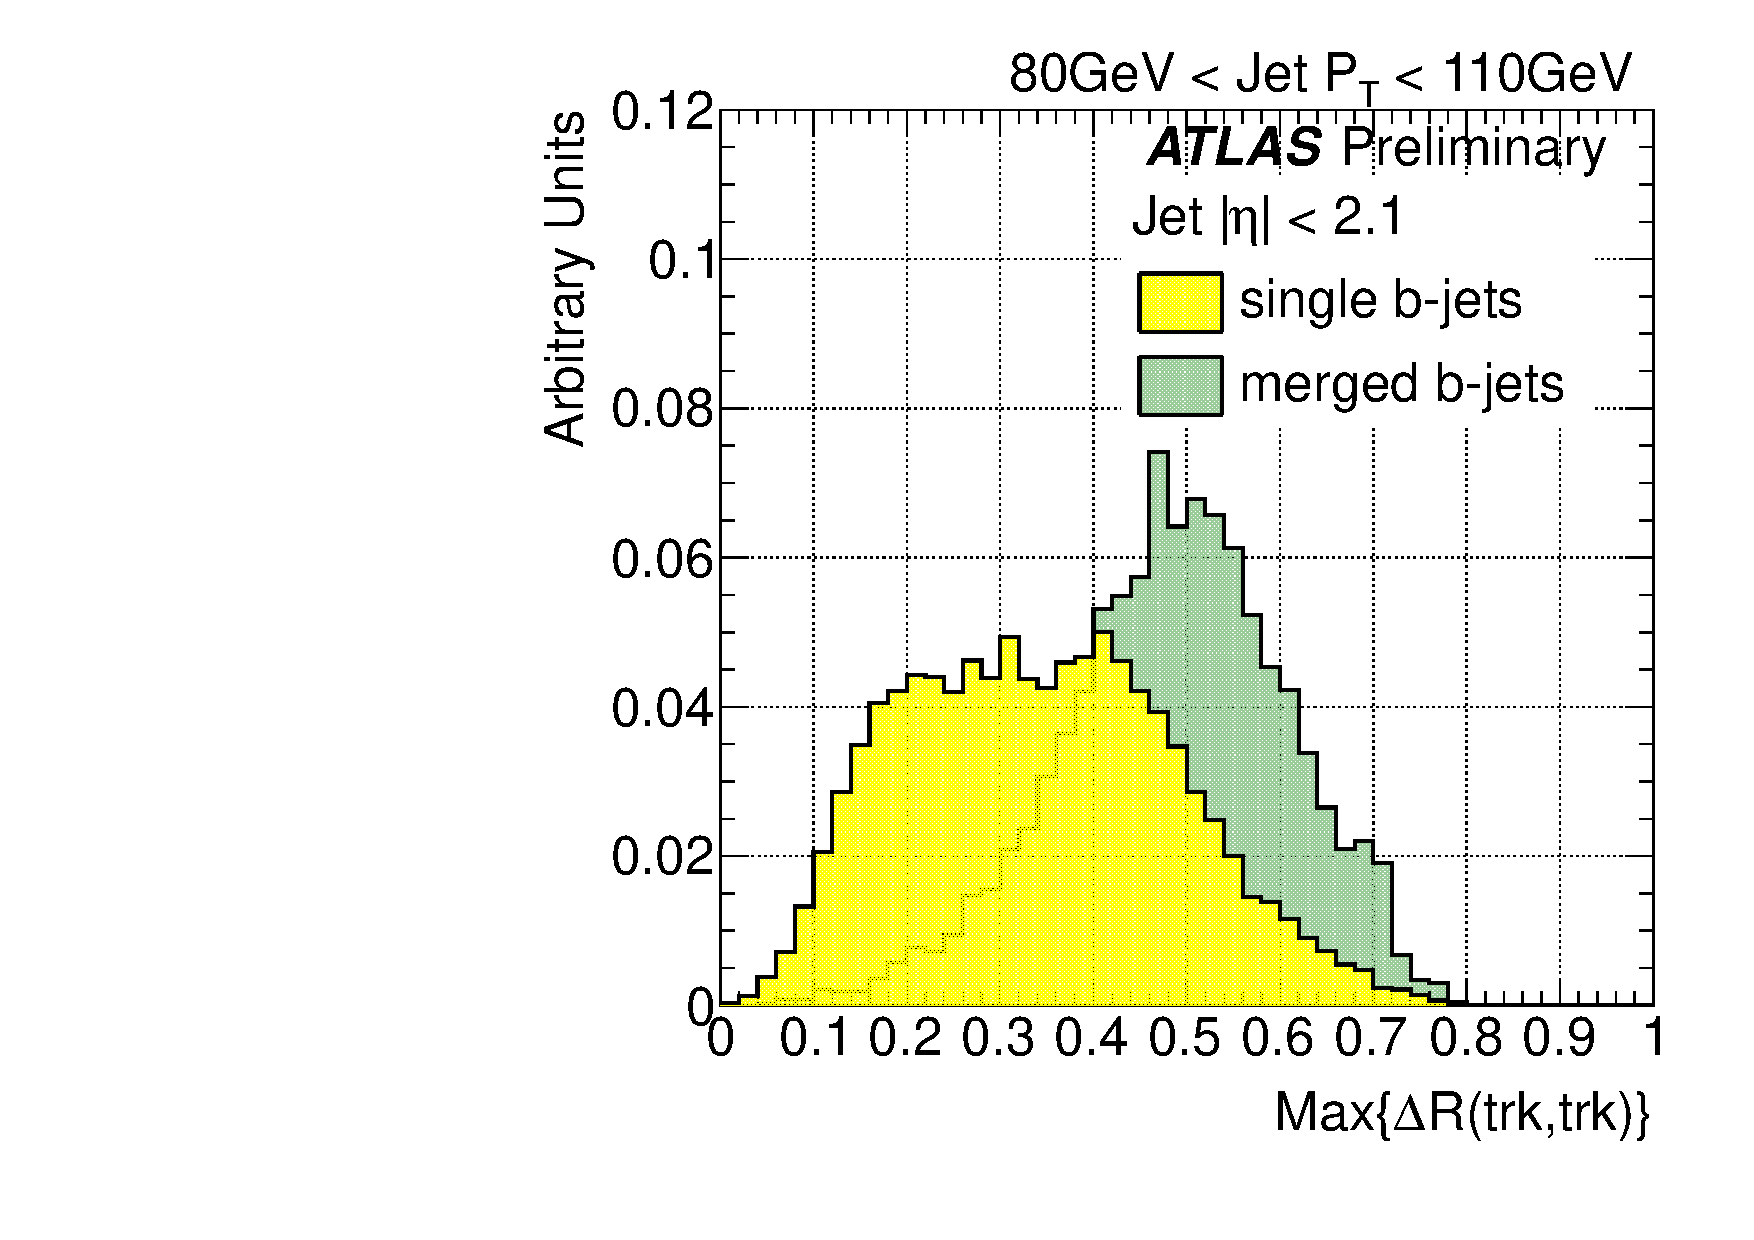
\includegraphics[width=0.49\textwidth]{FIGS/VarsSingleMerged/drmax080.pdf}
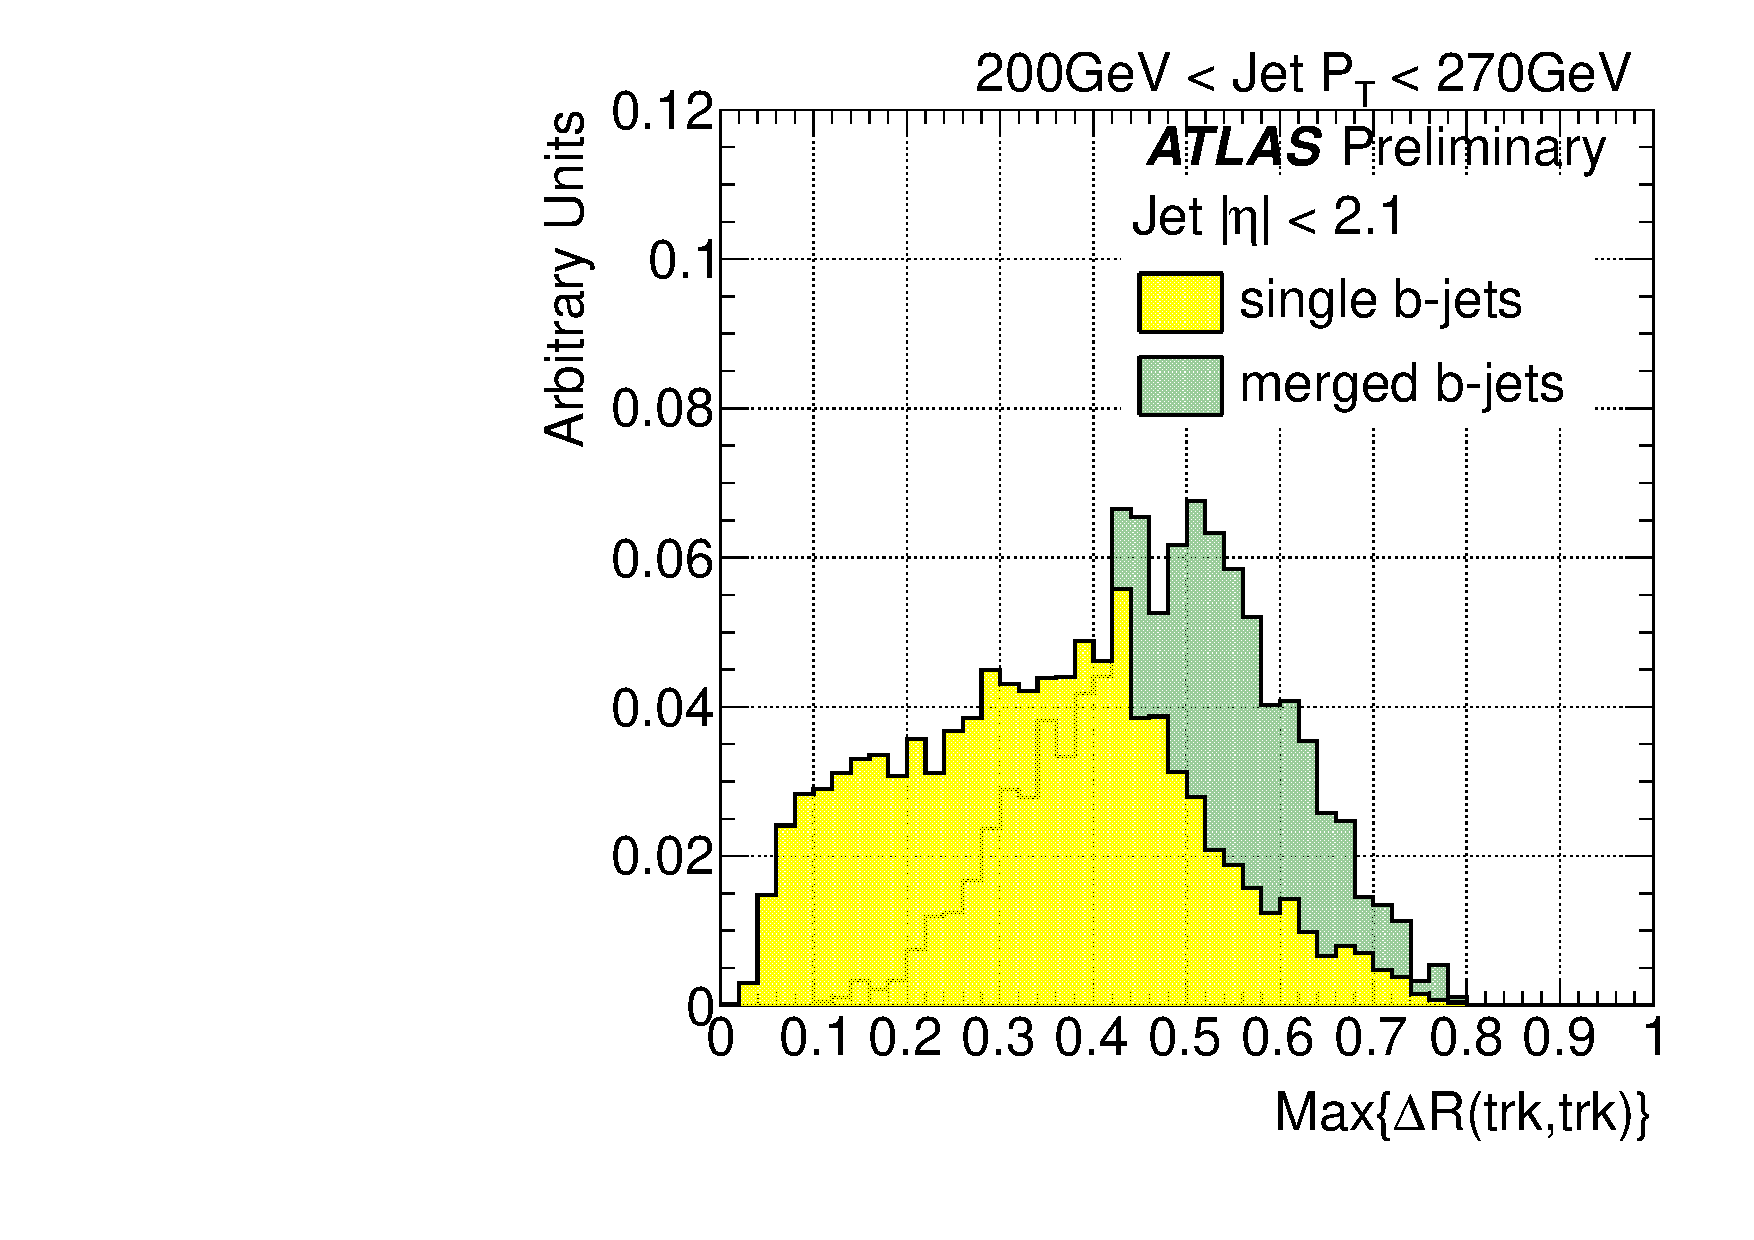
\includegraphics[width=0.49\textwidth]{FIGS/VarsSingleMerged/drmax200.pdf}
\caption{Distribution of the maximum $\Delta R$ between pairs of tracks in jets for single and merged $b$-jets between 80~GeV to 110~GeV (left) and 200~GeV to 270~GeV (right).}
\label{fig:drmaxsinglemerged}
\end{figure}


{ \em IV. $\Delta R$ between the axes of two $k_t$ subjets}
\\[3mm]
The distribution of the $\Delta R$ between the axes of the two exclusive $k_t$ subjets in the jet is shown in Fig.~\ref{fig:drktsinglemerged} for single and merged $b$-jets. In order to build this variable the $k_t$ algorithm~\cite{kt1} is applied to all the tracks associated to the jet using a large $k_t$  distance parameter to ensure that all of them get clustered. The clustering is stopped once it reaches exactly two jets. We observe that this variable also provides good separation, with the advantage of infrared safeness and insensitivity to pile-up. % revealing the two-prong substructure of merged $b$-jets.
\\[3mm]

\begin{figure}[tp]
\centering
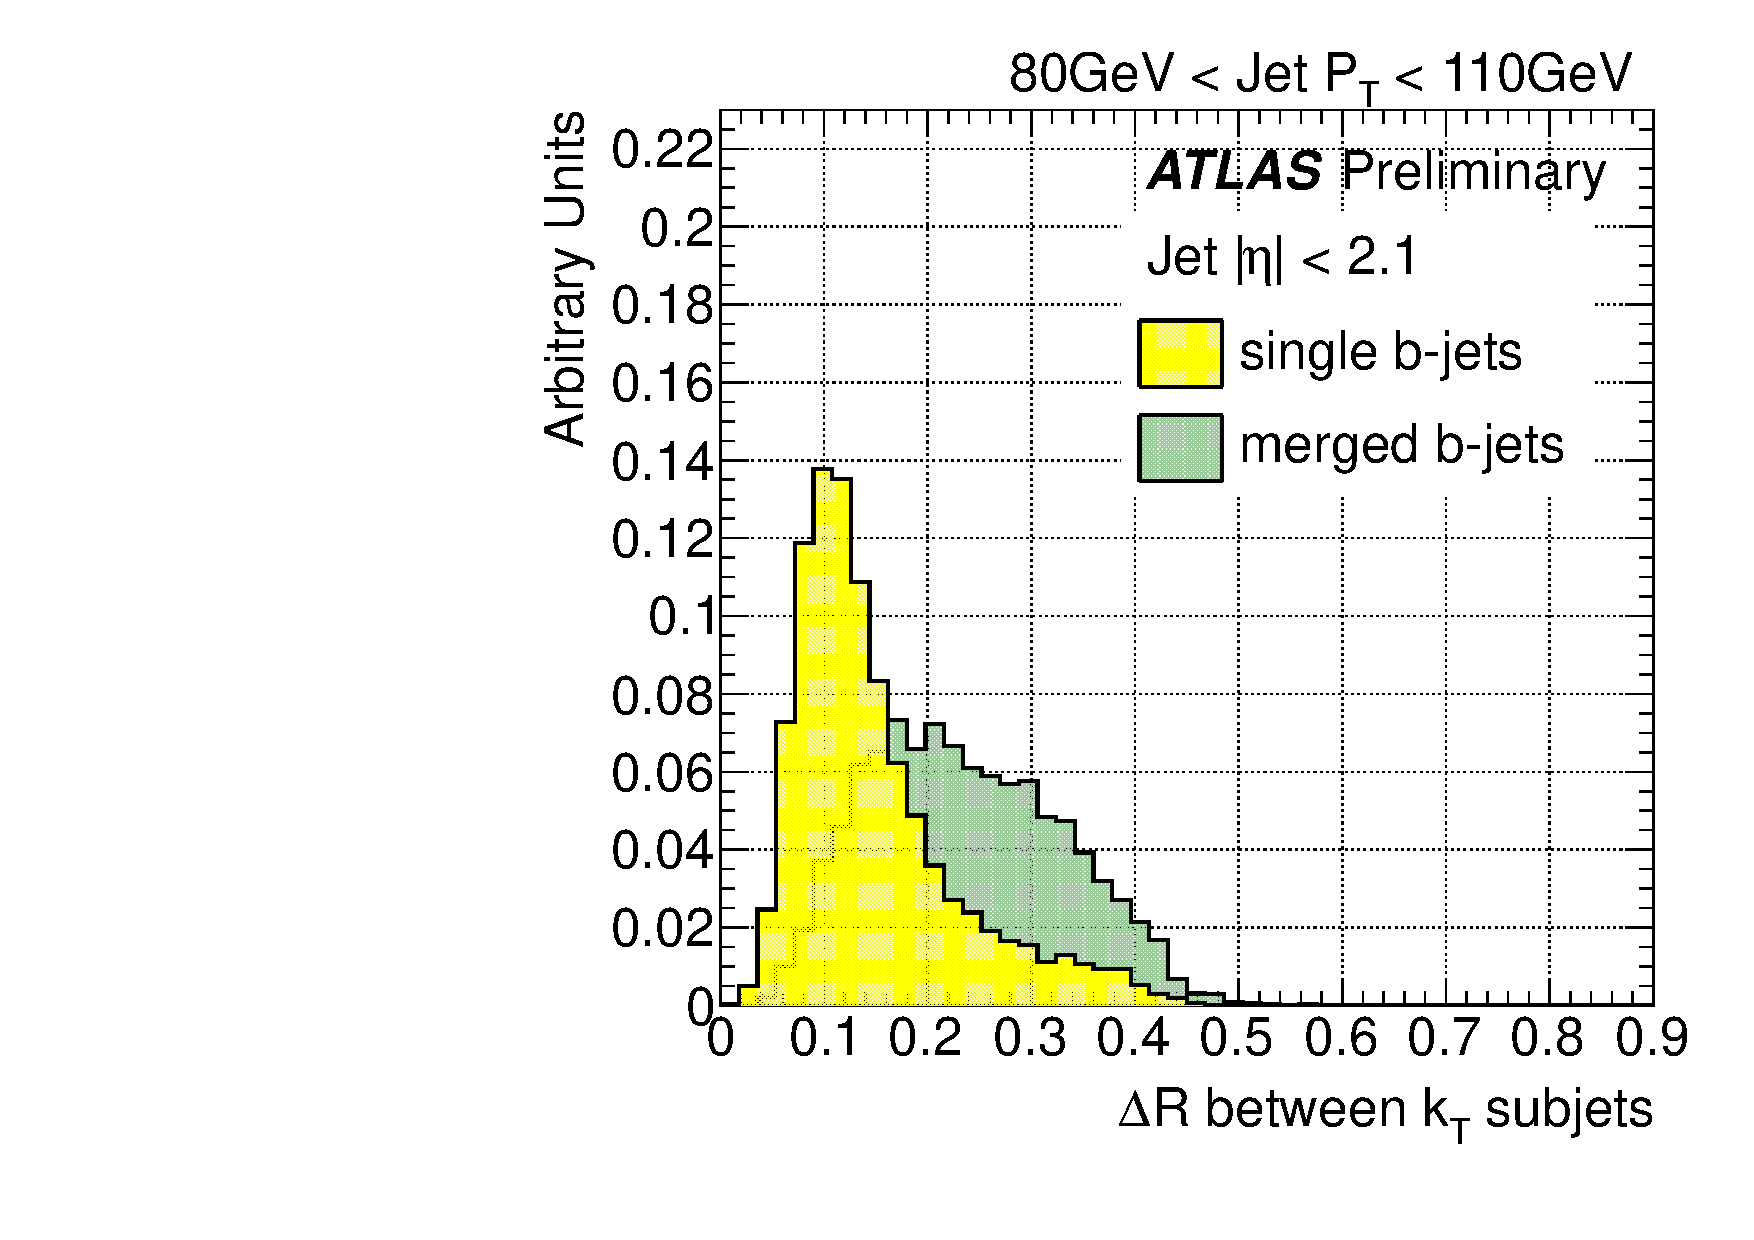
\includegraphics[width=0.49\textwidth]{FIGS/VarsSingleMerged/DRkt2axes080.pdf}
\includegraphics[width=0.49\textwidth]{FIGS/VarsSingleMerged/DRkt2axes200.pdf}
\caption{Distribution of the $\Delta R$ between the axes of the two $k_t$ subjets in the jet for single and merged $b$-jets between 80~GeV to 110~GeV (left) and 200~GeV to 270~GeV (right).}
\label{fig:drktsinglemerged}
\end{figure}


{ \em V. $N$-subjettiness variables}
\\[3mm]

$N$-subjettiness variables, as described in Ref.~\cite{nsubjettiness}, were originally designed to identify boosted objects, like electroweak bosons and top quarks, decaying into collimated shower of hadrons which a standard jet algorithm would reconstruct as single jets. It is defined as:
\begin{equation} 
\tau_N = \frac{1}{\sum_k {\pt}_k\,R_0} \sum_k {\pt}_k \min \{ \Delta R_{S_1,k},\,\Delta R_{S_2,k},...,\,\Delta R_{S_N,k} \}
\end{equation} 
where $R_0$ is the jet radius used in the jet clustering algorithm and the sum runs over the constituents of the jet. To avoid dependence on pile-up we consider the track-based $n$-subjettiness, where the sum 
 is over the tracks in the $b$-tagged jet. $\Delta R_{S_j,k} $ is the distance in the rapidity-azimuth plane between the axis of subjet $j$ and constituent track $k$. This jet shape variable quantifies to what degree a jet can be regarded as composed of $N$ subjets. For instance, a jet with a two pronged structure, with all tracks clustered along two directions, is expected to have a smaller $\tau_2$ value than a jet with tracks uniformly distributed in $\eta-\phi$ space.

Plots of $ \tau_2$ are shown in Fig.~\ref{fig:tau2singlemerged}. In spite of its expected 2-prong substructure, merged $b$-jets have higher values of $ \tau_2$ than single $b$-jets. The explanation of this behavior can be found in Fig.~\ref{fig:tau2trkwidthsinglemerged}, where its correlation with  track-jet width ($\sim \tau_1$) is shown for single and merged $b$-jets. The two variables are highly correlated and for this reason wider jets  have a larger $ \tau_2$. This suggests to switch from an absolute to a width-normalized
$\tau_2$. Fig.~\ref{fig:tauratiosinglemerged} thus shows the distributions of $\tau_2/\tau_1$. This ratio is often used but, although as expected somewhat larger values are obtained for single than for merged $b$-jets, specially at high $\pt$, we decided not to use this variable as it offers only marginal discrimination. 
\\[3mm]

\begin{figure}[tp]
\centering
\includegraphics[width=0.49\textwidth]{FIGS/VarsSingleMerged/Tau2080.pdf}
\includegraphics[width=0.49\textwidth]{FIGS/VarsSingleMerged/Tau2200.pdf}
\caption{Distribution of $\tau_2$ in jets for single and merged $b$-jets between 80~GeV to 110~GeV (left) and 200~GeV to 270~GeV (right).}
\label{fig:tau2singlemerged}
\end{figure}


\begin{figure}[tp]
\centering
\includegraphics[width=0.49\textwidth]{FIGS/VarsSingleMerged/Tau2trkWidth080.pdf}
\includegraphics[width=0.49\textwidth]{FIGS/VarsSingleMerged/Tau2trkWidth200.pdf}
\caption{Correlation between $\tau _2$ and track-jet width for single and merged $b$-jets between 80~GeV to 110~GeV (left) and 200~GeV to 270~GeV (right).}
\label{fig:tau2trkwidthsinglemerged}
\end{figure}

\begin{figure}[tp]
\centering
\includegraphics[width=0.49\textwidth]{FIGS/VarsSingleMerged/TauRatio080.pdf}
\includegraphics[width=0.49\textwidth]{FIGS/VarsSingleMerged/TauRatio200.pdf}
\caption{Distribution of $\tau_2/\tau_1$ in jets for single and merged $b$-jets between 80~GeV to 110~GeV (left) and 200~GeV to 270~GeV (right).}
\label{fig:tauratiosinglemerged}
\end{figure}


%Variables such as the $\DeltaR$ between the two leading constituents of the jet (those with highest transverse momentum) and the jet eccentricity (the ratio of the principal axes of the jet area) did not show good discrimination either and were not considered for the multivariate study.

{ \em VI. Jet Mass}
\\[3mm]

Figure~\ref{fig:masssinglemerged} shows the distribution of the jet mass for single and merged $b$-jets.
\\[3mm]

\begin{figure}[tp]
\centering
\includegraphics[width=0.49\textwidth]{FIGS/VarsSingleMerged/JetMass080.pdf}
\includegraphics[width=0.49\textwidth]{FIGS/VarsSingleMerged/JetMass200.pdf}
\caption{Distribution of jet mass in~GeV for single and merged $b$-jets between 80~GeV to 110~GeV (left) and 200~GeV to 270~GeV (right).}
\label{fig:masssinglemerged}
\end{figure}

{ \em VII. Number of $k_t$ subjets}
\\[3mm]

Figure~\ref{fig:nsubjetsinglemerged} shows the distribution of the number of sub-track-jets single and merged $b$-jets.
\\[3mm]

\begin{figure}[tp]
\centering
\includegraphics[width=0.49\textwidth]{FIGS/VarsSingleMerged/Nsubjets080.pdf}
\includegraphics[width=0.49\textwidth]{FIGS/VarsSingleMerged/Nsubjets200.pdf}
\caption{Distribution of the number of $k_t$ sub-track-jets for single and merged $b$-jets between 80~GeV to 110~GeV (left) and 200~GeV to 270~GeV (right).}
\label{fig:nsubjetsinglemerged}
\end{figure}


{ \em VIII. $\Delta R$ between leading constituents}
\\[3mm]

Figure~\ref{fig:drtrk12singlemerged} shows the distribution of the number  $\Delta R$ between leading tracks in the jet for single and merged $b$-jets.
\\[3mm]

\begin{figure}[tp]
\centering
\includegraphics[width=0.49\textwidth]{FIGS/VarsSingleMerged/DRtrk12080.pdf}
\includegraphics[width=0.49\textwidth]{FIGS/VarsSingleMerged/DRtrk12200.pdf}
\caption{Distribution of $\Delta R$ between leading tracks for single and merged $b$-jets between 80~GeV to 110~GeV (left) and 200~GeV to 270~GeV (right).}
\label{fig:drtrk12singlemerged}
\end{figure}


{ \em IX. Jet eccentricity}
\\[3mm]

Figure~\ref{fig:jeteccsinglemerged} shows the distribution of the jet track-eccentricity for single and merged $b$-jets.
\\[3mm]

\begin{figure}[tp]
\centering
\includegraphics[width=0.49\textwidth]{FIGS/VarsSingleMerged/JetEcc080.pdf}
\includegraphics[width=0.49\textwidth]{FIGS/VarsSingleMerged/JetEcc200.pdf}
\caption{Distribution of the jet eccentricity for single and merged $b$-jets between 80~GeV to 110~GeV (left) and 200~GeV to 270~GeV (right).}
\label{fig:jeteccsinglemerged}
\end{figure}


We also explored the potential improvement of constructing kinematic variables with only displaced tracks, as these are the ones expected to arise from the decay of B-hadrons. Cuts of 2, 2.5 and 3 on the track transverse impact parameter significance were investigated leading however to no gain in discrimation power.

 In Figures~\ref{fig:displacedntrk} and~\ref{fig:displacedtrkwidth} two examples are shown.

\begin{figure}[tp]
\centering
\includegraphics[width=0.49\textwidth]{FIGS/TEMPFigs/DisplacedTracks/ntrk_singlemerged_AllandDisplaced_80-120.pdf}
\includegraphics[width=0.49\textwidth]{FIGS/TEMPFigs/DisplacedTracks/ntrk_singlemerged_AllandDisplaced_260-310.pdf}
\caption{Distribution of the jet track multiplicity single and merged $b$-jets between 80~GeV to 110~GeV (left) and 200~GeV to 270~GeV (right), for all and displaced tracks only.}
\label{fig:displacedntrk}
\end{figure}


\begin{figure}[tp]
\centering
\includegraphics[width=0.49\textwidth]{FIGS/TEMPFigs/DisplacedTracks/trkWidth_singlemerged_AllandDisplaced_80-120.pdf}
\includegraphics[width=0.49\textwidth]{FIGS/TEMPFigs/DisplacedTracks/trkWidth_singlemerged_AllandDisplaced_260-310.pdf}
\caption{Distribution of the track-jet width for single and merged $b$-jets between 80~GeV to 110~GeV (left) and 200~GeV to 270~GeV (right), for all and displaced tracks only.}
\label{fig:displacedtrkwidth}
\end{figure}


\subsection{Further studies using ``ghost-association'' and bigger cone jets}

In order to better understand the behavior observed for $\tau_2$, $\Delta R$ between the axes of $k_T$ subjets and jet eccentricity in anti-$k_T$ 0.4 jets, these variables were studied for other two different scenarios,

\begin{itemize}\addtolength{\itemsep}{-0.4\baselineskip}
\item 
using the active area of jets (with clusters used as input to jet reconstruction).
\item
using bigger 0.6 anti-$k_T$ jets
\end{itemize}
%
in order to enhance the efficiency to capture the decay products in gluon to $b \bar{b}$-jets.

Figures~\ref{fig:tau2GhostAndAntikt6} to~\ref{fig:jeteccGhostAndAntikt6} show distributions of variables mentioned above for single and merged $b$-jets  between 80~GeV to 110~GeV.

\begin{figure}[tp]
\centering
\includegraphics[width=0.49\textwidth]{FIGS/TEMPFigs/Antikt6VarsSingleMerged/Tau2080.pdf}
\includegraphics[width=0.49\textwidth]{FIGS/TEMPFigs/GhostMatchingVarsClus/Tau2080.pdf}
\caption{Distribution of $\tau_2$ for single and merged $b$-jets between 80~GeV to 110~GeV in anti-$k_T$ 0.6 jets using track constituents (left) and anti-$k_T$ 0.4 jets using the active area of the jet, with calorimeter topoclusters as input.}
\label{fig:tau2GhostAndAntikt6}
\end{figure}

\begin{figure}[tp]
\centering
\includegraphics[width=0.49\textwidth]{FIGS/TEMPFigs/Antikt6VarsSingleMerged/DRkt2axes080.pdf}
\includegraphics[width=0.49\textwidth]{FIGS/TEMPFigs/GhostMatchingVarsClus/DRkt2axes080.pdf}
\caption{Distribution of $\Delta R$ between $k_T$ subjets for single and merged $b$-jets between 80~GeV to 110~GeV in anti-$k_T$ 0.6 jets using track constituents (left) and anti-$k_T$ 0.4 jets using the active area of the jet, with calorimeter topoclusters as input.}
\label{fig:drktaxisGhostAndAntikt6}
\end{figure}

\begin{figure}[tp]
\centering
\includegraphics[width=0.49\textwidth]{FIGS/TEMPFigs/Antikt6VarsSingleMerged/JetTrackEccentricity080.pdf}
\includegraphics[width=0.49\textwidth]{FIGS/TEMPFigs/GhostMatchingVarsClus/JetCaloEccentricity080.pdf}
\caption{Distribution of the jet eccentricity for single and merged $b$-jets between 80~GeV to 110~GeV in anti-$k_T$ 0.6 jets using track constituents (left) and anti-$k_T$ 0.4 jets using the active area of the jet, with calorimeter topoclusters as input.}
\label{fig:jeteccGhostAndAntikt6}
\end{figure}




%------------------------------------------------------------------------
\section{Validation of the jet variables in data}\label{sec:gbbValidation}
%------------------------------------------------------------------------

 In order to study the extent to which the simulation reproduces the distributions observed in data for the different variables explored a set of comparison plots is presented. Fig.~\ref{fig:datamcinputvars} shows the distributions of jet track multiplicity, track-jet width and $\Delta R$ between the axes of the two $k_t$ subjets, in two different jet $\pt$ bins in dijet Monte Carlo and data events collected by ATLAS %until summer 2011 ($\mu \approx 6$) overlaid.
during 2011. The distributions are normalized to unit area to allow for shape comparisons. There is a good agreement between data and simulation. It should be remarked that the observed agreement is actually not a direct validation of the description in the MC of the relevant variables, but its convolution with the simulated relative fractions of light-, $c$-, $b$- and $bb$-jets in the $b$-tagged generated jet sample. To some extent, some level of compensation can take place between these two effects.

% For the sake of evaluating the effect of the increasing amount of pile-up in the last period of data-taking, %affected the agreement between experimental data and Monte Carlo
%the same distributions were built using data events recorded in the second half of the year ($\mu \approx 12$).  As expected, no significant variation was observed. In Fig.~\ref{fig:datamcinputvarsItoM} the jet track multiplicity is shown for this period, in the same two $\pt$ bins for comparison.  

\begin{figure}[tp]
\centering
\includegraphics[width=0.49\textwidth]{FIGS/dataMC/FullDataVarNtrkPT080.pdf}
\includegraphics[width=0.49\textwidth]{FIGS/dataMC/FullDataVarNtrkPT200.pdf}
\includegraphics[width=0.49\textwidth]{FIGS/dataMC/FullDataVarTrkWidthPT080.pdf}
\includegraphics[width=0.49\textwidth]{FIGS/dataMC/FullDataVarTrkWidthPT200.pdf}  
\includegraphics[width=0.49\textwidth]{FIGS/dataMC/FullDataVarDRktaxisPT080.pdf}
\includegraphics[width=0.49\textwidth]{FIGS/dataMC/FullDataVarDRktaxisPT200.pdf}  
%\caption{ Distribution of three tracking variables in 2 different jet $\pt$ bins, for experimental data  collected by ATLAS until summer 2011, with $\mu \approx 6$ (solid black points), and simulated data (filled histograms). The ratio data over simulation is shown at the bottom of each plot.}
\caption{ Distribution of three tracking variables in 2 different jet $\pt$ bins, for experimental data  collected by ATLAS during 2011 (solid black points), and simulated data (filled histograms). The ratio data over simulation is shown at the bottom of each plot.}
\label{fig:datamcinputvars}
\end{figure}


%\begin{figure}[tp]
%\centering
%\includegraphics[width=0.49\textwidth]{FIGS/dataMCItoM/VarNtrkPT080.pdf}
%\includegraphics[width=0.49\textwidth]{FIGS/dataMCItoM/VarNtrkPT200.pdf}
%\caption{ Distribution of the jet track-multiplicity in 2 different jet $\pt$ bins, for experimental data from the last period of data-taking, with $\mu \approx 12$ (solid black points), and simulated data (filled histograms). The ratio data over simulation is shown at the bottom of each plot.}
%\label{fig:datamcinputvarsItoM}
%\end{figure}




%
%%%%%%%%%%%%%%%%%%%%%%%%%%%%%%%%%%%%%%%%%%%%%%%%%%%%%%%%%%%%%%%%%%%%%%%%%%%%%%%
% Multivariate Analysis
%%%%%%%%%%%%%%%%%%%%%%%%%%%%%%%%%%%%%%%%%%%%%%%%%%%%%%%%%%%%%%%%%%%%%%%%%%%%%%%
%
\chapter{Multivariate Analysis}\label{sec:gbbTMVA}


%------------------------------------------------------------------------
\section{The multivariate classifiers}
%------------------------------------------------------------------------

The following multivariate methods were explored:

\begin{itemize}\addtolength{\itemsep}{-0.4\baselineskip}
\item
Likelihood ratio estimators 
\item
Neural Networks (NN)
\item
Boosted decision Trees (BDTs)
\end{itemize}

And different trainings were tested:

\begin{itemize}\addtolength{\itemsep}{-0.4\baselineskip}
\item
Inclusive, with $\pt$-weighting
\item
In bins of jet $\pt$
\end{itemize}


Signal and background jets were not weighted by the dijet samples cross-sections to allow the contribution of subleading lower $\pt$ jets from high $\pt$ events, and thus increase the statistics of merged jets in the low $\pt$ bins. 


Figure~\ref{fig:diffmethodsInclusive} and~\ref{fig:diffmethodsBins} show distributions of the MVA outputs in different bins of jet $\pt$ for the two proposed trainings. In figures~\ref{fig:diffmethodsPerfInclusive} and~\ref{fig:diffmethodsPerfBins} a comparison of the performance of all methods, for inclusive and ``in-bins'', training is illustrated.


\begin{figure}[tp]
\centering
\includegraphics[width=0.32\textwidth]{FIGS/TEMPFigs/MVA_differentMethods/inclusive/NNoutput040_LihoodKDE.pdf}
\includegraphics[width=0.32\textwidth]{FIGS/TEMPFigs/MVA_differentMethods/inclusive/NNoutput080_LihoodKDE.pdf}
\includegraphics[width=0.32\textwidth]{FIGS/TEMPFigs/MVA_differentMethods/inclusive/NNoutput200_LihoodKDE.pdf}
\includegraphics[width=0.32\textwidth]{FIGS/TEMPFigs/MVA_differentMethods/inclusive/NNoutput040_MLP.pdf}
\includegraphics[width=0.32\textwidth]{FIGS/TEMPFigs/MVA_differentMethods/inclusive/NNoutput080_MLP.pdf}
\includegraphics[width=0.32\textwidth]{FIGS/TEMPFigs/MVA_differentMethods/inclusive/NNoutput200_MLP.pdf}
\includegraphics[width=0.32\textwidth]{FIGS/TEMPFigs/MVA_differentMethods/inclusive/NNoutput040_BDT.pdf}
\includegraphics[width=0.32\textwidth]{FIGS/TEMPFigs/MVA_differentMethods/inclusive/NNoutput080_BDT.pdf}
\includegraphics[width=0.32\textwidth]{FIGS/TEMPFigs/MVA_differentMethods/inclusive/NNoutput200_BDT.pdf}
\caption{Distribution of the MVA discriminant outputs, for inclusive training, in single and merged $b$-jets, for low, medium and high jet $\pt$.}
\label{fig:diffmethodsInclusive}
\end{figure}

\begin{figure}[tp]
\centering
\includegraphics[width=0.32\textwidth]{FIGS/TEMPFigs/MVA_differentMethods/bins/NNoutput040_LihoodKDE.pdf}
\includegraphics[width=0.32\textwidth]{FIGS/TEMPFigs/MVA_differentMethods/bins/NNoutput080_LihoodKDE.pdf}
\includegraphics[width=0.32\textwidth]{FIGS/TEMPFigs/MVA_differentMethods/bins/NNoutput200_LihoodKDE.pdf}
\includegraphics[width=0.32\textwidth]{FIGS/TEMPFigs/MVA_differentMethods/bins/NNoutput040_MLP.pdf}
\includegraphics[width=0.32\textwidth]{FIGS/TEMPFigs/MVA_differentMethods/bins/NNoutput080_MLP.pdf}
\includegraphics[width=0.32\textwidth]{FIGS/TEMPFigs/MVA_differentMethods/bins/NNoutput200_MLP.pdf}
\includegraphics[width=0.32\textwidth]{FIGS/TEMPFigs/MVA_differentMethods/bins/NNoutput040_BDT.pdf}
\includegraphics[width=0.32\textwidth]{FIGS/TEMPFigs/MVA_differentMethods/bins/NNoutput080_BDT.pdf}
\includegraphics[width=0.32\textwidth]{FIGS/TEMPFigs/MVA_differentMethods/bins/NNoutput200_BDT.pdf}
\caption{Distribution of the MVA discriminant outputs, for training in bins of jet $\pt$, in single and merged $b$-jets, for low, medium and high jet $\pt$.}
\label{fig:diffmethodsBins}
\end{figure}

\begin{figure}[tp]
\centering
\includegraphics[width=0.49\textwidth]{FIGS/TEMPFigs/MVA_differentMethods/inclusive/MVAs_RejvsEff40.pdf}
\includegraphics[width=0.49\textwidth]{FIGS/TEMPFigs/MVA_differentMethods/inclusive/MVAs_RejvsEff200.pdf}
\caption{Distribution of the MVA discriminant performance for inclusive training, in single and merged $b$-jets, for low and high jet $\pt$.}
\label{fig:diffmethodsPerfInclusive}
\end{figure}

\begin{figure}[tp]
\centering
\includegraphics[width=0.49\textwidth]{FIGS/TEMPFigs/MVA_differentMethods/bins/MVAs_RejvsEff40.pdf}
\includegraphics[width=0.49\textwidth]{FIGS/TEMPFigs/MVA_differentMethods/bins/MVAs_RejvsEff200.pdf}
\caption{Distribution of the MVA discriminant performance for training in bins of jet $\pt$, in single and merged $b$-jets, for low and high jet $\pt$.}
\label{fig:diffmethodsPerfBins}
\end{figure}

%------------------------------------------------------------------------
\section{The input variables}
%------------------------------------------------------------------------

Different groups of input variables were tested. Figure~\ref{fig:difftrainings} shows the performance for three sets of variables for MVA classifier.

\begin{figure}[tp]
\centering
\includegraphics[width=0.32\textwidth]{FIGS/TEMPFigs/MVA_differentTrainings/DiffTrainings_RejvsEff40.pdf}
\includegraphics[width=0.32\textwidth]{FIGS/TEMPFigs/MVA_differentTrainings/DiffTrainings_RejvsEff80.pdf}
\includegraphics[width=0.32\textwidth]{FIGS/TEMPFigs/MVA_differentTrainings/DiffTrainings_RejvsEff200.pdf}
\caption{Distribution of the MVA discriminant performance for three sets of input variables, in single and merged $b$-jets, for low, medium and high jet $\pt$.}
\label{fig:outputinbin}
\end{figure}

%------------------------------------------------------------------------
\section{$\bm{ g\rightarrow b\bar{b}}$ likelihood training and performance}
%------------------------------------------------------------------------

A discriminant between single $b$-jets and merged $b$-jets was built by training a simple likelihood estimator in the context of the Toolkit for Multivariate Data Analysis, TMVA~\cite{Hocker:2007ht}.

A sub-set of the dijet Monte Carlo sample was used for training. After the event and jet selections were performed, the $b$-tagged jets with $|\eta| < 2.1$ were classified as signal (single $b$-jets) or background (merged $b$). % depending on whether one or two $B$-hadrons were found within a 0.4 cone around the jet axis. %For the evaluation of the method the same procedure was followed.
The likelihood training was done in bins of calorimeter jet $\pt$. % and only isolated jets were considered. 
Signal and background jets were not weighted by the dijet samples cross-sections to allow the contribution of subleading lower $\pt$ jets from high $\pt$ events, and thus increase the statistics of merged jets in the low $\pt$ bins. For the evaluation of the method the same procedure was followed.

Several combinations of the tracking and jet shape variables studied in the previous section were tested as input variables. We found that the following three offer the best performance:
% that the jet track multiplicity, the track-jet width and $\Delta R$  between the axes of the two $k_t$ subjets offered the best performance. 
\begin{enumerate}\addtolength{\itemsep}{-0.4\baselineskip}
\item
Jet track multiplicity
\item
Track-jet width
\item
$\Delta R$ between the axes of 2 $k_t$ subjets within the jet
\end{enumerate}
%
A requirement of at least two matching tracks was imposed to all $b$-tagged jets in order to build the third variable listed. This cut was applied in both training and testing samples.

The distribution of the likelihood output for single and merged $b$-jets is shown in  Fig.~\ref{fig:outputinbins} for low, medium and high transverse momentum jets.

\begin{figure}[tp]
\centering
\includegraphics[width=0.32\textwidth,viewport=40 0 540 550]{FIGS/Likelihood/NNoutput040_LihoodKDE.pdf}
%\includegraphics[width=0.32\textwidth]{FIGS/Likelihood/NNoutput040_LihoodKDE.pdf}
\includegraphics[width=0.32\textwidth,viewport=40 0 540 550,clip]{FIGS/Likelihood/NNoutput080_LihoodKDE.pdf}
\includegraphics[width=0.32\textwidth,viewport=40 0 540 550,clip]{FIGS/Likelihood/NNoutput200_LihoodKDE.pdf}  
\caption{Distribution of the $g\rightarrow b \bar{b}$ likelihood output for single and merged $b$-jets for low, medium and high $\pt$ jets.}
\label{fig:outputinbins}
\end{figure}

The performance of the $g\rightarrow b \bar{b}$ tagger in the simulation can be  %seen in Fig.~\ref{fig:performanceinbins}. In this plot the rejection ($1/\epsilon_{bkg}$) of merged $b$-jets from gluon splitting is shown as a function of single $b$-jet efficiency for the eight bins of jet $\pt$ mentioned in section~\ref{sec:EventSelection}. The performance improves with $\pt$:
displayed in a plot of rejection ($1/\epsilon_{bkg}$) of merged $b$-jets as a function of single $b$-jet efficiency, where $\epsilon_{bkg}$ is the probability that a $b \bar{b}$-jet passes the tagger. This is shown in Fig.~\ref{fig:performanceinbins} for the eight bins of jet $\pt$ mentioned in section~\ref{sec:EventSelection}. The performance improves with $\pt$:


\begin{itemize}\addtolength{\itemsep}{-0.4\baselineskip}
\item
$\pt>40$ GeV: %\\[1mm]
rejection above 8 at 50\% eff.
% over 85\% rejection at 50\% eff.
\item
$\pt>60$ GeV: %\\[1mm]
rejection above 10 at 50\% eff.
 %90\% rejection at 50\% eff.
\item
$\pt>200$ GeV: %\\[1mm]
rejection above 30 at 50\% eff.
 %over 95\% rejection at 50\% eff.
\end{itemize}


\begin{figure}[tp]
\centering
\includegraphics[width=0.7\textwidth]{FIGS/Likelihood/KDE_RejvsEff.pdf}
\caption{Rejection of $g\rightarrow b \bar{b}$ merged $b$-jets as a function of $b$-jet efficiency for dijet events in 8 jet $\pt$ bins.}
\label{fig:performanceinbins}
\end{figure}

The likelihood was trained with jets that had been first tagged by the MV1 algorithm. In order to use the  $g\rightarrow b \bar{b}$ classifier for jets tagged by another tagger a new training is required.

The rejection of merged jets attained as a function of $\pt$ for the 50\% and 60\% efficiency working points are summarized in Table~\ref{tb:rejection}, together with their relative statistical error. These are propagated from the Poisson fluctuations of the number of events in the merged and single $b\bar{b}$ distributions. The error is slightly lower for the 60\% efficiency working point because a higher efficiency allows for a greater number of Monte Carlo events to measure the performance. %the higher the efficiency, the larger the number of Monte Carlo events available to measure the performance.



\begin{table}[!hbt] %[h]
\renewcommand{\arraystretch}{1.2}
\centering
\begin{tabular}{ | c || c | c || c | c||}
  \hline
  Jet $\pt$ & \multicolumn{2}{c||}{single $b$-jet efficiency 50\%} & 
            \multicolumn{2}{c||}{single $b$-jet efficiency 60\%}\\ \cline{2-5}
    (GeV )  & Rejection & ~stat.err.~ & Rejection & ~stat.err.~ \\ \hline
%   40 - 60 &  ~7.6 &  4\%  &  ~5.4  &  3\%    \\ 
%   60 - 80 &  10.4 &  4\%  &  ~7.3  &  4\%    \\ 
%   80 - 110&  13.9 &  5\%  &  ~9.4  &  4\%    \\ 
%  110 - 150&  18.7 &  5\%  &  12.0  &  4\%    \\ 
%  150 - 200&  23.2 &  5\%  &  14.0  &  5\%    \\ 
%  200 - 270&  29.5 &  7\%  &  15.6  &  6\%    \\ 
%  270 - 360&  36.4 &  7\%  &  18.7  &  6\%    \\ 
%  360 - 480&  41.4 &  8\%  &  18.2  &  8\%    \\ \hline
   40 - 60 &  ~8 &  4\%  &  ~5  &  3\%    \\ 
   60 - 80 &  ~10 &  4\%  &  ~7  &  4\%    \\ 
   80 - 110&  ~14 &  5\%  &  ~9  &  4\%    \\ 
  110 - 150&  19 &  5\%  &  12  &  4\%    \\ 
  150 - 200&  23 &  5\%  &  14  &  5\%    \\ 
  200 - 270&  30 &  7\%  &  16  &  6\%    \\ 
  270 - 360&  36 &  7\%  &  19  &  6\%    \\ 
  360 - 480&  41 &  8\%  &  18  &  8\%    \\ \hline
\end{tabular}
\caption{The merged $b$-jet rejection for the 50\% and 60\% efficiency working points in bins of $\pt$.}
\label{tb:rejection}
\end{table}







%------------------------------------------------------------------------
\section{Systematic uncertainties}\label{sec:gbbSystematics}
%------------------------------------------------------------------------

The development, training and performance determination of the tagger is based on simulated events. Although the agreement between simulation and data explored in section~\ref{sec:validation} is a necessary validation condition, it is also important to investigate how the tagger performance depends on systematics relevant in the data. In particular we have considered:
%
%There are uncertainties in the data that, although not spoiling the data/MC agreement, might change the performance of the tagger. This uncertainties would also be present in an eventual future data-driven determination of the performance as  the data are not known better that this.The following systematic effects have been studied and their influence on the tagger performance ascertained:
%
%In order to study the systematic uncertainties in the method the following contributions were evaluated:
\begin{itemize}\addtolength{\itemsep}{-0.4\baselineskip}
\item
presence of additional interactions (pile-up)
\item
uncertainty in the $b$-jet tagging efficiency % and b-jet energy scale?
\item
uncertainty in the track reconstruction efficiency
\item
uncertainty in the track transverse momentum resolution
\item
uncertainty in the jet transverse momentum resolution  
%\item
%the effect of jet isolation
%\item
%other $\Delta R$ cuts for B-labeling and matching
\end{itemize}

{ \em I. Pile-up}
\\[3mm]
  The size of this effect was studied by comparing the performance of the likelihood discriminant with $b$-jets in events with small (1-9) and large (9-20) number of primary vertices. 
The comparison of the performance in these two sub-samples can be seen in Fig.~\ref{fig:performanceinbinsMu}. 
As expected from the use of tracking (as opposed to calorimeter) variables no significant dependence with pile-up is observed within statistics. Of the 16 determinations (2 working points with 8 $\pt$ bins each) of performance differences between high and low number of primary vertices events, it is observed that 6 of them are positive and 10 negative, with a global mean of 0.3\%. We conclude that the effect is negligible compared to other source of uncertainties.
%

\begin{figure}[tp]
\centering
\includegraphics[width=0.49\textwidth]{FIGS/systematics/50BinsLlhoodKDE_ISO_PileUp_rejvseff040.pdf}
\includegraphics[width=0.49\textwidth]{FIGS/systematics/50BinsLlhoodKDE_ISO_PileUp_rejvseff060.pdf}
\caption{Rejection of $g\rightarrow b \bar{b}$ merged b-jets as a function of $b$-jet efficiency in bins of $N_{\rm vtx}$ for two low jet $\pt$ bins.}
\label{fig:performanceinbinsMu}
\end{figure}

\vspace{3mm}
{\em II. b-tagging efficiency} %energy scale and 
\\[3mm]
The performance of heavy-flavor tagging in Monte Carlo events is calibrated to experimental data by means of the scale factors (SFs) measured by the $b$-tagging group. %scale factors defined as the ratio of the heavy-flavor tagging efficiency in data over that in Monte Carlo (MC) for the different jet flavors, and probably also as a function of jet pT and η 
Such a measurement carries a systematic uncertainty, and in order to estimate its effect a conservative approach is followed: %https://twiki.cern.ch/twiki/bin/viewauth/AtlasProtected/BTaggingCalibrationDataInterface
the SFs are varied in all the $\pt$ bins simultaneously by one standard deviation both in the up and down directions. The result of this procedure for the distribution of two of the tracking variables used in our discriminant is illustrated in Fig.~\ref{fig:btaggingSFs}. 

The effect of the $b$-tagging calibration uncertainty on the likelihood peformance is $< 1$\%, negligible with respect to the statistical uncertainty as it can be seen in Fig.~\ref{fig:btaggingSFsPerf}.
This was indeed expected. The scale factors depend on the true flavor of the jet and on its $\pt$, but these are basically constant in the performance determination, which is based on single flavor (true $b$-) jets classified in $\pt$-bins.

%\textwidth,viewport=45 45 696 672,clip
\begin{figure}[tp]
\centering
\includegraphics[width=0.49\textwidth]{FIGS/systematics/BTagCalib_DataVarNtrkPT080.pdf}
%\includegraphics[width=0.49\textwidth]{FIGS/systematics/BTagCalib_DataVarNtrkPT200.pdf}
%\includegraphics[width=0.49\textwidth]{FIGS/systematics/BTagCalib_DataVarTrkWidthPT080.pdf}
%\includegraphics[width=0.49\textwidth]{FIGS/systematics/BTagCalib_DataVarTrkWidthPT200.pdf}
\includegraphics[width=0.49\textwidth]{FIGS/systematics/BTagCalib_DataVarDRktaxisPT080.pdf}
%\includegraphics[width=0.49\textwidth]{FIGS/systematics/BTagCalib_DataVarDRktaxisPT200.pdf}
\caption{The effect of a variation in the $b$-tagging Scale Factors on the tracking variables distributions. Scale Factors were varied up (down) by 1-sigma to evaluate the systematic uncertainty from this source. The ratio data over MC is shown for MC {\sc pythia} with SFs varied up (circles) and down (triangles).}
\label{fig:btaggingSFs}
\end{figure}

\begin{figure}[tp]
\centering
\includegraphics[width=0.49\textwidth]{FIGS/systematics/LlhoodKDE_ISO_BTagCalibTest_rejvseff060.pdf}
\includegraphics[width=0.49\textwidth]{FIGS/systematics/LlhoodKDE_ISO_BTagCalibTest_rejvseff270.pdf}
\caption{Rejection of $g\rightarrow b \bar{b}$ merged b-jets as a function of $b$-jet efficiency with and without scale factors.}
\label{fig:btaggingSFsPerf}
\end{figure}

%

\vspace{3mm}
{ \em III. Track reconstruction efficiency}
\\[3mm]
This uncertainty arises from the limit in the understanding of the material layout of the Inner Detector. To test its impact a fraction of tracks determined from the track efficiency uncertainty was randomly removed following the method in Ref.~\cite{JetMassNote}.%https://cdsweb.cern.ch/record/1344082?ln=en

The tracking efficiency systematics are given in bins of track $\eta$. For tracks with $p_{\rm{T}}^{\rm{track}} > 500$~MeV the uncertainties are independent of $\pt$:  2\% for $|\eta^{\rm{track}}|<1.3$, 3\% for $1.3<|\eta^{\rm{track}}|<1.9$, 4\% for $1.9<|\eta^{\rm{track}}|<2.1$, 4\% for $2.1<|\eta^{\rm{track}}|<2.3$ and 7\% for $2.3<|\eta^{\rm{track}}|<2.5$~\cite{chargemultiplicity}. All numbers are relative to the corresponding tracking efficiencies.  
%https://cdsweb.cern.ch/record/1286839
%http://arxiv.org/abs/1012.5104

The tracking variables were re-calculated and the performance of the nominal likelihood was evaluated in the new sample with worse tracking efficiency. The rejection-efficiency plots, shown in Fig.~\ref{fig:trackefficiency}, show a small degradation of the performance which is comparable to the statistical uncertainty. The effect is however systematically present over all 16 $\pt$ bin/working points, without a clear $\pt$ dependence. We have thus taken the average over $\pt$, and obtained a global systematic uncertainty of 4\% both for the 50\% and 60\% efficiency working points.

\begin{figure}[tp]
\centering
\includegraphics[width=0.49\textwidth]{FIGS/systematics/LlhoodKDE_ISO_TrackingUncertaintyTest_rejvseff080.pdf}
\includegraphics[width=0.49\textwidth]{FIGS/systematics/LlhoodKDE_ISO_TrackingUncertaintyTest_rejvseff200.pdf}
\caption{Rejection of $g\rightarrow b \bar{b}$ merged $b$-jets as a function of $b$-jet efficiency showing shift in likelihood performance caused by a reduction in the tracking efficiency .}
\label{fig:trackefficiency}
\end{figure}

\vspace{3mm}
{\em IV. Track momentum resolution}
\\[3mm]
The knowledge of the track momentum resolution is limited by the precision both in the material description of the Inner Detector and in the mapping of the magnetic field. Its uncertainty propagates to the kinematic variables used in the 
$g\rightarrow b \bar{b}$ tagger. In order to study this effect, track momenta are over-smeared according to the measured resolution uncertainties before computing the rejection. The actual smearing is done in 1/$\pt$, with an upper bound to the resolution uncertainty given by $\sigma$(1/$\pt$)=0.02/$\pt$~\cite{ATLAS-CONF-2010-009}. The effect is found to be negligible. %with respect to the statistical uncertainty.

\vspace{3mm}
{ \em V. Jet transverse momentum resolution}
\\[3mm]
The jet momentum resolution was measured for 2011 data and found to be in agreement with the predictions from the {\sc pythia8}-based simulation~\cite{JER2011}. The precision of this measurement, determined in $\pt$ and $\eta$ bins,is typically 10\%.
The systematic uncertainty due to the calorimeter jet $\pt$ resolution was estimated by over-smearing the jet $4$-momentum in the simulated data, without changing jet $\eta$ or $\phi$ angles. The performance is found to globally decrease by 6\%, without a particular $\pt$ dependence.

%\begin{figure}[tp]
%\centering
%\includegraphics[width=0.49\textwidth]{FIGS/systematics/LlhoodKDE_ISO_SmearedJetPtTest_rejvseff060.pdf}
%\includegraphics[width=0.49\textwidth]{FIGS/systematics/LlhoodKDE_ISO_SmearedJetPtTest_rejvseff270.pdf}
%\caption{Rejection of $g\rightarrow b \bar{b}$ merged b-jets as a function of $b$-jet efficiency for jets with smeared $\pt$.}
%\label{fig:jetresolution}
%\end{figure}
\vspace{3mm}
The different contributions to the systematic uncertainty on the $g\rightarrow b \bar{b}$ rejection are summarized in Table~\ref{tb:systematics}.
\begin{table}[!hbt] %[h]
\renewcommand{\arraystretch}{1.2}
\centering
\begin{tabular}{ | c | c |}
\hline
  ~~~~~~~Systematic source~~~~~~~ &~~Uncertainty~~\\ \hline
  pile-up          &  neglible     \\ 
  $b$-tagging efficiency     &  neglible     \\ 
  track reconstruction efficiency  &    4\%        \\ 
  track $\pt$ resolution &  neglible     \\
  jet $\pt$ resolution  &    6\%        \\ \hline 
\end{tabular}
\caption{Systematic uncertainities in the merged $b$-jet rejection (common to both the 50\% and the 60\% efficiency working points).}
\label{tb:systematics}
\end{table}


%------------------------------------------------------------------------
\section{Isolation studies}
%------------------------------------------------------------------------
Although the tagger was derived with isolated jets it can also be applied to non-isolated jets. Studies were performed to evaluate the likelihood rejection in $b$-jets with close-by jet with $\pt$ between 7 GeV at electromagnetic scale scale and 90$\%$ of the $b$-jet $\pt$. The results can be seen in  Fig.~\ref{fig:testisolation}. The presence of close-by jets with a susbtancial fraction of the $b$-jet pt worsens the performance in more than 50$\%$ at very high $\pt$. 

\begin{figure}[tp]
\centering
\includegraphics[width=0.4\textwidth]{FIGS/systematics/DiffIsolationCutsKDE_RejvsEff40.png}
\includegraphics[width=0.4\textwidth]{FIGS/systematics/DiffIsolationCutsKDE_RejvsEff270.png}
\caption{Rejection of $g\rightarrow b \bar{b}$ merged b-jets as a function of $b$-jet efficiency for two different isolation cuts.}
\label{fig:testisolation}
\end{figure}


%------------------------------------------------------------------------
\section{Other Monte Carlo generators}\label{sec:otherMC}
%------------------------------------------------------------------------
%{\em Uncertainties due to the event modelling in the Monte Carlo generators}

The development, training and performance determination of the tagger has been done using Monte Carlo events generated with the {\sc pythia8} event simulator, interfaced to the {\sc geant4} based simulation of the ATLAS detector. An immediate question is what the performance would be if studied with a different simulation. In this section we investigate this question for the Perugia tune of {\sc pythia8} and the {\sc herwig++} event generators.

Fig.~\ref{fig:performanceotherMC} shows a comparison of the likelihood rejection, at the 50\% efficiency working point,  between nominal {\sc pythia} and the alternative simulations % for four selected $\pt$ bins covering the full kinematic range. 
as a function of the jet $\pt$ . The larger errors are due to the reduced statistics available, which are even lower for the Perugia case than for {\sc herwig}.



%In order to account for the dependence on different generator models and tunes the likelihood performance was tested using other Monte Carlo simulations. Results with nominal Pythia were compared to the performance derived with dijet samples generated with Herwig++ and with the Perugia tune of Pythia. The comparison can be seen in Fig.~\ref{fig:performanceotherMC}. 

The performance in {\sc herwig} shows a systematic trend, with agreement at low $\pt$ and increasingly poor performances compared to {\sc pythia} as $\pt$ grows. For the Perugia tune, on the other hand, there is no definite behavior, with the performance fluctuating above or below the nominal simulation for different $\pt$ bins consistently with the statistical uncertainties.

The reason for the systematic difference observed between the performances of {\sc pythia} and {\sc herwig} can be traced to the extent with which jets are accurately modelled. Fig.~\ref{fig:herwigdatamc} compares the measured jet track multiplicity distributions in $b$-tagged jets and the prediction from both simulations, for low and high $\pt$ jets. It is observed that indeed {\sc herwig++} does not correctly reproduce the data, particularly at high $\pt$. The level of agreement is found to be better for track-jet width and the $\Delta R$ between the axes of the two $k_t$ subjets in the jet, the two other variables used for discrimination.



%the comparion between jet distribution in experimental data and  Herwig++ Monte Carlo events was performed for $b$-tagged jets. The results for the jet track-multiplicity can be seen in Fig.~\ref{fig:herwigdatamc}. We find that Herwig++ does not reproduce data jet distributions correctly at medium and high \pt.



\begin{figure}[tp]
\centering
\includegraphics[width=0.49\textwidth]{gbbRejection_vs_PT_3MonteCarlos_50Eff.pdf}
%\includegraphics[width=0.49\textwidth]{FIGS/systematics/newInterpLlhoodKDE_ISO_DiffMCGen_rejvseff040.pdf}
%\includegraphics[width=0.49\textwidth]{FIGS/systematics/newInterpLlhoodKDE_ISO_DiffMCGen_rejvseff060.pdf}
%\includegraphics[width=0.49\textwidth]{FIGS/systematics/newInterpLlhoodKDE_ISO_DiffMCGen_rejvseff200.pdf}
%\includegraphics[width=0.49\textwidth]{FIGS/systematics/newInterpLlhoodKDE_ISO_DiffMCGen_rejvseff360.pdf}
\caption{Rejection of $g\rightarrow b \bar{b}$ merged $b$-jets as a function of jet $\pt$ for different Monte Carlo generators, at the 50\% efficiency working point.}
\label{fig:performanceotherMC}
\end{figure}

\begin{figure}[tp]
\centering
\includegraphics[width=0.49\textwidth]{FIGS/systematics/DataVarNtrkPT040.pdf}
\includegraphics[width=0.49\textwidth]{FIGS/systematics/DataVarNtrkPT200.pdf}
\caption{Distribution of the jet track multiplicity in 2 different jet $\pt$ bins, for experimental data  collected during 2011 (solid black points) and {\sc herwig}++ events (solid violet triangules). The ratio data over {\sc herwig}++ simulation is shown at the bottom of the plot. {\sc pythia} distribution is also shown for reference.}
\label{fig:herwigdatamc}
\end{figure}



%
%%%%%%%%%%%%%%%%%%%%%%%%%%%%%%%%%%%%%%%%%%%%%%%%%%%%%%%%%%%%%%%%%%%%%%%%%%%%%%%
% Fractio of gluon splitting in data
%%%%%%%%%%%%%%%%%%%%%%%%%%%%%%%%%%%%%%%%%%%%%%%%%%%%%%%%%%%%%%%%%%%%%%%%%%%%%%%
%
\chapter{??Fraction of gluon-splitting jets in data??}

%------------------------------------------------------------------------
\section{Template fits??}\label{sec:FractionSystematics}
%------------------------------------------------------------------------

%------------------------------------------------------------------------
%\section{Systematic uncertainties}\label{sec:FractionSystematics}
%------------------------------------------------------------------------
 
%%
%%%%%%%%%%%%%%%%%%%%%%%%%%%%%%%%%%%%%%%%%%%%%%%%%%%%%%%%%%%%%%%%%%%%%%%%%%%%%%%
\chapter{The Multivariate Analysis}\label{ch:mva}
%%%%%%%%%%%%%%%%%%%%%%%%%%%%%%%%%%%%%%%%%%%%%%%%%%%%%%%%%%%%%%%%%%%%%%%%%%%%%%%
%

After the evaluation of the best discriminating variables, %between double $b$-hadron jets and genuine $b$-quark jets, 
a tagging algorithm, capable of effienciently identifying single $b$-jets while rejecting merged $b$-jets, can be constructed using several different approaches.  
This analysis exploits a multivariate likelihood approach for the separation of the single $b$-jet signal and its background (the merged $b$-jets). Compare to single variable or 2-dimensional cuts analyses, the sensitivity can be largely improved because several variables are combined to build a likelihood classifier with high separation power.   Variables considered for the likelihood discriminant include the charged particle multiplicity as well as variables that account fot the angular spread of the $b$-jets considered. 

%------------------------------------------------------------------------
\section{Multivariate methods}
%------------------------------------------------------------------------

Multivariate data analysis refers to a statistical technique used to analyze data that arises from more than one variable.  Classification is done through learning algorithms that make use of training events,  for which the desired output is known, to determine the mapping function that discribes a decision boundary. The following multivariate methods were explored: % using a simulated sample of dijet events generated with {\sc Pythia}:

\begin{itemize}\addtolength{\itemsep}{-0.4\baselineskip}
\item
Likelihood ratio estimators 
\item
Neural Networks (NN)
\item
Boosted decision Trees (BDTs)
%\item
%Fisher discriminants
\end{itemize}

%From TMVA Users Guide
The method of maximum likelihood consists of building a model out of probability density functions (PDF) that reproduces the input variables for signal and background. For a given event, the likelihood for being of signal type is obtained by multiplying the signal probability densities of all input variables %, which are assumed to be independent, 
and normalising this by the sum of the signal and background likelihoods. %Because correlations among the variables are ignored, this PDE approach is also called “naive Bayes estimator”.
The likelihood ratio $y_{L}(i)$ for event $i$ is defined by:
%
\begin{equation}
y_{L}(i) = \frac{L_S(i)}{L_S(i)+L_B(i)},
\end{equation}
%
where
%
\begin{equation}
L_{s(B)}(i) = \prod^{n_{var}}_{k=1}  p_{s(B),k}(x_k(i)),
\end{equation}
%
and where $p_{s(B),k}(x_k(i))$ is the signal (background) PDF for the $k$th input variable $x_k$. All the PDFs are normalized to one. 

The parametric form of the PDFs is generally unknown, however it is possible to empirically approximate its shape % from the training data 
by nonparametric functions. Nonparametric models differ from parametric models in that the model structure is not specified a priori but is instead determined from data sample used for training.  A histogram is a simple example of a nonparametric estimate of a probability distribution.   The nonparametric functions can be chosen individually for each variable and can be either polynomial splines of various degrees fitted to binned histograms\footnote{A spline is a sufficiently smooth polynomial function that is piecewise-defined, and possesses a high degree of smoothness at the places where the polynomial pieces connect. It is often referred to as polynomial interpolation. } or unbinned kernel density estimators (KDE). The idea behind the latter approach is to estimate the shape of a PDF by the sum over smeared training events. For a PDF $p(x)$ of a variable $x$, one finds~\cite{KDE}. 
%
\begin{equation}
p(x) = \frac{1}{N h} \sum^N_{i=i} K(\frac{x-x_i}{h}) = \frac{1}{N} \sum^N_{i=i} K_h(x-x_i),
\end{equation}
%
where N is the number of training events, $K_h(t) = K(t/h)h$ is the kernel function, and $h$ is the bandwidth of the kernel (also termed the \emph{smoothing parameter}). For the present implementation a Gaussian form of $K$ is used.  

The smoothness of the kernel density estimate is evident compared to the discreteness of a histogram; kernel density estimates converge faster to the true underlying density for continuous random variables.


%From TMVA Users Guide
An artificial Neural Network (NN) is a nonlinear discriminant. It is, most generally speaking, any simulated collection of interconnected neurons, with each neuron producing a certain response at a given set of input signals. It can be viewed as a mapping from a space of input variables $x_1,...,x_{n_{var}}$ onto, in the case of a signal-versus-background discimination problem, a one-dimensional output variable. The behaviour of an artificial neural network is determined by the layout of the neurons, the weights of the inter-neuron connections, and by the response of the neurons to the input, described by the neuron response function.  % $\rho$.  
The neuron response function maps the neuron input (in $R^n$) onto the neuron output ($R$); often it can be separated into a synapse function ($R^n \rightarrow R$) and a neuron activation function ($R \rightarrow R$). The neuron activation function can be a either a $linear$, $sigmoid$, $tanh$, or a $radial$ function.

While in principle a neural network with $n$ neurons can have $n^2$ directional connections, the complexity can be reduced by organising the neurons in layers and only allowing direct connections from a given layer to the following layer. This kind of neural network is termed multi-layer perceptron. The first layer of a multilayer perceptron is the input layer, the last one the output layer, and all others are hidden layers. For a classification problem with $n_{var}$ input variables the input layer consists of $n_{var}$ neurons that hold the input values, $x_1,...,x_{n_{var}}$, and one neuron in the output layer that holds the output variable, the neural net estimator $y_{ANN}$ .
%The neuron response function ρ maps the neuron input i1 , . . . , in onto the neuron output (Fig. 16). Often it can be separated into a Rn → R synapse function κ, and a R → R neuron activation function α, so that ρ = α ◦ κ


Decision trees % (BDT)~\cite{QUINLAN1999497} is a binary tree structured classifier. 
are well known classifiers that allow a straightforward interpretation as they can be visualized by a simple two-dimensional tree structure. They are in this respect similar to rectangular cuts. 
% However, whereas a cut-based analysis is able to select only one hypercube as region of phase space, the decision tree is able to split the phase space into a large number of hypercubes, each of which is identified as either ``signal-like'' or ``background-like''.
Repeated yes/no decisions are taken on one single variable at a time until a stop criterion is fulfilled.  The phase space is split this way into many regions that are eventually identified as ``signal-like'' or ``background-like'', depending on the majority of training events that end up in the final $leaf$ node. The boosting of a decision tree extends this concept from one tree to several trees which form a $forest$.
Boosting increases the statistical stability of the classifier and typically also improves the separation performance compared to a single decision tree~\cite{QUINLAN1999497}. %However, the advantage of the straightforward interpretation of the decision tree is lost.
%Decision trees are also insensitive to the inclusion of poorly discriminating input variables. While for artificial neural networks it is typically more difficult to deal with such additional variables, the decision tree training algorithm will basically ignore non-discriminating variables as for each node splitting only the best discriminating variable is used. 

%The method of Fisher discriminants~\cite{Fisher}.

\subsubsection{Training and testing the MVA methods}

A sub-set of the dijet Monte Carlo sample was used for training the three methods in the context of the Toolkit for Multivariate Data Analysis, TMVA~\cite{Hocker:2007ht}, written in C++ language.  After the event and jet selections were performed, the $b$-tagged jets with $|\eta| < 2.1$ were classified as signal (single $b$-jets) or background (merged $b$). 

Based on discrimination power, correlation and pile-up dependence three variables were selected for the training: the jet track multiplicity, the track-jet width and the $\Delta R$ between the axes of two $k_t$ subjets in the jet.  Distributions of the these variables for single and merged $b$-jets were given to the multivariate methods as input. Other variables such as $\tau_2$ or $\max\{\Delta R(trk,trk)\}$ were also tested leading to no gain in performance.

Different training options were evaluated for the likelihood and Neural Network classifiers. The final configuration for the likelihood estimator uses the KDE approach for PDF estimation of the input variables. The NN trained is a Multi-layer perceptron (MLP) with two hidden layer of $n_{var}$ and $n_{var}-1$ neurons respectively, using a sigmoidal neuron activation function. The Boosted Decision Tree approach was implemented with 400 trees in the BDT forest (double the TMVA default value).  Distributions of the final output for the three methods, evaluated in a sample of simluated dijet events, are shown in Fig.~\ref{fig:diffmethodsPerfBins} for a medium $\pt$ bin.  The testing sample satisfies the same selection used for the training sample.
 %When building a network two rules should be kept in mind. The first is the theorem by Weierstrass, which if applied to neural nets, ascertains that for a multilayer perceptron a single hidden layer is  sufficient to approximate a given continuous correlation function to any precision, provided that a sufficiently large number of neurons is used in the hidden layer. If the available computing power and the size of the training data sample suffice, one can increase the number of neurons in the hidden layer until the optimal performance is reached.

The outputs of the MVA discriminants explored are different in terms of shape and range, although the latter could be rearrange with a suitable variable transformation.  In spite of these features the performance of the methods agrees within statistics. 

Both the training and the application of the likelihood are very fast operations that are suitable for very large data sets.

\begin{figure}[tp]
\centering
%\includegraphics[width=0.32\textwidth]{FIGS/TEMPFigs/MVA_differentMethods/bins/NNoutput040_LihoodKDE.pdf}
\includegraphics[width=0.32\textwidth]{FIGS/Likelihood/NNoutput080_LihoodKDE.pdf}
%\includegraphics[width=0.32\textwidth]{FIGS/TEMPFigs/MVA_differentMethods/bins/NNoutput200_LihoodKDE.pdf}
%\includegraphics[width=0.32\textwidth]{FIGS/TEMPFigs/MVA_differentMethods/bins/NNoutput040_MLP.pdf}
\includegraphics[width=0.32\textwidth]{FIGS/TEMPFigs/MVA_differentMethods/bins/NNoutput080_MLP.pdf}
%\includegraphics[width=0.32\textwidth]{FIGS/TEMPFigs/MVA_differentMethods/bins/NNoutput200_MLP.pdf}
%\includegraphics[width=0.32\textwidth]{FIGS/TEMPFigs/MVA_differentMethods/bins/NNoutput040_BDT.pdf}
\includegraphics[width=0.32\textwidth]{FIGS/TEMPFigs/MVA_differentMethods/bins/NNoutput080_BDT.pdf}
%\includegraphics[width=0.32\textwidth]{FIGS/TEMPFigs/MVA_differentMethods/bins/NNoutput200_BDT.pdf}
\caption{Distribution of the MVA discriminant outputs for the Likelihood (a), Neural Network (b) and Boosted Decision Trees (c) classifiers, for single and merged $b$-jets between 80~GeV and 110~GeV.}
\label{fig:diffmethodsBins}
\end{figure}


\begin{figure}[tp]
\centering
\includegraphics[width=0.49\textwidth]{FIGS/TEMPFigs/MVA_differentMethods/bins/MVAs_RejvsEff80.pdf}
\includegraphics[width=0.49\textwidth]{FIGS/TEMPFigs/MVA_differentMethods/bins/MVAs_RejvsEff200.pdf}
\caption{Rejection of merged $b$-jets as a function of single $b$-jet efficiency for the the different MVA methods evaluated for low and high jet $\pt$.}
\label{fig:diffmethodsPerfBins}
\end{figure}



%------------------------------------------------------------------------
%\section{$\bm{ g\rightarrow b\bar{b}}$ likelihood training and performance}
%\section{$g\rightarrow b\bar{b}$ likelihood training and performance}
\section{Likelihood training and performance}
%------------------------------------------------------------------------


 %The neglect of correlations between input variables in the model, often leads to a diminution of the discrimination performance. Positive correlations lead to peaks at both yL → 0, 1. Correlations can be reduced by categorising the data samples and building an independent likelihood classifier for each event category. Such categories could be geometrical regions in the detector, kinematic properties, etc.



A discriminant between single $b$-jets and merged $b$-jets was built by training a simple likelihood estimator.


The likelihood training was done in bins of calorimeter jet $\pt$. % and only isolated jets were considered. 
Signal and background jets were not weighted by the dijet samples cross-sections to allow the contribution of subleading lower $\pt$ jets from high $\pt$ events, and thus increase the statistics of merged jets in the low $\pt$ bins. For the evaluation of the method the same procedure was followed.


%Several combinations of the tracking and jet shape variables studied in the previous section were tested as input variables. We found that the following combination of three variables offers the best performance:
As mentioned in the previous section, the following combination of three variables was chosen for the multivariate analysis:
\begin{enumerate}\addtolength{\itemsep}{-0.4\baselineskip}
\item
Jet track multiplicity
\item
Track-jet width
\item
$\Delta R$ between the axes of 2 $k_t$ subjets within the jet
\end{enumerate}
%
%A requirement of at least two matching tracks was imposed to all $b$-tagged jets in order to build the third variable listed. This cut was applied in both training and testing samples.

The distribution of the likelihood output for single and merged $b$-jets is shown in  Fig.~\ref{fig:outputinbins} for low, medium and high transverse momentum jets.

\begin{figure}[tp]
\centering
\includegraphics[width=0.32\textwidth,viewport=40 0 540 550]{FIGS/Likelihood/NNoutput040_LihoodKDE.pdf}
%\includegraphics[width=0.32\textwidth]{FIGS/Likelihood/NNoutput040_LihoodKDE.pdf}
\includegraphics[width=0.32\textwidth,viewport=40 0 540 550,clip]{FIGS/Likelihood/NNoutput080_LihoodKDE.pdf}
\includegraphics[width=0.32\textwidth,viewport=40 0 540 550,clip]{FIGS/Likelihood/NNoutput200_LihoodKDE.pdf}  
\caption{Distribution of the likelihood output for single and merged $b$-jets for low, medium and high $\pt$ jets.}
\label{fig:outputinbins}
\end{figure}

The performance of the tagger in the simulation can be  %seen in Fig.~\ref{fig:performanceinbins}. In this plot the rejection ($1/\epsilon_{bkg}$) of merged $b$-jets from gluon splitting is shown as a function of single $b$-jet efficiency for the eight bins of jet $\pt$ mentioned in section~\ref{sec:EventSelection}. The performance improves with $\pt$:
displayed in a plot of rejection ($1/\epsilon_{bkg}$) of merged $b$-jets as a function of single $b$-jet efficiency, where $\epsilon_{bkg}$ is the probability that a double $b$-hadron jet passes the single $b$-jet tagger. This is shown in Fig.~\ref{fig:performanceinbins} for the eight bins of jet $\pt$ mentioned in section~\ref{sec:EventSelection}. The performance improves with $\pt$:


\begin{itemize}\addtolength{\itemsep}{-0.4\baselineskip}
\item
$\pt>40$ GeV: %\\[1mm]
rejection above 8 at 50\% eff.
% over 85\% rejection at 50\% eff.
\item
$\pt>60$ GeV: %\\[1mm]
rejection above 10 at 50\% eff.
 %90\% rejection at 50\% eff.
\item
$\pt>200$ GeV: %\\[1mm]
rejection above 30 at 50\% eff.
 %over 95\% rejection at 50\% eff.
\end{itemize}


\begin{figure}[tp]
\centering
\includegraphics[width=0.7\textwidth]{FIGS/Likelihood/KDE_RejvsEff.pdf}
\caption{Rejection of merged $b$-jets as a function of single $b$-jet efficiency for dijet events in 8 jet $\pt$ bins.}
\label{fig:performanceinbins}
\end{figure}


The rejection of merged jets attained as a function of $\pt$ for the 50\% and 60\% single $b$-jet efficiency working points are summarized in Table~\ref{tb:rejection}, together with their relative statistical error. These are propagated from the Poisson fluctuations of the number of events in the merged and single $b$ distributions. The error is slightly lower for the 60\% efficiency working point because a higher efficiency allows for a greater number of Monte Carlo events to measure the performance. %the higher the efficiency, the larger the number of Monte Carlo events available to measure the performance.




\begin{table}[!hbt] %[h]
\renewcommand{\arraystretch}{1.2}
\centering
\begin{tabular}{ | c || c | c || c | c||}
  \hline
  Jet $\pt$ & \multicolumn{2}{c||}{single $b$-jet efficiency 50\%} & 
            \multicolumn{2}{c||}{single $b$-jet efficiency 60\%}\\ \cline{2-5}
    (GeV )  & Rejection & ~stat.err.~ & Rejection & ~stat.err.~ \\ \hline
%   40 - 60 &  ~7.6 &  4\%  &  ~5.4  &  3\%    \\ 
%   60 - 80 &  10.4 &  4\%  &  ~7.3  &  4\%    \\ 
%   80 - 110&  13.9 &  5\%  &  ~9.4  &  4\%    \\ 
%  110 - 150&  18.7 &  5\%  &  12.0  &  4\%    \\ 
%  150 - 200&  23.2 &  5\%  &  14.0  &  5\%    \\ 
%  200 - 270&  29.5 &  7\%  &  15.6  &  6\%    \\ 
%  270 - 360&  36.4 &  7\%  &  18.7  &  6\%    \\ 
%  360 - 480&  41.4 &  8\%  &  18.2  &  8\%    \\ \hline
   40 - 60 &  ~8 &  4\%  &  ~5  &  3\%    \\ 
   60 - 80 &  ~10 &  4\%  &  ~7  &  4\%    \\ 
   80 - 110&  ~14 &  5\%  &  ~9  &  4\%    \\ 
  110 - 150&  19 &  5\%  &  12  &  4\%    \\ 
  150 - 200&  23 &  5\%  &  14  &  5\%    \\ 
  200 - 270&  30 &  7\%  &  16  &  6\%    \\ 
  270 - 360&  36 &  7\%  &  19  &  6\%    \\ 
  360 - 480&  41 &  8\%  &  18  &  8\%    \\ \hline
\end{tabular}
\caption{The merged $b$-jet rejection for the 50\% and 60\% efficiency working points in bins of $\pt$.}
\label{tb:rejection}
\end{table}





%------------------------------------------------------------------------
\section{Systematic uncertainties}\label{sec:gbbSystematics}
%------------------------------------------------------------------------
The development, training and performance determination of the tagger is based on simulated events. Although the agreement between simulation and data explored in section~\ref{sec:gbbValidation} is a necessary validation condition, it is also important to investigate how the tagger performance depends on systematics relevant in the data. In particular we have considered:
%
%There are uncertainties in the data that, although not spoiling the data/MC agreement, might change the performance of the tagger. This uncertainties would also be present in an eventual future data-driven determination of the performance as  the data are not known better that this.The following systematic effects have been studied and their influence on the tagger performance ascertained:
%
%In order to study the systematic uncertainties in the method the following contributions were evaluated:
\begin{itemize}\addtolength{\itemsep}{-0.4\baselineskip}
\item
presence of additional interactions (pile-up);
\item
uncertainty in the $b$-jet tagging efficiency; % and b-jet energy scale?
\item
uncertainty in the track reconstruction efficiency;
\item
uncertainty in the track transverse momentum resolution;
\item
uncertainty in the jet transverse momentum resolution;
\item
uncertainty in the $b$-jet energy scale.
%the effect of jet isolation
%\item
%other $\Delta R$ cuts for B-labeling and matching
\end{itemize}

{ \em I. Pile-up}
\\[3mm]
  The size of this effect was studied by comparing the performance of the likelihood discriminant with $b$-jets in events with small (1-9) and large (9-20) number of primary vertices. 
A comparison of the performance in these two sub-samples relative to the inclusive sample is shown in Fig.~\ref{fig:performanceinbinsMu}. 
As expected from the use of tracking (as opposed to calorimeter) variables no significant dependence with pile-up is observed within statistics. %Of the 16 determinations (2 working points with 8 $\pt$ bins each) of performance differences between high and low number of primary vertices events, it is observed that 6 of them are positive and 10 negative, with a global mean of 0.3\%. We conclude that the effect is negligible compared to other source of uncertainties.
Performance differences between high and low number of primary vertices events are $\leq$~0.3\% and therefore negligible compared to other sources of uncertainties. The impact of pile-up might be larger in 2012.

%See Fig.~\ref{fig:performanceinbinsMu}.
\begin{figure}[tp]
\centering
\includegraphics[width=0.49\textwidth]{FIGS/systematics/LlhoodKDE_ISO_PileUp_rejvseff040.pdf}
\includegraphics[width=0.49\textwidth]{FIGS/systematics/LlhoodKDE_ISO_PileUp_rejvseff060.pdf}
\caption{Rejection of merged $b$-jets as a function of single $b$-jet efficiency in bins of NPV for two low jet $\pt$ bins.}
\label{fig:performanceinbinsMu}
\end{figure}

\vspace{3mm}
{\em II. b-tagging efficiency} %energy scale and 
\\[3mm]
The performance of heavy-flavor tagging in Monte Carlo events is calibrated to experimental data by means of the scale factors (SFs). % measured by the ATLAS Flavour Tagging Working group. 
The SFs are defined as the ratio of the heavy-flavor tagging efficiency in data over that in Monte Carlo for the different jet flavors. They are measured by the ATLAS Flavour Tagging Working group,  %, and probably also as a function of jet pT and η 
%Such a measurement carries a systematic uncertainty, and in order to estimate its effect a conservative approach is followed: %https://twiki.cern.ch/twiki/bin/viewauth/AtlasProtected/BTaggingCalibrationDataInterface
and their measurement carries a systematic uncertainty.  

To estimate the impact of this uncertainty a conservative approach is followed: the SFs are varied in all the $\pt$ bins simultaneously by one standard deviation both in the up and down directions. The MC distributions weighted by the varied SFs show no major deviations from the nominal, see Fig.~\ref{fig:btaggingSFs}.  %The result of this procedure for the distribution of two of the tracking variables used in our discriminant is illustrated in Fig.~\ref{fig:btaggingSFs}. 
In the same manner, the effect of the $b$-tagging calibration uncertainty on the likelihood peformance, shown in Fig.~\ref{fig:btaggingSFsPerf}, is $< 1$\%, negligible with respect to the statistical uncertainty.
% as it can be seen in Fig.~\ref{fig:btaggingSFsPerf}.
This was indeed expected. The scale factors depend on the true flavor of the jet and on its $\pt$, but these are basically constant in the performance determination, which is based on single flavor (true $b$-) jets classified in $\pt$-bins.


\begin{figure}[tp]
\centering
\includegraphics[width=0.49\textwidth]{FIGS/systematics/BTagCalib_DataVarNtrkPT080.pdf}
%%%%%\includegraphics[width=0.49\textwidth]{FIGS/systematics/BTagCalib_DataVarNtrkPT200.pdf}
%%%%%\includegraphics[width=0.49\textwidth]{FIGS/systematics/BTagCalib_DataVarTrkWidthPT080.pdf}
%%%%%\includegraphics[width=0.49\textwidth]{FIGS/systematics/BTagCalib_DataVarTrkWidthPT200.pdf}
\includegraphics[width=0.49\textwidth]{FIGS/systematics/BTagCalib_DataVarDRktaxisPT080.pdf}
%%%%%%\includegraphics[width=0.49\textwidth]{FIGS/systematics/BTagCalib_DataVarDRktaxisPT200.pdf}
\caption{The effect of a variation in the $b$-tagging Scale Factors on the tracking variables distributions. Scale Factors were varied up (down) by 1-sigma to evaluate the systematic uncertainty from this source. The ratio data over MC is shown for MC {\sc pythia} with SFs varied up (circles) and down (triangles).}
\label{fig:btaggingSFs}
\end{figure}

\begin{figure}[tp]
\centering
\includegraphics[width=0.49\textwidth]{FIGS/systematics/LlhoodKDE_ISO_BTagCalibTest_rejvseff080.pdf}
\includegraphics[width=0.49\textwidth]{FIGS/systematics/LlhoodKDE_ISO_BTagCalibTest_rejvseff200.pdf}
\caption{Rejection of merged $b$-jets as a function of single $b$-jet efficiency with and without scale factors as weights.}
\label{fig:btaggingSFsPerf}
\end{figure}



\vspace{3mm}
{ \em III. Track reconstruction efficiency}
\\[3mm]
This uncertainty arises from the limit in the understanding of the material layout of the Inner Detector. To test its impact a fraction of tracks determined from the track efficiency uncertainty was randomly removed.  % following the method in Ref.~\cite{JetMassNote}.%https://cdsweb.cern.ch/record/1344082?ln=en

The tracking efficiency systematics are given in bins of track $\eta$. For tracks with $p_{\rm{T}}^{\rm{track}} > 500$~MeV the uncertainties are independent of $\pt$:  2\% for $|\eta^{\rm{track}}|<1.3$, 3\% for $1.3<|\eta^{\rm{track}}|<1.9$, 4\% for $1.9<|\eta^{\rm{track}}|<2.1$, 4\% for $2.1<|\eta^{\rm{track}}|<2.3$ and 7\% for $2.3<|\eta^{\rm{track}}|<2.5$~\cite{chargemultiplicity}. All numbers are relative to the corresponding tracking efficiencies.  
%https://cdsweb.cern.ch/record/1286839
%http://arxiv.org/abs/1012.5104

The tracking variables were re-calculated and the performance of the nominal likelihood was evaluated in the new sample with worse tracking efficiency. The rejection-efficiency curves %plots, shown in Fig.~\ref{fig:trackefficiency},
 show a small degradation of the performance which is comparable to the statistical uncertainty. The effect is however systematically present over all 16 $\pt$ bin/working points, without a clear $\pt$ dependence. We have thus taken the average over $\pt$, and obtained a global systematic uncertainty of 4\% both for the 50\% and 60\% efficiency working points. The performance comparison is shown in in Fig.~\ref{fig:trackefficiency} for two $\pt$ bins. %Similar plots were produced for all other sources of uncertainties considered but are not shown in this note for brevity.

\begin{figure}[tp]
\centering
\includegraphics[width=0.49\textwidth]{FIGS/systematics/LlhoodKDE_ISO_TrackingUncertaintyTest_rejvseff080.pdf}
\includegraphics[width=0.49\textwidth]{FIGS/systematics/LlhoodKDE_ISO_TrackingUncertaintyTest_rejvseff200.pdf}
\caption{Rejection of merged $b$-jets as a function of the single $b$-jet efficiency showing shift in likelihood performance caused by a reduction in the tracking efficiency.}
\label{fig:trackefficiency}
\end{figure}

\vspace{3mm}
{\em IV. Track momentum resolution}
\\[3mm]
The knowledge of the track momentum resolution is limited by the precision both in the material description of the Inner Detector and in the mapping of the magnetic field. Its uncertainty propagates to the kinematic variables used in the double $b$-hadron jet tagger. In order to study this effect, track momenta are over-smeared according to the measured resolution uncertainties, before the track selection cuts are applied.  %before computing the rejection. 
The actual smearing is done in 1/$\pt$, with an upper bound to the resolution uncertainty given by $\sigma(1/\pt)=0.02/\pt$~\cite{ATLAS-CONF-2010-009}. The effect is found to be negligible, see Fig~\ref{fig:trackmomentum}. %with respect to the statistical uncertainty.

\begin{figure}[tp]
\centering
\includegraphics[width=0.49\textwidth]{FIGS/systematics/LlhoodKDE_ISO_TrackMomentumResolution_FIX2Test_rejvseff080.pdf}
\includegraphics[width=0.49\textwidth]{FIGS/systematics/LlhoodKDE_ISO_TrackMomentumResolution_FIX2Test_rejvseff200.pdf}
\caption{Rejection of merged $b$-jets as a function of the single $b$-jet efficiency showing the effect of the track momentum resolution uncertainty. It is found to be negligible with respect to the statistical uncertainty. }
\label{fig:trackmomentum}
\end{figure}


\vspace{3mm}
{ \em V. Jet energy scale and momentum resolution}
\\[3mm]
The jet energy scale (JES) uncertainty for light jets reconstructed with the anti-$k_t$ algorithm with distance parameter $R=0.4$ and calibrated to the  EM+JES scale is between $\sim$4\% at low $\pt$ and $\sim$2.5\% for jets with  $\pt > $60~GeV in the central region~\cite{bjetJES}. In the case of $b$-jets, and additional uncertainty arising from the modelling of the $b$-quark production mechanism and the $b$-quark fragmentation was determined from systematic variations of the Monte Carlo simulation. % and validated up to $\sim$3\% in 2011 data and MC. 
The resulting fractional additional JES uncertainty for $b$-jets has an upper bound of 2\% for jets with $\pt \leq$100~GeV and it is below 1\% for higher $\pt$ jets. To obtain the overall $b$-jet uncertainty this needs to be added in quadrature to the light JES uncertainty. 

The systematic uncertainty originating from the jet energy scale is obtained by scaling the $\pt$ of each jet in the simulation up and down by one standard deviation according to the uncertainty of the JES.  The result is shown in Fig.~\ref{fig:jetresolution}a for a medium $\pt$ bin. The effect on the likelihood performance is an average variation of 5\% for the 50\% and 60\% efficiency working points. 

The jet momentum resolution was measured for 2011 data and found to be in agreement with the predictions from the {\sc pythia}-based simulation~\cite{JER2011}. The precision of this measurement, determined in $\pt$ and $\eta$ bins,is typically 10\%.
The systematic uncertainty due to the calorimeter jet $\pt$ resolution was estimated by over-smearing the jet $4$-momentum in the simulated data, without changing jet $\eta$ or $\phi$ angles. The performance, shown in Fig.~\ref{fig:jetresolution}b, is found to globally decrease by 6\%, without a particular $\pt$ dependence.


\begin{figure}[tp]
\centering
\includegraphics[width=0.49\textwidth]{FIGS/systematics/LlhoodKDE_ISO_JESUncertaintyTest_rejvseff080.pdf}
\includegraphics[width=0.49\textwidth]{FIGS/systematics/LlhoodKDE_ISO_SmearedJetPt_FIXEDBUGTest_rejvseff080.pdf}
\caption{Rejection of merged $b$-jets as a function of single $b$-jet efficiency for (a) jets with smeared $\pt$ and (b) for jets with varied energy scale compared to nominal.}
\label{fig:jetresolution}
\end{figure}


%\vspace{3mm}
%{ \em VI. Jet energy scale for heavy flavour jets}
%\\[3mm]
%%%The calorimeter jet response uncertainties for $b$-jets was evaluated using single hadron response measurements in MC samples of inclusive dijet and $b \bar{b}$ dijet events. 
%The jet energy scale (JES) uncertainty for light jets reconstructed with the anti-$k_t$ algorithm with distance parameter $R=0.4$ and calibrated to the  EM+JES scale is between $\sim$4\% at low $\pt$ and $\sim$2.5\% for jets with  $\pt > $60~GeV in the central region~\cite{bjetJES}. In the case of $b$-jets, and additional uncertainty arising from the modelling of the $b$-quark production mechanism and the $b$-quark fragmentation was determined from systematic variations of the Monte Carlo simulation. % and validated up to $\sim$3\% in 2011 data and MC. 
%The resulting fractional additional JES uncertainty for $b$-jets has an upper bound of 2\% for jets with $\pt \leq$100~GeV and it is below 1\% for higher $\pt$ jets. To obtain the overall $b$-jet uncertainty this needs to be added in quadrature to the light JES uncertainty. 

%The systematic uncertainty originating from the jet energy scale is obtained by scaling the $\pt$ of each jet in the simulation up and down by one standard deviation according to the uncertainty of the JES.  The result is shown in Fig.~\ref{fig:jesuncertainty}. The effect on the likelihood performance is an average variation of 5\% for the 50\% and 60\% efficiency working points. 


%\begin{figure}[tp]
%\centering
%\includegraphics[width=0.49\textwidth]{FIGS/systematics/LlhoodKDE_ISO_JESUncertaintyTest_rejvseff080.pdf}
%\includegraphics[width=0.49\textwidth]{FIGS/systematics/LlhoodKDE_ISO_JESUncertaintyTest_rejvseff200.pdf}
%\caption{Rejection of merged $b$-jets as a function of single $b$-jet efficiency for jets with varied energy scale compared to nominal.}
%\label{fig:jesuncertainty}
%\end{figure}


\vspace{3mm}
The different contributions to the systematic uncertainty on the merged $b$-jet rejection are summarized in Table~\ref{tb:systematics}.
\begin{table}[!hbt] %[h]
\renewcommand{\arraystretch}{1.2}
\centering
\begin{tabular}{ | c | c |}
\hline
  ~~~~~~~Systematic source~~~~~~~ &~~Uncertainty~~\\ \hline
  pile-up          &  neglible     \\ 
  $b$-tagging efficiency     &  neglible     \\ 
  track reconstruction efficiency  &    4\%        \\ 
  track $\pt$ resolution &  neglible     \\
  jet $\pt$ resolution  &    6\%        \\  
  jet energy scale  &    5\%        \\ \hline 
\end{tabular}
\caption{Systematic uncertainities in the merged $b$-jet rejection (common to both the 50\% and the 60\% efficiency working points).}
\label{tb:systematics}
\end{table}


Although the likelihood training was peformed in EM+JES calibrated jets, the performance of the tagger was also evaluated in jets calibrated with the LC+JES scheme, described in Section~\ref{sec:calib}.  A small degradation of the performance is observed, comparable with the statistical uncerstainties. A comparison of the performances is shown in Fig.~\ref{fig:LCJES} for two $\pt$ bins, representative of the jet momentum range covered. 

\begin{figure}[tp]
\centering
\includegraphics[width=0.49\textwidth]{FIGS/systematics/LlhoodKDE_ISO_LCcalibTest_rejvseff080.pdf}
\includegraphics[width=0.49\textwidth]{FIGS/systematics/LlhoodKDE_ISO_LCcalibTest_rejvseff200.pdf}
\caption{Rejection of merged $b$-jets as a function of single $b$-jet efficiency for jets calibrated to the EM+JES (LC+JES) scale, between 80~GeV and 110~GeV and 200~GeV and 270~GeV.}
\label{fig:LCJES}
\end{figure}

%------------------------------------------------------------------------
%\section{Isolation studies}
%------------------------------------------------------------------------
%Although the tagger was derived with isolated jets it can also be applied to non-isolated jets. Studies were performed to evaluate the likelihood rejection in $b$-jets with close-by jet with $\pt$ between 7 GeV at electromagnetic scale and 90$\%$ of the $b$-jet $\pt$. The results can be seen in  Fig.~\ref{fig:testisolation}. The presence of close-by jets with a susbtancial fraction of the $b$-jet pt worsens the performance in more than 50$\%$ at very high $\pt$. 

%\begin{figure}[tp]
%\centering
%\includegraphics[width=0.4\textwidth]{FIGS/systematics/DiffIsolationCutsKDE_RejvsEff40.png}
%\includegraphics[width=0.4\textwidth]{FIGS/systematics/DiffIsolationCutsKDE_RejvsEff270.png}
%\caption{Rejection of merged $b$-jets as a function of single $b$-jet efficiency for two different isolation cuts.}
%\label{fig:testisolation}
%\end{figure}


%------------------------------------------------------------------------
\section{Other Monte Carlo generators}\label{sec:otherMC}
%------------------------------------------------------------------------
%{\em Uncertainties due to the event modelling in the Monte Carlo generators}

The development, training and performance determination of the tagger has been done using Monte Carlo events generated with the {\sc pythia} event simulator, interfaced to the {\sc geant4} based simulation of the ATLAS detector. An immediate question is what the performance would be if studied with a different simulation. In this section we investigate this question for the {\sc pythia} Perugia tune  and the {\sc herwig++} event generators.

Fig.~\ref{fig:performanceotherMC} shows a comparison of the likelihood rejection, at the 50\% efficiency working point,  between nominal {\sc pythia} and the alternative simulations % for four selected $\pt$ bins covering the full kinematic range. 
as a function of the jet $\pt$ . The larger errors are due to the reduced statistics available, which are even lower for the Perugia case than for {\sc herwig}.



%In order to account for the dependence on different generator models and tunes the likelihood performance was tested using other Monte Carlo simulations. Results with nominal Pythia were compared to the performance derived with dijet samples generated with Herwig++ and with the Perugia tune of Pythia. The comparison can be seen in Fig.~\ref{fig:performanceotherMC}. 

The performance in {\sc herwig} shows a systematic trend, with agreement at low $\pt$ and increasingly poor performances compared to {\sc pythia} as $\pt$ grows. For the Perugia tune, on the other hand, there is no definite behavior, with the performance fluctuating above or below the nominal simulation for different $\pt$ bins consistently with the statistical uncertainties.

The reason for the systematic difference observed between the performances of {\sc pythia} and {\sc herwig} can be traced to the extent with which jets are accurately modelled. Fig.~\ref{fig:herwigdatamc} compares the measured jet track multiplicity distributions in $b$-tagged jets and the prediction from both simulations, for low and high $\pt$ jets. It is observed that indeed {\sc herwig++} does not correctly reproduce the data, particularly at high $\pt$. The level of agreement is found to be better for track-jet width and the $\Delta R$ between the axes of the two $k_t$ subjets in the jet, the two other variables used for discrimination.



%the comparion between jet distribution in experimental data and  Herwig++ Monte Carlo events was performed for $b$-tagged jets. The results for the jet track-multiplicity can be seen in Fig.~\ref{fig:herwigdatamc}. We find that Herwig++ does not reproduce data jet distributions correctly at medium and high $\pt$.



\begin{figure}[tp]
\centering
\includegraphics[width=0.49\textwidth]{gbbRejection_vs_PT_3MonteCarlos_50Eff.pdf}
%\includegraphics[width=0.49\textwidth]{FIGS/systematics/newInterpLlhoodKDE_ISO_DiffMCGen_rejvseff040.pdf}
%\includegraphics[width=0.49\textwidth]{FIGS/systematics/newInterpLlhoodKDE_ISO_DiffMCGen_rejvseff060.pdf}
%\includegraphics[width=0.49\textwidth]{FIGS/systematics/newInterpLlhoodKDE_ISO_DiffMCGen_rejvseff200.pdf}
%\includegraphics[width=0.49\textwidth]{FIGS/systematics/newInterpLlhoodKDE_ISO_DiffMCGen_rejvseff360.pdf}
\caption{Rejection of $g\rightarrow b \bar{b}$ merged $b$-jets as a function of jet $\pt$ for different Monte Carlo generators, at the 50\% efficiency working point.}
\label{fig:performanceotherMC}
\end{figure}

\begin{figure}[tp]
\centering
\includegraphics[width=0.49\textwidth]{FIGS/systematics/DataVarNtrkPT040.pdf}
\includegraphics[width=0.49\textwidth]{FIGS/systematics/DataVarNtrkPT200.pdf}
\caption{Distribution of the jet track multiplicity in 2 different jet $\pt$ bins, for experimental data  collected during 2011 (solid black points) and {\sc herwig}++ events (solid violet triangules). The ratio data over {\sc herwig}++ simulation is shown at the bottom of the plot. {\sc pythia} distribution is also shown for reference.}
\label{fig:herwigdatamc}
\end{figure}



%------------------------------------------------------------------------
\section{Validation of the MVA output in data}\label{sec:MVAvalidation}
%------------------------------------------------------------------------

In Section~\ref{gbbValidation} the validation of the tracking variables in data from 2011 runs was presented,  showing an excellent agreement between experimental data and the Monte Carlo simluation. In particular, the agreement obtained for the track multiplicity, the track-jet width and the $\Delta R$ between $k_t$ axes - the three input variables -  is shown in Fig.~\ref{fig:datamcinputvars}. 

The likelihood presented in this chapter is an observable built out of the three selected variables and, for this reason, a similar level of agreement is expected for the output distributions in bins of the jet transverse momentum.  Figures~\ref{fig:datamcmva} shows the distribution of the likelihood classfier output for different bins of jet $\pt$. The agreement is very good.


\begin{figure}[tp]
\centering
\includegraphics[width=0.49\textwidth]{FIGS/dataMC/likelihood/FullMVAoutput_PT040.pdf}
\includegraphics[width=0.49\textwidth]{FIGS/dataMC/likelihood/FullMVAoutput_PT080.pdf}
\includegraphics[width=0.49\textwidth]{FIGS/dataMC/likelihood/FullMVAoutput_PT200.pdf}
\includegraphics[width=0.49\textwidth]{FIGS/dataMC/likelihood/FullMVAoutput_PT360.pdf}  
\caption{ Distribution of likelihood output in different jet $\pt$ bins, for experimental data  collected by ATLAS during 2011 (solid black points), and simulated data (filled histograms). The ratio data over simulation is shown at the bottom of each plot.}
\label{fig:datamcmva}
\end{figure}
 
%%
%%%%%%%%%%%%%%%%%%%%%%%%%%%%%%%%%%%%%%%%%%%%%%%%%%%%%%%%%%%%%%%%%%%%%%%%%%%%%%%
% Conclusions
%%%%%%%%%%%%%%%%%%%%%%%%%%%%%%%%%%%%%%%%%%%%%%%%%%%%%%%%%%%%%%%%%%%%%%%%%%%%%%%
%
\chapter{Conclusions}\label{ch:conclusions}

In the course of the present thesis a new method allowing the identification of $b$-jets containing two $B$-hadrons was developed. % and implemented in the ATLAS reconstruction software. In QCD, these jets are expected to arise when a gluon splits into a close-by $b\bar{b}$-pair. 
%This thesis presents a multivariate analysis which aims at identifying isolated $b$-tagged jets containing two $B$-hadrons. These jets are expected to arise when a gluon splits into a close-by $b\bar{b}$-pair. 
%
The method exploits the expected kinematic differences between double $b$-hadron (``merged'') jets and single $b$-jets, combining a set of discriminating variables in a multivariate classifier.  The differences between single and merged jets originate in the two-subjet structure of merged jets which, in QCD, are expected to arise mainly from a gluon splitting into a  close-by $b\bar{b}$-pair. 
Merged jets tend to have higher multiplicity and larger width. Several jet shape and substructure variables accounting for these envisaged characteristics were investigated in order to obtain the best single-merged discrimination.  Due to the noisy environment of the hadron collisions at the LHC track-based variables were preferred over calorimeter variables.   %A good agreement with a data sample of 4.7~fb$^{-1}$ recorded by the ATLAS during 2011 is observed for all the variables explored.

The multivariate classifier was trained using simulated QCD events. A likelihood estimator was chosen among other multivariate methods for its robustness and simplicity.  Based on discrimination power, correlation and pile-up dependence three input variables were selected for the tagger training: the jet track multiplicity, the track-jet width and the $\Delta R$ between the axes of two $k_t$ subjets in the jet. 
%The tagger training and performance results are based on simulated events. Several variables were investigated and those showing the best discrimination power were selected for the multivariate analysis. %The Monte Carlo distributions of the explored variables were validated using experimental data corresponding to an integrated luminosity of 4.7~fb$^{-1}$ recorded by the ATLAS experiment during 2011. The agreement between data and simulation is excellent. 
 The peformance of the tagger in Monte Carlo events was studied in bins of the calorimeter jet $\pt$, achieving a rejection of merged jets of over 95\% (90\%) for a 50\% single $b$-jet efficiency for jets with $\pt>150$ GeV ($\pt>60$ GeV).
Several sources of systematic uncertainties in the merged $b$-jet rejection were evaluated for the 50\% and 60\% single $b$-jet efficiency working points, being the most relevant the tracking efficiency and the jet energy scale and resolution with an average performance variation of 4\%, 5\% and 6\%, respectively. Other contributions such as pile-up or the uncertainties in the track momentum resolution and the $b$-jet tagging efficiency resulted negligible.


The Monte Carlo distributions of the explored variables as well as the likelihood output were validated using experimental data corresponding to an integrated luminosity of 4.7~fb$^{-1}$ recorded by the ATLAS experiment during 2011. The agreement between data and simulation is excellent.


This tool provides a handle to investigate QCD $b\bar{b}$ production and to reduce backgrounds in %physics channels involving $b$-quarks in the final state. 
 Standard Model physics analyses that rely on the presence of single $b$-jets in the final state, such as top quark physics (either in the $t\bar{t}$ or the single top channels) or associated Higgs production ($WH\rightarrow\ell\nu b\bar{b}$ and $ZH\rightarrow\nu\nu b\bar{b}$). These processes  suffer from backgrounds that can be in part removed by a merged $b$-jet tagger.
 Jets containing a single $b$-quark or antiquark %Single $b$-jets 
also enter in many BSM collider searches, the ability to distinguish single $b$-jets from jets containing two $b$-hadrons is thus here of wide application to reduce SM backgrounds giving rise to close-by $b\bar{b}$ pairs.

In order to expand up the results presented here, and to make further advancements in the implementation of the tagger in physics analyses the following improvements should be made: the extension to non-isolated jets using the concept of ghost-particle matching and active area of a jet for track-to-jet association and labeling and the calibration of the tagger with data. %, and its application to measure the fraction of gluon-splitting jets in QCD $b$-jet production.
Nontheless, the study presented in this thesis demonstrates that jet substructure variables can provide a good handle for gluon splitting identification in physics searches within ATLAS.










%
%%%%%%%%%%%%%%%%%%%%%%%%%%%%%%%%%%%%%%%%%%%%%%%%%%%%%%%%%%%%%%%%%%%%%%%%%%%%%
%
%\appendix
%\chapter{Title}\label{appendixa}
%https://twiki.cern.ch/twiki/bin/view/Atlas/WorkBookAthenaFramework
   
  


%
%%%%%%%%%%%%%%%%%%%%%%%%%%%%%%%%%%%%%%%%%%%%%%%%%%%%%%%%%%%%%%%%%%%%%%%%%%
%
%BIBLIOGRAFIA
\bibliographystyle{unsrt}
\bibliography{tesis}



\end{document}
